%------------------------------------------------------------------------------
%	PACKAGES AND OTHER DOCUMENT CONFIGURATIONS
%------------------------------------------------------------------------------

\documentclass[11pt, oneside]{Thesis} % The default font size and one-sided printing (no margin offsets)

\graphicspath{{Figures/}} % Specifies the directory where pictures are stored

\usepackage[square, numbers, comma, sort&compress]{natbib} % Use the natbib reference package - read up on this to edit the reference style; if you want text (e.g. Smith et al., 2012) for the in-text references (instead of numbers), remove 'numbers' 
\hypersetup{urlcolor=blue, colorlinks=true} % Colors hyperlinks in blue - change to black if annoying
\title{\ttitle} % Defines the thesis title - don't touch this

\usepackage{color,subcaption,mathrsfs,bm,diagbox}

%------------------------------------------------------------------------------
%	New Commands
%------------------------------------------------------------------------------

\newcommand{\expect}{\mathbb{E}}
\newcommand{\prob}{\mathbb{P}}
\newcommand{\var}{\mathrm{Var}}
\newcommand{\indicator}{I}
\newcommand{\erf}{\mathrm{erf}}
\newcommand{\vect}[1]{{\bm{{#1}}}}
\newcommand{\suchthat}{\mathrel{}\middle|\mathrel{}}
\newcommand{\coni}{\mathrm{coni}}
\newcommand{\conv}{\mathrm{Conv}}
\newcommand{\intd}{\, \mathrm{d}}
\newcommand{\euler}{e}
\DeclareMathOperator{\PolyFunc}{\mathscr{F}}
\DeclareUnicodeCharacter{02B9}{'}	%Paperpile uses funny symbol instead of apostrophe. This line converts it to an apostrophe.
\newcommand{\jmax}{{j_\mathrm{MAX}}}
\DeclareMathOperator*{\argmax}{arg\,max}

%------------------------------------------------------------------------------
%	Begin document
%------------------------------------------------------------------------------

\begin{document}

\frontmatter % Use roman page numbering style (i, ii, iii, iv...) for the pre-content pages

\setstretch{1.3} % Line spacing of 1.3

% Define the page headers using the FancyHdr package and set up for one-sided printing
\fancyhead{} % Clears all page headers and footers
\rhead{\thepage} % Sets the right side header to show the page number
\lhead{} % Clears the left side page header

\pagestyle{fancy} % Finally, use the "fancy" page style to implement the FancyHdr headers

\newcommand{\HRule}{\rule{\linewidth}{0.5mm}} % New command to make the lines in the title page

% PDF meta-data
\hypersetup{pdftitle={\ttitle}}
\hypersetup{pdfsubject=\subjectname}
\hypersetup{pdfauthor=\authornames}
\hypersetup{pdfkeywords=\keywordnames}

%------------------------------------------------------------------------------
%	TITLE PAGE
%------------------------------------------------------------------------------

\begin{titlepage}
\begin{center}

\textsc{\LARGE \univname}\\[1.5cm] % University name
\textsc{\Large Doctoral Thesis}\\[0.5cm] % Thesis type

\HRule \\[0.4cm]
{\huge \bfseries \ttitle}\\[0.4cm] % Thesis title
\HRule \\[1.5cm]
 
\begin{minipage}{0.4\textwidth}
\begin{flushleft} \large
\emph{Author:}\\
\href{http://www.ms.unimelb.edu.au/Personnel/profile.php?PC_id=1763}{\authornames} % Author name - remove the \href bracket to remove the link
\end{flushleft}
\end{minipage}
\begin{minipage}{0.4\textwidth}
\begin{flushright} \large
\emph{Supervisors:} \\% Supervisors names - remove the \href bracket to remove the link  
\href{http://www.ms.unimelb.edu.au/Personnel/profile.php?PC_id=147}{\supnameone} \\ 
\href{http://www.ms.unimelb.edu.au/~aurored/}{\supnametwo}
\\
\href{https://research.monash.edu/en/persons/tim-garoni}{\supnamethree}
\end{flushright}
\end{minipage}\\[3cm]
 
\large \textit{Submitted in total fulfilment of the requirements\\ of the degree of \degreename}\\[0.3cm] % University requirement text
%\textit{in the}\\[0.4cm]
\groupname\\\deptname\\[2cm] % Research group name and department name
 
{\large \today}\\[4cm] % Date
%\includegraphics{Logo} % University/department logo - uncomment to place it
 
\vfill
\end{center}
\end{titlepage}

%------------------------------------------------------------------------------
%	ABSTRACT PAGE
%------------------------------------------------------------------------------

\addtotoc{Abstract}

\abstract{
	\addtocontents{toc}{\vspace{1em}}
	
	The title page must be followed by an abstract of 300–500 words in English. The Thesis Abstract is written here (and usually kept to just this page). The page is kept centered vertically so can expand into the blank space above the title too.
}

\clearpage 

%------------------------------------------------------------------------------
%	DECLARATION PAGE
%------------------------------------------------------------------------------

\Declaration{

\addtocontents{toc}{\vspace{1em}}

This is to certify that:

\begin{enumerate}
	\item the thesis comprises only my original work towards the PhD except where indicated in the Preface,
	\item due acknowledgement has been made in the text to all other material used,
	\item the thesis is fewer than 100 000 words in length, exclusive of tables, maps, bibliographies and appendices.
\end{enumerate}
 
Signed:\\
\rule[1em]{25em}{0.5pt} % This prints a line for the signature
 
Date:\\
\rule[1em]{25em}{0.5pt} % This prints a line to write the date
}

\clearpage

%------------------------------------------------------------------------------
%	PREFACE
%------------------------------------------------------------------------------

\btypeout{Preface}	%What does this line do??
\addtotoc{Preface}
\thispagestyle{plain}
\null\vfil
%\vskip 60\p@
\begin{center}{\huge\bf Preface \par}\end{center}

If applicable, a Preface page includes a statement of:
\begin{itemize}
	\item Work carried out in collaboration indicating the nature and proportion of the contribution of others and in general terms the portions of the work which the candidate claims as original
	\item Work submitted for other qualifications
	\item Work carried out prior to PhD candidature enrolment
	\item any third party editorial assistance, either paid or voluntary (as limited to the Editing of Research Theses by Professional Editors guidelines) and/or
	\item Where a substantially unchanged multi-author paper is included in the thesis a statement prepared by the candidate explaining the contributions of all involved. A signed copy by all authors must be included with the submission form.
\end{itemize}
\clearpage

%------------------------------------------------------------------------------
%	QUOTATION PAGE
%------------------------------------------------------------------------------

\pagestyle{empty} % No headers or footers for the following pages

\null\vfill

\textit{``Thanks to my solid academic training, today I can write hundreds of words on virtually any topic without possessing a shred of information, which is how I got a good job in journalism."}

\begin{flushright}
Dave Barry
\end{flushright}

\vfill\vfill\vfill\vfill\vfill\vfill\null 

\clearpage

%------------------------------------------------------------------------------
%	ACKNOWLEDGEMENTS
%------------------------------------------------------------------------------

\setstretch{1.3} % Reset the line-spacing to 1.3 for body text (if it has changed)

\acknowledgements{\addtocontents{toc}{\vspace{1em}}

The acknowledgements and the people to thank go here, don't forget to include your project advisor\ldots
}
\clearpage

%------------------------------------------------------------------------------
%	LIST OF CONTENTS/FIGURES/TABLES PAGES
%------------------------------------------------------------------------------

\pagestyle{fancy} % The page style headers have been "empty" all this time, now use the "fancy" headers as defined before to bring them back

\lhead{\emph{Contents}} % Set the left side page header to "Contents"
\tableofcontents

\lhead{\emph{List of Figures}} % Set the left side page header to "List of Figures"
\listoffigures

%------------------------------------------------------------------------------
%	ABBREVIATIONS
%------------------------------------------------------------------------------

%\clearpage % Start a new page
%
%\setstretch{1.5} % Set the line spacing to 1.5, this makes the following tables easier to read
%
%\lhead{\emph{Abbreviations}} % Set the left side page header to "Abbreviations"
%\listofsymbols{ll} % Include a list of Abbreviations (a table of two columns)
%{
%	$f(\infty)$ & $\lim_{x \rightarrow \infty} f(x)$\\
%	$f(-\infty)$ & $\lim_{x \rightarrow -\infty} f(x)$\\
%	$f(x^+)$ & $\lim_{h \rightarrow 0^+} f(x+h)$\\
%	$f(x^-)$ & $\lim_{h \rightarrow 0^-} f(x+h)$
%}

%------------------------------------------------------------------------------
%	DEDICATION
%------------------------------------------------------------------------------

\setstretch{1.3} % Return the line spacing back to 1.3

\pagestyle{empty} % Page style needs to be empty for this page

\dedicatory{For/Dedicated to/To my\ldots} % Dedication text

\addtocontents{toc}{\vspace{2em}}

%------------------------------------------------------------------------------
%	THESIS CONTENT - CHAPTERS
%------------------------------------------------------------------------------

\mainmatter % Begin numeric (1,2,3...) page numbering

\pagestyle{fancy} % Return the page headers back to the "fancy" style

%!TEX root = ..\main.tex
\chapter{Introduction to this Thesis}
\label{Ch:ThesisIntro}

\lhead{Chapter \ref{Ch:ThesisIntro}. \emph{Introduction to this Thesis}} % This is for the header on each page

Initially, this thesis was intended to be made up entirely of the contents of Part \ref{part:optimization for stats}, along with what we hoped would be several significant further contributions to the study. However, the practicalities of a deadline, along with the challenging nature of the research, meant that the decision was made to augment this thesis with an essentially separate section of study. This is what makes up Part \ref{part:coupling time}.

The reader should view these two parts as standalone topics, to be read independently. However, they are not without any commonality. Both are within the realm of stochastic mathematics, Part \ref{part:coupling time} being a study of a random variable constructed from a stochastic process, and Part \ref{part:optimization for stats} being a study of probability distributions that maximize certain statistical objective functions. 

We note that while a typical thesis is a cohesive whole, this is certainly not a requirement to obtaining a doctorate. Indeed, to obtain the degree of Doctor of Philosphy, the candidate is required to produce a substantial piece of original research. We believe that the sum of the research contained in both parts of this thesis is sufficiently substantial, and thus adequate for submission.


\part{The Coupling Time for the Ising Heat-Bath Dynamics}
\label{part:coupling time}
%---"Lit review" chapter---
% Definition of process
% Stein Chen method
%    - W is like distance from coupling
%    - beta = 0 case
% Information percolation clusters
%!TEX root = ..\..\main.tex
\chapter{Introduction}
\label{Ch:CouplingIntro}

\lhead{Chapter \ref{Ch:CouplingIntro}. \emph{Introduction}} % This is for the header on each page


\section{The Ising model}
\label{sec:Ising}
	The Ising model is named after Ernst Ising who studied it in his 1924 thesis \cite{Ising1925-nd} under the supervision of Wilhelm Lenz, who introduced the model in \cite{Lenz1920-bn}. It was originally motivated by the phenomenon of ferromagnetism but it has since found application to numerous other situations in both physics and other fields \footnote{See \cite[notes of Section 1.4.2]{Friedli2017-xm} for a list of references concerning this.}.

	The Ising model occupies a prominent position in the statistical physics literature. This is largely due to the existence of a phase transition; a sharp transition in the large scale behaviour of the model as a parameter crosses a critical value. The transition was first shown to exist by Rudolph Peierls \cite{Peierls1936-pu} in what was the first proof of the existence of a phase transition for any model with purely local interactions in statistical mechanics.
	Additionally, the Ising model is both relatively simple, and also mathematically tractable in some non-trivial cases \cite{Onsager1944-li}. These qualities are rare among models with a phase transition and so the Ising model has become a staple for both studying phase transitions and testing new statistical mechanics techniques.

	The model is a probability distribution on spin configurations - assignments of $+1$ and $-1$ spins to each vertex in a finite graph $G = (V, E)$. The set of all possible configurations is
	\begin{equation}
		\Omega = \{-1, +1\}^V
	\end{equation}
	and for a particular configuration, $\sigma \in \Omega$, we refer to the spin of a particular vertex $i \in V$ as $\sigma[i]$. Each configuration has an associated energy, given by 
	\begin{equation}
		H_{G, \beta, h}(\sigma) = -\beta \sum_{ij \in E} \sigma[i] \sigma[j] - h\sum_{i \in V} \sigma[i]
	\end{equation}
	where $\beta \in [0, \infty)$ is the inverse temperature, and $h \in \mathbb{R}$ is the magnetic field. 

	The Gibbs measure is the distribution on $\Omega$ that characterises the Ising model and it is defined by
	\begin{equation}
		\pi_{G, \beta, h}(\sigma) \propto \exp(-H_{G, \beta, h}(\sigma)).
		\label{eq:gibbsmeasurefull}
	\end{equation}
	In everything that follows, we will be concerned only with the zero-field ($h = 0$) Ising model. This gives us the slightly simpler form for the Gibbs measure,
	\begin{equation}
		\pi_{G, \beta}(\sigma) \propto \exp \left( \beta \sum_{ij \in E} \sigma[i] \sigma[j] \right), \qquad \sigma \in \{-1, 1\}^V.
		\label{eq:gibbsmeasure}
	\end{equation}

	\subsection{The phase transition}
	\label{sec:the phase transition}
	An in depth study of the Ising phase transition and its associated critical temperature will not be needed for this work. However, we will still wish to refer to it occasionally and so here we give a workable description of the phase transition on lattices.

	Consider the Gibbs measure with zero-field \eqref{eq:gibbsmeasure} in the limits $\beta \downarrow 0$ and $\beta \uparrow \infty$. It is easy to see that in the former limit, the measure is uniform across all configurations and in the latter limit, the measure assigns all weight to the constant configurations $\sigma^- = (-1, -1, \dots, -1)$ and $\sigma^+ = (+1, +1, \dots, +1)$. This leads to the following overly simplistic description of the phase transition. It is an abrupt change in distribution that occurs as we increase the temperature; from distributions concentrated on states whose spins mostly agree, to distributions producing states which have roughly equal numbers of plus and minus spins.

	To be slightly more concrete we define quantities called the magnetization and magnetization density. The \emph{magnetization} on a volume $\Lambda \subseteq V$ is defined as 
	\begin{equation}
		M_\Lambda(\sigma) = \sum_{i \in \Lambda} \sigma[i].
		\label{eq:magnetization on volume definition}
	\end{equation}
	Normalizing this gives the \emph{magnetization density}, $M_\Lambda(\sigma)/|\Lambda|$. On the $d$-dimensional torus with side length $L$, $G(L) = (\mathbb{Z}/L\mathbb{Z})^d$, the quantity
	\begin{equation}
		m(\beta) = \lim_{L \rightarrow \infty} \expect_\beta \left|\frac{M_{G(L)}(\sigma)}{|G(L)|} \right|
		\label{eq:limitmagnetizationdensity}
	\end{equation}
	depends on the inverse temperature $\beta$. When $d = 1$, $m(\beta) = 0$ for any $\beta$ and there is no phase transition \cite{Friedli2017-xm}. However, when $d > 1$, there exists some critical $\beta_c(d)$ such that $m(\beta) = 0$ for $\beta < \beta_c(d)$ and $m(\beta) > 0$ for $\beta > \beta_c(d)$ \cite{Friedli2017-xm}. This $\beta_c(d)$ is the critical inverse temperature at which we observe a phase transition.

	% On most graphs [FIND OUT WHICH] the Ising model undergoes a phase transition at a critical inverse temperature $\beta_c = \beta_c(G)$ that is dependent on the graph. Roughly speaking, for $\beta < \beta_c$ (the high-temperature regime), the correlation of spins dies off quickly with the distance between them and for $\beta > \beta_c$ (the low-temperature regime), spins remain correlated at a large distance.

	% [EXTEND]

\section{Coupling from the past}
	One of the central challenges regarding the Ising model is how to efficiently sample from the Gibbs measure. Calculating the normalizing constant for \eqref{eq:gibbsmeasure}, known as the partition function, is a \#P-complete problem \cite{Jerrum1993-ii}. As such a direct approach to sampling is expected to be computationally intractable in general, and so other methods must be employed instead. One such method is Markov Chain Monte Carlo (MCMC). This involves constructing a Markov chain whose states are elements of $\Omega$ and whose stationary distribution is given by \eqref{eq:gibbsmeasure}. One can then obtain a sample by running this Markov chain for long enough that the output has distribution sufficiently close to \eqref{eq:gibbsmeasure}.
	% The zero-field ferromagnetic Ising model on finite graph $G = (V, E)$ at 
	% inverse temperature $\beta \geq 0$ has Gibbs measure
	%
	One difficulty in using MCMC is that one does not know a priori what constitutes "long enough". In principal, bounds on this time can be obtained, but in practise, proving these bounds can be challenging.

	An alternative to classical MCMC called Coupling from the Past (CFTP) was introduced by Propp and Wilson \cite{Propp1996-cf}. Unlike MCMC, CFTP not only has an automatically determined running time, but it has the additional advantage of outputting exact samples from the stationary distribution. This does not come without a cost - CFTP has a random running time. Therefore, a key question towards evaluating the effectiveness of CFTP is understanding the distribution of its running time, that is, the \emph{coupling time}.

	In Chapters \ref{Ch:1D} and \ref{Ch:GeneralResults} we will investigate the coupling time for a particular Markov chain known as the Ising heat-bath Glauber dynamics, both on the cycle in Chapter \ref{Ch:1D} and on a certain class of vertex transitive graph in Chapter \ref{Ch:GeneralResults}. Our main result in each chapter will be that, at appropriate temperatures, the distribution of the coupling time converges to a Gumbel distribution as the size of the graph increases. 

	Prior to this thesis, not much has been written about the coupling time for the heat-bath dynamics. In \cite[Conjecture 7.1]{Collevecchio2018-nq}, the authors conjecture that on the $d$-dimensional lattice with side length $L$, $\mathbb{Z}^d_L$, the coupling time of the Ising heat-bath process converges to a Gumbel distribution as $L \rightarrow \infty$ at all temperatures above the critical temperature. This is supplemented by numerical evidence supporting their conjecture. Less directly, we also have the results by Propp and Wilson in \cite[Section 5]{Propp1996-cf} which we can use to relate the \emph{mixing time} of the heat-bath Glauber dynamics with tail bounds of the coupling time. 

	Given a parameter $\epsilon$, a Markov Chain $Y_t$ with stationary distribution $\pi$ has mixing time
	\begin{equation}
	\label{eq:mixing time definition}
		t_\mathrm{MIX}(\epsilon) = \inf\left\{t: d(t) \leq \epsilon \right\}
	\end{equation}
	where
	\begin{equation}
		d(t) = \max_{y_0 \in \Omega} ||\prob(Y_t \in \cdot | Y_0 = y_0) - \pi ||_\mathrm{TV}
	\end{equation}
	and where the total variation distance between two probability distributions $\nu_1$ and $\nu_2$ on $\Omega$ is defined by 
	\begin{equation}
		||\nu_1 - \nu_2||_\mathrm{TV} = \max_{A \subseteq \Omega}|\nu_1(A) - \nu_2(A)| = \frac{1}{2}\sum_{\sigma \in \Omega} |\nu_1(\sigma) - \nu_2(\sigma)|.
	\end{equation}

	The results of \cite[Theorem 5]{Propp1996-cf}, within the setting of the discrete time Ising heat-bath process, state that the coupling time, $T$, satisfies
	\begin{equation}
		\frac{\prob[T > k]}{n+1} \leq \bar{d}(k) \leq \prob[T > k]
	\end{equation}
	where
	\begin{equation}
		\bar{d}(k) = \max_{\mu_1, \mu_2} || \mu_1^k - \mu_2^k||_\mathrm{TV},
	\end{equation}
	$n = |V|$, and $\mu^k$ is the distribution of the Markov chain at time $k$ when started from a random state from distribution $\mu$. The relationship between $\bar{d}$ and the mixing time is given by the result $d(t) \leq \bar{d}(t) \leq 2d(t)$ \cite[Lemma 4.10]{Levin2009-fo}.
	
	For the Ising heat-bath Glauber dynamics on the complete graph, a complete characterisation of the mixing time as a function of temperature is obtained in \cite{Ding2009-du}. On other graphs, the mixing time is treated in \cite{Martinelli1994-bv} for sufficiently high temperature. More recently, a series of papers by Lubetzky and Sly (\cite{Lubetzky2013-yv}, \cite{Lubetzky2015-po}, \cite{Lubetzky2016-wd}, and \cite{Lubetzky2017-nc}) have established much sharper results concerning the mixing time on a wide class of graphs. Their methods form a key part of our proof and will be discussed further in Section \ref{sec:information percolation}.

	\subsection{Ising heat-bath Glauber dynamics}
	\label{sec:heat-bath glauber dynamics definition}
	The continuous-time heat-bath Glauber dynamics for the Ising model is a Markov chain whose states are elements of $\Omega$ and whose stationary distribution is given by \eqref{eq:gibbsmeasure}. For a given graph, $G = (V, E)$, and a given inverse temperature, $\beta$, we can describe the dynamics as follows. 

	Initialize every vertex in $V$ with a spin (for example, we could start in the all-plus configuration). To each vertex in $V$ we give an independent rate-one Poisson clock. For $\sigma \in \Omega$ and $i \in V$, define the probability 
	\begin{equation}
		p_i(\sigma) = \frac{\euler^{\beta S_i(\sigma)}}{\euler^{\beta S_i(\sigma)} + \euler^{-\beta S_i(\sigma)}}
		\label{eq:define p_i}
	\end{equation}
	where
	\begin{equation}
		S_i(\sigma) = \sum_{j \sim i} \sigma[j]
	\end{equation}
	is the sum of the spins of the neighbours of $i$, and $j \sim i$ denotes that $j$ is connected to $i$ with some edge $ij \in E$. Let $\sigma_t$ denote the spin configuration at time $t$. When the clock of vertex $i$ rings at some time $t$, we update $\sigma_t[i]$ to $+1$ with probability $p_i(\sigma_t)$, and to $-1$ otherwise.

	The probability $p_i(\sigma)$ is constructed so that it gives the probability that vertex $i$ is $+1$ if we sample it from $\pi$ \eqref{eq:gibbsmeasure} conditioned on every other vertex having its spin fixed by $\sigma$. Note that this causes the dynamics to have $\pi$ as its stationary distribution.

	\subsection{The coupling time}
	\label{sec:the coupling time}
	% [THIS NEEDS A BIT OF REWRITING. DEFINE BOTH DISCRETE AND CONTINUOUS RMR. TALK ABOUT BOTH WAYS OF DOING THIS. GENERATE $V_K$ SEQUENCE VIA POISSON CLOCKS. START WITH DISCRETE, THEN USUAL, THEN N CLOCKS.]

	We now describe the two coupled chains from which we define the coupling time of the Ising heat-bath Glauber dynamics. It will prove convenient to first describe the discrete time chains along with their coupling and then discuss how to extend this coupling to the continuous time chain.	In order to define the discrete time coupling, we introduce a random mapping representation.

	Define $f: \Omega \times V \times [0,1] \mapsto \Omega$ via $f(\sigma, i, u) = \sigma'$ where $\sigma'[j] = \sigma[j]$ for $j \neq i$ and
	\begin{equation}
		\sigma'[i] = 
			\begin{cases}
				1, &u \leq p_i(\sigma),\\
				-1, &u > p_i(\sigma).
			\end{cases}
		\label{eq:plusorminusrules}
	\end{equation}

	We note that $f$ is monotonic, in the following sense. We define a partial ordering on $\Omega$ by writing that $\sigma \preceq \omega$ if $\sigma, \omega \in \Omega$ are such that $\sigma[i] \leq \omega[i]$ for all $i \in V$ (and similarly for $\sigma \succeq \omega$). Then for any fixed $i \in V$ and $u \in [0,1]$, if $\sigma \preceq \omega$ then $f(\sigma, i, u) \preceq f(\omega, i, u)$.
	
	Let $\mathscr{V}$ and $U$ be independent random variables, with $\mathscr{V}$ uniform on $V$ and $U$ uniform on $[0,1]$. Let $(\mathscr{V}_k, U_k)_{k \geq 1}$ be an i.i.d. sequence of copies of $(\mathscr{V}, U)$. Define top and bottom discrete time chains, $(\mathscr{T}_k)_{k\in \mathbb{N}}^\mathrm{DIS}$ and $(\mathscr{B}_k)_{k\in \mathbb{N}}^\mathrm{DIS}$, with initial states
	\begin{align}
		\mathscr{T}_0^\mathrm{DIS} &= (1, 1, \dots, 1)\\
		\mathscr{B}_0^\mathrm{DIS} &= (-1, -1, \dots, -1)
	\end{align}
	that update according to $\mathscr{T}_{k+1}^\mathrm{DIS} = f(\mathscr{T}_{k}^\mathrm{DIS}, \mathscr{V}_{k+1}, U_{k+1})$ and $\mathscr{B}_{k+1}^\mathrm{DIS} = f(\mathscr{B}_{k}^\mathrm{DIS}, \mathscr{V}_{k+1}, U_{k+1})$.

	We call the coupled process, $(\mathscr{B}_k^\mathrm{DIS}, \mathscr{F}_k^\mathrm{DIS})_{k\in \mathbb{N}}$, \emph{the discrete Ising heat-bath coupling}. From the monotonicity of $f$, $\mathscr{T}_k^\mathrm{DIS} \succeq \mathscr{B}_k^\mathrm{DIS}$, for all $k \geq 0$.

	There are two ways we can think about extending this process to our continuous-time chain. The first way is to ``continuize it at rate n'' \cite{Levin2009-fo}. To do this we use the discrete process as defined above but the time between each update is an independent exponential with rate $n$. That is, the continuous-time top and bottom chains are defined as $(\mathscr{B}_t, \mathscr{T}_t) = (\mathscr{B}_{N_t}^\mathrm{DIS}, \mathscr{T}_{N_t}^\mathrm{DIS})$ where $N_t$ is an independent rate $n$ Poisson process. We call $(\mathscr{B}_t, \mathscr{T}_t)_{t\geq 0}$ simply \emph{the Ising heat-bath coupling}.

	It is perhaps not immediately obvious that the continuous time top and bottom chains have the same dynamics we described in Section \ref{sec:heat-bath glauber dynamics definition}. This leads us to the second way of extending the discrete coupling to continuous time. Instead of updating the whole chain at rate $n$ and choosing a vertex to update on the $k$th update via $\mathcal{V}_k$, we can think of each vertex in the chain as having its own independent rate 1 Poisson clock that tells it when to update. To clarify, whenever the Poisson clock of any vertex $i$ rings at time $t$, we perform the $k$th update of the chain by setting $\mathcal{V}_k = i$ and updating as in the discrete case via $\mathscr{B}_t \leftarrow f(\mathscr{B}_t, \mathcal{V}_k, U_k)$ and $\mathscr{T}_t \leftarrow f(\mathscr{T}_t, \mathcal{V}_k, U_k)$.

	From the memoryless property of the exponential, the sequence $\mathcal{V}_1, \mathcal{V}_2, \dots$ that is generated is i.i.d.\ uniform on $V$. Since we have $n$ vertices updating at rate 1, the whole chain is updating at rate $n$, and so our two methods of extending the discrete coupling to continuous time are equivalent.

	% Let $\mathscr{V}$ and $U$ be independent, with $\mathscr{V}$ uniform on $V$ and $U$ uniform on $[0,1]$. Then, updating our chain at rate $n = |V|$, and performing updates from $\sigma$ to $\sigma'$ according to $\sigma' = f(\sigma, \mathscr{V}, U)$, we recover the dynamics described in Section \ref{sec:heat-bath glauber dynamics definition}.

	This leads to a more descriptive explanation of the continuous time coupling: the top and bottom chains share the same rate-one Poisson clocks at each vertex, and upon updating that vertex, we share the same uniform random variable $U$ between the two chains to determine whether to update to a plus or minus according to \eqref{eq:plusorminusrules}.

	The \emph{coupling time} of the Ising heat-bath process is the random variable
	\begin{equation}
		T = \inf \left\{t : \mathscr{T}_t = \mathscr{B}_t \right\}.	
	\end{equation}
	This is the main object of interest for our analysis. We will sometimes write $T_n$ to make explicit the dependence on the size of the graph. Note that the coupling time is not just a property of the Ising heat-bath process, but also of the coupling we have chosen. In Section \ref{sec:information percolation on the cycle} we will make a change to the coupling we use to make the analysis easier. Some care will need to be taken to verify that the distribution of the coupling time is not affected by this change.

	

	\subsection{Summary of CFTP}
	\label{sec:summary of CFTP}
	We are now in a position to give a brief summary of the CFTP method, as it applies to the Ising heat-bath coupling. It should be noted that we include this summary of CFTP for completeness. None of the details regarding the implementation of CFTP are required outside of this section. It serves only as motivation for the study of the coupling time.

	Let $f: \Omega \times V \times [0,1] \mapsto \Omega$ and $(\mathcal{V}, U)$ be as defined in Section \ref{sec:the coupling time}. Let $(\mathcal{V}_k, U_k)$ be an i.i.d. sequence of copies of $(\mathcal{V}, U)$ and define 
	\begin{equation}
		f_{-k} = f(\cdot, \mathcal{V}_k, U_k).
	\end{equation}
	We construct the composition
	\begin{equation}
		F_{-k} = f_0 \circ f_{-1} \circ \dots \circ f_{-k+1}
	\end{equation}
	and define the \emph{backwards coupling time} to be
	\begin{equation}
		T_\mathrm{BACK} = \min\{k \in \mathbb{N} : F_{-k}(\mathscr{B}_0) = F_{-k}(\mathscr{T}_0)\}.
	\end{equation}

	The state $F_{-T_\mathrm{BACK}}(\mathscr{B}_0) = F_{-T_\mathrm{BACK}}(\mathscr{T}_0)$ is the output of the CFTP algorithm, and was shown by Propp and Wilson \cite{Propp1996-cf} to be an exact sample from the chain's stationary distribution. To gain some intuition as to why this is so, observe that by the monotonicity of $f$, if $F_{-k}(\mathscr{B}_0) = F_{-k}(\mathscr{T}_0)$, then $F_{-k}(\sigma) = F_{-k}(\mathscr{B}_0)  = F_{-k}(\mathscr{T}_0)$ for any $\sigma \in \Omega$. If we let $\sigma_\pi$ be a random sample from the stationary distribution $\pi$, then $F_{-k}(\sigma_\pi) = F_{-k}(\mathscr{B}_0) = F_{-k}(\mathscr{T}_0)$ must also have distribution $\pi$, which in our case is given by \eqref{eq:gibbsmeasure}.
	
	If we reverse the composition to construct
	\begin{equation}
		F_{k} = f_{k} \circ f_{k-1} \circ \dots \circ f_1
	\end{equation}
	we can define the usual discrete time coupling time as
	\begin{equation}
		T_\mathrm{DIS} =  \min\{k \in \mathbb{N} : F_{k}(\mathscr{B}_0) = F_{k}(\mathscr{T}_0)\}.
	\end{equation}
	The forwards coupling time, $T_\mathrm{DIS}$, has the same distribution as the backwards coupling time, $T_\mathrm{BACK}$ \cite{Propp1996-cf}, although in general, $F_{T_\mathrm{DIS}}(\mathscr{B}_0) = F_{T_\mathrm{DIS}}(\mathscr{T}_0)$ does not have distribution $\pi$.

	In practise, one runs the CFTP algorithm by starting both the top and bottom chains from some point in the past to time zero. This is repeated for increasingly more distant times in the past until both chains agree at time 0. The sequence of times at which one restarts this process need not be $-1, -2, -3, \dots$, rather, any monotonic natural sequence $a_1, a_2,\dots$ can  be used. See \cite{Levin2009-fo}, \cite{Haggstrom2002-os}, and \cite{Jerrum1998-ph} for further discussion.

	\subsection{Equivalence of discrete and continuous coupling time}
	At the beginning of this section we stated that the running time of CFTP has the same distribution as the coupling time. In fact, we have glossed over one important detail. Namely, CFTP is exclusively run in discrete time, and our coupling time is defined by the continuous time dynamics. Therefore, for our motivation to be reasonable, we would like to show some sort of equivalence between the distributions of the discrete and continuous coupling times. We do this via Proposition \ref{prop:discrete vs continuous distributions}. 

	\begin{proposition}
	\label{prop:discrete vs continuous distributions}
		Let $(N_n)_{n \in \mathbb{N}}$ be a sequence of positive integer-valued random variables, and $(m_n)_{n \in \mathbb{N}}$ be a non-decreasing sequence of integers such that $N_n \geq m_n$ for all $n$ and $\lim_{n \rightarrow \infty} m_n = \infty$. Let $T(n)$ be the random time it takes for a rate $\lambda$ Poisson clock to go off $n$ times. That is, $T(n) \sim \mathrm{Erlang}(n, \lambda)$.

		Let $a_n$ and $b_n$ be positive deterministic sequences such that $b_n / a_n \rightarrow \infty$ and
		\begin{equation}
			\frac{b_n^2}{a_n^2}\log\frac{b_n}{a_n} = o(m_n).
			\label{eq:m_n a_n b_n constraint}
		\end{equation}
		Define
		\begin{equation}
			Y_n = \frac{T(N_n) - b_n}{a_n}
		\end{equation}
		and 
		\begin{equation}
			Z_n = \frac{N_n - \lambda b_n}{\lambda a_n}.
		\end{equation}

		Let $X$ be a random variable with continuous distribution function. Then $Y_n \convergedist X$ if and only if $Z_n \convergedist X$.


		% constant $C$ such that either
		% \begin{equation}
		% 	\lim_{n\rightarrow \infty} \prob\left[\left|\frac{T(N_n)}{w_n}\right| > C\right]  = 0,
		% 	\label{eq:Y_n goes to zero}
		% \end{equation}
		% or 
		% \begin{equation}
		% 	\lim_{n\rightarrow \infty} \prob\left[\left|\frac{N_n}{\lambda w_n}\right| > C\right]  = 0.
		% 	\label{eq:Z_n goes to zero}
		% \end{equation}
		% Then
		% \begin{equation}
		% 	\lim_{n \rightarrow \infty} \prob(T(N_n) < w_n) = L
		% 	\label{eq:limit CT is L}
		% \end{equation}	
		% if and only if
		% \begin{equation}
		% 	\lim_{n \rightarrow \infty} \prob(N_n < \lambda w_n) = L.
		% 	\label{eq:limit DT is L}
		% \end{equation}
	\end{proposition}

	To prove Proposition \ref{prop:discrete vs continuous distributions} we first require the following Lemma.
	\begin{lemma}
		\label{lem:T(k) bound}
		Let $T(k)$ be the sum of $k$ i.i.d. rate $\lambda$ exponentials. For all $\epsilon > 0$,
		\begin{equation}
			\prob\left(\left|\frac{T(k) \lambda}{k} - 1\right| \geq \epsilon \right) \leq 2 \exp\left(-k \epsilon^2 /4\right)
		\end{equation}
	\end{lemma}
	\begin{proof}
	For all $\epsilon > 0$,
		\begin{align}
			\prob\left(\left|\frac{T(k) \lambda}{k} - 1\right| \geq \epsilon \right) &= \prob\left(\frac{T(k) \lambda}{k} \leq 1 - \epsilon \right) + \prob\left(\frac{T(k) \lambda}{k} \geq 1 + \epsilon \right).
		\end{align}
		Since $T(k)$ is the sum of $k$ i.i.d. rate $\lambda$ exponentials, its moment generating function is 
		\begin{align}
			M_k(t) &= \left(\frac{\lambda}{\lambda - t}\right)^k, &t < \lambda,
		\end{align}
		(see \cite[Example 21.3]{Billingsley1995-en}).
		Using a Chernoff bound, for all $0 <t < \lambda$, $\epsilon > 0$,
		\begin{align}
			\prob\left(\frac{T(k) \lambda}{k} \geq 1  + \epsilon\right) &= \prob\left(T(k) \geq \frac{k}{\lambda}(1  + \epsilon)\right)\\
			&\leq \left(\frac{\lambda}{\lambda - t}\right)^k \exp\left(-\frac{t k}{\lambda}(1  + \epsilon)\right)\\
			&= \exp\left(k\left(\ln(\lambda/(\lambda - t)) - t(1 + \epsilon)/\lambda\right)\right).
		\end{align}
		Taking $t = \epsilon\lambda/(1+\epsilon)$, which for any $\epsilon > 0$ satisfies $t \in (0, \lambda)$ as required, we have that for all $\epsilon > 0$,
		\begin{align}
			\prob\left(\frac{T(k) \lambda}{k} \geq 1  + \epsilon\right) &\leq \exp\left(k(\log(1 + \epsilon) - \epsilon)\right).
		\end{align}
		Similarly, for all $t < 0$, $\epsilon > 0$,
		\begin{align}
			\prob\left(\frac{T(k) \lambda}{k} \leq 1 - \epsilon \right) &= \prob\left(T(k) \leq \frac{k}{\lambda}(1  - \epsilon)\right)\\
			&\leq \left(\frac{\lambda}{\lambda - t}\right)^k \exp\left(-\frac{t k}{\lambda}(1  - \epsilon)\right)\\
			&= \exp\left(k\left(\ln(\lambda/(\lambda - t)) - t(1 - \epsilon)/\lambda\right)\right).
		\end{align}
		Since $T(k) > 0$ almost surely we have
		\begin{equation}
			\prob\left(\frac{T(k)\lambda}{k} \leq 1 - \epsilon \right) = 0
		\end{equation}
		when $\epsilon \geq 1$. Conversely, suppose $0 < \epsilon < 1$ and take $t = -\epsilon\lambda/(1 - \epsilon) < 0$. Then
		\begin{align}
			\prob\left(\frac{T(k) \lambda}{k} \leq 1  - \epsilon\right) &\leq \exp\left(k(\log(1 - \epsilon) + \epsilon)\right),\\
			&\leq \exp(k(\log(1+\epsilon) - \epsilon)).
		\end{align}
		Since $\log(1+\epsilon) - \epsilon$ is well defined for all $\epsilon > 0$ we then have, for any $\epsilon > 0$,
		\begin{equation}
			\prob\left(\frac{T(k)\lambda}{k} \leq 1 - \epsilon\right) \leq \exp(k(\log(1 + \epsilon) - \epsilon)).
		\end{equation}
		Overall,
		\begin{align}
			\prob\left(\left|\frac{T(k) \lambda}{k} - 1\right| \geq \epsilon \right) %&\leq \exp\left(k(\log(1 - \epsilon) + \epsilon)\right) + \exp\left(k(\log(1 + \epsilon) - \epsilon)\right)\\
			&\leq 2 \exp\left(k (\log(1 + \epsilon) - \epsilon )\right)\\
			&\leq 2 \exp\left(-k \epsilon^2 /4\right)
		\end{align}
		for all $\epsilon  > 0$.
	\end{proof}

	We now prove the main proposition.
	\begin{proof}[Proof of Proposition \ref{prop:discrete vs continuous distributions}]
		In order to prove either direction, it is sufficient to show (see \cite[Theorem 25.4]{Billingsley1995-en}) that for any $\epsilon > 0$,
		\begin{equation}
			\lim_{n\rightarrow \infty} \prob(|Y_n - Z_n| > \epsilon) = 0.
			\label{eq:Prob Yn - Zn > epsilon goes to zero}
		\end{equation}
		First note that
		\begin{align}
			|Y_n - Z_n| &= \left|\frac{T(N_n) - b_n}{a_n} - \frac{N_n - \lambda b_n}{\lambda a_n}\right|\\
			&= \left|\frac{T(N_n)}{a_n} - \frac{N_n}{\lambda a_n}\right|\\
			&= \left|\frac{T(N_n) \lambda }{N_n} - 1\right|\frac{N_n}{\lambda a_n}.
		\end{align}
		So for any $\epsilon > 0$
		\begin{equation}
			\prob(|Y_n - Z_n| > \epsilon) \leq \prob\left(\left|\frac{T(N_n)\lambda}{N_n} - 1\right| > \epsilon\frac{a_n}{4 b_n} \right) + \prob\left(\frac{N_n}{\lambda a_n} > \frac{4 b_n}{a_n} \right).
			\label{eq:both terms difference Y_n Z_n}
		\end{equation}
		We will show that both of the terms on the right hand side vanish as $n \rightarrow \infty$. We start with the first of these.

		Since $N_n \geq m_n$, 
		\begin{align}
			\prob\left(\left|\frac{T(N_n)\lambda}{N_n} - 1\right| > \epsilon\frac{a_n}{4 b_n} \right) &\leq \prob\left(\sup_{k \geq m_n}\left\{\left|\frac{T(k)\lambda}{k} - 1\right| > \epsilon\frac{a_n}{4 b_n} \right\} \right)\\
			&= \prob\left(\bigcup_{k \geq m_n} \left\{ \left|\frac{T(k)\lambda}{k} - 1\right| > \epsilon\frac{a_n}{C b_n} \right\}\right)\\
			&\leq \sum_{k = m_n}^\infty \prob\left(\left|\frac{T(k)\lambda}{k} - 1\right| > \epsilon\frac{a_n}{4 b_n} \right).%\\
			% &\leq \sum_{k = m_n}^\infty
		\end{align}

		To apply Lemma \ref{lem:T(k) bound}, we need that $\epsilon a_n / (4b_n) < 1$. However, since $a_n/b_n \rightarrow 0$, we can ensure this holds by taking $n$ large enough. %In fact, in what follows we will assume $n$ is large enough that $a_n < b_n$. 
		Continuing,
		\begin{align}
			\sum_{k = m_n}^\infty \prob\left(\left|\frac{T(k)\lambda}{k} - 1\right| > \epsilon\frac{a_n}{4 b_n} \right) &\leq 2 \sum_{k = m_n}^\infty \exp\left(-k \epsilon^2 \frac{a_n^2}{64b_n^2}\right)\\
			&= 2 \frac{\exp\left(-\epsilon^2 a_n^2 (m_n-1) /\left(64b_n^2\right)\right)}{\exp\left(\epsilon^2 a_n^2/\left(64b_n^2\right)\right) - 1}.
		\end{align}
		Since $x \leq \exp(x) - 1$ for $x \geq 0$, for sufficiently large $n$,
		\begin{align}
		2 \frac{\exp\left(-\epsilon^2 a_n^2 (m_n-1) /\left(64b_n^2\right)\right)}{\exp\left(\epsilon^2 a_n^2/\left(64b_n^2\right)\right) - 1} &\leq \frac{128 b_n^2}{a_n^2 \epsilon^2} \exp\left(-\epsilon^2 a_n^2 (m_n-1) /\left(64b_n^2\right)\right)\\
		&\leq 256 \frac{b_n^2}{a_n^2 \epsilon^2} \exp\left(-m_n \epsilon^2 a_n^2/\left(64b_n^2\right)\right).
		\end{align}
		%where we have again used that $a_n < b_n$. 
		By \eqref{eq:m_n a_n b_n constraint}, this goes to zero as $n \rightarrow \infty$.

		To bound the second term in \eqref{eq:both terms difference Y_n Z_n}, we will treat the two directions of the proof separately. Firstly, assume that $Z_n \convergedist X$. Then note that
		\begin{align}
			\prob\left(\frac{N_n}{\lambda a_n} > \frac{4 b_n}{a_n} \right) &= \prob\left(Z_n > 3\frac{b_n}{a_n} \right)
		\end{align}
		and since $b_n / a_n \rightarrow \infty$, and $X$ has a continuous distribution function,
		\begin{equation}
			\lim_{n\rightarrow \infty} \prob\left(\frac{N_n}{\lambda a_n} > \frac{4 b_n}{a_n} \right) = 0,
		\end{equation}
		(see \cite[Theorem 14.2, Lemma 2]{Billingsley1995-en}) and so \eqref{eq:Prob Yn - Zn > epsilon goes to zero} holds.

		Conversely, assume that $Y_n \convergedist X$. Note that, if $T(N_n)/a_n \leq c_n/2$ and $|T(N_n) \lambda / N_n - 1| \leq 1/2$, then $N_n / (\lambda a_n )\leq c_n$. So taking $c_n = 4b_n/a_n$ we have for any $c_n > 0$,
		\begin{align}
			\prob\left(\frac{N_n}{\lambda a_n} > \frac{4 b_n}{a_n} \right) &\leq \prob\left(\frac{T(N_n)}{a_n} > \frac{2 b_n}{a_n}\right) + \prob\left(\left|\frac{T(N_n)\lambda}{N_n} - 1\right| > \frac{1}{2}\right)\\
			&= \prob\left(Y_n > \frac{b_n}{a_n}\right) + \prob\left(\left|\frac{T(N_n)\lambda}{N_n} - 1\right| > \frac{1}{2}\right).
		\end{align}
		As above, since $b_n/a_n \rightarrow \infty$, and $X$ has a continuous distribution function, 
		the first term vanishes as $n \rightarrow \infty$. The second disappears since 
		\begin{equation}
			\prob\left(\left|\frac{T(N_n)\lambda}{N_n} - 1\right| > \frac{1}{2}\right) \leq \prob\left(\left|\frac{T(N_n)\lambda}{N_n} - 1\right| > \epsilon\frac{a_n}{4 b_n} \right)
		\end{equation}
		for sufficiently large $n$.
	\end{proof}

	% Often the sequence $w_n$ of Claim \ref{prop:discrete vs continuous distributions} is of the form $w_n = w_n(z) = a_n z + b_n$ and we have that 
	% \begin{equation}
	% 	\lim_{n\rightarrow \infty} \prob(T_n \leq w_n(z)) = G(z)
	% \end{equation}
	% for some distribution $G(z)$. The following Lemma shows that if this is the case, in order for either \eqref{eq:Y_n goes to zero} or \eqref{eq:Z_n goes to zero} to hold, it is enough that $b_n$ dominates $a_n$.

	\begin{remark}
		We apply Proposition \ref{prop:discrete vs continuous distributions} to the coupling time of the Ising heat-bath dynamics in the following way. Take $N_n$ to be the discrete coupling time on a graph of size $n$. The continuous time coupling time is given by $T(N_n)$. Note that $N_n \geq m_n = n$ since each vertex must be updated at least once for coupling to occur. Finally Theorems \ref{thm:Coupling Distribution on Cycle} and \ref{thm:Coupling Distribution on transitive graph} establish the limiting distribution of the continuous-time coupling time using scaling and shifting sequences $a_n$ and $b_n$ whose ratio is 
		\begin{equation}
			\frac{b_n}{a_n} = \mathcal{O}(\log n)
		\end{equation}
		and thus \eqref{eq:m_n a_n b_n constraint} is satisfied. This means that, appropriately scaled, the discrete-time coupling time has the same limiting distribution as the continuous-time coupling time.
	\end{remark}
	
\section{Information percolation}
\label{sec:information percolation}
	A cornerstone to the proofs contained in Chapters \ref{Ch:1D} and \ref{Ch:GeneralResults} is the framework of information percolation, introduced by Lubetzky and Sly in \cite{Lubetzky2016-wd}. In this paper, Lubetzky and Sly managed to achieve much sharper results, in much more generality, regarding the mixing time for the Glauber dynamics for the Ising model than had been achieved before. In this section we provide a brief summary of their results before laying out the basic framework, in the context of the Ising heat-bath dynamics, that will be required for Chapters \ref{Ch:1D} and \ref{Ch:GeneralResults}.

	\subsection{Information percolation and cutoff for the stochastic Ising model}
	\emph{Cutoff} is the central phenomenon of study in Lubetzky and Sly's 2016 paper titled, `Information percolation and cutoff for the stochastic Ising model'.
	% Given a parameter $\epsilon$, a Markov Chain $Y_t$ has mixing time
	% \begin{equation}
	% 	t_\mathrm{MIX}(\epsilon) = \inf\left\{t: \max_{x_0 \in \Omega} ||\prob(X_t \in \cdot | X_0 = x_0) - \pi ||_\mathrm{TV} \leq \epsilon \right\}
	% \end{equation}
	% where the total variation distance between two distributions $\nu_1$ and $\nu_2$ is defined as 
	% \begin{equation}
	% 	||\nu_1 - \nu_2||_\mathrm{TV} = \max_{A \in \Omega}|\nu_1(A) - \nu_2(A)| = \frac{1}{2}\sum_{\sigma \in \Omega} |\nu_1(\sigma) - \nu_2(\sigma)|.
	% \end{equation}
	A family of Markov chains $(Y_t)$ indexed by $n$ is said to exhibit cutoff if
	\begin{equation}
		t_\mathrm{MIX}(\epsilon) = (1 + o(1)) t_\mathrm{MIX}(\epsilon'),
	\end{equation}
	for any fixed $0 < \epsilon, \epsilon' < 1$ (recall \eqref{eq:mixing time definition} for the definition of $t_\mathrm{MIX}$). A \emph{cutoff window} is a sequence $w_n = o(t_\mathrm{MIX}(1/4))$ where
	\begin{equation}
		t_\mathrm{MIX}(\epsilon) = t_\mathrm{MIX}(1 - \epsilon) + \mathcal{O}(w_n)
	\end{equation}
	for any $0 < \epsilon <1$.

	Historically, proving cutoff has proven to be highly challenging. In a survey on the topic, Diaconis \cite{Diaconis1996-sz} wrote `proof of a cutoff is a difficult, delicate affair, requiring detailed knowledge of the chain, such as all eigenvalues and eigenvectors'. It is therefore worth noting the significant gap between the strength of the results regarding cutoff achieved using information percolation, and those that existed previously.

	Previous to \cite{Lubetzky2016-wd}, the best result known for general graphs was that cutoff occurs with a $\mathcal{O}(1)$ window in the simple case when $\beta = 0$ \cite{Aldous1983-gz}. However, no results were known for $\beta > 0$, despite a conjecture by Peres in 2009 \cite[Section 23.2]{Levin2009-fo} that cutoff occurs on any sequence of transitive graphs when the mixing time is of order $\log n$ (as one would expect when $\beta < c_0$ for some $c_0 > 0$ that depends on the sequence of graphs). On lattices, the first results to appear were due to Lubetzky and Sly in 2013 who established cutoff up to the critical temperature for dimensions $d \leq 2$ with a $\mathcal{O}(\log \log n)$ window \cite{Lubetzky2013-yv}. 

	Using information percolation, Lubetzky and Sly proved the existence of cutoff for the continuous time Glauber dynamics for the Ising model with an $\mathcal{O}(1)$ window on $\mathbb{Z}^d$ for all temperatures up to the critical temperature. In a companion paper \cite{Lubetzky2017-nc}, they extended this result to include any graph with maximum degree $d$ provided that $\beta < \kappa/d$ for some absolute constant $\kappa$. Recently, information percolation has also been used to establish cutoff for the Swendsen-Wang dynamics on the lattice \cite{Nam2018-io}, suggesting that the technique is effective on a broader class of problems than simply Glauber dynamics for Ising.
	
	\subsection{The framework}
	At its core, information percolation is a way of tracking how the dependencies of the final spins of the Glauber heat-bath dynamics percolate through the graph over time. These dependencies are traced backwards through time from some designated time $t_*$ on the space-time slab $V \times [0, t_*]$ to create the update history (see Figure \ref{fig:typical percolation} for example). These histories are made in such a way so that, if for every $j \in V$ no path exists connecting $(i, t_*)$ to $(j, 0)$, then the spin of $i$ does not depend on the initial state (and thus by symmetry, at time $t_*$ vertex $i$ takes $+1$ and $-1$ spins with equal probability). The main constructs used to create this history are the update sequence, and the update support function which we will now define.

	\begin{figure}
		\centering
		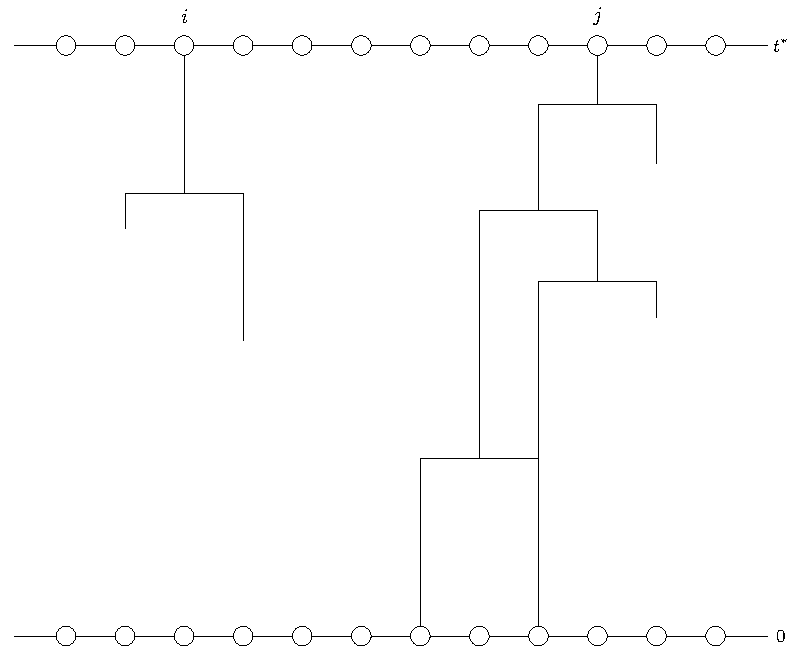
\includegraphics[width = 0.8\textwidth]{Figures/IsingCouplingTime/typical_percolation.pdf}
		\caption[Typical appearance of the update histories for two vertices on the cycle]{A section of the space-time slab $V \times [0, t_*]$ along with a typical appearance of the update histories for two vertices on the cycle. Time runs vertically from bottom to top, and the vertices are represented by circles, laid out horizontally. If there is a path in the update history of $v$ between points $(u, t)$ and $(v, t_*)$, then the spin of $v$ at time $t_*$ depends on the spin of $u$ at time $t$. In this example, since there is no path from vertex $(i, t_*)$ to time $0$, the final spin at $i$ does not depend on the initial configuration whereas the final spin at $j$ does.}
		\label{fig:typical percolation}
	\end{figure}

	\subsubsection{The update sequence}
	Recalling our random mapping representation from Section \ref{sec:the coupling time}, we can encode an update of our coupled process with the tuple $(\mathcal{V}, U, S)$, where $S$ is the time of the update, $\mathcal{V}$ is the vertex that is updated, and $U$ is the value of the uniform random variable that tells us whether $\mathcal{V}$ is a plus or minus according to \eqref{eq:plusorminusrules}. The \emph{update sequence} along an interval $(t_0, t_1]$ is the set of these tuples with $t_0 < S \leq t_1$, ordered by $S$ decreasing from $t_1$. 

	Let $(Y_t)_{t \geq 0}$ be a copy of the continuous-time heat-bath Glauber dynamics starting in some state $Y_0 \in \Omega$. So $Y_t = \mathscr{T}_t$ if $Y_0 = (1, 1, \dots, 1)$ and $Y_t = \mathscr{B}_t$ if $Y_0 = (-1, -1, \dots, -1)$. Given the state of $Y$ at time $t_0$, $Y_{t_0}$, the update sequence along $(t_0, t_1]$ contains all the information we need to construct $Y_{t_1}$. In particular, given the update sequence along the interval $(0, t_1]$, $Y_{t_1}$ is a deterministic function of $Y_0$.

	\subsubsection{The update support function}
	\label{sec: definition update support function}
	Given the update sequence along the interval $(t_1, t_2]$, the \emph{update support function}, $\mathscr{F}(A, t_1, t_2)$, is the minimal set of vertices whose spins at time $t_1$ determine the spins of the vertices in $A$ at time $t_2$. That is, $i \in \mathscr{F}(A, t_1, t_2)$ if and only if there exist states $Y_{t_1}, Y_{t_1}' \in \{-1, +1\}^{V}$ that differ only at $i$ and such that when we construct $Y_{t_2}$ and $Y_{t_2}'$ using the update sequence, $Y_{t_2} \neq Y_{t_2}'$.

	In particular, if $\mathscr{F}(i, 0, t) = \emptyset$ then the spin at vertex $i$ at time $t$ does not depend on the initial state and so for our coupled chains, $\mathscr{B}_t[i] = \mathscr{T}_t[i]$.
	% It follows that
	% \begin{equation}
	% 	\prob \left[ Y_t[v] \neq Y_t'[v] \right] \leq \prob \left[ \mathscr{F}(v, 0, t) \neq \emptyset \right].
	% 	\label{eq:boundXneqY}
	% \end{equation}
	As a consequence of the monotonicity of our coupling, we can make the stronger statement that $\mathscr{T}_t[i] = \mathscr{B}_t[i]$ if and only if $\mathscr{F}(i, 0, t) = \emptyset$ which of course means that
	\begin{equation}
	\label{eq:prob equality of coupling and empty support}
		\prob[\mathscr{T}_t[i] \neq \mathscr{B}_t[i]] = \prob[\mathscr{F}(i, 0, t) \neq \emptyset].
	\end{equation}

	For ease of notation, we will often use the shorthand
	\begin{equation}
		\mathcal{H}_i(t) := \mathscr{F}(i, t, t_*)
	\end{equation}
	where $t_*$ is some target time that should be clear from context. We call this the \emph{update support} of vertex $i$ at time $t$. Tracing $\mathcal{H}_i(t)$ backwards in time from $t_*$ produces a subgraph of $V \times [0, t_*]$ which we write as $\mathcal{H}_i$ and which we call the \emph{update history} of vertex $i$. To be slightly more precise, to produce $\mathcal{H}_i$ we connect $(j,t)$ to $(j,t')$ if $j \in \mathcal{H}_i(t)$ and there are no updates of $j$ along $(t', t]$ and we connect $(j,t)$ to $(j',t)$ if there was an update at $(j, t)$, $j \in \mathcal{H}_i(t)$, $j' \notin \mathcal{H}_i(t)$, and $j' \in \mathcal{H}_i(t-\epsilon)$ for all sufficiently small $\epsilon > 0$.

	Similarly, we also use 
	\begin{equation}
		\hist_A(t) := \mathscr{F}(A, t, t_*)
	\end{equation}
	for the update history of a vertex set $A$ at time $t$ and $\hist_A$ for the update history of vertex set $A$. Note that
	\begin{equation}
		\hist_A(t) = \bigcup_{i \in A} \hist_i(t)
	\end{equation}
	and 
	\begin{equation}
		\hist_A = \bigcup_{i \in A} \hist_i.
	\end{equation}

	% ALSO DEFINE UPDATE SUPPORT
	
	\subsubsection{The update function}
	\label{sec: definition update function}
	It is usually non-trivial to construct the update support function from the update sequence. So in order to give some intuition to the definitions above, we describe another function which contains the update support and which is simple to construct. We define the \emph{update function}, $\mathscr{F}_\mathrm{UPD}(A, t_1, t_2)$, to be the set of all vertices that $A$ can `reach' through the update function. That is, $i \in \mathscr{F}_\mathrm{UPD}(A, t_1, t_2)$ if and only if there exists a subsequence of the updates, $(\mathcal{V}_k, U_k, S_k)$, such that $t_1 < S_1 < S_2, \dots, \leq S_m$ and $i, \mathcal{V}_1, \mathcal{V}_2, \dots, \mathcal{V}_m$ is a path connecting $i$ to some vertex $\mathcal{V}_m \in A$. 

	Just as we traced the update support backwards through time to create the update history, we can also trace $\mathscr{F}_\mathrm{UPD}(i, t, t_*)$ backwards through time to create the analogous \emph{update trace}, $\mathcal{G}_i$. It is clear that $\mathscr{F}(A, t_1, t_2) \subseteq \mathscr{F}_\mathrm{UPD}(A, t_1, t_2)$ since a vertex $i$ can only affect the spins of $A$ if there is a path of updates connecting it to $A$. Likewise we also have that $\mathcal{G}_i \subseteq \hist_i$.
	
	Consider how we can construct the update trace of a vertex $i$ from some target time $t_*$. We have at our disposal the update sequence along $(0, t_*]$ which is placed in order of decreasing time. If vertex $i$ does not appear in the update sequence then we create a temporal edge between $(i, t_*)$ and $(i, 0)$ and our update history is complete. Otherwise, we create a temporal edge between $(i, t_*)$ and $(i, t_i)$ where $t_i$ is the last time vertex $i$ was updated. At this point we add spatial edges from $(i, t_i)$ to $(j, t_i)$ for each $j\sim i$. Then, we iterate this process for $i$ and each of its neighbours starting at time $t_i$ until every edge has reached time $0$. In Figure \ref{fig:example trace construction} we have followed this procedure to show an example update trace for a single vertex on the cycle. 

	\begin{figure}
		\centering
		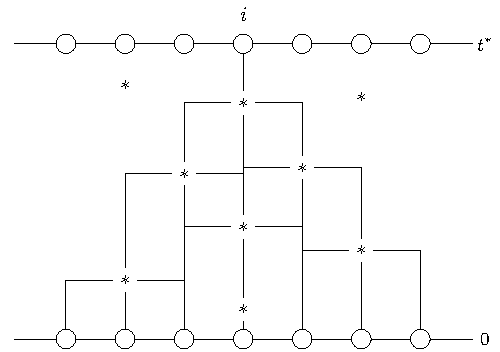
\includegraphics[width = 0.8\textwidth]{Figures/IsingCouplingTime/example_update_trace_construction.pdf}
		\caption[The update trace of i]{The update trace of $i$. Each update $(\mathcal{V}, U, t)$ in the update sequence is represented by a $*$ at $(\mathcal{V}, t)$.}
		\label{fig:example trace construction}
	\end{figure}

	We turn now to discussing how the update history differs from the update trace. We first note that an update to vertex $i$ removes it from the update support as we move backwards in time. This is because the updated spin at $i$ is a function only of its neighbours \eqref{eq:plusorminusrules}. The second difference which we will now spend some time discussing is that it is possible for updates to occur that do not depend on neighbouring spins. These updates therefore cause temporal edges leading up to them to terminate without branching out to the neighbouring vertices. These type of updates are called \emph{oblivious updates}. (These are not the only differences between the update history and the update trace; there are other ways in which vertices can be removed from the update support. See Figure \ref{fig:nonoblivious shrink} for an example).

	% \begin{figure}
	% 	\centering
	% 	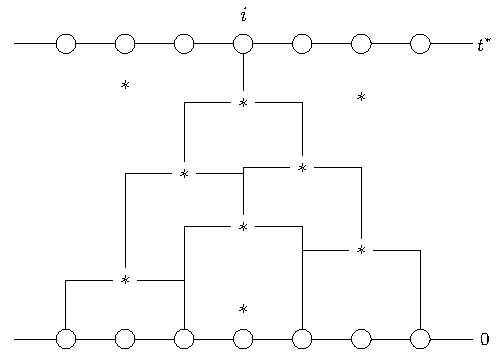
\includegraphics[width = 0.8\textwidth]{Figures/IsingCouplingTime/example_percolation_construction.pdf}
	% 	\caption[A naive construction of the update history of i]{A naive construction of the update history of $i$. Each update $(\mathcal{V}, U, t)$ in the update sequence is represented by a $*$ at $(\mathcal{V}, t)$.}
	% 	\label{fig:example percolation construction}
	% \end{figure}

	

	\subsubsection{Oblivious updates}
	\label{sec:oblivious updates}

	Roughly speaking, an update to a vertex is oblivious if we do not need to know the configuration of its neighbours to determine the spin of that vertex. More precisely, an update, $(\mathcal{V}, U, t)$, is oblivious if and only if
	%for any $\sigma_1, \sigma_2 \in \Omega$, $\sigma_1' = f(\sigma_1, \mathcal{V}, U)$ and $\sigma_2' = f(\sigma_2, \mathcal{V}, U)$ are such that
	% \begin{equation}
	% 	\sigma_1'[\mathcal{V}] = \sigma_2'[\mathcal{V}].
	% \end{equation}
	\begin{equation}
		f(\sigma, \mathcal{V}, U)[\mathcal{V}] = f(\sigma', \mathcal{V}, U)[\mathcal{V}]
	\end{equation}
	for all $\sigma, \sigma' \in \Omega$, where $f$ is as defined in \eqref{eq:plusorminusrules}.

	Consider how these updates occur under our random mapping representation. Let $\Delta_i$ denote the degree of a vertex $i$. Recalling \eqref{eq:define p_i},
	\begin{equation}
		\frac{\euler^{-\beta \Delta_i}}{\euler^{\beta \Delta_i} + \euler^{-\beta \Delta_i}} \leq p_i(\sigma) \leq \frac{\euler^{\beta \Delta_i}}{\euler^{\beta \Delta_i} + \euler^{-\beta \Delta_i}},
	\end{equation}
	with equality holding for the lower and upper limits when the neighbours have spins all minus and all plus respectively. So for a particular update $(\mathcal{V}, U, t)$, if $U \leq \frac{\euler^{-\beta \Delta_\mathcal{V}}}{\euler^{\beta \Delta_\mathcal{V}} + \euler^{-\beta \Delta_\mathcal{V}}}$ then $\mathcal{V}$ is updated to a plus regardless of the configuration of its neighbours. Hence $(\mathcal{V}, U, t)$ is an oblivious update. Similarly, if $U > \frac{\euler^{\beta \Delta_\mathcal{V}}}{\euler^{\beta \Delta_\mathcal{V}} + \euler^{-\beta \Delta_\mathcal{V}}}$ then $\mathcal{V}$ is updated to a minus regardless of the configuration of its neighbours and hence $(\mathcal{V}, U, t)$ is an oblivious update. It is easy to see that these are the only types of oblivious updates.
	
	Given an update at vertex $i$, the probability that this update is oblivious is
	\begin{align}
		\theta_i &= 1 - \left(\frac{\euler^{\beta \Delta_i}}{\euler^{\beta \Delta_i} + \euler^{-\beta \Delta_i}} - \frac{\euler^{-\beta \Delta_i}}{\euler^{\beta \Delta_i} + \euler^{-\beta \Delta_i}}\right)\\
			&= 1 - \tanh(\beta \Delta_i).
	\end{align}
	If $G$ is a $\Delta$-regular graph (as will be the case in the following chapters) then we can drop the subscript and write $\theta = 1 - \tanh(\beta \Delta)$ for the probability of an oblivious update at each vertex.

	As noted earlier, oblivious updates cause temporal edges leading to them in the update history to terminate. If $j \in \mathcal{H}_i(t)$, then an oblivious update $(j, u, t)$ removes $j$ from $\mathcal{H}_i(t)$ without adding any of its neighbours. In Figure \ref{fig:example percolation construction oblivious} we construct the update history from a single vertex $i$ using the same update sequence as in Figure \ref{fig:example trace construction} but instead of representing each update with just a $*$, we give a little more information in the following way. Note that on the cycle, the function defined in \eqref{eq:plusorminusrules} can be rewritten as
	\begin{equation}
		\sigma'[i] = 
		\begin{cases}
			1 & U \leq \theta/2,\\
			\sigma[i-1] \vee \sigma[i+1] & \theta/2 < U \leq 1/2,\\
			\sigma[i-1] \wedge \sigma[i+1] & 1/2 < U \leq 1 - \theta/2,\\
			-1	& U > \theta/2.
		\end{cases}
	\end{equation}
	We can therefore represent each update $(\mathcal{V}, U, t)$ in the update sequence by placing at $(\mathcal{V}, t)$ one of the symbols $+$, $\vee$, $\wedge$, or $-$ chosen according to $U$. We then trace back from time $t_*$, branching to either side when we encounter a $\vee$ or $\wedge$, and terminating whenever we encounter a $+$ or $-$.

	\begin{figure}
		\centering
		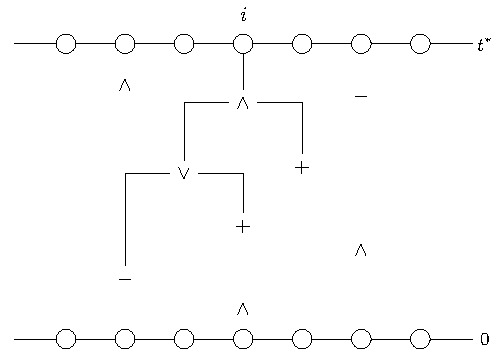
\includegraphics[width = 0.8\textwidth]{Figures/IsingCouplingTime/example_percolation_construction_oblivious.pdf}
		\caption[The update sequence for a section of the cycle and the corresponding update history from vertex i]{The update sequence for a section of the cycle and the corresponding update history from vertex $i$. For this particular update sequence, $i$ takes a final spin of $+1$ regardless of the initial configuration.}
		\label{fig:example percolation construction oblivious}
	\end{figure}

	
	It is worth remarking that oblivious updates are not necessarily the only updates that can shrink the size of the update history of $i$. In Figure \ref{fig:nonoblivious shrink} we use an example from \cite{Lubetzky2016-wd} that shows the update support collapsing down to a single vertex from a non-oblivious update. However, for our analysis, oblivious updates will be the only such updates we will be concerned with. Indeed, in Chapter \ref{Ch:1D} we will use a different coupling so that these are the only updates that shrink the size of the update history, and in Chapter \ref{Ch:GeneralResults} we will use an alternative construction that bounds the true update history, in which all updates are either oblivious or branch out to all $\Delta$ neighbours.

	\begin{figure}
		\centering
		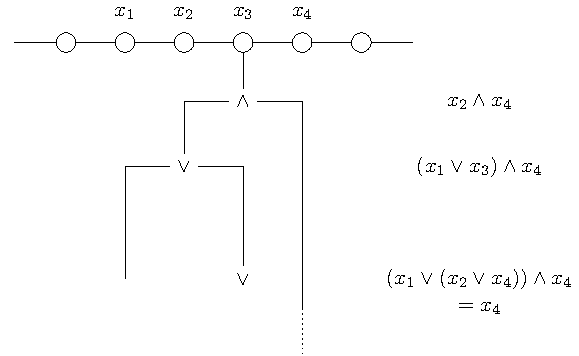
\includegraphics[width = 0.8\textwidth]{Figures/IsingCouplingTime/nonoblivious_shrink.pdf}
		\caption[A non-oblivious update that shrinks the size of the update history]{[Example taken from \cite{Lubetzky2016-wd}]. A non-oblivious update that shrinks the size of the update history. On the right is written the final spin of $x_3$ as a function of the configuration at that time. The update $x_3 \mapsto x_2 \vee x_4$ causes the entire function to collapse to $x_4$, and so removes $x_1$ and $x_3$ from the update history.}
		\label{fig:nonoblivious shrink}
	\end{figure}
	

\section{Compound Poisson approximation}
\label{sec:compound poisson overview}
	In addition to the framework of information percolation, we will also make use of compound Poisson approximation, as described in \cite{Barbour2001-nh}. This paper reviews a number of methods by which approximations may be made. The specific method that we will employ is based on Stein's method for the compound Poisson distribution, introduced in \cite{Barbour1992-mc}.

	A compound Poisson distribution, $\mathrm{CP}(\lambda, \vect{\mu})$, is the distribution of the sum of a rate $\lambda$ Poisson number of independent random variables, each with distribution $\vect{\mu}$. That is, a compound Poisson random variable can be defined by
	\begin{equation}
		\mathrm{CP}(\lambda, \vect{\mu}) = \mathscr{L}\left(\sum_{j=1}^M Y_j\right)
	\end{equation}
	for any $\lambda > 0$, and any probability distribution $\mu$ on $\mathbb{N}$, where the $Y_j$ are independent and identically distributed with distribution $\vect{\mu}$ and are also independent of $M \sim \mathrm{Po}(\lambda)$.

	The goal of compound Poisson approximation is to bound the distance between the distribution of a random variable $W$, and some canonically chosen compound Poisson distribution. A common scenario, and the one which we address here, is that
	\begin{equation}
		W = \sum_{i \in V} X_i
	\end{equation}
	for some countable index set $V$, where each $X_i$ is a nonnegative integer valued random variable. The following approach to compound Poisson approximation is taken from \cite[Section 2.2]{Barbour2001-nh}.

	For each $i \in V$, partition $V$ into subsets $\{i\}$, $B_i$, $C_i$, and $D_i$ and set 
	\begin{align}
		U_i &= \sum_{j \in B_i} X_j, &
		Z_i &= \sum_{j \in C_i} X_j, &
		W_i &= \sum_{j \in D_i} X_j.
	\end{align}
	so that for each $i \in V$ we have the decomposition 
	\begin{equation}
		W = X_i + U_i + Z_i + W_i.
	\end{equation}
	For our approximation to be good, we want $B_i$ to contain those $X_j$ which strongly influence $X_i$, $D_i$ to contain those $X_j$ which have a negligible effect on $X_i$ and $C_i$ to contain the remainder.

	Using $\indicator[\cdot]$ to denote the indicator function, we now define the canonical parameters $\lambda$ and $\vect{\mu}$ by
	\begin{align}
		\lambda &= \sum_{i \in V} \expect\left[\frac{X_i}{X_i + U_i} \, \indicator[ X_i + U_i \geq 1] \right],\\
		\mu_l &= \frac{1}{l \lambda} \sum_{i \in V} \expect\left[ X_i \, \indicator[X_i + U_i = l] \right], && l\geq 1.
		\label{eq:mu definition}
	\end{align}
	These will be the parameters of the approximating compound Poisson distribution to $W$. We also define
	\begin{align}
		\delta_1 &= \sum_{i \in V}  \sum_{k \geq 0} \prob[X_i = 1, U_i = k] \expect \left|\frac{\prob[X_i = 1, U_i = k|W_i]}{\prob[X_i = 1, U_i = k]} - 1 \right|, \label{eq:delta_1 definition}\\ 
		% \delta_2 &= \\
		% \delta_3 &= \\
		\delta_4 &= \sum_{i \in V} \left( \expect[X_i Z_i] + \expect[X_i] \expect[X_i + U_i + Z_i] \right), \label{eq:delta_4 definition}
	\end{align}
	% which we will require to vanish as $n \rightarrow \infty$.
	which we desire to be small for the compound Poisson approximation to be good.

	We can bound the total variation distance between $W$ and the canonically chosen compound Poisson using the following theorem, reworked from \cite[CPA 1A]{Barbour2001-nh} with bounds for the constants provided there substituted from \cite[Equation 2.17]{Barbour2001-nh}.

	\begin{theorem}[\cite{Barbour2001-nh}]
	\label{thm: compound poisson approximation}
		Let $W$, $\lambda$, $\vect{\mu}$, $\delta_1$ and $\delta_4$ be as defined above. Then
		\begin{equation}
			d_{\mathrm{TV}}(\mathscr{L}(W), \mathrm{CP}(\lambda, \vect{\mu})) \leq (\delta_1 + \delta_4)\euler^\lambda.
		\end{equation}
	\end{theorem}

	Since the canonical parameter $\vect{\mu}$ is constructed to only place mass on the positive integers, we have that
	\begin{align}
		\prob\left(\mathrm{CP}(\lambda, \vect{\mu}) = 0\right) &= \prob\left(\mathrm{P}(\lambda) = 0 \right) \\
		&= \euler^{-\lambda}.
	\end{align}
	This gives us the following corollary of Theorem \ref{thm: compound poisson approximation}.

	\begin{corollary}
	\label{cor: bound prob W = 0}
		Let $W$, $\lambda$, $\delta_1$ and $\delta_4$ be as defined above. Then
		\begin{equation}
			\left|\prob\left(W = 0\right) - \euler^{-\lambda}\right| \leq (\delta_1 + \delta_4)\euler^\lambda.
		\end{equation}
	\end{corollary}

	\subsection{Application to our problem}
	\label{sec:application of compound poisson}
	We will now give an overview of how we will apply compound Poisson approximation to the problem of finding the limiting distribution of the coupling time of the Ising heat-bath process. The exact implementation will depend on the class of graphs on which the heat-bath process is running, and so we leave some of the specifics for the following chapters.

	For a given graph, $G_L = (V, E)$, in a given sequence of graphs, $(G_L)_{L \geq 1}$, we fix $z \in \mathbb{R}$ and a time of interest 
	\begin{equation}
		t_* = a_L z + d_L.
	\end{equation}
	The specific choices for $a_L$ and $d_L$ depend on the sequence $(G_L)_{L \geq 1}$. We choose these such that for large enough $L$, $t_* > 0$, and then only consider these $L$. For each $i \in V$, define the indicator
	\begin{equation}
		X_i = \indicator\left[\mathscr{B}_{t_*}[i] \neq \mathscr{T}_{t_*}[i]\right]
	\end{equation}
	and set 
	\begin{equation}
		W = \sum_{i \in V} X_i.
	\end{equation}
	For each $i \in V$, we partition $V$ into the sets $\{i\}, B_i, C_i$, and $D_i$ defined by
	\begin{align}
		B_i &= \{j\neq i : d(i,j) \leq b_L \},\\
		C_i &= \{j\notin B_i\cup \{i\}: d(i,j) \leq c_L \},\\
		D_i &= V \setminus (B_i \cup C_i \cup \{i\}),
	\end{align}
	where we use $d(i, j)$ to denote the graph distance between vertices $i$ and $j$. The specific choices for $b_L$ and $c_L$ again depend on the graph $G_L$.

	We can now define $U_i, Z_i$, and $W_i$ as above, along with $\lambda, \vect{\mu}, \delta_1$, and $\delta_4$. We can then directly apply Theorem \ref{thm: compound poisson approximation} to get that
	\begin{equation}
		d_{\mathrm{TV}}(\mathscr{L}(W), \mathrm{CP}(\lambda, \vect{\mu})) \leq (\delta_1 + \delta_4)\euler^\lambda.
	\end{equation}


	To relate $W$ to the coupling time, observe that $W$ is zero precisely when $T \leq t_*$ and so the events $\{W = 0\}$ and $\{T \leq t_*\}$ coincide. So using Corollary \ref{cor: bound prob W = 0},
	\begin{equation}
		\label{eq:bound distribution T}
		\left|\prob\left(T \leq t_*\right)  - \euler^{-\lambda}\right| \leq (\delta_1 + \delta_4) \euler^\lambda.
	\end{equation}
	The bulk of the work is therefore in calculating $\lambda$, and in showing that $\delta_1$ and $\delta_4$ go to zero as $L \rightarrow \infty$. (Note that $W, T, t_*, \lambda, \vect{\mu}, \delta_1$, and $\delta_4$ all depend on $L$ but we have omitted this in the notation for convenience).

%---results chapter---
% 1D results
%!TEX root = ..\..\main.tex
\chapter{The Coupling Time on the Cycle}
\label{Ch:1D}

\lhead{Chapter \ref{Ch:1D}. \emph{The Coupling Time on the Cycle}}

	In this chapter we consider the Ising heat-bath Glauber dynamics (as described in Section \ref{sec:heat-bath glauber dynamics definition}) on the cycle $G_n = (\mathbb{Z}/n\mathbb{Z})$. The object of interest is the coupling time, $T_n$, which was defined in Section \ref{sec:the coupling time} but whose definition will be modified slightly in Section \ref{sec:information percolation on the cycle} to allow for simpler analysis. The main result establishes that $T_n$ converges in distribution to a Gumbel distribution at all temperatures. This confirms, for $d = 1$, a conjecture by \citeauthor{Collevecchio2017-nq} that the coupling time of the Ising heat-bath process on the lattice $G_L = (\mathbb{Z}/L\mathbb{Z})^d$ converges to a Gumbel distribution as $L \rightarrow \infty$ for all $\beta < \beta_C$ \cite[Conjecture 7.1]{Collevecchio2017-nq} (We treat higher dimensions, and more generally any vertex transitive graphs, in Chapter \ref{Ch:GeneralResults}). Of course, in one dimension, all temperatures are part of the high temperature regime [CITE], and likewise our result holds for any inverse-temperature $\beta$.

	\begin{theorem}
	\label{thm:Coupling Distribution on Cycle}
		Let $T_n$ be the coupling time for the continuous-time Ising heat-bath Glauber dynamics for the zero-field ferromagnetic Ising model on the cycle $(\mathbb{Z} / n\mathbb{Z})$. Then for any inverse-temperature $\beta$,
		\begin{equation}
			\lim_{n \rightarrow \infty} \prob\left[T_n < \frac{z + \ln n}{\theta}\right] = \euler^{-C_\theta \euler^{-z}}
		\end{equation}
		where $\theta = 1 - \tanh(2\beta)$ and $C_\theta$ is a positive constant bounded by
		\begin{equation}
			\frac{1}{2\sqrt{\frac{4}{\theta} - 1} - 1} \leq \lambda \leq 1.
		\end{equation}
	\end{theorem}

	The proof of Theorem \ref{thm:Coupling Distribution on Cycle} will be given in Section \ref{sec:proof thm coupling cycle} after the essential preliminaries are presented.

	[INTUITIVE HANDWAVING 'ROADMAP' OF PROOF]

	[WHAT IT MEANS]

	[WHATS THE POINT?]

	\section{A new coupling on the cycle}
	\label{sec:information percolation on the cycle}
	% On the cycle, the heat-bath dynamics allow for a new set of updates rules, to replace those from \eqref{eq:plusorminusrules}. The changed update rules provide another construction for the coupling of $\mathscr{T}_t$ and $\mathscr{B}_t$ but preserve the distribution of the coupling time, $T_n$. We use these new update rules because they result in much simpler update histories.

	On the cycle, we will use a different coupling of $\mathscr{T}_t$ and $\mathscr{B}_t$ via a new set of update rules that will replace those from \eqref{eq:plusorminusrules}. The new update rules simplify our update histories greatly by ensuring that each of the update histories never contain more than one vertex at any one time. However, we must be cautious. The coupling time is not just a property of the heat-bath dynamics, but also of the specific coupling we chose. Hence, we will have to verify that switching to our new rules does not change the distribution of $T_n$. 

	The new update rules are defined by using almost the same construction as in Section \ref{sec:the coupling time}. The one difference is that we replace \eqref{eq:plusorminusrules} as follows. When vertex $i$ updates, instead of comparing $U$ to the probability $p_i(\sigma)$ to determine the new spin, we instead chose a new spin $\sigma_i'$ via
	% state that when vertex $i$ updates, a spin $\sigma_i'$ is chosen via
	\begin{equation}
	\label{eq:new update rules}
		\sigma_i' = \begin{cases}
			+1 & U < \theta/2,\\
			\sigma_{i-1} & \theta/2 \leq U < 1/2,\\
			\sigma_{i+1} & 1/2 \leq U < 1 - \theta/2,\\
			-1 & U \geq 1 - \theta/2.
		\end{cases}
	\end{equation}
	where $U \in [0,1]$ is an independent uniform random variable as before. It is easy to see that these update rules give rise to the same transition rates as those in \eqref{eq:plusorminusrules}. To show that the coupling time is unchanged, it is sufficient to verify that the joint jump probabilities of $(\mathscr{T}_t[i], \mathscr{B}_t[i])$ are unchanged for each possible configuration of spins of vertices $i-1$ and $i+1$. There are only nine possible configurations for the two neighbours of $i$ in the top and bottom chain since $\mathscr{B}_t[i] \leq \mathscr{T}_t[i], \forall t$. Likewise, there are only three possible configurations for the updated spins $(\mathscr{T}_t[i]', \mathscr{B}_t[i]')$. Hence, given vertex $i$ updates at time $t$, we can easily calculate all the required jump probabilities as shown in Table \ref{tab: joint jump probs}. These are unchanged whether using \eqref{eq:plusorminusrules} or \eqref{eq:new update rules} and so the new rules do not change the coupled dynamics.

	\begin{table}
	\begin{tabular}{c || c c c}
	\diagbox[]{		
		\begin{tabular}{@{}c@{}}
		$\mathscr{T}_t = \cdot$ \\ 
		$\mathscr{B}_t = \cdot$ 
		\end{tabular}
	}{
		$\prob[(\mathscr{T}_t[i]', \mathscr{B}_t[i]') = \cdot \,]$
	}
	&(1,1)&(1,-1)&(-1,-1)\\
	\hline
	\hline
		\begin{tabular}{@{}c@{}}
		$(\dots, 1, \sigma_i, 1,\dots)$ \\ 
		$(\dots, 1, \sigma_i, 1,\dots)$ 
		\end{tabular}
	&$1 - \theta$& 0 & $\frac{\theta}{2}$\\
	\hline
		\begin{tabular}{@{}c@{}}
		$(\dots, 1, \sigma_i, 1,\dots)$ \\ 
		$(\dots, 1, \sigma_i, -1,\dots)$ 
		\end{tabular}
	&$\frac{1}{2}$& $\frac{1-\theta}{2}$ & $\frac{\theta}{2}$\\
	\hline
		\begin{tabular}{@{}c@{}}
		$(\dots, 1, \sigma_i, 1,\dots)$ \\ 
		$(\dots, -1, \sigma_i, 1,\dots)$ 
		\end{tabular}
	&$\frac{1}{2}$& $\frac{1-\theta}{2}$ & $\frac{\theta}{2}$\\
	\hline
		\begin{tabular}{@{}c@{}}
		$(\dots, 1, \sigma_i, 1,\dots)$ \\ 
		$(\dots, -1, \sigma_i, -1,\dots)$ 
		\end{tabular}
	& $\frac{\theta}{2}$ & $1 - \theta$ & $\frac{\theta}{2}$ \\
	\hline
		\begin{tabular}{@{}c@{}}
		$(\dots, 1, \sigma_i, -1,\dots)$ \\ 
		$(\dots, 1, \sigma_i, -1,\dots)$ 
		\end{tabular}
	& $\frac{1}{2}$ & 0 & $\frac{1}{2}$ \\
	\hline
		\begin{tabular}{@{}c@{}}
		$(\dots, 1, \sigma_i, -1,\dots)$ \\ 
		$(\dots, -1, \sigma_i, -1,\dots)$ 
		\end{tabular}
	& $\frac{\theta}{2}$ & $\frac{1-\theta}{2}$ & $\frac{1}{2}$ \\
	\hline
		\begin{tabular}{@{}c@{}}
		$(\dots, -1, \sigma_i, 1,\dots)$ \\ 
		$(\dots, -1, \sigma_i, 1,\dots)$ 
		\end{tabular}
	& $\frac{1}{2}$ & 0 & $\frac{1}{2}$ \\
	\hline
		\begin{tabular}{@{}c@{}}
		$(\dots, -1, \sigma_i, 1,\dots)$ \\ 
		$(\dots, -1, \sigma_i, -1,\dots)$ 
		\end{tabular}
	& $\frac{\theta}{2}$ & $\frac{1-\theta}{2}$ & $\frac{1}{2}$ \\
	\hline
		\begin{tabular}{@{}c@{}}
		$(\dots, -1, \sigma_i, -1,\dots)$ \\ 
		$(\dots, -1, \sigma_i, -1,\dots)$ 
		\end{tabular}
	& $\frac{\theta}{2}$ & 0 & $1 - \theta$
	\end{tabular}
	\caption{Probabilities of updating from $(\mathscr{T}_t, \mathscr{B}_t)$ to $(\mathscr{T}_t', \mathscr{B}_t')$ given vertex $i$ updates at time $t$.}
	\label{tab: joint jump probs}
	\end{table}
	% It is easy to verify that for each possible configuration, the joint distribution for $\sigma_i'$ in the top and bottom chains is the same whether we use these rules or the ones given in \eqref{eq:plusorminusrules}. Hence the coupling time is unchanged in distribution in this new random mapping representation.

	\subsection{Update histories on the cycle}
	Under the update rules in \eqref{eq:new update rules}, each time a vertex is updated, it is either an oblivious update with probability $\theta$, or it takes the spin of a uniformly chosen neighbour. Unlike the histories considered earlier (for example Figure \ref{fig:example percolation construction oblivious}), this time a non-oblivious update does not cause the history to branch out to both its neighbours. Rather, given a non-oblivious update to some vertex $v$, we only need to know the spins of one of its neighbours to update it (the left spin if $U  < 1/2$ and the right if $U \geq 1/2$). So the history simply moves either right or left without branching. As before, encountering an oblivious update causes $\mathcal{H}_i$ to terminate. An example history using these new rules is shown in Figure \ref{fig:example percolation construction rightleft}. In a similar vein to Figures \ref{fig:example percolation construction oblivious} and \ref{fig:nonoblivious shrink} we represent each update $(\mathcal{V}, U, t)$ in the update sequence by placing at $(\mathcal{V}, t)$ one of the symbols $+$, $r$, $l$, or $-$ choosen according to $U$. We then trace back from time $t^*$, moving left or right when we encounter a $l$ or $r$ respectively, and terminating whenever we encounter a $+$ or $-$.

	\begin{figure}
		\centering
		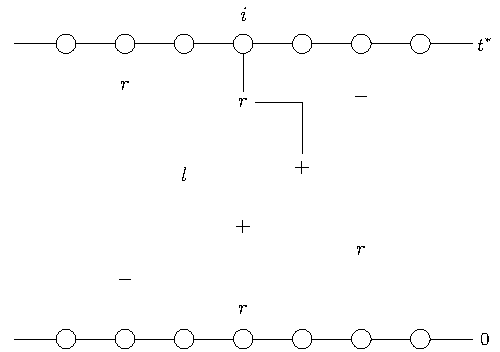
\includegraphics[width = 0.8\textwidth]{Figures/IsingCouplingTime/example_percolation_construction_rightleft.pdf}
		\caption[The update sequence for a section of the cycle and the corresponding update history from vertex i using the new update rules.]{The update sequence for a section of the cycle and the corresponding update history from vertex $i$ using the new update rules. Vertex $i$ takes the same spin as the spin it terminates at, in this case $+1$.}
		\label{fig:example percolation construction rightleft}
	\end{figure}

	We now see that as $t$ decreases from $t^*$, $\mathcal{H}_i(t)$ is a continuous-time random walk that dies at rate $\theta$, moves left at rate $(1 - \theta)/2$, and moves right at rate $(1 - \theta)/2$. The probability that $\mathcal{H}_i(0) \neq \emptyset$ is simply the probability that the continuous-time random walk survives until time $t = 0$. This immediately gives us the following probability which we will use repeatedly in what follows. Recalling \eqref{eq:prob equality of coupling and empty support},
	\begin{equation}
		\prob \left[ \mathscr{B}_{t^*}[i] \neq \mathscr{T}_{t^*}[i] \right] = 
		\prob \left[ \mathcal{H}_i(0) \neq \emptyset \right] = 
		\euler^{-\theta t^*}.
		\label{eq:1D bernoulli prob}
	\end{equation}
	since our histories die at rate $\theta$.

	\section{Problem Setup}
	In order to prove Theorem \ref{thm:Coupling Distribution on Cycle}, we will actually prove a stronger statement using Theorem \ref{thm: compound poisson approximation}. The general idea is that at some fixed time $t^*$ we will count the number of vertices at which the bottom and top chains differ. This number is a random variable, which we will call $W$, and we can bound the total variation distance of its distribution with that of an appropriate compound poisson distribution. As a special case, we can use this bound as a bound on the probability that $W$ is zero. Of course, if $W$ is zero then the top and bottom chains must have coupled and so we can use this to establish Theorem \ref{thm:Coupling Distribution on Cycle}.

	Bounding the total variation distance between $W$ and the compound Poisson will be done using compound Poisson approximation as described in \cite{Barbour2001-nh}. This paper reviews a number of different methods by which approximations may be made. The specific method that we will employ is based on Stein's method for the compound Poisson distribution, introduced in \cite{Barbour1992-mc}.

	We now make precise the ideas stated above.	Fix $z$ and a time of interest, $t_* = (z + \ln n)/\theta$. For each vertex $i \in G$, define indicators
	\begin{equation}
		X_i = 
		\begin{cases}
			1 & \mathscr{B}_{t^*}[i] \neq \mathscr{T}_{t^*}[i],\\
			0 & \mathscr{B}_{t^*}[i] = \mathscr{T}_{t^*}[i]
		\end{cases}
	\end{equation}
	and set $W = \sum_{i \in V} X_i$.
	Note that from \eqref{eq:1D bernoulli prob} we get
	\begin{equation}
		\label{eq:1D prob X_i}
		\prob[X_i = 1] = \euler^{-\theta t_*} = \frac{e^{-z}}{n}.
	\end{equation}
	% We create vertex sets
	% \begin{align}
	% 	B_i &= \{j\neq i : |j - i| \leq b_n \},\\
	% 	C_i &= \{j\notin B_i\cup \{i\}: |j - i| \leq c_n \},\\
	% 	D_i &= V \setminus (B_i \cup C_i \cup \{i\}).
	% \end{align}
	% where $b_n = \ln(n)$ and $c_n = \ln(n)^2$. 
	For each $i \in V$, decompose $W$ into $W = X_i + U_i + Z_i + W_i$ where
	\begin{align}
		U_i &= \sum_{j \in B_i} X_j, &
		Z_i &= \sum_{j \in C_i} X_j, &
		W_i &= \sum_{j \in D_i} X_j.
	\end{align}
	and $B_i, C_i$, and $D_i$ are the vertex sets
	\begin{align}
		B_i &= \{j\neq i : |j - i| \leq b_n \},\\
		C_i &= \{j\notin B_i\cup \{i\}: |j - i| \leq c_n \},\\
		D_i &= V \setminus (B_i \cup C_i \cup \{i\}).
	\end{align}
	We have some freedom in choosing $b_n$ and $c_n$; they are chosen to control the assymptotics of various quantities to be defined later. For this chapter, we will choose $b_n = \ln(n)$ and $c_n = \ln(n)^2$.

	We now define the quantities
	\begin{align}
		\lambda &= \sum_{i \in V} \expect\left[\frac{X_i}{X_i + U_i} \indicator[ X_i + U_i \geq 1] \right],\\
		\mu_l &= \frac{1}{l \lambda} \sum_{i \in V} \expect\left[ X_i \indicator[X_i + U_i = l] \right], && l\geq 1,
		\label{eq:mu definition}
	\end{align}
	which will be the parameters of the approximating compound Poisson distribution to $W$. We also define
	\begin{align}
		\delta_1 &= \sum_{i \in V}  \sum_{k \geq 0} \prob[X_i = 1, U_i = k] \expect \left|\frac{\prob[X_i = 1, U_i = k|W_i]}{\prob[X_i = 1, U_i = k]} - 1 \right|, \label{eq:1D delta_1 definition}\\ 
		% \delta_2 &= \\
		% \delta_3 &= \\
		\delta_4 &= \sum_{i \in V} \left( \expect[X_i Z_i] + \expect[X_i] \expect[X_i + U_i + Z_i] \right), \label{eq:1D delta_4 definition}
	\end{align}
	% which we will require to vanish as $n \rightarrow \infty$.
	which we desire to be small for the compound Poisson approximation to be good.

	The following theorem (reworked from \cite{Barbour2001-nh}) bounds the distance between the distributions of $W$ and the approximating compound Poisson.

	\begin{theorem}[\cite{Barbour2001-nh}]
	\label{thm: compound poisson approximation}
		Let $W$, $\lambda$, $\vect{\mu}$, $\delta_1$ and $\delta_4$ be as defined above. Then
		\begin{equation}
			d_{\mathrm{TV}}(\mathscr{L}(W), \mathrm{CP}(\lambda, \vect{\mu})) \leq (\delta_1 + \delta_4)\euler^\lambda.
		\end{equation}
	\end{theorem}
	Note that $W$ is zero precisely when $T < t^*$ and so the events $\{W = 0\}$ and $\{T \leq t^*\}$ are the same. Furthermore, if $W'$ is compound Poisson with parameters $\lambda$ and $\vect{\mu}$, where $\vect{\mu}$ is supported only on the positive integers (as in \eqref{eq:mu definition}), then $\prob[W' = 0] = \euler^{-\lambda}$. These observations lead to the following corollary of Theorem \ref{thm: compound poisson approximation}.
	\begin{corollary}
	\label{cor:bound distance prob[w=0] and e^-lambda}
	Let $T_n$ be the coupling time of the continuous-time heat-bath Glauber dynamics for the zero-field Ising model at inverse-temperature $\beta$ on the cycle $(\mathbb{Z}/n\mathbb{Z})$ and let $\delta_1$, $\delta_4$ and $\lambda$ be as defined above. Then
		\begin{equation}
			\left|\prob\left[T_n \leq \frac{z+\ln(n)}{\theta}\right] - \euler^{-\lambda}\right| \leq (\delta_1 + \delta_4)\euler^\lambda,
			\label{eq:bound distance prob[w=0] and e^-lambda}
		\end{equation}
		where $\theta = 1 - \tanh(2\beta)$.
	\end{corollary}	

	\section{Proof of Theorem \ref{thm:Coupling Distribution on Cycle}}
	\label{sec:proof thm coupling cycle}
	In this section we use Corollary \ref{cor:bound distance prob[w=0] and e^-lambda} to prove Theorem \ref{thm:Coupling Distribution on Cycle} by bounding $\lambda$ and showing that $\delta_1$ and $\delta_4$ go to zero as $n \rightarrow \infty$. This is done in Lemmas \ref{lem:1Dlambda}, \ref{lem:delta1 goes to 0}, and \ref{lem:delta4 goes to 0}. The proofs of these require some additional lemmas concerning properties of the update histories which have been deferred to Section \ref{sec:additional lemmas 1D}.

	We begin by bounding $\lambda$.
	\begin{lemma}
	\label{lem:1Dlambda}
		Using the above setup
		\begin{equation}
			\lim_{n \rightarrow \infty} \lambda = C_\theta \euler^{-z}
		\end{equation}
		where
		\begin{equation}
			\frac{1}{2\sqrt{\frac{4}{\theta} - 1} - 1} \leq C_\theta \leq 1.
		\end{equation}
	\end{lemma}
	\begin{proof}
	Beginning with the definition of $\lambda$, we have
		\begin{align}
			\lambda &= \sum_{i \in V} \expect\left[\frac{X_i}{X_i + U_i} \indicator[ X_i + U_i \geq 1] \right]\\
				&= \sum_{i = 1}^n \prob(X_i = 1) \expect \left[\frac{1}{1 + U_i}| X_i = 1\right]\\
				&= \sum_{i = 1}^n \frac{\euler^{-z}}{n} \expect \left[\frac{1}{1 + U_i}| X_i = 1\right]\\
				&= \euler^{-z} \expect \left[\frac{1}{1 + U_i}| X_i = 1\right]
		\end{align}
		where we have used that $X_i$ is either zero or one, \eqref{eq:1D prob X_i}, and the transitivity of the graph in each step respectively.
		Clearly 
		\begin{align}
			\expect \left[\frac{1}{1 + U_i}| X_i = 1\right] \leq 1.
		\end{align}
		% and so $C_\theta \leq 1$.

		By Jensen's inequality
		\begin{align}
			\expect \left[\frac{1}{1 + U_i}| X_i = 1\right] &\geq \frac{1}{\expect[1 + U_i | X_i = 1]}\\
				&= \frac{1}{1 + \expect[U_i | X_i = 1]}.
		\end{align}
		% so in order to find a lower bound for $C_\theta$ we will find an upper bound to $\expect[U_i | X_i = 1]$. 
		Now
		\begin{align}
			\expect[U_i | X_i = 1] &= \sum_{j \in B_i} \prob[X_j = 1| X_i = 1]\\
				&= \sum_{k=1}^{b_n} \sum_{|j - i| = k} \prob[X_j = 1| X_i = 1]\\
				&= 2 \sum_{k=1}^{b_n} \prob[X_{i+k} = 1 | X_i = 1]
		\end{align}
		where we have used the symmetry of $X_{i+k}$ and $X_{i -k}$ in the last step. From Lemma \ref{lem:X_i+k given X_i}, 
		\begin{align}
			\expect[U_i | X_i = 1] &\leq 2 \sum_{k = 1}^{b_n} \left(\frac{e^{-z}}{n} + 2 \left(\frac{2 - \sqrt{\theta(4 - \theta)}}{2 - \theta}\right)^k\right)\\
				&< 2 \sum_{k = 1}^{b_n} \frac{e^{-z}}{n} + 4\sum_{k = 1}^\infty \left(\frac{2 - \sqrt{\theta(4 - \theta)}}{2 - \theta}\right)^k\\
				&= \frac{2 b_n}{n}e^{-z} + 2\left(\sqrt{\frac{4}{\theta} - 1} - 1\right).
		\end{align}
		Finally, as $n \rightarrow \infty$ the first term vanishes and
		\begin{align}
			\liminf_{n \rightarrow \infty} \expect \left[\frac{1}{1 + U_i}| X_i = 1\right] \geq \frac{1}{2\sqrt{\frac{4}{\theta} - 1} - 1}.
		\end{align}

		To complete the proof, we need to show that the limit of 
		\begin{equation}
			\expect \left[\frac{1}{1 + U_i}| X_i = 1\right]
		\end{equation}
		as $n \rightarrow \infty$ exists. Since we already have bounds, it is sufficient to show that it is monotonic.

		[NEED TO SHOW THAT THING ACTUALLY CONVERGES]

	\end{proof}

	The next two lemmas prove that $\delta_1$ and $\delta_4$ go to zero as $n \rightarrow \infty$. Since from Lemma \ref{lem:1Dlambda} we know that $\lambda$ is bounded above by a constant, this is enough for \eqref{eq:bound distance prob[w=0] and e^-lambda} to show that 
	\begin{equation}
		\lim_{n \rightarrow \infty} \prob\left[T_n < \frac{z + \ln n}{\theta}\right] = \euler^{-\lambda}.
	\end{equation}

	\begin{lemma}
	\label{lem:delta1 goes to 0}
		Let $\delta_1$ be as defined above in \eqref{eq:1D delta_1 definition}. Then
		\begin{equation}
			\lim_{n\rightarrow\infty} \delta_1 = 0.
		\end{equation}
	\end{lemma}
	\begin{proof}
	Starting with the definition of $\delta_1$, we have
		\begin{align}
			\delta_1 &= %\sum_{i \in V}  \sum_{k \geq 0} \prob[X_i = 1, U_i = k] \expect \left|\frac{\prob[X_i = 1, U_i = k|W_i]}{\prob[X_i = 1, U_i = k]} - 1 \right|,\\
			%&=
			\sum_{i = 1}^n \sum_{k = 0}^{2 b_n} \prob[X_i = 1, U_i = k] \expect \left| \frac{\prob[X_i = 1, U_i = k|W_i]}{\prob[X_i = 1, U_i = k]} - 1 \right|,\\
			&= n \sum_{k = 0}^{2 b_n} \expect \left|\prob[X_i = 1, U_i = k|W_i] - \prob[X_i = 1, U_i = k] \right|%\\
			\label{eq: delta1 line 2}
			% &\leq n \sup_{W_i} \sum_{k = 0}^{2 b_n} \left| \prob[X_i = 1, U_i = k|W_i] - \prob[X_i = 1, U_i = k] \right|
		\end{align}
		by the transitivity of the cycle.
		Let
		\begin{equation}
			C_i^c = \{j : |j - i| \leq (c_n + b_n)/2\}
		\end{equation}
		be the set of vertices within distance $(b_n + c_n)/2$ of $i$ and define the events
		\begin{equation}
			A_1 = \{\exists j \in B_i \cup \{i\}, \exists t \in [0, t^*] : \mathcal{H}_j(t) \nsubseteq  C_i^c\}
		\end{equation}
		and
		\begin{equation}
			A_2 = \{\exists j \in D_i, \exists t \in [0, t^*] : \mathcal{H}_j(t) \cap C_i^c \neq \emptyset\}
		\end{equation}
		as well as their intersection
		\begin{equation}
			A = A_1 \cap A_2.
		\end{equation}

		From Lemma \ref{lem:conditioning on A removes conditioning on W},
		\begin{equation}
			\prob[X_i = 1, U_i = j | A^\complement, W_i] = \prob[X_i = 1, U_i = j | A^\complement].
		\end{equation} 
		Continuing on from \eqref{eq: delta1 line 2}, we split the probabilities into
		\begin{align}
			\delta_1 &= n \sum_{k = 0}^{2 b_n} \expect \left| \prob[X_i = 1, U_i = k|W_i, A]\prob[A|W_i] - \prob[X_i = 1, U_i = k| A]\prob[A] + \vphantom{A^\complement} \right.\\
			&\hphantom{= .} \left.\prob(X_i = 1, U_i = k | A^\complement) (\prob[A^\complement|W_i] - \prob[A^\complement]) \right| \notag \\
			&\leq n (2b_n+1) \expect\left[ \prob[A|W_i] + \prob[A] + \left|\prob[A^\complement|W_i] - \prob[A^\complement]\right|\right]\\
			&= n (2b_n + 1) \expect\left[ \prob[A|W_i] + \prob[A] + \left|1 - \prob[A|W_i] - (1 - \prob[A])\right|\right]\\
			&\leq n (2b_n + 1) \expect\left[ \prob[A|W_i] + \prob[A] + \prob[A|W_i] + \prob[A])\right]\\
			&= 2 n (2b_n + 1) \left(\expect[\prob[A|W_i]] + \prob[A]\right)\\
			&= 4 n (2b_n + 1) \prob[A].
		\end{align}

		% Let $A_{j,k}$ denote the event that the histories of vertices $j$ and $k$ merge. That is,
		% \begin{equation}
		% 	A_{j,k} = \{\mathcal{H}_j \cap \mathcal{H}_k \neq \emptyset\}.
		% \end{equation}
		% By a union bound,
		% \begin{align}
		% 	\delta_1 &\leq 4 n (2b_n + 1) \sum_{j \in B_i \cup \{i\}} \sum_{k \in D_i} \prob[A_{j,k}]\\
		% 	&\leq 8n^2(2b_n + 1)^2  \left(\frac{1 - \sqrt{\theta(2 - \theta)}}{1 - \theta}\right)^{c_n - b_n}
		% \end{align}
		% by Lemma \ref{lem: A_ij bound}. This goes to $0$ as $n \rightarrow \infty$.
		For either $A_1$ or $A_2$ to hold, there must exists a history that spreads at least distance $(c_n - b_n) / 2$ away from its starting vertex. 
		By a union bound
		\begin{align}
			\prob[A] &\leq \sum_{j = 1}^n \prob[\mathcal{H}_i \nsubseteq B(i, (c_n - b_n)/2) \times [0, t^*]]\\
				&= n \prob\left[\bigcup_{u \in [0, t^*]}\mathcal{H}_i(t^* - u) \nsubseteq B(i, (c_n - b_n)/2)\right]
		\end{align}
		Combining this with Lemma \ref{lem:prob history contained in ball}, we get that
		\begin{equation}
			\delta_1 \leq 4n^2(2b_n + 1) \exp\left(3(z + \ln n)/\theta - \ln 2(c_n - b_n) /2 \right)
		\end{equation}
		which goes to $0$ as $n \rightarrow \infty$.
	\end{proof}

	\begin{lemma}
	\label{lem:delta4 goes to 0}
		Let $\delta_4$ be as defined above in \eqref{eq:1D delta_4 definition}. Then
		\begin{equation}
			\lim_{n\rightarrow\infty} \delta_4 = 0.
		\end{equation}
	\end{lemma}
	\begin{proof}
		Starting with the definition of $\delta_4$, we have
		\begin{align}
			\delta_4 &= \sum_{i = 1}^n \left(\expect[X_i Z_i] + \expect[X_i]\expect[X_i + U_i + Z_i]\right),\\
				&= n \prob[X_i = 1] \expect[Z_i | X_i = 1] + \euler^{-z} \hspace{-15pt} \sum_{j \in \{i\}\cup B_i \cup C_i} \hspace{-15pt} \expect[X_j],\\
				% &= n \expect[X_i Z_i] + \frac{2\euler^{-2z}c_n}{n}\\
				% &= n \prob[X_i = 1] \expect[Z_i | X_i = 1] + \frac{2\euler^{-2z}c_n}{n}\\
				&= \euler^{-z}\expect[Z_i | X_i = 1] + \frac{(2c_n+1)\euler^{-2z}}{n}.
		\end{align}
		Now
		\begin{align}
			\expect[Z_i | X_i = 1] &= \sum_{j \in C_i} \prob[X_j = 1 | X_i = 1],\\
			&= 2 \sum_{k = b_n + 1}^{c_n} \prob[X_{i+k} = 1 | X_i = 1].
		\end{align}
		From Lemma \ref{lem:X_i+k given X_i},
		\begin{align}
			\expect[Z_i | X_i = 1] &\leq 2 \sum_{k = b_n + 1}^{c_n} \left(\frac{e^{-z}}{n} + 2\left(\frac{2 - \sqrt{\theta(4 - \theta)}}{2 - \theta}\right)^k\right),\\
				&\leq \frac{2(c_n - b_n)\euler^{-z}}{n} + 4(c_n - b_n)\left(\frac{2 - \sqrt{\theta(4 - \theta)}}{2 - \theta}\right)^{b_n + 1}.
		\end{align}
		Altogether,
		\begin{equation}
			\delta_4 \leq \frac{2(c_n - b_n)\euler^{-z}}{n} + 4(c_n - b_n)\left(\frac{2 - \sqrt{\theta(4 - \theta)}}{2 - \theta}\right)^{b_n + 1} + \frac{(2c_n + 1)\euler^{-2z}}{n}
		\end{equation}
		which, recalling that $b_n = \ln(n)$ and $c_n = \ln(n)^2$, goes to $0$ as $n \rightarrow \infty$.
	\end{proof}

	\section{Additional Lemmas}
	\label{sec:additional lemmas 1D}
	This section contains the proofs for a number of lemmas concerning properties of the update histories on the cycle.

	\begin{lemma}
	\label{lem:conditioning on A removes conditioning on W}
		Let $i$ be a vertex in the cycle and let
		\begin{equation}
			C_i^c = \{j : |j - i| \leq (b_n - c_n)/2\}
		\end{equation}
		be the set of vertices within distance $(b_n + c_n)/2$ of $i$. Define the events
		\begin{equation}
			A_1 = \{\exists j \in B_i \cup \{i\}, \exists t \in [0, t^*] : \mathcal{H}_j(t) \nsubseteq  C_i^c\}
		\end{equation}
		and
		\begin{equation}
			A_2 = \{\exists j \in D_i, \exists t \in [0, t^*] : \mathcal{H}_j(t) \cap C_i^c \neq \emptyset\}
		\end{equation}
		as well as their union
		\begin{equation}
			A = A_1 \cup A_2.
		\end{equation}
		Then
		\begin{equation}
			\prob[X_i = 1, U_i = j | A^\complement, W_i] = \prob[X_i = 1, U_i = j | A^\complement].
		\end{equation}
	\end{lemma}
	\begin{proof}
		If $A_1^\complement$ holds, then the events $\{X_1 = 1\}$ and $\{U_i = j\}$ depend only on the values of the update sequence inside $C_i^c$. If $A_2^\complement$ holds then the events $\{W_i = k\}$, $k \geq 0$, depend only on the values of the update sequence outside of $C_i^c$. Since the update sequences of each vertex are independent of each other vertex, if $A_2^\complement$ holds, conditioning on $W_i$ does not affect the update sequences inside $C_i^c$ and so 
		\begin{equation}
			\prob[X_i = 1, U_i = j | A^\complement, W_i] = \prob[X_i = 1, U_i = j | A^\complement].
		\end{equation}
		[WOULD BE NICE TO SAY THIS MORE MATHEMATICALLY.]
	\end{proof}

	The following Lemma bounds how fast updates can percolate through the cycle. The proof is a slight modification of a similar one in \cite{Lubetzky2016-wd}.
	\begin{lemma}
	\label{lem:prob history contained in ball}
		Let $B(i, l)$ indicate the set of vertices at distance $l$ or smaller from vertex $i$. The probability that the history of vertex $i$ escapes $B(i,l)$ in time $s$ is bounded by
		\begin{equation}
			\prob\left[\bigcup_{u \in [0, s]}\mathcal{H}_i(t^* - u) \nsubseteq B(i, l)\right] \leq \exp\left(3s - l \ln 2 \right).
		\end{equation}
	\end{lemma}
	\begin{proof}
		Let $\mathcal{W} = \{\vect{w} = (w_1, w_2, \dots, w_l) : w_1 = i, ||w_{k-1} - w_k|| = 1\}$ be the set of length $l$ sequences of adjacent vertices starting at vertex $i$. If $\mathcal{H}_i$ contains any vertex outside $B(i, l)$ at a time $u \in [t^* - s, t^*]$ then there must be some sequence $w \in \mathcal{W}$ such that each $w_i$ was updated at some time $t^* > t_i > t^* - s$ and $t_{k-1} > t_k$. Call this event $M_w$. For any particular sequence $w$,
		\begin{equation}
			\prob[M_w] = \prob[\mathrm{Po}(s) \geq l]
		\end{equation}
		where $\mathrm{Po}(s)$ is Poisson with rate $s$. By a union bound over $\mathcal{W}$,
		\begin{equation}
			\prob\left[\bigcup_{u \in [0, s]}\mathcal{H}_i(t^* - u) \nsubseteq B(i, l)\right] \leq 2^{l-1} \prob[\mathrm{Po}(s) \geq l].
		\end{equation}
		The moment generating function of a poisson random variable with rate $s$ is
		\begin{equation}
			M(t) = \exp\left(s\left(\euler^t - 1\right)\right).
		\end{equation}
		Using a Chernoff bound we have for every $t > 0$,
		\begin{equation}
			\prob[\mathrm{Po}(s) \geq l] \leq \exp\left(s\left(\euler^t - 1\right) - t l\right).
		\end{equation}
		Overall we have
		\begin{align}
			\prob\left[\bigcup_{u \in [0, s]}\mathcal{H}_i(t^* - u) \nsubseteq B(i, l)\right] &\leq 2^{l-1} \exp\left(s\left(\euler^t - 1\right) - t l\right)\\
			&\leq \exp\left(s\left(\euler^t - 1\right) + l (\ln 2 - t) \right).
		\end{align}
		Choosing $t = 2 \ln 2$,
		\begin{align}
			\prob\left[\bigcup_{u \in [0, s]}\mathcal{H}_i(t^* - u) \nsubseteq B(i, l)\right] &\leq \exp\left(3 s - l \ln 2 \right).%\\
			% &\leq \exp\left(s \Delta^2 - l \ln \Delta \right).
		\end{align}
	\end{proof}


	% \begin{lemma}
	% 	\label{lem: A_ij bound}
	% 	Let $i$ and $j$ be the indices of two vertices that are separated by distance $k$. The probability that the update history of vertex $i$ merges with the update history of vertex $j$ is bounded by
	% 	\begin{equation}
	% 		\prob[\mathcal{H}_i \cap \mathcal{H}_j \neq \emptyset] \leq 2\left(\frac{1 - \sqrt{\theta(2 - \theta)}}{1 - \theta}\right)^k.
	% 	\end{equation}
	% \end{lemma}
	% \begin{proof}
	% 	We note that, while the update histories survive, the distance between the update histories of $i$ and $j$ is a birth and death process, travelling backwards in time from $t^*$, that starts at $k$ and has birth and death rates, $\lambda = \mu = 1 - \theta$. Let $P(t)$ be a birth and death process with these rates and define $s_0  = \inf\{t : P(t) = 0\}$ to be the first time the process reaches zero (this corresponds to the update histories merging). Let $s_d$ be exponentially distributed with rate $2\theta$ (this corresponds to the first time that one of the update histories dies). Then
	% 	\begin{align}
	% 	 	\prob[\mathcal{H}_i \cap \mathcal{H}_j \neq \emptyset] \leq 2 \prob_k(s_0 < s_d),
	% 	 \end{align} 
	% 	 where $\prob_k$ indicates that $P(0) = k$. The factor of two comes from the fact that the update histories may meet by going the other direction around the cycle. We also note that we allow $P(t)$ to continue beyond $t = t^*$, unlike our update histories which stop at time $0$. This does not present a problem as the effect of allowing this is to increase the size of our upper bound.

	% 	 At any time before $s_d$ there are three possibilities for what can happen to $P$ next. Either the next event is a birth with probability $(1 - \theta)/2$, the next event is a death with the same probability or we reach time $s_d$ with probability $\theta$. Writing $\zeta_k = \prob_k(s_0 < s_d)$ this gives us the recurrence relation
	% 	 \begin{align}
	% 	 	\zeta_k = \frac{1 - \theta}{2} \zeta_{k-1} + \frac{1 - \theta}{2} \zeta_{k+1}
	% 	 \end{align}
	% 	 which is subject to the conditions 
	% 	 \begin{align}
	% 	 	\label{eq:zetacondition1}
	% 	 	\zeta_0 &= 1\\
	% 	 	\zeta_k &\leq 1, \, \forall k \in \mathbb{N}.
	% 	 	\label{eq:zetacondition2}
	% 	 \end{align} 
	% 	 This recurrence has characteristic equation
	% 	 \begin{align}
	% 	 	x^2 - \frac{2}{1 - \theta} x + 1 = 0
	% 	 \end{align}
	% 	 which has roots
	% 	 \begin{align}
	% 	 	r_1 &= \frac{1 + \sqrt{\theta(2 - \theta)}}{1 - \theta}\\
	% 	 	r_2 &= \frac{1 - \sqrt{\theta(2 - \theta)}}{1 - \theta}
	% 	 \end{align}
	% 	 and so
	% 	 \begin{align}
	% 	 	\zeta_k = a r_1^k + b r_2^k
	% 	 \end{align}
	% 	 where $a$ and $b$ are constants to be determined from \eqref{eq:zetacondition1} and \eqref{eq:zetacondition2}. We note that $r_1 \geq 1, \forall \theta \in [0,1]$ and so from \eqref{eq:zetacondition2} we have that $a = 0$. Finally from \eqref{eq:zetacondition1}, $b = 1$ and so
	% 	 \begin{equation}
	% 	 	\zeta_k = \left(\frac{1 - \sqrt{\theta(2 - \theta)}}{1 - \theta}\right)^k.
	% 	 \end{equation}
	% \end{proof}

	\begin{lemma}
	\label{lem:A_ij bound conditioned}
		Let $i$ and $j$ be the indices of two vertices that are separated by distance $k$. Then
		\begin{equation}
			\prob[\mathcal{H}_i \cap \mathcal{H}_j \neq \emptyset|X_{j} = 1] \leq 2\left(\frac{2 - \sqrt{\theta(4 - \theta)}}{2 - \theta}\right)^k.
		\end{equation}
		where $k = |i - j|$.
	\end{lemma}
	\begin{proof}
		We first must deal with the effect that conditioning on $X_j = 1$ has on the probability that the two update histories merge. For the history of vertex $j$ to survive, all updates along the history must be non-oblivious updates. We also note that conditioning on the history of vertex $j$ surviving should not result in an increase in the overall rate of updates (since each update is a chance that the history will die). By this reasoning, 
		\begin{equation}
			\prob[\mathcal{H}_i \cap \mathcal{H}_j \neq \emptyset | X_j = 1] \leq \prob[\mathcal{H}_i \cap \bar{\mathcal{H}}_j]
		\end{equation}
		where $\bar{\mathcal{H}}_j$ is an undying random walk that starts at $j$ and going backwards in time from $t^*$ moves right at rate 1/2 and left at rate 1/2.

		We note that, while $\mathcal{H}_i$ survives, the distance between $\mathcal{H}_i$ and $\bar{\mathcal{H}}_j$ is a birth and death process that starts at $k = |i - j|$ and has birth and death rates, $\lambda = \mu = (2 - \theta)/2$. Let $P(t)$ be such a process and define $s_0  = \inf\{t : P(t) = 0\}$ to be the first time the process reaches zero (this corresponds to the update histories merging). Let $s_d$ be exponentially distributed with rate $\theta$ (this corresponds to the update history of vertex $i$ dying). Then
		\begin{align}
		 	\prob[\mathcal{H}_i \cap \mathcal{H}_j \neq \emptyset | X_j = 1] \leq \prob[\mathcal{H}_i \cap \bar{\mathcal{H}}_j] \leq 2 \prob_k(s_0 < s_d)
		 \end{align} 
		 where $\prob_k$ indicates that $P(0) = k$. 
		 The factor of two comes from the fact that the update histories may meet by going the other direction around the cycle. We also note that we allow $P(t)$ to continue beyond $t = t^*$, unlike our update histories which stop at time $0$. This does not present a problem as the effect of allowing this is to increase the size of our upper bound.

		 % As in the proof of Lemma \ref{lem: A_ij bound}, the factor of two comes from the fact that the update histories may meet by going in either direction around the cycle and we note that we are allowing $P(t)$ to continue beyond $t = t^*$.

		 At any time before $s_d$ there are three possibilities for what can happen to $P$ next. Either the next event is a birth with probability $(2 - \theta)/4$, the next event is a death with the same probability or we reach time $s_d$ with probability $\theta/2$. Writing $\zeta_k = \prob_k(s_0 < s_d)$ this gives us the recurrence relation
		 \begin{align}
		 	\zeta_k = \frac{2 - \theta}{4} \zeta_{k-1} + \frac{2 - \theta}{4} \zeta_{k+1}
		 \end{align}
		 which is subject to the conditions 
		 \begin{align}
		 	\label{eq:zetacondition1_cond}
		 	\zeta_0 &= 1\\
		 	\zeta_k &\leq 1, \, \forall k \in \mathbb{N}.
		 	\label{eq:zetacondition2_cond}
		 \end{align} 
		 This recurrence has characteristic equation
		 \begin{align}
		 	x^2 - \frac{4}{2 - \theta} x + 1 = 0
		 \end{align}
		 which has roots
		 \begin{align}
		 	r_1 &= \frac{2 + \sqrt{\theta(4 - \theta)}}{2 - \theta}\\
		 	r_2 &= \frac{2 - \sqrt{\theta(4 - \theta)}}{2 - \theta}
		 \end{align}
		 and so
		 \begin{align}
		 	\zeta_k = a r_1^k + b r_2^k
		 \end{align}
		 where $a$ and $b$ are constants to be determined from \eqref{eq:zetacondition1_cond} and \eqref{eq:zetacondition2_cond}. We note that $r_1 \geq 1, \forall \theta \in [0,1]$ and so from \eqref{eq:zetacondition2_cond} we have that $a = 0$. Finally from \eqref{eq:zetacondition1_cond}, $b = 1$ and so
		 \begin{equation}
		 	\zeta_k = \left(\frac{2 - \sqrt{\theta(4 - \theta)}}{2 - \theta}\right)^k.
		 \end{equation}
	\end{proof}

	\begin{lemma}
		\label{lem:X_i+k given X_i}
		\begin{equation}
			\label{eq:prob X_i+k = 1|X_i = 1}
			\prob[X_{i+k} = 1| X_i = 1] \leq \frac{e^{-z}}{n} + 2\left(\frac{2 - \sqrt{\theta(4 - \theta)}}{2 - \theta}\right)^k.
		\end{equation}
	\end{lemma}
	\begin{proof}
		There are two ways in which the update history of vertex $i+k$ can survive until time $0$. The update history can survive without intersecting with the update history of vertex $i$ or the update history of vertex $i+k$ can merge with the update history of vertex $i$ (whose survival we are conditioning on). %(Note that these events are not mutually exclusive as the update history of vertex $i+k$ could merge with the update history of vertex $i$ after it reaches time $0$.) 
		Breaking up the probability this way we have
		\begin{align}
			\prob[X_{i+k} = 1| X_i = 1] &= \prob[X_{i+k} = 1, \mathcal{H}_i \cap \mathcal{H}_{i+k} = \emptyset | X_i = 1] \notag\\
			&\phantom{=}+ \prob[X_{i+k} = 1, \mathcal{H}_i \cap \mathcal{H}_{i+k} \neq \emptyset | X_i = 1].
		\end{align}
		If the histories of $i$ and $j$ do not intersect, then conditioning on $\mathcal{H}_i$ surviving does not affect the chance that $\mathcal{H}_j$ survives. However, conditioning on $\mathcal{H}_i$ surviving does make it more likely that the histories intersect. So
		% \begin{align}
		% 	\prob[X_{i+k} = 1, \mathcal{H}_i \cap \mathcal{H}_{i+k} = \emptyset | X_i = 1] &\leq \prob[X_{i+k} = 1| \mathcal{H}_i \cap \mathcal{H}_{i+k} = \emptyset, X_i = 1]\\
		% 	&\leq \prob[X_{i+k} = 1]
		% \end{align}
		\begin{equation}
			\prob[X_{i+k} = 1, \mathcal{H}_i \cap \mathcal{H}_{i+k} = \emptyset | X_i = 1] \leq \prob[X_{i+k} = 1, \mathcal{H}_i \cap \mathcal{H}_{i+k} = \emptyset]
		\end{equation}
		[THIS NEEDS FIXING TOO] and so
		\begin{align}
			\prob[X_{i+k} = 1| X_i = 1] &\leq \prob[X_{i+k} = 1, \mathcal{H}_i \cap \mathcal{H}_{i+k} = \emptyset] \notag\\
			&\phantom{=}+ \prob[X_{i+k} = 1, \mathcal{H}_i \cap \mathcal{H}_{i+k} \neq \emptyset | X_i = 1],\\
			&\leq \prob[X_{i+k} = 1] + \prob[\mathcal{H}_i \cap \mathcal{H}_{i+k} \neq \emptyset | X_i = 1].
		\end{align}
		The result follows from \eqref{eq:1D prob X_i} and Lemma \ref{lem:A_ij bound conditioned}.
	\end{proof}
% mD conjectures
%!TEX root = ..\..\main.tex
\chapter{The Coupling Time on Vertex Transitive Graphs}
\label{Ch:GeneralResults}

\lhead{Chapter \ref{Ch:GeneralResults}. \emph{The Coupling Time on Vertex Transitive Graphs}}

For the most part, this chapter will be similar in structure and content to Chapter \ref{Ch:1D}. The main difference is that we extend the family of graphs on which we consider the Ising heat-bath Glauber dynamics from the cycle to any vertex transtive graph. Again, the main result, Theorem \ref{thm:Coupling Distribution on Lattice}, concerns the coupling time, as defined in Section \ref{sec:the coupling time}, and establishes that at sufficiently high temperature (that is, for $\beta$ small enough), the coupling time converges in distribution to a Gumbel distribution. Restricting $\beta$ to be sufficiently small is a consequence of the increased generality of this chapter.


In this chapter we prove the following theorem.

\begin{conjecture}
\label{thm:Coupling Distribution on Lattice}
	Let $T_L$ be the coupling time for the continuous-time Ising heat-bath 
	dynamics for the zero-field ferromagnetic Ising model on the torus
	$(\mathbb{Z} / L \mathbb{Z})^d$. Then for any small enough 
	inverse-temperature $\beta$,
	\begin{equation}
		\lim_{L \rightarrow \infty} \prob[T_L < a_L z + b_L] = \euler^{-\euler^{-z}}
	\end{equation}
	where $a_L$ and $b_L$ have yet to be determined.
\end{conjecture}
\begin{proof}
\end{proof}

Heuristically, in the high-temperature regime, we expect the dynamics to be similar to those when $\beta = 0$. This is like coupon collector blahblah etc...

\section{Information Percolation in higher dimensions}
In the previous chapter, we showed that on the cycle, there was a coupling that made the update history of a single vertex to be a continuous-time random walk that died at rate $\theta$. On lattices of dimension $d > 2$, we can no longer use this coupling and so the updates histories are significantly more complex. 

Recall from Section \ref{sec: definition update support function} that given a target time $t^*$, the update history of a vertex set $A$ at time $t$, $\mathcal{H}_A(t)$, is the set of vertices whose spins at time $t$ determine the spins of $A$ at time $t^*$. Developing this history backwards in time from $t = t^*$ produces a subgraph of $\Omega \times [0, t^*]$ which we write as $\mathcal{H}_A$ and call the update history of vertex set $A$. This history can be constructed using the update sequence along $(t, t^*]$. 

In practise, we may choose to construct this history as follows: For each $i \in A$, create a temporal edge between $(i, t^*)$ and $(i, t_i)$ where $t_i$ is the time of the latest update to $i$ (or $0$ if $i$ is never updated). Then for each update $(i, u, t_i)$, we either terminate the edge if $u$ is such that the update is oblivious, or we add spatial branches to each of the neighbours of $i$. We repeat this process recursively for the neighbours of $i$ until every branch has been terminated due to an oblivious update or has reached time $0$.

However, it is possible for vertices to be removed from $\mathcal{H}_A(t)$ from updates that are not oblivious (see Figure \ref{fig:nonoblivious shrink}). Since our method above for constructing the history does not take this into account, the history it produces will possibly be larger than $\mathcal{H}_A$. To ensure a distinction between the two, the history that results from the above construction we will denote $\hat{\mathcal{H}}_A$, and likewise $\hat{\mathcal{H}}_A(t)$ for the history at time $t$ that results from the above construction. We have that
\begin{equation}
	\mathcal{H}_A(t) \subseteq \hat{\mathcal{H}}_A(t)
\end{equation}
and also that $\mathcal{H}_A$ is a subgraph of $\hat{\mathcal{H}}_A$.

\subsection{Magnetization}
One quantity which we used multiple times in Chapter \ref{Ch:1D} was $\prob[X_i = 1]$. Although it was not required earlier, we would now like to make clear that this is in fact the magnetization at time $t^*$. 

The magnetization at vertex $i \in V$ at time $t > 0$ is defined to be
\begin{equation}
	m_t(i) = \expect[\mathcal{T}_t[i]]
\end{equation}
where $(\mathcal{T}_t)_{t \geq 0}$ is the dynamics starting from the all-plus configuration. %On vertex-transitive graphs, we can drop the vertex specific notation and simply write $m_t$. 
Given a monotonically coupled chain $(\mathcal{B}_t)_{t\geq0}$, starting in the all minus configuration and such that $\mathcal{T}_t[i] \geq \mathcal{B}_t[i]$ for all $t\geq 0$ and $i \in V$, we can split up this expectation by conditioning on the event $A_t = \{\mathcal{T}_t[i] \neq \mathcal{B}_t[i]\}$. We obtain that
\begin{align}
	m_t(i) &= \expect[Y_t^+[i]]\\
	&= \prob\left[A_t\right] \left(\prob\left[Y_t^+[i] = 1 | A_t\right] - \prob\left[Y_t^+[i] = -1|A_t\right]\right)  \\
	&\phantom{= } + \prob\left[A_t^\complement\right] \left( \prob\left[Y_t^+[i] = 1 |A_t^\complement\right] - \prob\left[Y_t^+[i] = -1|A_t^\complement\right] \right). \notag
\end{align}

Now if event $A_t^\complement$ holds, $\mathcal{T}_t[i] = \mathcal{B}_t[i]$, and so by symmetry vertex $i$ must take values $-1$ and $+1$ uniformly. Furthermore, by the monontonicity of our coupling, if $A_t$ holds, we must have that $\mathcal{T}_t[i] = +1$ and $\mathcal{B}_t[i] = -1$.
So
\begin{align}
	m_t(i) = \prob[A_t].
\end{align}
Finally, given a target time $t^*$, $X_i$ is defined such that $\{X_i = 1\} = A_{t^*}$. So 
\begin{equation}
	\label{eq:prob X_i = 1 is m_t*}
	\prob[X_i = 1] = m_{t^*}(i).	
\end{equation}
% This motivates the following restatement of part of Lemma 2.1 from \cite{Lubetzky2016-wd}.

% \begin{lemma}[\cite{Lubetzky2016-wd}, Lemma 2.1]
% 	There exist some constant $c_{\beta, d} > 0$ such that for any $t > 0$,
% 	\begin{equation}
% 		m_t \leq 2 \euler^{-c_{\beta, d} t}
% 	\end{equation}
% \end{lemma}
% \begin{corollary}
% 	\begin{equation}
% 		\prob[X_i = 1] \leq 2 \euler^{-c_{\beta, d} t^*}
% 	\end{equation}
% \end{corollary}

\section{Setup}
Define the time
\begin{equation}
	t_c(n) = \inf\left\{ t > 0 : m_t = \frac{1}{n}\right\}.
\end{equation}
Fix $z$ and a time of interest $t^* = t_c(n) + z$.

[DEFINE $X_i, U_i, W_i$ etc]

\begin{lemma}[\cite{Lubetzky2017-nc}, Claim 3.3]
	On any graph with maximum degree $\Delta$, for any $t, s > 0$ we have
	\begin{equation}
		\euler^{-2s} \leq \frac{\sum_i m_{t+s}[i]^2}{\sum_i m_t[i]^2} \leq \euler^{-2(1 - \beta \Delta)s}.
	\end{equation}
\end{lemma}
The following corollaries are then straightfoward.
\begin{corollary}
	\label{cor:exponential decay magnetization}
	On any vertex transitive graph with degree $\Delta$, for any $t, s > 0$ we have
	\begin{equation}
		\euler^{-s} m_t \leq m_{t+s} \leq m_t \euler^{-(1 - \beta \Delta)s}.
	\end{equation}
\end{corollary}
\begin{corollary}
\label{cor:magnetization of t star}
	On any vertex transitive graph with degree $\Delta$, $m_{t^*}$ can be bounded as follows:

	For $z \geq 0$,
	\begin{equation}
		\frac{\euler^{-z}}{n} \leq m_{t^*} \leq \frac{\euler^{-(1 - \beta \Delta)z}}{n}.
	\end{equation}

	For $z \leq 0$,
	\begin{equation}
		\frac{\euler^{-(1 - \beta \Delta)z}}{n} \leq m_{t^*} \leq \frac{\euler^{-z}}{n}.
	\end{equation}
\end{corollary}

\begin{corollary}
	On any vertex transitive graph with degree $\Delta$, for $\beta < 1/\Delta$
	\begin{equation}
		\ln(n) \leq t_c(n) \leq \frac{\ln(n)}{1 - \beta \Delta}
	\end{equation}
\end{corollary}

\section{Proof of Theorem \ref{thm:Coupling Distribution on Lattice}}
\begin{lemma}
\label{lem:nDlambda}
	Using the above setup
	\begin{equation}
		 \leq \lim_{n \rightarrow \infty} \lambda \leq n m_{t^*}
	\end{equation}
\end{lemma}
\begin{proof}
	\begin{align}
		\lambda &= \sum_{i \in V} \expect\left[\frac{X_i}{X_i + U_i} \indicator[ X_i + U_i \geq 1] \right]\\
			&= \sum_{i = 1}^n \prob(X_i = 1) \expect \left[\frac{1}{1 + U_i}| X_i = 1\right]\\
			&= n m_{t^*} \expect \left[\frac{1}{1 + U_i}| X_i = 1\right]
	\end{align}
	where we have used that $X_i$ is zero-one, \eqref{eq:prob X_i = 1 is m_t*}, and the transitivity of the graph.
	Clearly 
	\begin{align}
		\expect \left[\frac{1}{1 + U_i}| X_i = 1\right] \leq 1
	\end{align}
	and so $\lambda \leq n m_{t^*}$.

	By Jensen's inequality
	\begin{align}
		\expect \left[\frac{1}{1 + U_i}| X_i = 1\right] &\geq \frac{1}{\expect[1 + U_i | X_i = 1]}\\
			&= \frac{1}{1 + \expect[U_i | X_i = 1]}.
	\end{align}
	so in order to find a lower bound for $\lambda$ we will find an upper bound to $\expect[U_i | X_i = 1]$. Now by Lemma \ref{lem:nd X_j given X_i}, there exists a $C$ such that for small enough $\beta$,
	\begin{align}
		\expect[U_i | X_i = 1] &= \sum_{j \in B_i} \prob[X_j = 1| X_i = 1]\\
			% &= \sum_{k=1}^{\lfloor b_n \rfloor} \sum_{|j - i| = k} \prob[X_j = 1| X_i = 1]\\
			& \leq |B_i| m_{t^*} + C\sum_{k=1}^{\lfloor b_n \rfloor} \sum_{|j - i| = k} \euler^{-k}.
	\end{align}
	From Lemmas \ref{lem:number vertices at distance k} and \ref{lem:size B_i},
	\begin{align}
		\expect[U_i | X_i = 1] &\leq |B_i|m_{t^*} + C \sum_{k=1}^{\lfloor b_n \rfloor} P(k) \euler^{-k}\\
		&\leq |B_i|m_{t^*} + C \sum_{k=1}^{\infty} P(k) \euler^{-k}\\
		&=
	\end{align}
	As $n \rightarrow \infty$, the first term vanishes and we are left with [COMPLETE]
\end{proof}

\begin{lemma}
\label{lem:delta1 goes to 0 general}
	Let $\delta_1$ be as defined above in [REF]. Then
	\begin{equation}
		\lim_{n\rightarrow\infty} \delta_1 = 0.
	\end{equation}
\end{lemma}
\begin{proof}
	Starting with the definition of $\delta_1$, we have
	\begin{align}
		\delta_1 &= \sum_{i = 1}^n \sum_{k = 0}^{|B_i|} \prob[X_i = 1, U_i = k] \expect \left| \frac{\prob[X_i = 1, U_i = k|W_i]}{\prob[X_i = 1, U_i = k]} - 1 \right|\\
		&= n \sum_{k = 0}^{|B_i|} \expect \left|\prob[X_i = 1, U_i = k|W_i] - \prob[X_i = 1, U_i = k] \right|%\\
		\label{eq:nD delta1 line 2}
		% &\leq n \sup_{W_i} \sum_{k = 0}^{2 b_n} \left| \prob[X_i = 1, U_i = k|W_i] - \prob[X_i = 1, U_i = k] \right|
	\end{align}
	by the transitivity of the graph.
	Let
	\begin{equation}
		C_i^c = \{j : |j - i| \leq (c_n + b_n)/2\}
	\end{equation}
	be the set of vertices within distance $(b_n + c_n)/2$ of $i$ and define the events
	\begin{equation}
		A_1 = \{\exists j \in B_i \cup \{i\}, \exists t \in [0, t^*] : \mathcal{H}_j(t) \nsubseteq  C_i^c\}
	\end{equation}
	and
	\begin{equation}
		A_2 = \{\exists j \in D_i, \exists t \in [0, t^*] : \mathcal{H}_j(t) \cap C_i^c \neq \emptyset\}
	\end{equation}
	as well as their intersection
	\begin{equation}
		A = A_1 \cap A_2.
	\end{equation}

	From Lemma \ref{lem:conditioning on A removes conditioning on W},
	\begin{equation}
		\prob[X_i = 1, U_i = j | A^\complement, W_i] = \prob[X_i = 1, U_i = j | A^\complement].
	\end{equation} 
	Continuing on from \eqref{eq:nD delta1 line 2}, we split the probabilities into
	\begin{align}
		\delta_1 &= n \sum_{k = 0}^{|B_i|} \expect \left| \prob[X_i = 1, U_i = k|W_i, A]\prob[A|W_i] - \prob[X_i = 1, U_i = k| A]\prob[A] + \vphantom{A^\complement} \right.\\
		&\hphantom{= .} \left.\prob(X_i = 1, U_i = k | A^\complement) (\prob[A^\complement|W_i] - \prob[A^\complement]) \right| \notag \\
		&\leq n (|B_i| + 1) \expect\left[ \prob[A|W_i] + \prob[A] + \left|\prob[A^\complement|W_i] - \prob[A^\complement]\right|\right]\\
		&= n (|B_i| + 1) \expect\left[ \prob[A|W_i] + \prob[A] + \left|1 - \prob[A|W_i] - (1 - \prob[A])\right|\right]\\
		&\leq n (|B_i| + 1) \expect\left[ \prob[A|W_i] + \prob[A] + \prob[A|W_i] + \prob[A])\right]\\
		&= 2 n (|B_i| + 1) \left(\expect[\prob[A|W_i]] + \prob[A]\right)\\
		&= 4 n (|B_i| + 1) \prob[A]
	\end{align}

	For either $A_1$ or $A_2$ to hold, there must exists a history that spreads at least distance $(c_n - b_n) / 2$ away from its starting vertex. 
	By a union bound
	\begin{align}
		\prob[A] &\leq \sum_{j = 1}^n \prob[\mathcal{H}_i \nsubseteq B(i, (c_n - b_n)/2) \times [0, t^*]]\\
			&= n \prob\left[\bigcup_{u \in [0, t^*]}\mathcal{H}_i(t^* - u) \nsubseteq B(i, (c_n - b_n)/2)\right]
	\end{align}
	Combining this with Lemma \ref{lem:prob history contained in ball}, and recalling our choices of $b_n = \ln(L)$ and $c_n = \ln(L)^2$ we get that
	\begin{align}
		\delta_1 &\leq 4 n^2 (|B_i| + 1) \exp(t^* \Delta - \ln\Delta(c_n - b_n)/2)\\
		&\leq 4n^{2 + \Delta/(1 - \beta \Delta)}(|B_i| + 1)\exp(\Delta z) \exp(-\ln \Delta (c_n - b_n)/2)
	\end{align}
	which goes to $0$ as $n \rightarrow \infty$.

	% By a union bound,
	% \begin{align}
	% 	\delta_1 &\leq 4 n (|B_i| + 1) \sum_{j \in B_i \cup \{i\}} \sum_{k \in D_i} \prob[\mathcal{H}_{j} \cap \mathcal{H}_k \neq \emptyset].
	% \end{align}

	% [FIX THIS LEMMA]
	% % From Lemma \ref{lem:intersecting histories bound},
	% \begin{align}
	% 	\delta_1 &\leq 4 n^2 (|B_i| + 1)^2 \exp(2\alpha) \exp(-\lambda(c_n - b_n)).
	% \end{align}

	% On the torus $(\mathbb{Z} / L \mathbb{Z})^d$, $n = L^d$, $c_n = \log(L)^2$, $b_n = \log(L)$, and $|B_i| \leq C \log(L)^d$. So

	% \begin{equation}
	% 	\delta_1 \leq C L^{2d} \log(L)^{2d} \exp(-\lambda(\log(L)^2 - \log(L))
	% \end{equation}
	% which goes to $0$ as $L \rightarrow \infty$.
\end{proof}

\begin{lemma}
\label{lem:delta4 goes to 0 general}
	Let $\delta_4$ be as defined above in [REF]. Then
	\begin{equation}
		\lim_{n\rightarrow\infty} \delta_4 = 0.
	\end{equation}
\end{lemma}
\begin{proof}
	Starting with the definition of $\delta_4$, we have
	\begin{align}
		\delta_4 &= \sum_{i = 1}^n \left(\expect[X_i Z_i] + \expect[X_i]\expect[X_i + U_i + Z_i]\right)\\
			&= n \expect[X_i Z_i] + n m_{t^*}^2 \left(1 + |B_i| + |C_i|\right)\\
			&= n m_{t^*} \expect[Z_i | X_i = 1] + n m_{t^*}^2 \left(1 + |B_i| + |C_i|\right)\\
			&\leq C_z \expect[Z_i | X_i = 1] + \frac{C_z^2}{n} \left(1 + |B_i| + |C_i|\right)
			% &= n m_{t^*} \left(\sum_{j \in C_i} \prob[X_j = 1 | X_i = 1] + m_{t^*} \left(1 + |B_i| + |C_i|\right) \right)%\\
			% &\leq n m_{t^*} \left(\sum_{j \in C_i} \left(m_{t^*} + \prob[\mathcal{H}_{j} \cap \mathcal{H}_i \neq \emptyset | X_i = 1\right) + m_{t^*} \left(1 + |B_i| + |C_i|\right) \right)
	\end{align}
	where 
	\begin{equation}
		C_z = \max(\euler^{-z}, \euler^{-(1 - \beta \Delta)z}).
	\end{equation}
	Now from Lemmas \ref{lem:size B_i} and \ref{lem:size C_i}, the second term above vanishes as $n \rightarrow \infty$. So we turn our attention to the first term. From Lemma \ref{lem:nd X_j given X_i}, there exists a $C > 0$ such that for small enough $\beta$,
	\begin{align}
		\expect[Z_i | X_i = 1] &= \sum_{j \in C_i} \prob[X_j = 1 | X_i = 1]\\
			% &= \sum_{k = \lfloor b_n \rfloor + 1}^{\lfloor c_n \rfloor} \sum_{j: |i - j| = k} \prob[X_j = 1 | X_i = 1]\\
			&\leq |C_i| \left(m_{t^*} + C \euler^{-b_n}\right)\\
			&\leq |C_i| \left(\frac{C_z}{n} + \frac{C}{n}\right)
	\end{align}
	which goes to zero as $n \rightarrow \infty$.
	% NEED TO PROVE LEMMA \ref{lem:intersecting histories bound given X_j = 1}
\end{proof}

\section{Additional Lemmas}
The first of our additional Lemmas comes from \cite[Lemma 3.1]{Lubetzky2014-po}. We have made our statement of the lemma slightly more precise and so we have rewritten both the lemma and proof out here along with our modifications. In particular, we have specified precisely how small $\beta$ must be for the statement to hold.

[DEFINE chi and L]

\begin{lemma}[\cite{Lubetzky2014-po}]
	\label{lem:full submartingale thing}
	Let 
	\begin{equation}
		\chi(\mathcal{H}_i) = \#\left\{ \left( (u,t), (v,t) \right) \in \mathcal{H}_i \right\}
	\end{equation}
	count the total number of horizontal edges in $\mathcal{H}_i$ and let 
	\begin{equation}
		\mathcal{L}(\mathcal{H}_i) = \sum_{i \in V} \int_{0}^{t^*} \indicator_{(i, t) \in \mathcal{H}_i} \intd t
	\end{equation}
	be the sum of the lengths of all the horizontal edges in $\hist_i$. Then for any $0 \leq \eta < 1$, $\lambda \in \mathbb{R}$, $\alpha > -\ln(1 - \eta)$, if
	\begin{equation}
		\tanh(\beta\Delta) \leq \frac{1 - \eta - \euler^{-\alpha}}{\euler^{(\alpha+\lambda)\Delta} - \euler^{-\alpha}},
	\end{equation}
	then for any $A \subseteq V$,
	\begin{equation}
		\expect[\exp(\lambda \chi(\mathcal{H}_A) + \eta \mathcal{L}(\mathcal{H}_A))] \leq \exp(\alpha |A|)
	\end{equation}
	where $\hist_A$ is defined as
	\begin{equation}
		\hist_A = \bigcup_{i \in A} \hist_i.
	\end{equation}
\end{lemma}
\begin{proof}
	We first relax our histories to our alternative construction by observing that
	\begin{align}
		&\chi(\mathcal{H}_i) \leq \chi(\hat{\mathcal{H}}_i), &Z(\mathcal{H}_i) \leq Z(\hat{\mathcal{H}}_i).
	\end{align}


	Let $W_s = |\hat{\mathcal{H}}_i (t^* - s)|$, let $Y_s = \chi(\hat{\mathcal{H}}_i \cap V \times [t^* - s, t^*])$ count the total number of spatial edges observed in the history by time $t^* - s$ and let $Z_s = \mathcal{L}(\hat{\mathcal{H}}_i \cap V \times [t^* - s, t^*])$. 

	Initially, $W_0 = 1$, $Y_0 = 0$, and $Z_0 = 0$. Recall that an oblivious update of a vertex causes it to be removed from the history and that a non-oblivious update causes the history to branch out to its $\Delta$ neighbours. Oblivious updates occur at rate $\theta W_s$ and cause $W_s$ to decrease by $1$. Non-oblivious updates occur at rate $(1 - \theta)W_s$ and cause both $W_s$ and $Y_s$ to increase by no more than $\Delta$. The length, $Z_s$, grows as $\intd Z_s = W_s \intd s$. Therefore we can create a coupled process $(\bar{W}_s, \bar{Y}_s, \bar{Z}_s)$ such that $\bar{W}_s \geq W_s$, $\bar{Y}_s \geq Y_s$, and $\bar{Z}_s \geq Z_s$ in the following way. We start with $(\bar{W}_s, \bar{Y}_s, \bar{Z}_s) = (|A|, 0, 0)$ and at rate $\theta \bar{W}_s$, $\bar{W}_s$ decreases by $1$; at rate $(1 - \theta)\bar{W}_s$, both $\bar{W}_s$ and $\bar{Y}_s$ increase by $\Delta$; and $\bar{Z}_s$ grows as $\intd \bar{Z}_s = \bar{W}_s \intd s$.

	Let $Q_s = \exp \left(\alpha \bar{W}_s + \lambda \bar{Y}_s + \eta \bar{Z}_s\right)$ where $\alpha$, $\lambda$, and $\eta$ are some fixed constants yet to be determined, and $\alpha > -\ln(1 - \eta)$. We will show that $Q_s$ is a supermartingale. Let $h$ be some small time-step. Then [FIX THIS]
	\begin{align}
		\expect\left[Q_{s_0 + h} - Q_{s_0}| Q_{s_0}\right] &= h \theta \bar{W}_{s_0} \left(\exp(\alpha (\bar{W}_{s_0} - 1) + \lambda \bar{Y}_{s_0}) - \exp(\alpha \bar{W}_{s_0} + \lambda \bar{Y}_{s_0})\right) + \\
		&\hphantom{= .} h (1 - \theta) \bar{W}_{s_0} \left( \exp(\alpha (\bar{W}_{s_0} + \Delta) + \lambda (\bar{Y}_{s_0} + \Delta)) - \exp(\alpha \bar{W}_{s_0} + \lambda \bar{Y}_{s_0}) \right) + \notag\\
		&\hphantom{= .} \mathcal{O}(h^2) \notag\\
		&= \left(\eta + \theta (\euler^{-\alpha} - 1) + (1 - \theta)(\euler^{(\alpha + \lambda)\Delta} - 1)\right)h \bar{W}_{s_0} Q_{s_0} + \mathcal{O}(h^2).
	\end{align}
	Dividing through by $h$ and taking $h$ to $0$, we have
	\begin{equation}
		\label{eq:martingalederivative}
		\left.\frac{d}{ds} \expect\left[Q_{s} | Q_{s_0}\right] \right|_{s = s_0} = \left(\eta + \theta (\euler^{-\alpha} - 1) + (1 - \theta)(\euler^{(\alpha + \lambda)\Delta} - 1)\right)\bar{W}_{s_0} Q_{s_0}
	\end{equation}
	which is non-positive when
	\begin{equation}
		\theta \geq \frac{\eta + \euler^{(\alpha + \lambda)\Delta} - 1}{\euler^{(\alpha + \lambda)\Delta} - \euler^{-\alpha}}
	\end{equation}
	or in terms of the inverse temperature, $\beta$, 
	\begin{equation}
		\label{eq:boundbeta for supermartingale}
		\tanh(\beta\Delta) \leq \frac{1 - \eta - \euler^{-\alpha}}{\euler^{(\alpha+\lambda)\Delta} - \euler^{-\alpha}}.
	\end{equation}
	Hence $Q_s$ is a supermartingale when \eqref{eq:boundbeta for supermartingale} holds.
	Define the stopping time 
	\begin{equation}
		\tau = \inf\{s: \bar{W}_s = 0\}.
	\end{equation}
	At this time, the histories have completely died out 
	Finally, from optional stopping [FIGURE THIS OUT PROPERLY],
	\begin{align}
		\expect[\exp(\lambda \bar{Y}_\tau  + \eta \bar{Z}_\tau)] &\leq \expect[Q_{0}]\\
		&= \exp(\alpha |A|).
	\end{align}
\end{proof}
% \begin{lemma}
% 	\label{lem:intersecting histories bound}
% 	\begin{equation}
% 		\prob[\mathcal{H}_{j} \cap \mathcal{H}_k \neq \emptyset] \leq \exp(2\alpha) \exp(-\lambda |j - k|).
% 	\end{equation}
% \end{lemma}
% \begin{proof}
% 	The following is based on the proof used in Section 3.2 of \cite{Lubetzky2014-po}.

% 	We first relax our histories to our alternative construction by observing that
% 	\begin{equation}
% 		\prob[\mathcal{H}_j \cap \mathcal{H}_k \neq \emptyset] \leq \prob[\hat{\mathcal{H}}_j \cap \hat{\mathcal{H}}_k \neq \emptyset].
% 	\end{equation}

% 	Let $W_s = |\hat{\mathcal{H}}_{\{j, k\}} (t^* - s)|$ and let $Y_s = \#\left\{ \left( (u,t), (v,t) \right) \in \hat{\mathcal{H}}_{\{j, k\}}: t \in [t^* - s, t^*) \right\}$ count the total number of spatial edges observed in the history by time $t^* - s$. For $\hat{\mathcal{H}}_j$ and $\hat{\mathcal{H}}_k$ to intersect at time $t^* - s$, there must be enough spatial edges for the histories to reach each other. That is, we require that
% 	\begin{equation}
% 		Y_s \geq |i - j|.
% 	\end{equation}

% 	Initially, $W_0 = 2$ and $Y_0 = 0$. Recall that an oblivious update of a vertex causes it to be removed from the history and that a non-oblivious update causes the history to branch out to its $\Delta$ neighbours. Oblivious updates occur at rate $\theta W_s$ and cause $W_s$ to decrease by $1$. Non-oblivious updates occur at rate $(1 - \theta)W_s$ and cause both $W_s$ and $Y_s$ to increase by no more than $\Delta$. Therefore we can create a coupled process $(\bar{W}_s, \bar{Y}_s)$ such that $\bar{W}_s \geq W_s$ and $\bar{Y}_s \geq Y_s$ in the following way. We start with $(\bar{W}_s, \bar{Y}_s) = (2, 0)$ and at rate $\theta \bar{W}_s$, $\bar{W}_s$ decreases by $1$, and at rate $(1 - \theta)\bar{W}_s$, both $\bar{W}_s$ and $\bar{Y}_s$ increase by $\Delta$.

% 	Let $Q_s = \exp \left(\alpha \bar{W}_s + \lambda \bar{Y}_s \right)$ where $\alpha$ and $\lambda$ are some fixed constants yet to be determined. We will show that $Q_s$ is a supermartingale. Let $h$ be some small time-step. Then
% 	\begin{align}
% 		\expect\left[Q_{s_0 + h} - Q_{s_0}| Q_{s_0}\right] &= h \theta \bar{W}_{s_0} \left(\exp(\alpha (\bar{W}_{s_0} - 1) + \lambda \bar{Y}_{s_0}) - \exp(\alpha \bar{W}_{s_0} + \lambda \bar{Y}_{s_0})\right) + \\
% 		&\hphantom{= .} h (1 - \theta) \bar{W}_{s_0} \left( \exp(\alpha (\bar{W}_{s_0} + \Delta) + \lambda (\bar{Y}_{s_0} + \Delta)) - \exp(\alpha \bar{W}_{s_0} + \lambda \bar{Y}_{s_0}) \right) + \notag\\
% 		&\hphantom{= .} \mathcal{O}(h^2) \notag\\
% 		&= \left(\theta (\euler^{-\alpha} - 1) + (1 - \theta)(\euler^{(\alpha + \lambda)\Delta} - 1)\right)h \bar{W}_{s_0} Q_{s_0} + \mathcal{O}(h^2).
% 	\end{align}
% 	Dividing through by $h$ and taking $h$ to $0$, we have
% 	\begin{equation}
% 		\left.\frac{d}{ds} \expect\left[Q_{s} | Q_{s_0}\right] \right|_{s = s_0} = \left(\theta (\euler^{-\alpha} - 1) + (1 - \theta)(\euler^{(\alpha + \lambda)\Delta} - 1)\right)\bar{W}_{s_0} Q_{s_0}
% 	\end{equation}
% 	which is negative for $\theta$ sufficiently close to $1$. Hence $Q_s$ is a supermartingale for sufficiently large $\theta$.

% 	Define the stopping time 
% 	\begin{equation}
% 		\tau = \inf\{s: \bar{W}_s = 0\}.
% 	\end{equation}
% 	Since $(\bar{W}_s, \bar{Y}_s) \geq (W_s, Y_s)$, we have that $W_\tau = 0$ which corresponds to the event that both histories, $\mathcal{H}_j$ and $\mathcal{H}_k$, have terminated by time $\tau$. Hence
% 	\begin{equation}
% 		\prob[\hat{\mathcal{H}}_j \cap \hat{\mathcal{H}}_k \neq \emptyset] \leq \prob[Y_\tau \geq |j-k|].
% 	\end{equation}
% 	Now
% 	\begin{equation}
% 		\expect[\exp(\lambda Y_\tau)] \leq \expect[\exp(\lambda\bar{Y}_\tau)].
% 	\end{equation}
% 	and from optional stopping [FIGURE THIS OUT PROPERLY],
% 	\begin{align}
% 		\expect[\exp(\lambda \bar{Y}_\tau )] &\leq \expect[Q_{0}]\\
% 		&= \exp(2\alpha).
% 	\end{align}
% 	Hence 
% 	\begin{equation}
% 		\prob[Y_\tau \geq |j-k|] \leq \exp(2\alpha) \exp(-\lambda |j - k|)
% 	\end{equation}
% 	and overall we have that
% 	\begin{equation}
% 		\prob[\mathcal{H}_j \cap \mathcal{H}_k \neq \emptyset] \leq \exp(2\alpha) \exp(-\lambda |j - k|).
% 	\end{equation}
% \end{proof}

% \begin{lemma}
% 	\label{lem:history escaping ball bound}
% 	\begin{equation}
% 		\prob[\mathcal{H}_{i} \not\subset B(i, l)] \leq \exp(\alpha) \exp(-\lambda l).
% 	\end{equation}
% \end{lemma}
% \begin{proof}
% The following is based on the proof used in Section 3.2 of \cite{Lubetzky2014-po}.

% We first relax our histories to our alternative construction by observing that
% \begin{equation}
% 	\prob[\mathcal{H}_{i} \not\subset B(i, l)] \leq \prob[\hat{\mathcal{H}}_{i} \not\subset B(i, l)].
% \end{equation}

% Let $W_s = |\hat{\mathcal{H}}_i (t^* - s)|$ and let $Y_s = \#\left\{ \left( (u,t), (v,t) \right) \in \hat{\mathcal{H}}_i: t \in [t^* - s, t^*) \right\}$ count the total number of spatial edges observed in the history by time $t^* - s$. For $\hat{\mathcal{H}}_i$ to extend beyond $B(i, l)$, there must be enough spatial edges. That is, we require that
% \begin{equation}
% 	Y_s \geq l.
% \end{equation}

% Initially, $W_0 = 1$ and $Y_0 = 0$. Recall that an oblivious update of a vertex causes it to be removed from the history and that a non-oblivious update causes the history to branch out to its $\Delta$ neighbours. Oblivious updates occur at rate $\theta W_s$ and cause $W_s$ to decrease by $1$. Non-oblivious updates occur at rate $(1 - \theta)W_s$ and cause both $W_s$ and $Y_s$ to increase by no more than $\Delta$. Therefore we can create a coupled process $(\bar{W}_s, \bar{Y}_s)$ such that $\bar{W}_s \geq W_s$ and $\bar{Y}_s \geq Y_s$ in the following way. We start with $(\bar{W}_s, \bar{Y}_s) = (1, 0)$ and at rate $\theta \bar{W}_s$, $\bar{W}_s$ decreases by $1$, and at rate $(1 - \theta)\bar{W}_s$, both $\bar{W}_s$ and $\bar{Y}_s$ increase by $\Delta$.

% Let $Q_s = \exp \left(\alpha \bar{W}_s + \lambda \bar{Y}_s \right)$ where $\alpha$ and $\lambda$ are some fixed constants yet to be determined. We will show that $Q_s$ is a supermartingale. Let $h$ be some small time-step. Then
% \begin{align}
% 	\expect\left[Q_{s_0 + h} - Q_{s_0}| Q_{s_0}\right] &= h \theta \bar{W}_{s_0} \left(\exp(\alpha (\bar{W}_{s_0} - 1) + \lambda \bar{Y}_{s_0}) - \exp(\alpha \bar{W}_{s_0} + \lambda \bar{Y}_{s_0})\right) + \\
% 	&\hphantom{= .} h (1 - \theta) \bar{W}_{s_0} \left( \exp(\alpha (\bar{W}_{s_0} + \Delta) + \lambda (\bar{Y}_{s_0} + \Delta)) - \exp(\alpha \bar{W}_{s_0} + \lambda \bar{Y}_{s_0}) \right) + \notag\\
% 	&\hphantom{= .} \mathcal{O}(h^2) \notag\\
% 	&= \left(\theta (\euler^{-\alpha} - 1) + (1 - \theta)(\euler^{(\alpha + \lambda)\Delta} - 1)\right)h \bar{W}_{s_0} Q_{s_0} + \mathcal{O}(h^2).
% \end{align}
% Dividing through by $h$ and taking $h$ to $0$, we have
% \begin{equation}
% 	\left.\frac{d}{ds} \expect\left[Q_{s} | Q_{s_0}\right] \right|_{s = s_0} = \left(\theta (\euler^{-\alpha} - 1) + (1 - \theta)(\euler^{(\alpha + \lambda)\Delta} - 1)\right)\bar{W}_{s_0} Q_{s_0}
% \end{equation}
% which is negative for $\theta$ sufficiently close to $1$. Hence $Q_s$ is a supermartingale for sufficiently large $\theta$.

% Define the stopping time 
% \begin{equation}
% 	\tau = \inf\{s: \bar{W}_s = 0\}.
% \end{equation}
% Since $(\bar{W}_s, \bar{Y}_s) \geq (W_s, Y_s)$, we have that $W_\tau = 0$ which corresponds to the event the history, $\hat{\mathcal{H}}_i$, has terminated by time $\tau$. Hence
% \begin{equation}
% 	\prob[\hat{\mathcal{H}}_{i} \not\subset B(i, l)] \leq \prob[Y_\tau \geq l].
% \end{equation}
% Now
% \begin{equation}
% 	\expect[\exp(\lambda Y_\tau)] \leq \expect[\exp(\lambda\bar{Y}_\tau)].
% \end{equation}
% and from optional stopping [FIGURE THIS OUT PROPERLY],
% \begin{align}
% 	\expect[\exp(\lambda \bar{Y}_\tau )] &\leq \expect[Q_{0}]\\
% 	&= \exp(\alpha).
% \end{align}
% Hence 
% \begin{equation}
% 	\prob[Y_\tau \geq l] \leq \exp(\alpha) \exp(-\lambda l)
% \end{equation}
% and overall we have that
% \begin{equation}
% 	\prob[\mathcal{H}_i \not\subset B(i, l)] \leq \exp(\alpha) \exp(-\lambda l).
% \end{equation}
% \end{proof}
% \begin{lemma}
% 	\label{lem:intersecting histories bound given X_j = 1}
% 	\begin{equation}
% 		\prob[\mathcal{H}_{i} \cap \mathcal{H}_j \neq \emptyset | X_i = 1] \leq  2 \exp(z \Delta^2) \max(\euler^{-z}, \euler^{-(1 - \beta\Delta)z})\Delta^{-k/2} n^{\Delta^2 + 1}
% 	\end{equation}
% 	where $k = |i - j|$.
% \end{lemma}
% \begin{proof}
% 	\begin{align}
% 		\prob[\mathcal{H}_{i} \cap \mathcal{H}_j \neq \emptyset | X_i = 1]  &\leq \frac{\prob[\mathcal{H}_{i} \cap \mathcal{H}_j \neq \emptyset] }{\prob[X_i = 1]}\\
% 		&\leq n \max(\euler^{-z}, \euler^{-(1 - \beta\Delta)z}) \prob[\mathcal{H}_{i} \cap \mathcal{H}_j \neq \emptyset].
% 	\end{align}
% 	Now letting $k = |i - j|$ denote the distance between $i$ and $j$,
% 	\begin{equation}
% 		\prob[\mathcal{H}_{i} \cap \mathcal{H}_j \neq \emptyset] \leq 2 \prob[\mathcal{H}_i \nsubseteq B(i, k/2) ]
% 	\end{equation}
% 	since in order for $\mathcal{H}_i$ and $\mathcal{H}_j$ to intersect, at least one of them must extend beyond halfway the distance between $i$ and $j$. From Lemma \ref{cor:prob update function time 0 in B(i, l)},
% 	\begin{align}
% 		\prob[\mathcal{H}_{i} \cap \mathcal{H}_j \neq \emptyset | X_i = 1] &\leq 2 \exp(z \Delta^2) \max(\euler^{-z}, \euler^{-(1 - \beta\Delta)z})\Delta^{-k/2} n^{\Delta^2 + 1}
% 	\end{align}
% \end{proof}

\begin{lemma}
	\label{lem:number vertices at distance k}
	The number of vertices at distance $k$ on a degree $\Delta$ transitive graph is
	\begin{equation}
		P(k) = ???
	\end{equation}
\end{lemma}
\begin{lemma}
	\label{lem:size B_i}
	The size of $B_i$ is bounded by 
	\begin{equation}
		|B_i| \leq b_n P(b_n)
	\end{equation}
\end{lemma}
\begin{lemma}
	\label{lem:size C_i}
	The size of $C_i$ is bounded by 
	\begin{equation}
		|C_i| \leq c_nP(c_n)
	\end{equation}
\end{lemma}
% \begin{lemma}
% 	On the $d$ dimensional lattice,
% 	\begin{equation}
% 		\sum_{k = b_n}^\infty \prob[\mathcal{H}_{i} \cap \mathcal{H}_j \neq \emptyset | X_i = 1] \leq 
% 	\end{equation}
% \end{lemma}
% \begin{proof}
% 	On the $d$ dimensional torus, the number of vertices at distance $k$ is no more than something like $k^d$ [NEED FIGURE THIS OUT AND PROVE IT].
% 	\begin{align}
% 		\sum_{j \in C_i} \prob[\mathcal{H}_{i} \cap \mathcal{H}_j \neq \emptyset | X_i = 1] &\leq \sum_{k = b_n}^\infty \sum_{j, |j - i| = k} \prob[\mathcal{H}_{i} \cap \mathcal{H}_j \neq \emptyset | X_i = 1] \\
% 		&\leq \sum_{k = b_n}^\infty k^d \prob[\mathcal{H}_{i} \cap \mathcal{H}_j \neq \emptyset | X_i = 1]
% 	\end{align}
% 	From Lemma \ref{lem:intersecting histories bound given X_j = 1},
% 	\begin{align}
% 		\sum_{j \in C_i} \prob[\mathcal{H}_{i} \cap \mathcal{H}_j \neq \emptyset | X_i = 1] &\leq C(z, \Delta) n^{\Delta^2 + 1} \sum_{k = b_n}^\infty k^d \Delta^{-k/2} \\
% 		&\leq C(z, \Delta) n^{\Delta^2 + 1} \sum_{k = b_n}^\infty k^d \exp(-\ln(\Delta) k/2)\\
% 		&\approxeq C(z, \Delta) n^{\Delta^2 + 1} b_n^d \exp(-\ln(\Delta)b_n/2)
% 	\end{align}
% 	which goes to 0 for large enough $b_n$ [FIGURE OUT HOW BIG].
% \end{proof}

% \begin{lemma}
% 	\label{lem:intersecting histories bound given X_j = 1}
% 	\begin{equation}
% 		\prob[\mathcal{H}_{j} \cap \mathcal{H}_k \neq \emptyset | X_j = 1] \leq 
% 	\end{equation}
% \end{lemma}
% \begin{proof}
% The proof here is similar to that of Lemma \ref{lem:intersecting histories bound}. We first relax to our alternative histories
% \begin{equation}
% 	\prob[\mathcal{H}_{j} \cap \mathcal{H}_k \neq \emptyset | X_j = 1] \leq \prob[\hat{\mathcal{H}}_{j} \cap \hat{\mathcal{H}}_k \neq \emptyset | X_j = 1].
% \end{equation}
% By symmetry, 
% \begin{equation}
% 	\prob[\hat{\mathcal{H}}_{j} \cap \hat{\mathcal{H}}_k \neq \emptyset | X_j = 1] = \prob[\hat{\mathcal{H}}_{j} \cap \hat{\mathcal{H}}_k \neq \emptyset | X_k = 1]
% \end{equation}
% and also
% \begin{equation}
% 	\prob[X_j = 1] = \prob[X_k = 1].
% \end{equation}
% So 
% \begin{equation}
% 	\prob[\hat{\mathcal{H}}_{j} \cap \hat{\mathcal{H}}_k \neq \emptyset | X_j = 1] \leq 2 \prob[\hat{\mathcal{H}}_{j} \cap \hat{\mathcal{H}}_k \neq \emptyset | \{X_j = 1\} \cup \{X_k = 1\}].
% \end{equation}

% We now define $W_s$ and $Y_s$ as before, except now conditioned on the event $\{X_j = 1\} \cup \{X_k = 1\}$. The effect of this conditioning is to forbid updates that reduce $W_s$ to $0$. 

% HANDWAVING: If we stop when $W_s = 1$ then we can ignore the conditioning???

% Define the stopping time 
% \begin{equation}
% 	\tau = \inf\{s: \bar{W}_s = 1\}.
% \end{equation}

% \end{proof}

In \cite{Lubetzky2016-wd}, \citeauthor{Lubetzky2016-wd} proved something similar...
	\begin{lemma}
	\label{lem:prob history contained in ball}
		Let $B(i, l)$ indicate the set of vertices at distance $l$ or smaller from vertex $i$. The probability that the history of vertex $i$ escapes $B(i,l)$ in time $s$ is bounded by
		\begin{equation}
			\prob\left[\bigcup_{u \in [0, s]}\mathcal{H}_i(t^* - u) \nsubseteq B(i, l)\right] \leq \exp\left(s \Delta^2 - l \ln \Delta \right).
		\end{equation}
	\end{lemma}
	\begin{proof}
		Let $\mathcal{W} = \{\vect{w} = (w_1, w_2, \dots, w_l) : w_1 = i, ||w_{k-1} - w_k|| = 1\}$ be the set of length $l$ sequences of adjacent vertices starting at vertex $i$. If $\mathcal{H}_i$ contains any vertex outside $B(i, l)$ at a time $u \in [t^* - s, t^*]$ then there must be some sequence $w \in \mathcal{W}$ such that each $w_i$ was updated at some time $t^* > t_i > t^* - s$ and $t_{k-1} > t_k$. Call this event $M_w$. For any particular sequence $w$,
		\begin{equation}
			\prob[M_w] = \prob[\mathrm{Po}(s) \geq l]
		\end{equation}
		where $\mathrm{Po}(s)$ is Poisson with rate $s$. By a union bound over $\mathcal{W}$,
		\begin{equation}
			\prob\left[\bigcup_{u \in [0, s]}\mathcal{H}_i(t^* - u) \nsubseteq B(i, l)\right] \leq \Delta^{l-1} \prob[\mathrm{Po}(s) \geq l].
		\end{equation}
		The moment generating function of a poisson random variable with rate $s$ is
		\begin{equation}
			M(t) = \exp\left(s\left(\euler^t - 1\right)\right).
		\end{equation}
		Using a Chernoff bound we have for every $t > 0$,
		\begin{equation}
			\prob[\mathrm{Po}(s) \geq l] \leq \exp\left(s\left(\euler^t - 1\right) - t l\right).
		\end{equation}
		Overall we have
		\begin{align}
			\prob\left[\bigcup_{u \in [0, s]}\mathcal{H}_i(t^* - u) \nsubseteq B(i, l)\right] &\leq \Delta^{l-1} \exp\left(s\left(\euler^t - 1\right) - t l\right)\\
			&\leq \exp\left(s\left(\euler^t - 1\right) + l (\ln \Delta - t) \right).
		\end{align}
		Choosing $t = 2 \ln \Delta$,
		\begin{align}
			\prob\left[\bigcup_{u \in [0, s]}\mathcal{H}_i(t^* - u) \nsubseteq B(i, l)\right] &\leq \exp\left(s\left(\Delta^2 - 1\right) - l \ln \Delta \right)\\
			&\leq \exp\left(s \Delta^2 - l \ln \Delta \right).
		\end{align}
	\end{proof}

% \begin{corollary}
% \label{cor:prob update function time 0 in B(i, l)}
% 	\begin{equation}
% 		\prob[\mathcal{H}_i(0) \nsubseteq B(i,l)] \leq \Delta^{-l} n^{\Delta^2} \exp(z \Delta^2)
% 	\end{equation}
% 	For $l \geq \log(n)(\Delta^2 + 1)/\log(\Delta)$
% 	\begin{equation}
% 			\prob[\mathcal{H}_i(0) \nsubseteq B(i,l)] \leq \frac{\exp(z \Delta^2)}{n}
% 	\end{equation}
% \end{corollary}

\begin{lemma}
	Blah
\end{lemma}
\begin{proof}
	Write $\bar{\mathcal{H}}_i$ for the history at $i$ but it only has branching updates at rate 1. Write $d_j$ for the time of death of history $j$. Let $k = |i-j|$.
	\begin{align}
		\prob(\bar{\mathcal{H}}_i \cap \mathcal{H}_j) &= \prob(\bar{\mathcal{H}}_i \cap \mathcal{H}_j | d_j < c(k)) \prob(d_j < c(k)) \notag \\
		&\phantom{=}+ \prob(\bar{\mathcal{H}}_i \cap \mathcal{H}_j | d_j \geq c(k)) \prob(d_j \geq c(k))\\
		&\leq \prob(\bar{\mathcal{H}}_i \cap \mathcal{H}_j | d_j < c(k)) + \prob(d_j \geq c(k))\\
		&\leq \prob(\bar{\mathcal{H}}_i \cap \mathcal{H}_j | d_j < c(k)) + \euler^{-(1 - \beta \Delta) c(k)}\\
		&\leq 2\prob(\bar{\mathcal{H}}_i(t^* - c(k)) \nsubseteq B(i, k/2)) + \euler^{-(1 - \beta \Delta) c(k)}\\
		&\leq \exp\left(c(k) \Delta^2 - k/2 \ln \Delta \right) + \euler^{-(1 - \beta \Delta) c(k)}\\
	\end{align}
	Choosing $c(k) = \ln(k)^2$ works so long as $\beta \Delta < 1$.
\end{proof}


% \begin{lemma}
% 	Let $i$ and $j$ be the indices of two vertices at distance $k$. Then
% 	\begin{equation}
% 		\prob[X_j = 1 | X_i = 1] \leq
% 	\end{equation}
% \end{lemma}
% \begin{proof}
% 	Let $B(i, l)$ denote the set of vertices within distance $l$ of vertex $i$. Let $A$ be the event
% 	\begin{equation}
% 		\{\mathcal{H}_i \subset B(i,k/2), \mathcal{H}_j \subset B(j, k/2)\}.
% 	\end{equation}
% 	By the law of total probability,
% 	\begin{align}
% 		\prob[X_j = 1 | X_i = 1] &= \prob[X_j = 1 | X_i = 1, A] \prob[A|X_i = 1] \notag \\ 
% 		&\phantom{=}  +\prob\left[X_j = 1 | X_i = 1, A^\complement\right] \prob\left[A^\complement|X_i = 1\right].
% 	\end{align}
% 	If we are conditioning on $A$, then the events $\{X_j = 1\}$ and $\{X_i = 1\}$ depend only on the update sequences within $B(j, k/2)$ and $B(i, k/2)$ respectively. This means that
% 	\begin{equation}
% 		\prob[X_j = 1 | X_i = 1, A] = \prob[X_j = 1 | A].
% 	\end{equation}
% 	So
% 	\begin{align}
% 		\prob[X_j = 1 | X_i = 1] &= \prob[X_j = 1 | A] \prob[A|X_i = 1] \notag \\ 
% 		&\phantom{=}  +\prob\left[X_j = 1 | X_i = 1, A^\complement\right] \prob\left[A^\complement|X_i = 1\right]\\
% 		&\leq \prob[X_j = 1 | A] + \prob\left[A^\complement | X_i = 1\right]
% 	\end{align}
% \end{proof}
% \begin{lemma}
% 	\begin{equation}
% 		\prob[X_j = 1 | A] \leq 
% 	\end{equation}
% \end{lemma}
% \begin{proof}
% 	\begin{align}
% 		\prob[X_j = 1 | A] &= \prob[X_j = 1 | \mathcal{H}_i \subset B(i, k/2), \mathcal{H}_j \subset B(j, k/2)]%\\
% 		% &\leq \prob[X_j = 1]/\prob[\mathcal{H}_i \subset B(i, k/2), \mathcal{H}_j \subset B(j, k/2)]
% 	\end{align}
% 	The events $\{\mathcal{H}_i \subset B(i, k/2)\}$ and $\{\mathcal{H}_j \subset B(j, k/2)\}$ depend only the update sequence strictly within $B(i, k/2)$ and $B(j, k/2)$ respectively. When we condition on $\{\mathcal{H}_j \subset B(j, k/2)\}$ the event $\{X_j = 1\}$ depends only on the update sequence strictly within $B(j, k/2)$. So
% 	\begin{align}
% 		\prob[X_j = 1 | A] &= \prob[X_j = 1 | \mathcal{H}_j \subset B(j, k/2)]\\
% 			&\leq m_{t^*} \prob[\mathcal{H}_j \subset B(j, k/2)]^{-1}\\
% 			&= \frac{m_{t^*}}{1 - \prob[\mathcal{H}_j \not\subset B(j, k/2)]}.
% 	\end{align}
% 	From Lemma \ref{lem:history escaping ball bound}, 
% 	\begin{align}
% 		\prob[X_j = 1 | A] &\leq \frac{m_{t^*}}{1 - \exp(\alpha -\lambda k/2)}\\
% 		&\leq \frac{m_{t^*}}{1 - \exp(\alpha - \lambda/2)}
% 	\end{align}
% 	since $k \geq 1$.

% 	% So these events are independent. Continuing
% 	% \begin{align}
% 	% 	\prob[X_j = 1 | A] &\leq m_{t^*}^{-1} \prob[\mathcal{H}_i \subset B(i, k/2)]^{-2}\\
% 	% 	&\sim \frac{1}{n} (1 - n^{\Delta^2} \Delta^{-k/2})^{-2}
% 	% \end{align}
% 	% blergh
% \end{proof}
% \begin{lemma}
% 	\begin{equation}
% 		\prob[A^\complement | X_i = 1] \leq 
% 	\end{equation}
% \end{lemma}
% \begin{proof}
% 	For ease of notation, let $A_i$ be the event
% 	\begin{equation}
% 		A_i = \{\mathcal{H}_i \subset B(j, k/2)\}.
% 	\end{equation}
% 	Obviously, 
% 	\begin{equation}
% 		A = A_i \cap A_j.
% 	\end{equation}
% 	Now
% 	\begin{align}
% 		\prob\left[A^\complement | X_i = 1\right] &\leq \prob\left[A_i^\complement | X_i = 1\right] + \prob\left[A_j^\complement | X_i = 1\right]\\
% 		&= \prob\left[A_i^\complement | X_i = 1\right] + \prob\left[A_j^\complement | X_i = 1, A_i^\complement \right] \prob\left[A_i^\complement | X_i = 1\right] \notag \\
% 		&\phantom{=} + \prob\left[A_j^\complement | X_i = 1, A_i \right] \prob\left[A_i | X_i = 1\right]\\
% 		&\leq 2\prob\left[A_i^\complement | X_i = 1\right]+ \prob\left[A_j^\complement | X_i = 1, A_i \right].\\
% 	\end{align}
% 	If we condition on $A_i$ then the event $X_i = 1$ depends only on the update sequence strictly inside $B(i, k/2)$. Also note that the event $A_j$ depends only on the update sequence stricly inside $B(j, k/2)$. These update sequences are independent as they do not share any vertices and so
% 	\begin{equation}
% 		\prob\left[A_j^\complement | X_i = 1, A_i \right] = \prob\left[A_j^\complement \right]
% 	\end{equation}
% 	and we have
% 	\begin{equation}
% 		\prob\left[A^\complement | X_i = 1\right] \leq 2\prob\left[A_i^\complement | X_i = 1\right]+ \prob\left[A_j^\complement \right].
% 	\end{equation}
% \end{proof}
% \begin{lemma}
% 	\begin{equation}
% 		\prob\left[\mathcal{H}_i \not\subset B(i, l) | X_i = 1\right] \leq
% 	\end{equation}
% \end{lemma}
% \begin{proof}
% 	\begin{align}
% 		\prob\left[\mathcal{H}_i \not\subset B(i, l) | X_i = 1\right] &= m_{t^*}^{-1} \prob\left[\mathcal{H}_i \not\subset B(i, l), X_i = 1\right]\\
% 		&\leq m_{t^*}^{-1} \prob\left[\chi(\mathcal{H}_i) \geq l, X_i = 1\right]\\
% 		&\leq m_{t^*}^{-1} \prob\left[\chi(\mathcal{H}_i) \geq l, Z(\mathcal{H}_i) \geq t^*\right]\\
% 		&= m_{t^*}^{-1} \expect\left[\indicator_{\chi(\mathcal{H}_i) \geq l} \indicator_{Z(\mathcal{H}_i) \geq t^*} \right]\\
% 		&\leq m_{t^*}^{-1} \expect\left[\indicator_{\chi(\mathcal{H}_i) \geq l} \indicator_{Z(\mathcal{H}_i) \geq \ln(n) + z} \right]\\
% 		&\leq m_{t^*}^{-1} \expect\left[\exp(\chi(\mathcal{H}_i) - l) \exp(Z(\mathcal{H}_i) - \ln(n) - z) \right]\\
% 		&= m_{t^*}^{-1} \exp(-l) \exp(-z - \ln(n)) \expect\left[\exp(\chi(\mathcal{H}_i) + Z(\mathcal{H}_i)) \right]\\
% 		&= \max(1, \exp(- \beta \Delta z)) \exp(-l) \expect\left[\exp(\chi(\mathcal{H}_i) + Z(\mathcal{H}_i)) \right]\\
% 		&\leq C_z \euler^{-l} BLAH
% 	\end{align}
% \end{proof}
\begin{lemma}
	There exists a constant $C > 0$ such that for sufficiently small $\beta$,
	\label{lem:nd X_j given X_i}
	\begin{equation}
		\prob[X_j = 1| X_i = 1] \leq m_{t^*} + C \euler^{-k}.
	\end{equation}
	where $k = |i - j|$ is the distance between vertices $i$ and $j$.
\end{lemma}
\begin{proof}
	There are two ways in which the update history of vertex $j$ can survive until time $0$. The update history can survive without intersecting with the update history of vertex $i$ or the update history of vertex $j$ can merge with the update history of vertex $i$ (whose survival we are conditioning on). %(Note that these events are not mutually exclusive as the update history of vertex $i+k$ could merge with the update history of vertex $i$ after it reaches time $0$.) 
	Breaking up the probability this way we have
	\begin{align}
		\prob[X_j = 1| X_i = 1] &= \prob[X_j = 1, \mathcal{H}_i \cap \mathcal{H}_j = \emptyset | X_i = 1] \notag\\
		&\phantom{=}+ \prob[X_j = 1, \mathcal{H}_i \cap \mathcal{H}_j \neq \emptyset | X_i = 1]\\
		&\leq \prob[X_j = 1, \mathcal{H}_i \cap \mathcal{H}_j = \emptyset | X_i = 1] + \prob[\mathcal{H}_i \cap \mathcal{H}_j \neq \emptyset | X_i = 1].
	\end{align}

	The result follows from Lemmas \ref{lem: prob X_j and no intersect given X_i = 1} and \ref{lem: prob intersect given X_i = 1}.
\end{proof}

\begin{lemma}
	\label{lem: prob X_j and no intersect given X_i = 1}
	Let $i$ and $j$ be the indices of two vertices on a vertex transitive graph. Then
	\begin{equation}
		\prob[X_j = 1, \hist_i \cap\hist_j = \emptyset|X_i = 1] \leq m_{t^*}
	\end{equation}
\end{lemma}
\begin{proof}
	To begin
	\begin{align}
		\prob[X_j = 1, \hist_i \cap\hist_j = \emptyset|X_i = 1] &= \prob[X_i = 1]^{-1}\prob[X_i = 1, X_j = 1, \hist_i \cap\hist_j = \emptyset]\\
		&= \frac{\prob[\hist_i(0) \cup \hist_j(0) \neq \emptyset, \hist_i \cap \hist_j = \emptyset]}{\prob[\hist_i(0) \neq \emptyset]}.
	\end{align}
	Define $S$ to be the first time that the histories intersect, or define $S = 0$ if the histories do not intersect before time $0$. We construct a new history, $\hist_j'$, in the following way. Along the interval $[S, t^*)$, $\hist_j'$ is constructed from the update sequence in the exact same way as $\hist_j$. However, along the interval $[0, S)$, we replace the update sequence with an another i.i.d. copy of the update sequence. Note that we have constructed $\hist_j'$ to be independent of $\hist_i$. Also note that in the event $\{\hist_i \cap \hist_j = \emptyset\}$, we have $\hist_j = \hist_j'$ and so
	\begin{align}
		\prob[\hist_i(0) \cup \hist_j(0) \neq \emptyset, \hist_i \cap \hist_j = \emptyset] &= \prob[\hist_i(0) \cup \hist_j'(0) \neq \emptyset, \hist_i \cap \hist_j' = \emptyset]\\
		&\leq \prob[\hist_i(0) \cup \hist_j'(0) \neq \emptyset]\\
		&= \prob[\hist_i(0) \neq \emptyset] \prob[\hist_j'(0) \neq \emptyset]
	\end{align}
	since $\hist_i$ and $\hist_j'$ are independent. Since $\prob[\hist_j'(0) \neq \emptyset] = \prob[\hist_j(0) \neq \emptyset] = m_{t^*}$ we get the desired result.
\end{proof}

% \begin{lemma}
% 	\label{lem: prob X_j and no intersect given X_i = 1}
% 	There exists an $\alpha$ such that for $\beta$ sufficiently small
% 	\begin{equation}
% 		\prob[X_j = 1, \mathcal{H}_i \cap \mathcal{H}_j = \emptyset| X_i = 1] \leq C_{z, \epsilon} \exp(2 \alpha) n^{-\epsilon}.
% 	\end{equation}
% \end{lemma}
% \begin{proof}
% 	\begin{align}
% 		\prob[X_j = 1, \hist_i \cap \hist_j = \emptyset| X_i = 1] &= m_{t^*}^{-1} \prob[X_j = 1, X_i = 1, \hist_i \cap \hist_j = \emptyset]\\
% 		&\leq m_{t^*}^{-1} \prob\left[\frac{1}{2} \mathcal{L}(\hist_i \cup \hist_j) \geq t^*\right]\\
% 		&= m_{t^*}^{-1} \prob\left[\frac{1+\epsilon}{2} \mathcal{L}(\hist_i \cup \hist_j) \geq (1+\epsilon) t^*\right]
% 	\end{align}
% 	for any $0 < \epsilon < 1$. Continuing
% 	\begin{align}
% 		\prob[X_j = 1, \hist_i \cap \hist_j = \emptyset| X_i = 1] &\leq m_{t^*}^{-1} \expect\left[\indicator_{(1+\epsilon)\mathcal{L}(\hist_i \cup \hist_j)/2 \geq (1+\epsilon)t^*}\right]\\
% 		&= m_{t^*}^{-1} \expect\left[\exp((1+\epsilon)\mathcal{L}(\hist_i \cup \hist_j)/2 - (1+\epsilon)t^*)\right]\\
% 		&= m_{t^*}^{-1} \exp(-(1+\epsilon)t^*) \expect\left[\exp\left(\frac{1+\epsilon}{2}\mathcal{L}(\hist_i \cup \hist_j\right)\right].
% 	\end{align}
% 	Since $t^* \geq \ln(n) + z$, and $m_{t^*} \geq \min(\euler^{-z}, \euler^{-(1 - \beta\Delta)z})/n$,
% 	\begin{align}
% 		\prob[X_j = 1, \hist_i \cap \hist_j = \emptyset| X_i = 1] &\leq C_{z, \epsilon} n^{-\epsilon} \expect\left[\exp\left(\frac{1+\epsilon}{2}\mathcal{L}(\hist_i \cup \hist_j\right)\right]
% 	\end{align}
% 	where 
% 	\begin{equation}
% 		C_{z, \epsilon} = \exp(-\epsilon z) \max(1, \euler^{\beta\Delta z}).
% 	\end{equation}
% 	From Lemma \ref{lem:full submartingale thing}, there exists an $\alpha$ such that for $\beta$ sufficiently small
% 	\begin{equation}
% 		\prob[X_j = 1, \hist_i \cap \hist_j = \emptyset| X_i = 1] \leq C_{z, \epsilon} \exp(2 \alpha) n^{-\epsilon}.
% 	\end{equation}
% \end{proof}

This proof is closely based on that in \cite{Lubetzky2014-po}.
\begin{lemma}
	\label{lem: prob intersect given X_i = 1}
	Let $i$ and $j$ be the indices of two vertices separated by distance $k$. Then there exists a $C$ such that for sufficiently small $\beta$,
	\begin{equation}
		\prob[\mathcal{H}_i \cap \mathcal{H}_j \neq \emptyset | X_i = 1] \leq C\euler^{-k}.
	\end{equation}
\end{lemma}
\begin{proof}
	Firstly,
	\begin{align}
		\prob[\mathcal{H}_i \cap \mathcal{H}_j \neq \emptyset | X_i = 1] &= \frac{\prob[\left\{\mathcal{H}_i \cap \mathcal{H}_j \neq \emptyset\right\} \cap \{X_i = 1\}]}{\prob[X_i = 1]}\\
		&\leq m_{t^*}^{-1} \prob[\left\{\mathcal{H}_i \cap \mathcal{H}_j \neq \emptyset\right\} \cap \{X_i = 1\}]\\
		&\leq  m_{t^*}^{-1} \prob[\left\{\mathcal{H}_i \cap \mathcal{H}_j \neq \emptyset\right\} \cap \left(\{X_i = 1\} \cup \{X_j = 1\}\right)]\\
		&= m_{t^*}^{-1} \prob[\left\{\mathcal{H}_i \cap \mathcal{H}_j \neq \emptyset\right\} \cap \left\{\mathcal{H}_i(0) \cup \mathcal{H}_j(0) \neq \emptyset\right\}]
	\end{align}
	since
	\begin{equation}
		\left\{X_i = 1\right\} = \left\{\mathcal{H}_i(0) \neq \emptyset\right\}.
	\end{equation}
	% then
	% \begin{align}
	% 	\prob[\mathcal{H}_i \cap \mathcal{H}_j \neq \emptyset | X_i = 1] &\leq m_{t^*}^{-1}\prob\left[\left\{\hat{\mathcal{H}}_i \cap \hat{\mathcal{H}}_j \neq \emptyset \right\} \cap \left\{\mathcal{H}_i(0) \neq \emptyset\right\}\right],\\
	% 	&\leq m_{t^*}^{-1}\prob\left[\left\{\hat{\mathcal{H}}_i \cap \hat{\mathcal{H}}_j \neq \emptyset \right\} \cap \left\{\mathcal{H}_i(0) \cup \mathcal{H}_j(0) \neq \emptyset\right\}\right].
	% \end{align}
	% \begin{align}
	% 	\prob[\mathcal{H}_i \cap \mathcal{H}_j \neq \emptyset | X_i = 1] &\leq n C_z\prob\left[\left\{\hat{\mathcal{H}}_i \cap \hat{\mathcal{H}}_j \neq \emptyset \right\} \cap \left\{X_i = 1\right\}\right],\\
	% 	&\leq n C_z\prob\left[\left\{\hat{\mathcal{H}}_i \cap \hat{\mathcal{H}}_j \neq \emptyset \right\} \cap \left(\left\{X_i = 1\right\} \cup \left\{X_i = 1\right\}\right)\right].
	% \end{align}
	% Now since each update in our histories can never remove more than one vertex at a time, if $\hat{\mathcal{H}}_i(0) \cup \hat{\mathcal{H}}_j(0) = \emptyset$, then there must be some time $t > 0$ at which $\hat{\mathcal{H}}_i(t) \cup \hat{\mathcal{H}}_j(t) = \{w\}$ for a single vertex $w$. Proceeding backwards from $t^*$, define $S$ to be the first such time this happens, or put $S = 0$ if the histories always contain at least two vertices.
	Proceeding backwards from $t^*$, define $S$ to be the random time at which $\mathcal{H}_i(t) \cup \mathcal{H}_j(t)$ first reduced to less than two vertices, or define $S = 0$ if the combined histories contain at least two vertices all the way to time $0$. 
	Note that
	\begin{equation}
		\label{eq:prob union subset of}
		\{\hist_i(0) \cup \hist_j(0) \neq \emptyset\} \subseteq \{\mathscr{F}(v, 0, S) \neq \emptyset\}
	\end{equation}
	where $v$ is either the single vertex $v = \hist_i(S) \cup\hist_j(S)$ in the case that the histories coallesce to a single point at $S$, or any arbitrary single vertex otherwise.
	We also note that
	\begin{equation}
		\label{eq:prob intersect subset of}
		\{\hist_i \cap \hist_j \neq \emptyset\} \subseteq \{\chi\left((\hist_i \cup \hist_j)\cap V \times [S, t^*]\right) \geq k - 1\}
	\end{equation}
	since there must be at least $k - 1$ branching edges for the histories to meet. The event on the right hand side of \eqref{eq:prob intersect subset of} depends only on the update sequence in $[S, t^*]$. The event on the right hand side of \eqref{eq:prob union subset of} depends only on the update sequence in $[0, S)$. Therefore, given $S$, these events are independent and
	\begin{align}
		&\prob[\left\{\mathcal{H}_i \cap \mathcal{H}_j \neq \emptyset\right\} \cap \left\{\mathcal{H}_i(0) \cup \mathcal{H}_j(0) \neq \emptyset\right\}| S = t_s] \notag \\
		&\phantom{=}\leq \prob[\mathscr{F}(v, 0, S) \neq \emptyset | S = t_s] \prob[\chi\left((\hist_i \cup \hist_j)\cap V \times [S, t^*]\right) \geq k - 1 | S = t_s]\\
		&\phantom{=}= m_{t_s}  \prob[\chi\left((\hist_i \cup \hist_j)\cap V \times [S, t^*]\right) \geq k - 1 | S = t_s]
	\end{align}
	and so
	\begin{align}
		\prob[\left\{\mathcal{H}_i \cap \mathcal{H}_j \neq \emptyset\right\} \cap \left\{\mathcal{H}_i(0) \cup \mathcal{H}_j(0) \neq \emptyset\right\}] &\leq \expect[\indicator_{\chi\left((\hist_i \cup \hist_j)\cap V \times [S, t^*]\right) \geq k - 1 }m_S]\\
		&\leq \expect[\indicator_{\chi(\hist_i \cup \hist_j) \geq k - 1} m_S].
	\end{align}
	% If $\mathcal{H}_i(S) \cup \mathcal{H}_j(S)$ contains exactly one vertex then the probability of survival from time $S$ to time $0$ is simply the magnetisation $m_S$. Otherwise, either $S = 0$ or $|\mathcal{H}_i(S) \cup \mathcal{H}_j(S)| = 0$. In the latter case the histories cannot reach time $0$ and in the former, 
	% \begin{equation}
	% 	\prob\left[\mathcal{H}_i(0) \cup \mathcal{H}_j(0) \neq \emptyset | S = 0\right] = 1 = m_{0}.
	% \end{equation}
	% Overall,
	% \begin{equation}
	% 	\prob\left[\mathcal{H}_i(0) \cup \mathcal{H}_j(0) \neq \emptyset | S = t_s\right] \leq m_{t_s}.
	% \end{equation}
	From Corollary \ref{cor:exponential decay magnetization}, 
	\begin{equation}
		m_S \leq \euler^{t^* - S} m_{t^*}
	\end{equation}
	and since $|\hist_i(t) \cup \hist_j(t)| \geq 2$ for $t \in (S, t^*]$,
	\begin{equation}
		t^* - S \leq \mathcal{L}(\hist_i \cup \hist_j)/2.
	\end{equation}
	So
	\begin{align}
		\prob[\mathcal{H}_i \cap \mathcal{H}_j \neq \emptyset | X_i = 1] %&\leq m_{t^*}^{-1} \expect[\indicator_{\hat{\mathcal{H}}_i \cap \hat{\mathcal{H}}_j \neq \emptyset} m_S] \\
		% &\leq m_{t^*}^{-1} \expect[\indicator_{\chi(\mathcal{H}_{ij}) \geq k-1} m_S]\\
		&\leq m_{t^*}^{-1} m_{t^*} \expect[\indicator_{\chi(\hist_i \cup \hist_j) \geq k-1} \euler^{\mathcal{L}(\hist_i\cup \hist_j)/2}]\\
		% &= \expect[\indicator_{\chi(\mathcal{H}_{ij}) \geq k-1} \euler^{\mathcal{L}(\hist_i\cup \hist_j)/2}]\\
		&\leq \expect[\euler^{\chi(\hist_i\cup \hist_j) - (k-1)} \euler^{\mathcal{L}(\hist_i\cup \hist_j)/2}]\\
		% &\leq \euler^{-(k-1)} \expect[\euler^{\chi(\mathcal{H}_{ij}) + (1/2)L(\mathcal{H}_{ij}) + 1} ]\\
		&= \euler^{-k + 1} \expect[\euler^{\chi(\hist_i\cup \hist_j) + L(\hist_i\cup \hist_j)/2} ]
	\end{align}

	From Lemma \ref{lem:full submartingale thing}, for any $\alpha > \ln(2)$ if
	\begin{equation}
		\tanh(\beta\Delta) \leq \frac{1-2\euler^{-\alpha}}{2(\euler^{\Delta(\alpha+1)} - \euler^{-\alpha})}
	\end{equation}
	then
	\begin{align}
		\expect[\euler^{\chi(\hist_i\cup \hist_j) + L(\hist_i\cup \hist_j)/2} ] &\leq \euler^{2\alpha}
	\end{align}
	and we get the desired result by choosing $C = \exp(1 + 2\alpha)$.
\end{proof}

%---conclusion chapter---
%!TEX root = ..\..\main.tex
\chapter{Conclusion to Part \ref{part:coupling time}}
\label{Ch:CouplingConclusion}

\lhead{Chapter \ref{Ch:CouplingConclusion}. \emph{Conclusion}} % This is for the header on each page

In the first part of this thesis, we have examined the dynamics of the continuous-time Ising heat-bath Glauber process. We started by describing the discrete time dynamics, as well as the two coupled chains from which we define the coupling time. We then described how to `continuize' the discrete time dynamics. It is the distribution of the coupling time of these continuous time dynamics that was the central object of our analysis. We proved that the asymptotic distributions of the discrete coupling time and the continuous coupling time are equivalent via Proposition \ref{prop:discrete vs continuous distributions} which is applicable in much more generality. This was important to show since our analysis focuses on the continuous-time dynamics, whereas our motivation for the study of the coupling time was that the discrete coupling time has the same distribution as the `Coupling From the Past' algorithm. We ended the introduction by giving a description of information percolation, as used by Lubetzky and Sly in \cite{Lubetzky2016-wd}, and of compound Poisson approximation, as described in \cite{Barbour2001-nh}.

In Chapter \ref{Ch:1D}, we looked at the coupling-time on the cycle. Our main result was that at any inverse-temperature $\beta$, the coupling time converges to a Gumbel distribution. This confirmed, for $d = 1$, a conjecture in \cite[Conjecture 7.1]{Collevecchio2018-nq} that the coupling time of the Ising heat-bath process on the lattice, $G_L = (\mathbb{Z} / L \mathbb{Z})^d$, converges to a Gumbel distribution for all $\beta < \beta_c$. We used the two techniques of information percolation, and compound Poisson approximation to create the proof.

In Chapter \ref{Ch:GeneralResults}, we extended the class of graphs we considered from the cycle, to a family of vertex-transitive graphs with fixed degree. We showed that as well as the $d$-dimensional lattices, this family also included other classes of graphs which are of practical interest with respect to the Ising model. Our main result was that for sufficiently small $\beta$, the coupling time converges to a Gumbel distribution. This partially confirms, for $d > 1$, the afore mentioned conjecture in \cite{Collevecchio2018-nq}. While our result does not hold up to the critical temperature as conjectured, it holds for a larger family of graphs and we commented that not holding up to the critical temperature on lattices is an expected consequence of the increased generality of graphs to which our result is applicable.

Of particular note is that the main part of the proof in which we require $\beta$ to be small concerns an object which is almost identical to a quantity used by Lubetzky and Sly in \cite{Lubetzky2015-po}. In this paper, Lubetzky and Sly proved the existence of cutoff on a wide class of transitive graphs for $\beta$ small enough. They later refined this proof in \cite{Lubetzky2016-wd} to apply up to the critical temperature on the $d$-dimensional lattices. In \cite{Lubetzky2017-nc} they were able to specify how small $\beta$ must be for cutoff to occur on any sequence of graphs with maximum degree $\Delta$.

This encourages future efforts to both refine our proof on the $d$-dimensional lattices so that it holds up all the way up to the critical $\beta$, and to specify a sufficiently small value of $\beta$ for our result to hold in general.
We would also like to investigate other problems for which information percolation can provide solutions. The success of information percolation in establishing cutoff (a previously notoriously difficult problem), and our success in applying it to our problem, suggests that it is a powerful and flexible tool for analysing spin dynamics. Given that it is a relatively recent technique, we suspect that there exists a variety of new results which can be obtained using information percolation.

[ANYTHING MORE SPECIFIC?]

\part{Efficient Optimization for Statistical Inference}
\label{part:optimization for stats}

%!TEX root = ..\..\main.tex
\chapter{Introduction}
\label{Ch:StatisticalOptimizationIntro}

\lhead{Chapter \ref{Ch:StatisticalOptimizationIntro}. \emph{Introduction}} % This is for the header on each page

A gentle introduction to Part \ref{part:optimization for stats}.
% \chapter{Extremal Moment Problems}
\label{Ch: MomentProblems}

\lhead{Chapter \ref{Ch: MomentProblems}. \emph{Extremal Moment Problems}} % This is for the header on each page
\definecolor{niceblue}{rgb}{0,0.1,0.5}
%----------------------------------------------------------------------------------------
%	Chapter Text
%----------------------------------------------------------------------------------------

%\section*{Introduction}
For $k = 0,1,\dots,n$ we are given a sequence of continuous and linearly independent functions, $u_k: [a,b] \mapsto \mathbb{R}$, and a sequence of moments, $c_k \in \mathbb{R}$. A moment problem asks for which distributions, $\sigma$, (if any) the moments can be represented as
\begin{align}
c_k &= \int_a^b u_k(t) \intd \sigma(t) && k = 0,1,\dots,n
\label{eq:momentproblem}
\end{align}
where either $a$ or $b$ or both may be infinite. We call \eqref{eq:momentproblem} a \emph{representation} of the moment sequence. A typical extremal problem is that, given a continuous function $\Omega(t)$, find
\begin{equation}
\min_\sigma \left( \int_a^b \Omega(t) \intd \sigma(t)\right)
\end{equation}
where $\sigma$ satisfies \eqref{eq:momentproblem} for given $u_k$ and $c_k$.

For now we will focus on the problem with $a$ and $b$ finite. Most of the basic results transfer easily to the case in which either $a$ or $b$ or both are infinite \cite{Krein1977-ak}. 

\section{Geometrical Interpretation}
Much of the following theory can be more easily understood from a geometrical viewpoint. Instead of thinking of our $u_k$ and $c_k$ as series, we can write
\begin{equation}
\vect{u}(t) = (u_0(t),u_1(t),\dots,u_n(t))
\end{equation}
and
\begin{equation}
\vect{c} = (c_0,c_1,\dots,c_n)
\end{equation}
where $\vect{u}: [a,b] \mapsto \mathbb{R}^{n+1}$ and $\vect{c} \in \mathbb{R}^{n+1}$.

\subsection{Convex Conical Hulls}
Of importance to our geometrical understanding of the moment problem are conic and convex sets and convex conical hulls. A set $C$ is \emph{conic} (Figure \ref{fig:conicset}) if for all $t \geq 0$, $\vect{x} \in U$ implies $t\vect{x} \in C$. A set $C$ is \emph{convex} (Figure \ref{fig:convexset}) if for all $t \in [0,1]$, $\vect{x}_1,\vect{x}_2 \in C$ implies $t\vect{x}_1 + (1-t)\vect{x}_2 \in C$.
\begin{figure}[ht]
	\centering
	\begin{minipage}[b]{0.45\linewidth}
		\centering
		\begin{tikzpicture}
			\coordinate (A1) at (20:2.5);
			\coordinate (A-curve) at (45:2.6);
			\coordinate (A2) at (70:2.5);
			\coordinate (B1) at (100:2.5);
			\coordinate (B-curve) at (110:2.6);
			\coordinate (B2) at (120:2.5);
			%Axis
			\draw[thick,<->] (-2,0) -- (2,0);
			\draw[thick,->] (0,0) -- (0,3);
			%Conical Set
			\path[fill=niceblue!50, draw=niceblue!80, opacity = 0.5] (A1) -- (0,0) --  (A2);
			\path[fill=niceblue!50, draw=niceblue!80, opacity = 0.5] (B1) -- (0,0) --  (B2);
			\path[dashed,fill=niceblue!50,draw=niceblue!80,opacity = 0.5] plot [smooth] coordinates {(A1) (A-curve) (A2)};
			\path[dashed,fill=niceblue!50,draw=niceblue!80,opacity = 0.5] plot [smooth] coordinates {(B1) (B-curve) (B2)};
		\end{tikzpicture}
		\subcaption{}\label{fig:conicset}
	\end{minipage}
	\begin{minipage}[b]{0.45\linewidth}
		\centering
		\begin{tikzpicture}
			%Axis
			\draw[thick,<->] (-2,0) -- (2,0);
			\draw[thick,->] (0,0) -- (0,3);
			%Convex set
			\path[fill=niceblue!50, draw=niceblue!80, opacity = 0.5] (-2,1)--(1,0.5)--(1,3)--cycle;
		\end{tikzpicture}
		\subcaption{}\label{fig:convexset}
	\end{minipage}
	\caption{A set which is conic but not convex (\subref{fig:conicset}) and a set which is convex but not conic (\subref{fig:convexset}). The dashed curves symbolize that the regions extend infinitely.}
\end{figure}

The \emph{convex conical hull} of a set $U$ is the intersection of all convex conical sets that contain $U$. Similarly, the \emph{closed convex conical hull} of a set $U$ (Figure \ref{fig:closedconicalhullofU}) is the intersection of all closed convex conical sets that contain $U$. We denote the closed convex conical hull of $U$ with $\coni(U)$.
\begin{figure}[ht]
	\centering
	\begin{tikzpicture}
		\coordinate (O) at (0,0);
		\coordinate (A) at (160:1);
		\coordinate (B) at (-1,2);
		\coordinate (C) at (0.37,1);
		\coordinate (D) at (1,2);
		%Axis
		\draw[thick,<->] (-2,0) -- (2,0) node[anchor=north west] {$u_1$};
		\draw[thick,->] (0,0) -- (0,3) node[anchor=south east]{$u_2$};
		%Conical Hull
		\path[fill=niceblue!50, draw=niceblue!80, opacity = 0.5] (58:3) -- (O) --  (160:3);
		\path[dashed,fill=niceblue!50, draw=niceblue!80,opacity = 0.5] plot [smooth] coordinates {(160:3) (-2,2) (0,2.1) (58:3)};
		%Curve U
		\draw[red] plot [smooth, tension=1] coordinates {(A) (B) (C) (D)};
		%Labels
		\draw (-1.5,1) node {$\color{red}{U}$};
		\draw (-2,2.5) node {$\color{niceblue}{\coni(U)}$};
	\end{tikzpicture}
	\caption{The closed convex conical hull (blue) of the curve $U$ (red). The dashed curve symbolizes that the region extends infinitely.}\label{fig:closedconicalhullofU}
\end{figure}

The following is a fundamental theorem on conical hulls \cite{Krein1977-ak}.
\begin{theorem}
	Let $U = \left \lbrace \vect{u}(t) : a \leq t \leq b \right\rbrace$ be a curve. Then $\coni(U)$ is the set of points $\vect{c}$ that satisfy
	\begin{equation}
		\vect{c} = \int_a^b \vect{u}(t) \intd \sigma(t)
	\end{equation}
	for some mass distribution $\sigma$.
	\label{thm:conicalhulls}
\end{theorem}


\subsection{Convex Hulls}
The \emph{convex hull} of a set $U$ is the intersection of all convex sets that contain $U$. The \emph{closed convex hull} of a set $U$ (Figure \ref{fig:closedconvexhullofU}) is the intersection of all closed convex sets that contain $U$. We denote the closed convex hull of $U$ with $\conv(U)$.
\begin{figure}[ht]
	\centering
	\begin{tikzpicture}
		\coordinate (O) at (0,0);
		\coordinate (A) at (160:1);
		\coordinate (B) at (-1,2);
		\coordinate (C) at (0.37,1);
		\coordinate (D) at (1,2);
		%Hacky nasty guess work
		\coordinate (blah1) at (0.58,1.054);
		\coordinate (blah2) at (-0.93,2.02);
		\coordinate(blahmid) at (0,1.145);
		%Axis
		\draw[thick,<->] (-2,0) -- (2,0) node[anchor=north west] {$\color{black}{u_1}$};
		\draw[thick,->] (0,0) -- (0,3) node[anchor=south east]{$\color{black}{u_2}$};
		%Convex Hull
		\path[fill = niceblue!50, opacity = 0.5] 
		plot [smooth, tension=1] coordinates{(A) (B) (C) (D)}
		(A) -- (blah1)--(blahmid)--cycle
		(D) --  (blahmid) -- (blah2) -- cycle;
		\path[draw = niceblue!80, opacity  = 0.5]
		(A) -- (blah1)
		(D) -- (blah2);
		%Curve U
		\draw[red] plot [smooth, tension=1] coordinates {(A) (B) (C) (D)};
		%Labels
		\draw (-1.5,1) node {$\color{red}{U}$};
		\draw (1,2.5) node {$\color{niceblue!80}{\conv(U)}$};
	\end{tikzpicture}
	\caption{The closed convex hull (blue) of the curve $U$ (red).}\label{fig:closedconvexhullofU}
\end{figure}

A slight variation on Theorem \ref{thm:conicalhulls} is the following \cite{Krein1977-ak}.

\begin{theorem}
	Let $U = \left \lbrace \vect{u}(t) : a \leq t \leq b \right\rbrace$ be a curve. Then $\conv(U)$ is the set of points $\vect{c}$ that satisfy
	\begin{equation}
	\vect{c} = \int_a^b \vect{u}(t) \intd \sigma(t)
	\end{equation}
	for some probability distribution $\sigma$.
	\label{thm:convexhulls}
\end{theorem}

Note that we can ensure $\sigma$ is a probability distribution by requiring that it satisfy
\begin{equation}
	\int_a^b \intd \sigma(t) = 1.
\end{equation}

%\subsection{Application back to problem bit}
%Theorems \ref{thm:conicalhulls} and \ref{thm:convexhulls}
\subsection{Positive Sequences}
Given our sequence of continuous and linearly independent function $u_k$, we can define polynomials, $P: [a,b] \mapsto \mathbb{R}$, of the form
\begin{equation}
	P(t) = \sum_{k = 0}^n \alpha_k u_k(t).
\end{equation}
We create a functional, $\PolyFunc$, on these polynomials
\begin{equation}
	\PolyFunc \left(P(t)\right) = \PolyFunc \left(\sum_{k = 0}^n \alpha_k u_k(t)\right) = \sum_{k=0}^n \alpha_k c_k
\end{equation}
where the $c_k$ are our given moment sequence. 

We say that our moment sequence is \emph{positive} (relative to the $u_k$) if for all non-negative $P(t)$ we have that $\PolyFunc(P) \geq 0$. This becomes \emph{strictly positive} if $\PolyFunc(P) > 0$ for all such $P$ and singularly positive if there exists a non-negative $P_0 \not\equiv 0$ such that $\PolyFunc(P_0) = 0$.
\begin{theorem}
	A moment sequence, $\vect{c} = (c_0,c_1,\dots,c_n)$, is strictly (singularly) positive with respect to $\vect{u}(t) = (u_0(t),u_1(t),\dots,u_n(t))$ if and only if it is an interior point (boundary point) of $\coni(U)$ (where $U = \left\{ \vect{u}(t): a\leq t\leq b\right\}$).
\end{theorem}

\section{Canonical Representations}
We are particularly interested in the case where \eqref{eq:momentproblem} involves a discrete distribution $\sigma$ with finitely many point masses. If $\sigma$ has points masses $\rho_1, \rho_2, \dots, \rho_m$ at locations $t_1 < t_2 <\dots < t_m$ ($a \leq t_1, t_m \leq b$) then \eqref{eq:momentproblem} becomes
\begin{align}
	c_k &= \sum_{j=1}^m \rho_j u_k(t_j) && k = 0,1,\dots,n.
\end{align}
We define the index of the above representation to be
\begin{equation}
	\sum_{j = 1}^m \epsilon(t_j)
\end{equation}
where $\epsilon(t) = 2$ for $a < t<b$ and $\epsilon(a) = \epsilon(b) = 1$. A representation is \emph{canonical} if its index is less than or equal to $n+2$ and \emph{principal} if its index is less than or equal to $n+1$. A principal representation is \emph{upper} if $t_m = b$ and \emph{lower} otherwise.

\begin{theorem}[Probably only true for Chebyshev systems... maybe move sections around]
	If the $c_k$ are strictly positive then they have exactly one lower principal representation and one upper principal representation.
	\label{thm: Unique LPR and UPR}
\end{theorem}
\begin{proof}
	IDEA: Every point in conical hull can be written as conical combination of $n+1$ points
	Caratheodory show that you can definitely find principal representations. Not so clear how to show that there are only two. Actually doesn't... dimensions don't match up. Plus that's irrelevant as we're talking about INDEX...
	
	What does this theorem imply about conical hulls? Convex hulls?
\end{proof}

REMARK: N odd and even different types

\section{Chebyshev Systems}
The functions $u_k(t): S \mapsto \mathbb{R}$ ($k = 0,1,\dots,n$) form a \emph{Chebyshev system ($T$-system)} if any non-trivial polynomial of these functions,
\begin{align}
P(t) &= \sum_{k=0}^n \alpha_k u_k(t) &&\alpha_k \in \mathbb{R}
\label{eq: Chebyshev Polynomial}
\end{align}
has no more than $n$ zeros (on $S$). This is equivalent to requiring that the determinant
\begin{equation}
\left| \begin{tabular}{cccc}
$u_0(t_0)$ & $u_1(t_0)$ &\dots & $u_n(t_0)$\\
$u_0(t_1)$ & $u_1(t_1)$ &\dots & $u_n(t_1)$\\
\vdots & \vdots & $\ddots$ & \vdots\\
$u_0(t_n)$ & $u_1(t_n)$ &\dots & $u_n(t_n)$
\end{tabular}\right|
\label{eq: Chebyshev Determinant}
\end{equation}
is not zero for any choice of $t_0 < t_1 < \dots < t_n \in S$. The functions $u_k$ form a \emph{Chebyshev plus system ($T_+$-system)} if the determinant in \eqref{eq: Chebyshev Determinant} is always positive. We say that $u_{n+1}$ is a \emph{$T$-extension ($T_+$-extension)} of a $T$-system ($T_+$-system) $\{u_k(t)\}_0^n$ if $\{u_k(t)\}_0^{n+1}$ is also a $T$-system ($T_+$-system).

We will only consider functions defined on intervals, $S = [a,b]$. A zero, $t_0$, of the polynomial in \eqref{eq: Chebyshev Polynomial} is classified as \emph{nodal} if $P(t)$ changes sign around $t_0$ and \emph{non-nodal} if it does not (zeros at $a$ or $b$ will be considered \emph{nodal}).


%Geometrical interpretation on page 34


\section{Extremal Theory}
\begin{theorem}
	If the $u_k$ form a $T_+$-system on $[a,b]$, and $\Omega$ is a $T_+$-extension of this system, the minimum (maximum) value of 
	\begin{equation}
	\int_a^b \Omega (t) \intd \sigma(t)
	\end{equation}
	where $\sigma$ must satisfy
	\begin{align}
	\int_a^b u_k(t) \intd \sigma(t) &= c_k && k = 0,1,\dots,n
	\label{eq: Moment Constraints (thm Extremal Value)}
	\end{align}
	is obtained for the lower (upper) principal distribution.
	\label{thm: Extremal values of an integral}
\end{theorem}

The proof of this theorem requires the following lemma.
\begin{lemma}
	\label{lem: Non-negative Polynomial with m non-nondal zeros}
	Given a $T_+$-system ($u_k(t)$, $k = 0,\dots,n$), on $[a,b]$ of order $n = 2m $, and $m$ points $t_1,\dots,t_m \in (a,b)$, we can construct a non-negative polynomial with non-nodal zeros at the given $m$ points and no other zeros.
\end{lemma}
\begin{proof}
	Let $\beta$ denote the set of polynomials of the form in \eqref{eq: Chebyshev Polynomial}. Let $\beta_B \subset \beta$ be the set of polynomials such that $\sum_{k=0}^{n} \alpha_k^2 = 1$.
	%beta_B for bounded
	COMPACT BLAH
	
	Choose sequences $t_1^l, t_2^l,\dots,t_m^l$ such that $t_1 < t_1^l<\dots<t_m<t_m^l<b$ and
	$$\lim_{l \rightarrow \infty} t_j^l = t_j.$$
	We define
	\begin{equation}
	P_l(t) = C_l \left|
	\begin{tabular}{cccc}
	$u_0(t)$ & $u_1(t)$&\dots & $u_{2m}(t)$\\
	$u_0(t_1)$ & $u_1(t_1)$&\dots & $u_{2m}(t_1)$\\
	$u_0(t_1^l)$ & $u_1(t_1^l)$&\dots & $u_{2m}(t_1^l)$\\
	\vdots & \vdots & $\ddots$ & \vdots\\
	$u_0(t_m)$ & $u_1(t_m)$&\dots & $u_{2m}(t_m)$\\
	$u_0(t_m^l)$ & $u_1(t_m^l)$&\dots & $u_{2m}(t_m^l)$
	\end{tabular}
	\right|
	\label{eq: P_l determinant}
	\end{equation}
	where $C_l$ is the positive scaling factor such that $P_l(t) \in \beta_B$. Clearly, $P_l(t)$ has zeros at $t = t_1,t_1^l,\dots,t_m,t_m^l$. Since the $u_k$ form a $T_+$-system, $P_l(t)$ must be positive for $t \in [a,t_1)$. For $t \in (t_1,t_1^l)$, $P_l(t)$ must be negative (since if we switched rows 1 and 2 of \eqref{eq: P_l determinant} we would get something positive MAKE BETTER). Continuing this argument we find that
	\begin{align}
	P_l(t) &> 0 \text{ for } t \in [a,t_1) \cup (t_1^l,t_2) \cup \dots \cup (t_{m-1}^l,t_m) \cup (t_m,b]\\
	\label{eq: P_l(t) > 0}
	P_l(t) &< 0 \text{ for } t \in (t_1,t_1^l) \cup (t_2,t_2^l) \cup \dots \cup (t_{m},t_m^l).
	\end{align}
	
	Since $\beta_B$ is compact, $P_l$ converges to some $P_\infty \in \beta_B$. $P_\infty$ is non-negative by \eqref{eq: P_l(t) > 0} and has clearly has zeros only at $t_1,t_2,\dots,t_m$. Finally, these zeros must be non-nodal as $P_\infty(t)$ is non-negative.
\end{proof}

\begin{proof}[Proof of Theorem \ref{thm: Extremal values of an integral} ]
	This is for my own benefit. 
	We start with the case $n = 2m -1$.	In this case, the lower principal distribution, $\sigma(t)$, has $m$ masses interior to $[a,b]$. %Reference back?
	We want to construct a non-negative polynomial of the form
	\begin{equation}
	P(t) = \sum_{k = 0}^{n+1} \alpha_k u_k(t)
	\end{equation}
	that has a non-nodal zero at the location of each mass in $\sigma$. Here, $u_{n+1}(t) = \Omega(t)$ (since $\Omega$ is a $T_+$-extension of our $T_+$-system this notation is justified). One such polynomial is $P_\infty(t)$, as defined in Lemma \ref{lem: Non-negative Polynomial with m non-nondal zeros}. Now consider the integral
	\begin{equation}
	\int_a^b P_\infty(t) \intd \sigma_L(t)% = \alpha_{k+1} \int_a^b \Omega(t) \sigma_L(t) + \int_a^b \left(\sum_{k=0}^n \alpha_k u_L(t)\right) \intd \sigma_L(t)
	\end{equation}
	where $\sigma_L(t)$ is the lower principal distribution.
	Since $P_\infty$ is zero precisely at the masses of $\sigma_L$,
	\begin{equation}
	\int_a^b P_\infty(t) \intd \sigma_L(t) = 0.
	\end{equation}
	Now let $\sigma \neq \sigma_L$ be any other distribution that satisfies \eqref{eq: Moment Constraints (thm Extremal Value)}. Theorem \ref{thm: Unique LPR and UPR}, along with the non-negativity of $P_\infty$, imply that
	\begin{equation}
	\int_a^b P_\infty(t) \intd \sigma(t) > 0.
	\end{equation}
	From \eqref{eq: Moment Constraints (thm Extremal Value)} we get
	\begin{equation}
	 \int_a^b P_\infty(t) \intd \sigma(t) = \alpha_{k+1} \int_a^b \Omega(t) \sigma(t) + \sum_{k=0}^n \alpha_k c_k
	 \end{equation}
	 and so
	 \begin{equation}
	 \alpha_{k+1} \int_a^b \Omega(t) \sigma_L(t) + \sum_{k=0}^n \alpha_k c_k < \alpha_{k+1} \int_a^b \Omega(t) \sigma(t) + \sum_{k=0}^n \alpha_k c_k
	 \end{equation}
	 which implies
	 \begin{equation}
		 \alpha_{k+1} \int_a^b \Omega(t) \sigma_L(t) <  \alpha_{k+1} \int_a^b \Omega(t) \sigma(t).
		 \label{eq: Final Inequality Alpha}
	 \end{equation}
	 All that is left is to prove that $\alpha_{k+1} > 0$. From \eqref{eq: P_l determinant},
	 \begin{equation}
	 	\alpha_{k+1}^l = (-1)^{2m}C_l\left|
	 	\begin{tabular}{cccc}
	 	$u_0(t_1)$ & $u_1(t_1)$&\dots & $u_{2m-1}(t_1)$\\
	 	$u_0(t_1^l)$ & $u_1(t_1^l)$&\dots & $u_{2m-1}(t_1^l)$\\
	 	\vdots & \vdots & $\ddots$ & \vdots\\
	 	$u_0(t_m)$ & $u_1(t_m)$&\dots & $u_{2m-1}(t_m)$\\
	 	$u_0(t_m^l)$ & $u_1(t_m^l)$&\dots & $u_{2m-1}(t_m^l)$
	 	\end{tabular}\right|.
	 \end{equation}
	 Since the $u_k$ form a $T_+$-system, the above determinant must be non-negative and since $C_l > 0$, $\alpha_{k+1} \geq 0$. We cannot have $\alpha_{k+1} = 0$ as then \eqref{eq: Final Inequality Alpha} wouldn't hold and so $\alpha_{k+1} > 0$. We conclude that
	 \begin{equation}
	 \int_a^b \Omega(t) \sigma_L(t) <  \int_a^b \Omega(t) \sigma(t).
	 \label{eq: Final Inequality}
	 \end{equation}
	 
	
\end{proof}




%---"Lit review" chapter---
% Definitions
% Summary of Lindsay papers
%	- Example graphs 2d, 3d?
% %!TEX root = ..\..\main.tex
\chapter{Mixture Likelihoods}
\label{Ch: Mixture Likelihoods}

\lhead{Chapter \ref{Ch: Mixture Likelihoods}. \emph{Mixture Likelihoods}}

We are given a random sample $X_1,X_2,\dots,X_n$ from an unknown distribution. We wish to estimate the density of this distribution using a mixture density. Let $f_\theta(x)$ be a probability density with parameter $\theta \in \mathbb{R}$. The \emph{mixture density} corresponding to the \emph{mixing distribution} $Q$ is given by
\begin{equation}
	f_Q(x) = \int_{-\infty}^{\infty} f_\theta(x) \intd Q(\theta).
	\label{eq:mixturedefinition}
\end{equation}

Our aim is to find a distribution $Q$ that maximizes the likelihood
\begin{equation}
	l(Q) = \prod_{i = 1}^n f_Q(X_i)
	\label{eq:nonloglikelihood}
\end{equation}
or equivalently the log likelihood
\begin{equation}
	L(Q) = \sum_{i = 1}^n \log(f_Q(X_i)).
	\label{eq:likelihood}
\end{equation}

\section{The Geometry of Mixture Likelihoods}
\label{sec:mixturelikelihoods:geometrical}
	In \cite{Lindsay1983-tf}, the mixture likelihood problem was looked at from a geometrical perspective. This was used to show that, under weak conditions, \eqref{eq:likelihood} can be maximized by a discrete $Q$ with no more than $n$ point masses. Here we will summarise the geometrical approach and restate this result.

	Let $U$ be the set of all $\vect{u} = (u_1,\dots,u_n)$ that satisfy the constraint
	\begin{align}
	u_i &= f_Q(X_i)	&& i = 1,\dots,n
	\label{eq:likelihoodconstraint}
	\end{align}
	for some distribution $Q$. Then maximizing \eqref{eq:likelihood} is equivalent to maximizing
	\begin{equation}
	M(\vect{u}) = \sum_{i=1}^n \log(u_i)
	\label{eq:transformedlikelihood}
	\end{equation}
	over $\vect{u} \in U$. That is,
	\begin{equation}
	\max_Q L(Q)  = \max_{\vect{u} \in U} M(\vect{u})
	\end{equation}
	and any $\vect{u} \in U$ that maximizes $M(\vect{u})$ satisfies \eqref{eq:likelihoodconstraint} for a $Q$ that maximizes $L(Q)$. We say both that $\vect{u}$ and $Q$ maximize the likelihood. This is essentially a change of variables that moves the original optimization problem over the space of distributions to an optimization problem in $\mathbb{R}^n$. 

	Our aim is now to get a better picture of what our set of feasible points, $U$, looks like. We introduce the following vector
	\begin{equation}
	\vect{f}(\theta) = (f_\theta(X_1),f_\theta(X_2),\dots,f_\theta(X_n))
	\end{equation}
	which we call the \emph{component likelihood vector}. We define
	\begin{equation}
	\Gamma = \left\{ \vect{f}(\theta) : \theta \in \mathbb{R} \right\}
	\end{equation}
	to be the set of all possible values of the component likelihood vector.

	Now from \eqref{eq:mixturedefinition},
	\begin{equation}
	f_Q(X_i) = \int_{-\infty}^{\infty} f_\theta(X_i) \intd Q(\theta)
	\end{equation}
	and in the case that $Q$ is discrete with point masses $p_1,\dots,p_m$ at locations $\theta_1,\dots,\theta_m$ this becomes
	\begin{equation}
	f_Q(X_i) = \sum_{j = 1}^m p_j f_{\theta_j}(X_i).
	\end{equation}
	Hence any convex combination of the component likelihood vector
	\begin{align}
	\vect{u} &= \sum_{j = 1}^m p_j \vect{f}(\theta_j), && \sum_{j=1}^m p_j = 1
	\end{align}
	satisfies \eqref{eq:likelihoodconstraint} for the distribution $Q$ that puts masses $p_1,\dots,p_m$ at locations $\theta_1,\dots,\theta_m$. Since $\conv(\Gamma)$ is precisely the set of all convex combinations of points in $\Gamma$ we must have that $\conv(\Gamma) \subseteq U$. If we make the additional assumption that $\Gamma$ is compact then $\conv(\Gamma) = U$ \cite{Phelps2001-ba}, Proposition 1.2). 

	We note that we are maximizing a concave function \eqref{eq:transformedlikelihood} over a convex set, $\conv(\Gamma)$, and so the optimal point must lie on the boundary of $\conv(\Gamma)$. From Carathéodory's theorem \cite{Roberts1973-cx}, we can write this as the convex combination of no more than $n$ points in $\Gamma$. This gives us the following theorem from \cite{Lindsay1983-tf}.

	\begin{theorem}
		If $\Gamma$ is compact then there exists a unique point on the boundary of $\conv(\Gamma)$ which maximizes the likelihood. This point corresponds to a distribution $Q$ which maximizes the likelihood and that has no more than $n$ point masses.
		\label{thm:LindsayGamma}
	\end{theorem}


\section{Example}
\label{sec:mixturelikelihoods:example}
	The following example illustrates the geometrical approach given above. We consider the case where $n = 2$. Our sample is made up of two points, $X_1 = 1$ and $X_2 = 2$. We define
	\begin{equation}
	f_\theta(x) = \frac{1}{0.45 \sqrt{2 \pi}} \exp\left(-\frac{(x-\theta)^2}{2\cdot 0.45^2}\right)
	\end{equation}
	(i.e. a normal density with mean $\theta$ and variance $\sigma^2 = 0.45^2$) to be our component density.
	We trace out the set $\Gamma$ in Figure \ref{fig:TracingGamma}. 

	\begin{figure}[ht]
		\centering
		\begin{minipage}[b]{0.3\linewidth}
			\includegraphics[width=\textwidth]{MixtureLikelihoods/GammaTrace01}
		\end{minipage}
		\begin{minipage}[b]{0.3\linewidth}
			\includegraphics[width=\textwidth]{MixtureLikelihoods/GammaTrace02}
		\end{minipage}
		\begin{minipage}[b]{0.3\linewidth}
			\includegraphics[width=\textwidth]{MixtureLikelihoods/GammaTrace03}
		\end{minipage}
		\begin{minipage}[b]{0.3\linewidth}
			\includegraphics[width=\textwidth]{MixtureLikelihoods/GammaTraceDensity01}
			\subcaption{$\theta = 1$}
		\end{minipage}
		\begin{minipage}[b]{0.3\linewidth}
			\includegraphics[width=\textwidth]{MixtureLikelihoods/GammaTraceDensity02}
			\subcaption{$\theta = 2$}
		\end{minipage}
		\begin{minipage}[b]{0.3\linewidth}
			\includegraphics[width=\textwidth]{MixtureLikelihoods/GammaTraceDensity03}
			\subcaption{$\theta = 3$}
		\end{minipage}
		\caption{The blue density is $f_\theta$ for $\theta = 1,2,3$. Each value of $\theta$ contributes a point to $\Gamma$ whose coordinates are given by $(f_\theta(X_1),f_\theta(X_2))$ (represented by the red circles). As we increase $\theta$ from $-\infty$ to $\infty$ we trace out more of $\Gamma$ (shown above).}\label{fig:TracingGamma}
	\end{figure}

	Note that while $\Gamma$ is bounded, it is not closed (it does not contain the limit point $(0,0)$), and so $\Gamma$ is not compact (as required by Theorem \ref{thm:LindsayGamma}). In fact, any positive density whose support is the whole real line will not contain the limit point $\vect{0}$ (where $\vect{0}$ represents the zero vector in $\mathbb{R}^n$). However, since $\vect{0}$ is clearly not going to be a part of a maximizing mixture, we are safe to apply Theorem \ref{thm:LindsayGamma} if $\Gamma \cup \{ \vect{0} \}$ is compact.

	%and so we will provide a slightly more general form of Theorem \ref{thm:LindsayGamma}.
	%\begin{theorem}
	%	Write $\vect{0}$ for the zero vector in $\mathbb{R}^n$. If $\Gamma \cup \{ \vect{0} \}$ is compact then there exists a unique point on the boundary of $\conv(\Gamma)$ which maximizes the likelihood. This point corresponds to a distribution $Q$ which maximizes the likelihood and that has no more than $n$ point masses.
	%\end{theorem}
	%\begin{proof}
	%	We need to show that $\vect{0}$ does not appear in the maximizing mixture. Clearly, $\vect{0}$ is not going to be a maximizing point.
	%\end{proof}

	We trace the boundary of $\conv(\Gamma)$ in Figure \ref{fig:GammaSol} along with a heat map of the objective function \eqref{eq:transformedlikelihood}.
	\begin{figure}[ht]
		\centering
		\begin{minipage}{0.4\textwidth}
			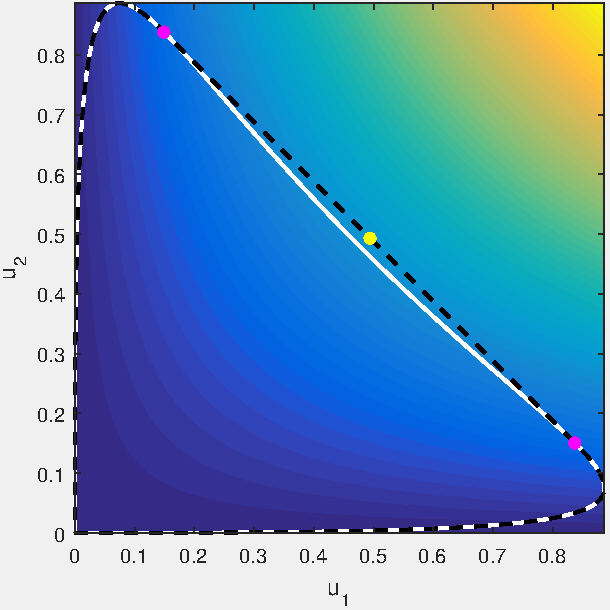
\includegraphics[width = \textwidth]{MixtureLikelihoods/GammaOptimHullSol}
			\subcaption{}\label{fig:GammaSol:subfig:Gamma}
		\end{minipage}
		\begin{minipage}{0.5\textwidth}
			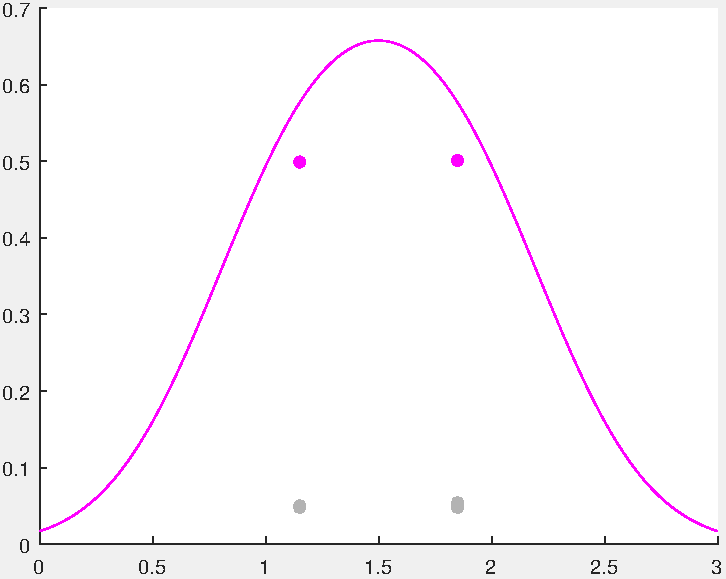
\includegraphics[width = \textwidth]{MixtureLikelihoods/MixingSolSigma045}				\subcaption{}\label{fig:GammaSol:subfig:Density}
		\end{minipage}
		\caption{In (\subref{fig:GammaSol:subfig:Gamma}), the boundary of $\conv(\Gamma)$ is shown as a dashed black line, $\Gamma$ is the white curve, the heat map  shows the objective function (likelihood increases from blue to yellow) and the yellow point is the maximizing point which can be written as the convex combination of the two magenta points. These two magenta points correspond to the two probability masses in the maximizing mixing distribution (\subref{fig:GammaSol:subfig:Density}).}
		\label{fig:GammaSol}
	\end{figure}
	The optimal point is on the boundary of $\conv(\Gamma)$ as expected and it can be written as the  $p_1 \vect{f}(\theta_1) + p_2 \vect{f}(\theta_2)$ (where $p_1 + p_2 =1 $). These two points correspond to the two probability masses in the maximizing mixture distribution shown in Figure \ref{fig:GammaSol:subfig:Density}. These masses are located at $\theta_1$ and $\theta_2$ with weights $p_1$ and $p_2$.

	\subsection{The effect of variance}
	In Figure \ref{fig:variance of ftheta}, we still use a normal density with mean $\theta$ as $f_\theta$ but we observe the effect that varying the variance, $\sigma^2$, has on the shape of $\Gamma$. We note that once $\sigma$ is large enough, the optimal point lies on $\Gamma$ and so only one point is needed in the maximum likelihood mixing distribution.
	\begin{figure}[ht]
		\centering
		\begin{minipage}{0.3\textwidth}
			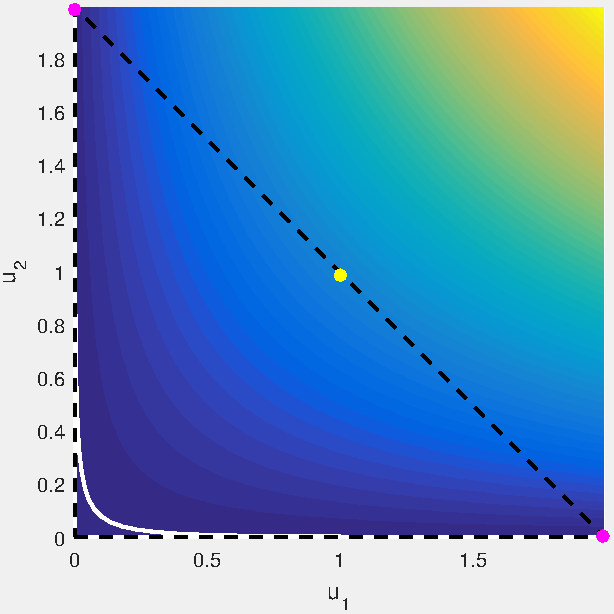
\includegraphics[width = \textwidth]{MixtureLikelihoods/GammaSigma02}
		\end{minipage}
		\begin{minipage}{0.3\textwidth}
			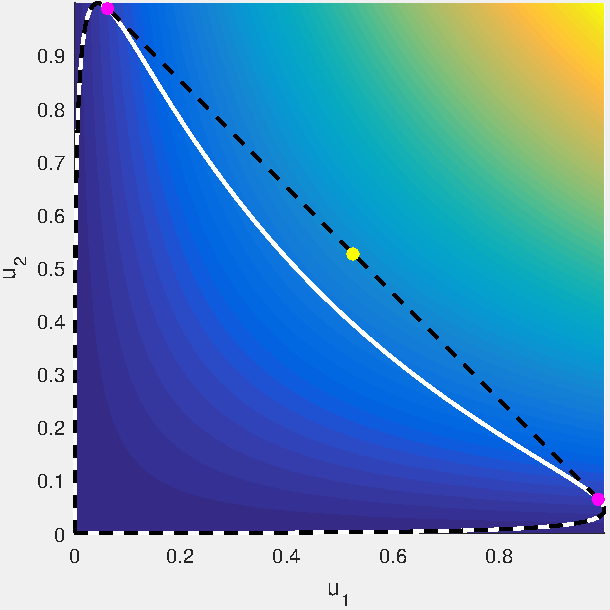
\includegraphics[width = \textwidth]{MixtureLikelihoods/GammaSigma04}
		\end{minipage}
		\begin{minipage}{0.3\textwidth}
			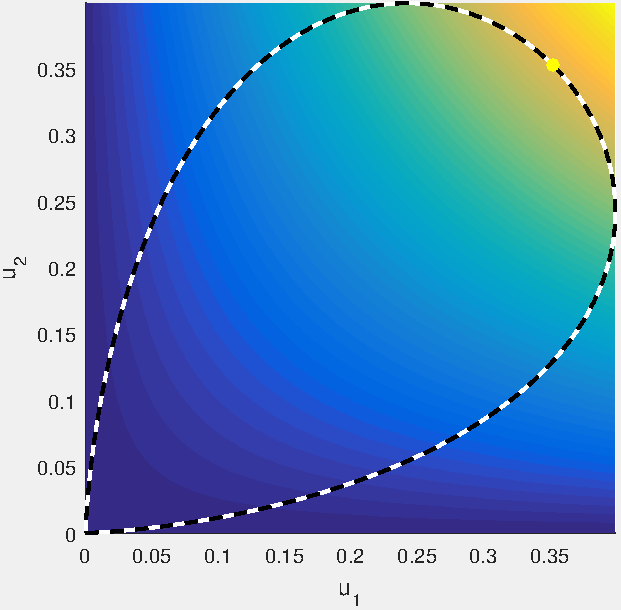
\includegraphics[width = \textwidth]{MixtureLikelihoods/GammaSigma1}
		\end{minipage}
		\begin{minipage}{0.3\textwidth}
			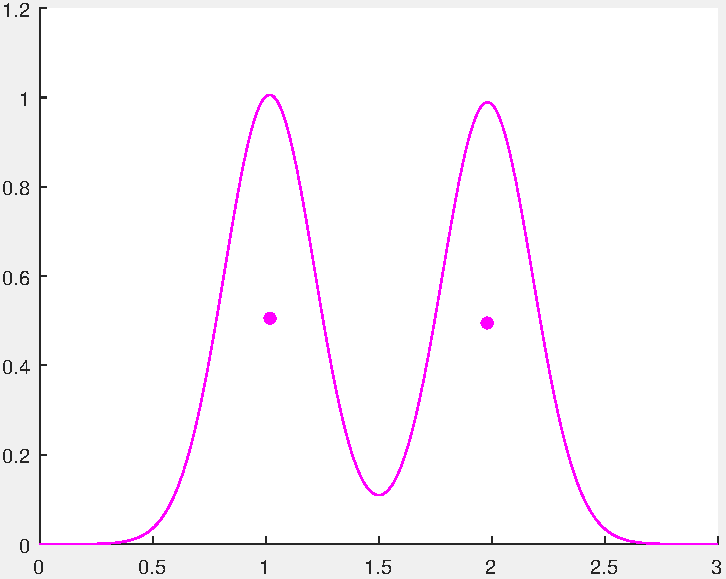
\includegraphics[width = \textwidth]{MixtureLikelihoods/MixingSolSigma02}
			\subcaption{$\sigma = 0.2$}
		\end{minipage}
		\begin{minipage}{0.3\textwidth}
			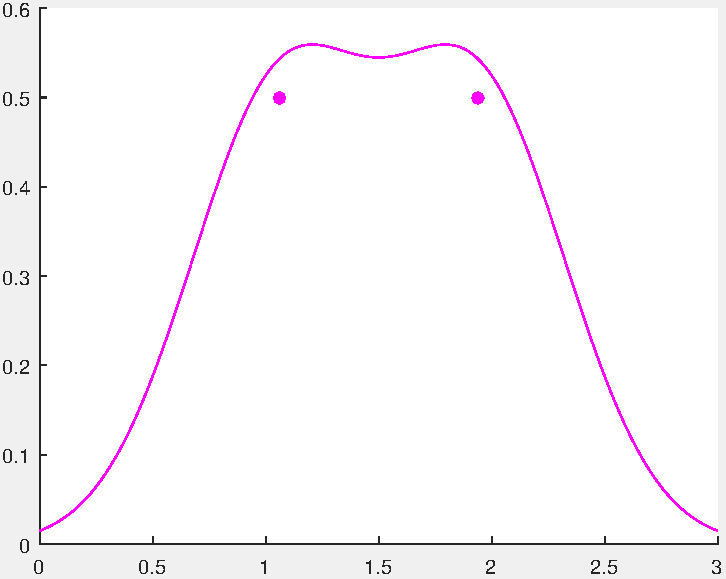
\includegraphics[width = \textwidth]{MixtureLikelihoods/MixingSolSigma04}
			\subcaption{$\sigma = 0.4$}
		\end{minipage}
		\begin{minipage}{0.3\textwidth}
			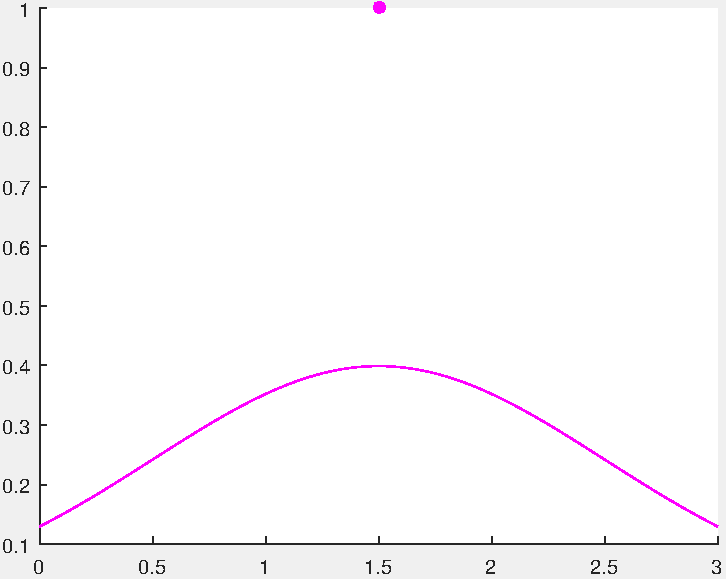
\includegraphics[width = \textwidth]{MixtureLikelihoods/MixingSolSigma1}
			\subcaption{$\sigma = 1$}
		\end{minipage}
		\caption{The maximum likelihood density for two points $X_1 = 1$ and $X_2 = 2$ where the component density, $f_\theta$, is a normal density with mean $\theta$ and variance $\sigma^2$. The variance is increased from left to right.}
		\label{fig:variance of ftheta}
	\end{figure}


	%\subsection{Critical value of $\sigma$}
		Figure \ref{fig:variance of ftheta} suggests that, for a fixed $X_1$ and $X_2$, there is a critical value of $\sigma$ at which the maximum likelihood mixing distribution, $Q$, goes from having two probability masses to having just one.
		
		\begin{theorem}
			If we have a sample with two points, $X_1$ and $X_2$, and we are finding the maximum likelihood mixture density for these points with 
			$$f_\theta(x) = \frac{1}{\sigma \sqrt{2\pi}} e^{-\frac{(x-\theta)^2}{2\sigma^2}}$$
			then a maximizing mixture distribution with only one probability mass exists if and only if
			$$|X_1 - X_2| \leq 2 \sigma$$
			\label{thm:distancebetweentwopoints}
		\end{theorem}
		We present two different proofs for this theorem.
		\begin{proof}[Proof 1]
			By stuff, if $|X_1 - X_2| \leq 2 \sigma$ then $\Gamma$ is convex and so optimal point must lie on $\Gamma$ and hence the corresponding maximizing mixture distribution has only one probability mass.
			If $|X_1 - X_2| > 2\sigma$ then just look at the picture... it's obvious... why do I have to make this so rigorous!?
		\end{proof}
		\begin{proof}[Proof 2]
			blah
		\end{proof}
	
\section{Differentiation of the log likelihood}
	This is from \cite{Lindsay1983-tf} but adapted for our context. We define the directional derivative of the likelihood from $Q_0$ to $Q_1$ to be
	$$\Phi(Q_1,Q_0) = \lim_{\epsilon \rightarrow 0} \epsilon^{-1} \left( L((1-\epsilon)Q_0 + \epsilon Q_1;\vect{y}) - L(Q_0;\vect{y}) \right).$$
	\begin{theorem}[Thm 4.1 from \cite{Lindsay1983-tf}]
		\label{thm:thm4point1}
		Let $\delta_\theta$ be the distribution that concentrates all of its mass at $\theta$. Then for any $Q$
		$$\sup_\theta \Phi(\delta_\theta,Q) \geq 0$$
		with equality if and only if $Q$ maximizes \eqref{eq:likelihood}.
	\end{theorem}

	\subsection{A strictly increasing sequence}
	%	We define a sequence $\{Q_j\}_{j=1}^n$ of discrete mixing distributions where
	%	$$Q_j = \argmax_{Q \text{ with no more than $j$ points of support}} L(Q;\vect{y})$$
	%	We define $\jmax = \argmax_j L(Q_j;\vect{y})$.

	Let $S_j$ be the set of all discrete mixing distributions with at most $j$ points of support. Consider the sequence $\{\alpha_j\}_{j=1}^n$ with
	\begin{equation}
	\alpha_j = \sup_{Q\in S_j} L(Q;\vect{y}).
	\label{eq:sequence}
	\end{equation}
	We know that this sequence must contain the maximum likelihood as there always exists a maximizing mixing distribution $\hat{Q}$ with no more than $n$ points of support. Let $\jmax$ be the smallest integer such that $\alpha_\jmax = L(\hat{Q})$. Clearly, $\alpha_\jmax = \alpha_{\jmax+1} = \dots = \alpha_n$.

	\begin{lemma} \label{lem:sequencestrictlyincreasing}
		The sequence $\{ \alpha_j\}_{j=1}^{\jmax}$ is strictly increasing.
	\end{lemma}
	\begin{proof}	
		
		It is not immediately clear whether or not we can replace the supremum in \eqref{eq:sequence} with a maximum. I'm pretty sure we can (I can't see how we could have a sequence of distributions in $S_j$ that converges to a distribution not in $S_j$) so let's just assume we can for now.
		
		Let $j < \jmax$ and choose some $Q_j \in S_j$ such that $\alpha_j = L(Q_j;\vect{y})$. From Theorem \ref{thm:thm4point1}, there exists some $\theta_0$ such that $\Phi(\delta_{\theta_0},Q_j) > 0$. Then for some $0<\epsilon <1$, $Q^* = (1-\epsilon)Q_j + \epsilon \delta_{\theta_0}$ satisfies $L(Q^*;\vect{y}) > L(Q_j;\vect{y})$. Now $Q^*$ has points of support at $\theta_0$ and at the points of support of $Q_j$. Hence $Q^*$ has no more than $j+1$ points of support. However, $Q^*$ must have more than $j$ points of support since $L(Q^*;\vect{y}) > \alpha_j$. So $Q^*$ has $j+1$ points of support and so $\alpha_{j+1} \geq L(Q^*;\vect{y}) > \alpha_j$.
		%This tells us that $\{\alpha_j\}_{j=1}^n$ is strictly increasing up to $\alpha_\jmax$ and is then constant.
	\end{proof}

\section{Additional Theorems about number of points}
	\begin{theorem}
		Given a sample $X_1,X_2,\dots,X_n$, define
		$$\epsilon = \min_{i \neq j}|X_i - X_j|.$$
		Define the density function
		$$f_\theta(x) = \begin{cases}
			1/\epsilon & \theta - \epsilon/2 < x < \theta + \epsilon/2\\
			0 &\text{otherwise.}
		\end{cases}$$
		Then there exists a discrete mixing distribution $Q$ with $n$ point masses that maximizes the likelihood
		$$\prod_{i = 1}^n \int_{-\infty}^{\infty} f_\theta(X_i) \intd Q(\theta)$$
	\end{theorem}
	\begin{proof}
		If $f_Q(X_i) = 0$ for any $i$ then $L(Q) = 0$. For any value of $\theta$, $f_\theta(x)$ is non-zero at no more than one $X_i$ and so $L(Q) > 0$ only for a $Q$ with at least $n$ point masses. By Theorem \ref{thm:LindsayGamma}, we need no more than $n$.
	\end{proof}
	\begin{theorem}
		Given a sample $X_1,X_2,\dots,X_n$, define
		$$E = \max_{i,j}|X_i - X_j|.$$
		Define the density function
		$$f_\theta(x) = \begin{cases}
		1/E & \theta - E/2 \leq x \leq \theta + E/2\\
		0 &\text{otherwise.}
		\end{cases}$$
		Then there exists a discrete mixing distribution $Q$ with 1 point mass that maximizes the likelihood
		$$L(Q) = \prod_{i = 1}^n \int_{-\infty}^{\infty} f_\theta(X_i) \intd Q(\theta)$$
	\end{theorem}
	\begin{proof}
		Consider the distribution $Q_0$ that puts a mass at $\theta_0 = (X_{max} - X_{min})/2$. The likelihood is $L(Q_0) = \left( \frac{1}{E} \right)^n$. Obviously the density at each $X_i$ is the maximum that it can possibly be and so $Q_0$ is a maximum likelihood mixing distribution.
	\end{proof}
	
	Remark: There is an important distinction when defining the density function as to whether you use $\leq$ or $<$. This feels a little strange.

%---results chapter---
% 2D simple results (minor extensions to Lindsay's results)
%	- 2 points, angle of trace results (difference between one and two points)
%	- Specific case of normal density?
% more general results 
%	- Numerical 'flag' graphs
%	- particular class of optimization problem
%	- constraints, gamma etc
%	- constraints for normals
%	- md result for normals
% %!TEX root = ..\..\main.tex
\chapter{Insights from Small \texorpdfstring{$n$}{n} Data}
\label{Ch:SmallNData}

\lhead{Chapter \ref{Ch:SmallNData}. \emph{Insights from Small \texorpdfstring{$n$}{n} Data}} % This is for the header on each page

%-------------------------------------------------------------------------------
%	Chapter Text
%-------------------------------------------------------------------------------

\section{Introduction}
	When we estimate the density of a random sample, $\vect{X} = X_1,X_2,\dots,X_n$, using a mixture model
	\begin{equation}
	f_Q(x) = \int_{-\infty}^{\infty} f_\theta(x) \intd Q(\theta)
	\end{equation}
	we often find that the mixing distribution, $Q$, that maximizes the log likelihood 
	\begin{equation}
	L(Q) = \sum_{i = 1}^n \log(f_Q(X_i))
	\label{smallndata:eq:likelihood}
	\end{equation}
	has only a few points of support. We can find insights into why this happens by looking at samples with small $n$. In this chapter we look in particular at the cases $n=2$ and $n=3$. Even though samples of this size are much smaller than those we would typically want to estimate the density of, the problem becomes significantly more simple (especially in the $n=2$ case) and some of the insights we gain can be applied to larger samples.

\section{Samples of size two}
	In section \ref{sec:mixturelikelihoods:geometrical}, we introduced the component likelihood vector 
	$$\vect{f}(\theta) = (f_\theta(X_1), \dots, f_\theta(X_n))$$
	and the set
	$$\Gamma = \{\vect{f}(\theta) : \theta \in \mathbb{R} \}.$$
	Now the analysis of $\Gamma$ is somewhat simplified when $\vect{f}(\theta)$ is two-dimensional (that is, $n = 2$)

\section{Phase Plots}
	We wish to make clear that the number of components in the MLE is purely a function of the data, $\vect{X} = (X_1, \dots, X_n)$. For any particular choice of $f_\theta$, we can think of the $n$ dimensional space of possible data sets as being partitioned by $C_k$, $k = 1,\dots,n$, where $C_k$ is the set of all $\vect{X}$ such that the MLE requires only $k$ components. The problem of determining the number of components required in the MLE for $\vect{X}$ becomes the problem of determining in which of the $C_k$ our data set lies for our choice of $f_\theta$.

	Let us consider the case where $f_\theta$ is normal with mean $\theta$ and variance $1$ and where $n=2$. From Theorem \ref{thm:distancebetweentwopoints},
	$$C_1 = \left \lbrace (X_1,X_2)\in \mathbb{R}^2 : |X_2 - X_1| \leq 2 \right\rbrace$$
	and so
	$$C_2 = \mathbb{R}^2 \setminus C_1.$$ We have plotted these two sets in Figure \ref{fig:phaseplotn2} for $-3<X_1,X_2<3$.
	\begin{figure}[ht]
		\centering
		\includegraphics[width=\textwidth]{SmallNData/Sigma1n2res256}
		\caption{title}
		\label{fig:phaseplotn2}
	\end{figure}

	We can produce similar plots for the three dimensional case ($n=3$) by fixing $x_1$ and letting $x_2$ and $x_3$ vary. In Figure \ref{fig:phaseplotn3}, we have used the same $f_\theta$, and set $x_1 = 0$. We should note that choosing a different value for $x_1$ would still result in the same plot, just transposed along the line $x_3 = x_2$. Additionally, choosing a different variance for $f_\theta$ would result in a plot with the same relative shape, but different scale.

	\begin{figure}[ht]
		\centering
		\includegraphics[width=\textwidth]{SmallNData/Sigma1n3res1024width7}
		\caption{title}
		\label{fig:phaseplotn3}
	\end{figure}

	In general, we expect that as our data gets closer together, the support of $Q$ gets smaller. However, Figure \ref{fig:phaseplotn3} demonstrates that this is not always the case.

	\subsection{The shape of \texorpdfstring{$C_1$}{C1} for normal densities}
	Here we present some bounds on $C_1$ when using a normal component density.

	\begin{theorem} \label{thm:shapeofC1normala}
		Let $f_\theta(x)$ be a normal density with mean $\theta$ and variance $\sigma^2$ and let $\vect{x} = (x_1,\dots,x_n)$ be the data for which we are finding a maximum likelihood density estimate. Write $\bar{x}$ for the mean of $\vect{x}$ and define $\vect{\bar{x}} = (\bar{x},\dots,\bar{x})$.
		
		Then $\vect{x} \notin C_1$ if
		$$|| \vect{x} - \vect{\bar{x}}|| > \sigma \sqrt{n}.$$
	\end{theorem}
	\begin{proof}
		We consider the function $L_2: \mathbb{R}^2 \mapsto \mathbb{R}$ where
		\begin{equation}\label{smallndata:eq:L2}
			L_2(\theta_1,\theta_2;p,\vect{x},\sigma) = \sum_{i = 1}^n \log\left[ \frac{1}{\sigma \sqrt{2 \pi}} \left( p \euler^{-(x_i - \theta_1)^2/2\sigma^2} + (1-p) \euler^{-(x_i - \theta_2)^2/2\sigma^2}\right) \right],
		\end{equation}
		$0<p<1$, $\sigma> 0$, $\vect{x} \in \mathbb{R}^n$.
		This is the log likelihood \eqref{smallndata:eq:likelihood} where $Q$ is restricted to having only two probability masses at locations $\theta_1$ and $\theta_2$ with probability masses $p$ and $1 - p$ respectively. 
		%Note that we treat the location of the masses as variables but think of the associated weights as fixed. 
	%	We do this since for any choice of $\theta_1 = \theta_2$, $L_2$ is constant along $p$. We intend to use derivatives to find stationary points of $L_2$ and then use second derivative tests to classify these points as either local maximums or not.
		
		If a sample, $\vect{x}$, lies in $C_1$ then for any $p$, $L_2(\theta_1,\theta_2;p,\vect{x},\sigma)$ attains its maximum value at some point where $\theta_1 = \theta_2$. Thus we are primarily interested in the stationary points of $L_2$ that occur along the line $\theta_1 = \theta_2$.
		
		Taking first derivatives of $L_2$ and setting $\theta_1 = \theta_2 = \theta$ we have
		\begin{equation}
		\left. \nabla L_2 \right|_{\theta_1 = \theta_2 = \theta} = \left(\frac{p}{\sigma^2} \sum_{i=1}^n(x_i - \theta),\frac{1-p}{\sigma^2} \sum_{i=1}^n(x_i - \theta)\right).
		\end{equation}
		This is zero only at $\theta = \bar{x}$. At this point, the Hessian matrix of $L_2$ is
		\begin{equation}
		H(\bar{x},\bar{x}) = \frac{1}{\sigma^4} \begin{pmatrix}
		-p n \sigma^2 + p(1-p) \sum_{i=1}^n (x_i - \bar{x})^2 &  -p(1-p) \sum_{i=1}^n (x_i - \bar{x})^2\\
		 -p(1-p) \sum_{i=1}^n (x_i - \bar{x})^2 & -(1-p) n \sigma^2 + p(1-p) \sum_{i=1}^n (x_i - \bar{x})^2
		\end{pmatrix}
		\end{equation}
		The determinant of this matrix is
		\begin{equation}
		|H(\bar{x},\bar{x})| = \frac{np(1-p)}{\sigma^6} \left(n\sigma^2 - \sum_{i=1}^n (x_i - \bar{x})^2 \right)
		\end{equation}
		which is negative for 
		\begin{equation}
		\sum_{i=1}^n (x_i - \bar{x})^2 > n \sigma^2,
		\end{equation}
		or equivalently
		\begin{equation}
		||\vect{x} - \vect{\bar{x}}|| > \sigma \sqrt{n}.
		\end{equation}
		
		Since a negative determinant corresponds to a saddle point, when $||\vect{x} - \vect{\bar{x}}|| > \sigma \sqrt{n}$, $L_2$ has no maximum along $\theta_1 = \theta_2$ and so $\vect{x} \notin C_1$.
	\end{proof}

	EXPAND ON SHAPE CYLINDER ETC

	This bound is shown for $n=3$ in Figure \ref{fig:C1bound}. We note that while it is necessary that $||\vect{x} - \vect{\bar{x}}|| \leq \sigma \sqrt{n}$ for $x$ to be in $C_1$, it is not sufficient. We will now adapt part of a theorem from \cite{Lindsay1983a-he} \cite{Lindsay1983a-he} to give us a sufficient condition for $\vect{x}$ to be in $C_1$.

	\begin{figure}[ht]
		\centering
		\includegraphics[width= \textwidth]{SmallNData/Sigma1n3res128width3_ellipse}
		\caption{text}
		\label{fig:C1bound}
	\end{figure}

	\begin{theorem}[\cite{Lindsay1983a-he}] \label{thm:shapeofC1normalb}
		Let $f_\theta(x)$ be a normal density with mean $\theta$ and variance $\sigma^2$ and let $\vect{x} = (x_1,\dots,x_n)$ be the data for which we are finding a maximum likelihood density estimate. Write $\bar{x}$ for the mean of $\vect{x}$. If the mixture quadratic
	%	$$\expect_\mu [(X - y_1)(X - y_K)]$$
		$$M(\theta) = (\theta - x_{(1)})(\theta - x_{(n)}) + \sigma^2$$
		is strictly positive on $[x_{(1)},x_{(n)}]$ then the mixing distribution with mass one at $\bar{x}$ must maximize the likelihood. 
	\end{theorem}
	\begin{corollary}
		If $x_{(n)} - x_{(1)} < 2\sigma$ then $\vect{x} \in C_1$.
	\end{corollary}

	SHOW BOUND in FIGURE

	\subsubsection{Probabilities}

	We now make the assumption that $\vect{x}$ is made up of i.i.d. random variables, $x_i$, which have distribution
	$$x_i \sim N(\mu,\sigma_1^2)$$
	for $i = 1,\dots,n$. Our component density, $f_\theta$, is normal with variance $\sigma_2^2$. From Theorem \ref{thm:shapeofC1normala},
	\begin{align*}
	p_u &= \prob \left( \sum_{i=1}^n (x_i - \bar{x})^2 \leq n \sigma_2^2  \right)
	\end{align*}
	is an upper bound to $\prob(\vect{x} \in C_1)$. Writing $s^2$ for the unbiased sample variance
	\begin{align*}
	p_u 
	%&= \prob\left( \frac{1}{n-1} \sum_{i=1}^n (x_i - \bar{x})^2 \leq \frac{n\sigma}{n-1}\right)\\
	&= \prob\left( s^2 \leq \frac{n \sigma_2^2}{n-1}\right)\\
	&= \prob\left( \frac{(n-1)s^2}{\sigma_1^2} \leq \frac{n \sigma_2^2}{\sigma_1^2}\right)\\
	&= \prob\left(\chi_{n-1}^2  \leq \frac{n \sigma_2^2}{\sigma_1^2} \right)
	\end{align*}
	where $\chi_{n-1}^2$ is chi-squared with $n-1$ degrees of freedom.

	From Theorem \ref{thm:shapeofC1normalb}, an lower bound to $\prob(\vect{x} \in C_1)$ is
	\begin{align*}
	p_l &= \prob(x_{(n)} - x_{(1)} < 2\sigma)\\
		&\geq \prob(\mu - \sigma < x_{(1)} < x_{(n)} < \mu + \sigma )\\
		&=  \left(\int_{\mu - \sigma}^{\mu + \sigma} f(x) \intd x \right)^n\\
		&= \left( \erf\left(\frac{\sigma_2}{\sqrt{2}\sigma_1}\right)\right)^n
	\end{align*}





	%%%%%% Conjecture turned out to be false so have removed this %%%%%%%
	%The proof of Theorem \ref{conj:shapeofC1normalb} will require the following lemma.	
	%\begin{lemma}
	%	A sample, $\vect{x}$, lies in $C_1$ if $L_2(\theta_1,\theta_2;p,\vect{x},\sigma)$ attains its maximum value at some point where $\theta_1 = \theta_2$.
	%\end{lemma}
	%\begin{proof}
	%	This is a Corollary of Lemma \ref{lem:sequencestrictlyincreasing}. If $\vect{x} \in C_k$ for some $k > 1$ then $\alpha_2 > \alpha_1$ and so $L_2(\theta_1,\theta_2;p,\vect{x},\sigma)$ cannot attain its maximum value at some point where $\theta_1 = \theta_2$.
	%\end{proof}

	%We are now ready to prove Theorem \ref{conj:shapeofC1normalb}.
	%\begin{conjecture} \label{conj:shapeofC1normalb}
	%	Let $f_\theta(x)$ be a normal density with mean $\theta$ and variance $\sigma^2$ and let $\vect{x} = (x_1,\dots,x_n)$ be the data for which we are finding a maximum likelihood density estimate. Write $\bar{x}$ for the mean of $\vect{x}$ and define $\vect{\bar{x}} = (\bar{x},\dots,\bar{x})$.
	%	
	%	Then $\vect{x} \in C_1$ if
	%	$$|| \vect{x} - \vect{\bar{x}}|| \leq \sigma \sqrt{n}.$$
	%\end{conjecture}
	%\begin{proof}
	%	We know that $(\bar{x},\bar{x})$ is a local maximum of $L_2(\theta_1,\theta_2;p,\vect{x},\sigma)$ when
	%	$$|| \vect{x} - \vect{\bar{x}}|| < \sigma \sqrt{n}.$$
	%	
	%	Sufficient to show that no other stationary points exist in this case (as local max must exist).
	%	
	%	Sufficient to show that only one local maximum exists
	%	
	%	Idea: some sort of polar coordinates around $(\bar{x},\bar{x})$.
	%	
	%	Use directional derivative to show only one maximum exists (up to symmetry)... no idea how though :P Actually not true for some symmetrical data...I think...
	%	
	%	At local max, what is directional derivative in any direction? If it's negative/0 then at global max...
	%	
	%	Read Lindsay. Lemma should be something like local maximum is global maximum.
	%	Hold on - but definitely not at global max at saddle point so what's happening?
		
	%	We observe that if
	%	\begin{equation}
	%	\sum_{i=1}^n (x_i - \bar{x}) < n \sigma^2,
	%	\end{equation}
	%	then 
	%	\begin{equation}
	%	\frac{\partial^2 L_2}{\partial \theta_1^2} (\bar{x},\bar{x}) = \frac{1}{\sigma^4} \left( -p n \sigma^2 + p(1-p) \sum_{i=1}^n (x_i - \bar{x})^2 \right) < 0.
	%	\end{equation}
	%	So when $||\vect{x} - \vect{\bar{x}}|| < \sigma \sqrt{n}$, the point $(\bar{x},\bar{x})$ is a local maximum of $L$.
	%	
	%	We need to show that it is a global maximum. Lemma?
	%	
	%	It remains to determine the boundary case. Lemma?
	%\end{proof}


	%\subsection{Normal with one component}
	%
	%%obviously add in real formula for normal later
	%Consider the problem where we restrict $Q$ to concentrating all of its mass at one point, $\phi$, and where our component density, $f_\theta(x)$, is normal with mean $\theta$ and variance $\sigma$. Then we can write the log likelihood as
	%\begin{align*}
	%L(\phi;\vect{x}) &= \sum_{i=1}^n \log \left(\frac{1}{2\sigma} e^{-(x_i - \phi)^2/\sigma^2}\right)\\
	%&= -n\log(2\sigma) - \frac{1}{\sigma^2}\sum_{i = 1}^n (x_i - \phi)^2
	%\end{align*}
	%In order to maximize this we need to choose $\phi$ to minimize
	%\begin{equation}
	%\sum_{i=1}^n (x_i - \phi)^2.
	%\label{eq:sumofsquares}
	%\end{equation}
	%If we write $\vect{\Phi}(\phi) = \{\phi,\dots,\phi\}$ then the $\phi$ that minimizes \eqref{eq:sumofsquares} is the $\phi$ that minimizes the Euclidean distance between $\vect{x}$ and $\vect{\Phi}(\phi)$. %We note that $\min_\phi(L(\phi ;\vect{x}))$ is a function of the distance between $\vect{x}$ and the line $x_1 = x_2 = \dots = x_n$.
	%
	%%Speculative
	%
	%We now consider the case where $Q$ has $2$ points of mass, $p_j$ at $\phi_j$ for $j = 1,...,m$. The log likelihood can be written as
	%\begin{align*}
	%L(Q;\vect{x}) &= \sum_{i=1}^n \log \left( \frac{1}{2\sigma} \sum_{j = 1}^2 p_j e^{(-x_i - \phi_j)^2/\sigma^2}\right)\\
	%&=-n\log(2\sigma) + \sum_{i=1}^n \log\left(\sum_{j=1}^2 p_j e^{(-x_i - \phi_j)^2/\sigma^2} \right)\\
	%&=-n\log(2\sigma) + \sum_{i=1}^n \log\left(p_1 e^{-(x_i - \phi_1)^2/\sigma^2} + p_2 e^{(-x_i - \phi_2)^2/\sigma^2} \right)\\
	%%&=-n\log(2\sigma) +\sum_{i = 1}^n \log\left(p_1 e^{-(x_i - \phi_1)^2/\sigma^2}\right) + \sum_{i=1}^n \log \left(1+ \frac{p_2}{p_1}\frac{e^{-(x_i - \phi_2)^2/\sigma^2}}{e^{-(x_i - \phi_1)^2/\sigma^2}} \right)\\
	%%&= -n\log(2\sigma) - \frac{1}{\sigma^2} \sum_{i=1}^n (x_i - \phi_1)^2 + n\log(p_1) + \sum_{i=1}^n \log \left(1+ \frac{p_2}{p_1} e^{((x_i - \phi_1)^2 -(x_i - \phi_2)^2)/\sigma^2} \right)
	%\end{align*}

	%	We now consider the case where $Q$ has $m$ points of mass, $p_j$ at $\phi_j$ for $j = 1,...,m$. The likelihood can be written as
	%	\begin{align*}
	%	L(Q;\vect{x}) &= \sum_{i=1}^n \log \left( \frac{1}{2\sigma} \sum_{j = 1}^m p_j e^{(-x_i - \phi_j)^2/\sigma^2}\right)\\
	%		&=-n\log(2\sigma) + \sum_{i=1}^n \log\left(\sum_{j=1}^m p_j e^{(-x_i - \phi_j)^2/\sigma^2} \right)\\
	%		&=-n\log(2\sigma) + \sum_{i=1}^n \log\left(p_1 e^{-(x_i - \phi_1)^2/\sigma^2} + \sum_{j=2}^m p_j e^{(-x_i - \phi_j)^2/\sigma^2} \right)\\
	%		&=-n\log(2\sigma) +\sum_{i = 1}^n \log\left(p_1 e^{-(x_i - \phi_1)^2/\sigma^2}\right) + \sum_{i=1}^n \log \left(1+ \sum_{j=2}^m \frac{ p_j e^{(-x_i - \phi_j)^2/\sigma^2}}{p_1 e^{-(x_i - \phi_1)^2/\sigma^2}} \right)\\
	%		&= -n\log(2\sigma) - \frac{1}{\sigma^2} \sum_{i=1}^n (x_i - \phi_1)^2 + n\log(p_1) + \sum_{i=1}^n \log \left(1+ \sum_{j=2}^m \frac{ p_j e^{(-x_i - \phi_j)^2/\sigma^2}}{p_1 e^{-(x_i - \phi_1)^2/\sigma^2}} \right)
	%	\end{align*}

	%For $\sigma = 1$ this has partial derivatives
	%\begin{align*}
	%\frac{\partial L}{\partial \phi_1} &= -2 p_1 \sum_{i=1}^n  \frac{(\phi_1 - x_i) e^{-(\phi_1 - x_i)^2}}{p_1 e^{-(x_i - \phi_1)^2} + p_2 e^{(-x_i - \phi_2)^2}}\\
	%\frac{\partial L}{\partial \phi_2} &= -2 p_2 \sum_{i=1}^n  \frac{(\phi_2 - x_i) e^{-(\phi_2 - x_i)^2}}{p_1 e^{-(x_i - \phi_1)^2} + p_2 e^{(-x_i - \phi_2)^2}}\\
	%\frac{\partial L}{\partial p_1} &=  \sum_{i=1}^n  \frac{e^{-(\phi_1 - x_i)^2} - e^{-(\phi_2 - x_i)^2}}{p_1 e^{-(x_i - \phi_1)^2} + (1-p_1) e^{(-x_i - \phi_2)^2}}\\
	%\frac{\partial^2 L}{\partial \phi_1^2} &= -2p_1\sum_{i=1}^n \frac{2p_1 (\phi_1-x_i)^2 e^{-2(\phi_1 - x_i)^2}}{(p_1 e^{-(x_i - \phi_1)^2} + p_2 e^{-(x_i - \phi_2)^2})^2} + 
	%\frac{e^{-(\phi_1 - x_i)^2}(1 -2 (\phi_1 - x_i)^2)}{p_1 e^{-(x_i - \phi_1)^2} + p_2 e^{-(x_i - \phi_2)^2}}\\
	%\frac{\partial^2 L}{\partial \phi_2^2} &= -2p_2\sum_{i=1}^n \frac{2p_2 (\phi_2-x_i)^2 e^{-2(\phi_2 - x_i)^2}}{(p_1 e^{-(x_i - \phi_1)^2} + p_2 e^{-(x_i - \phi_2)^2})^2} + 
	%\frac{e^{-(\phi_2 - x_i)^2}(1 -2 (\phi_2 - x_i)^2)}{p_1 e^{-(x_i - \phi_1)^2} + p_2 e^{-(x_i - \phi_2)^2}}\\
	%\frac{\partial^2 L}{\partial p_1^2} &=  -\sum_{i=1}^n  \frac{\left( e^{-(\phi_1 - x_i)^2} - e^{-(\phi_2 - x_i)^2}\right)^2}{\left(p_1 e^{-(x_i - \phi_1)^2} + (1-p_1) e^{(-x_i - \phi_2)^2}\right)^2}\\
	%\frac{\partial^2 L}{\partial \phi_1 \partial \phi_2} &= -4 p_1 p_2 \sum_{i=1}^n  \frac{(\phi_1 - x_i)(\phi_2 - x_i) e^{-(\phi_1 - x_i)^2-(\phi_2 - x_i)^2}}{(p_1 e^{-(x_i - \phi_1)^2} + p_2 e^{-(x_i - \phi_2)^2})^2}\\
	%\frac{\partial^2 L}{\partial p_1 \partial \phi_1} &= -2 \sum_{i=1}^n \frac{(\phi_1 - x)e^{}}{}\\
	%\frac{\partial^2 L}{\partial p_1 \partial \phi_2} &= -2 \sum_{i=1}^n
	%\end{align*}
	%
	%at $\phi_1 = \phi_2 = \phi$ these are
	%
	%\begin{align*}
	%\left. \frac{\partial L}{\partial \phi_1} \right\rvert_{\phi_1,\phi_2 = \phi} &= -2 p_1 \sum_{i=1}^n  (\phi - x_i)\\
	%\left.\frac{\partial L}{\partial \phi_2}\right\rvert_{\phi_1, \phi_2 = \phi}  &= -2 p_2 \sum_{i=1}^n  (\phi - x_i)\\
	%\left.\frac{\partial^2 L}{\partial \phi^2}\right\rvert_{\phi_1, \phi_2 = \phi}  &= n + 4p_1p_2\sum_{i=1}^n (\phi-x_i)^2\\
	%\left.\frac{\partial^2 L}{\partial \phi_1 \partial \phi_2}\right\rvert_{\phi_1,\phi_2 = \phi}  &= -4 p_1 p_2 \sum_{i=1}^n (\phi - x_i)^2\\
	%\left.\frac{\partial^2 L}{\partial \phi_2^2}\right\rvert_{\phi_1, \phi_2 = \phi}  &= n + 4p_1p_2\sum_{i=1}^n  (\phi-x_i)^2
	%\end{align*}
	%
	%\begin{equation}
	%D = \left(n+4p_1p_2\sum_{i=1}^n (\phi - x_i)^2\right)^2 - \left(4p_1p_2\sum_{i=1}^n (\phi - x_i)^2\right)^2>0
	%\end{equation}
	%and
	%\begin{equation}
	%\frac{\partial^2 L}{\partial \phi^2} > 0
	%\end{equation}
	%
	%so $\phi_1 = \phi_2 = \phi$ is local minimum.
	%
	%At $\phi_1 = \phi_2 = \phi$ the Hessian Matrix is
	%\begin{equation}
	%H = 
	%\begin{pmatrix}
	%n+4p_1p_2\sum_{i = 1}^n (\phi-x_i)^2 & -4 p_1 p_2 \sum_{i=1}^n (\phi - x_i)^2 & -2\sum_{i=1}^n (\phi - x_i)\\
	%-4 p_1 p_2 \sum_{i=1}^n (\phi - x_i)^2& n + 4p_1p_2\sum_{i=1}^n  (\phi-x_i)^2 & 2\sum_{i=1}^n (\phi - x_i)\\
	%-2\sum_{i=1}^n (\phi - x_i)& 2\sum_{i=1}^n (\phi - x_i)& 0
	%\end{pmatrix}
	%\end{equation}
	%
	%This is a Hermitian matrix and so we can use Sylvester's criterion to determine when it is positive definite.
	%
	%Clearly
	%\begin{equation}
	%n+4p_1p_2\sum_{i = 1}^n (\phi-x_i)^2
	%\end{equation}
	%is positive and
	%\begin{equation}
	%\begin{pmatrix}
	%n+4p_1p_2\sum_{i = 1}^n (\phi-x_i)^2 & -4 p_1 p_2 \sum_{i=1}^n (\phi - x_i)^2\\
	%-4 p_1 p_2 \sum_{i=1}^n (\phi - x_i)^2& n + 4p_1p_2\sum_{i=1}^n  (\phi-x_i)^2
	%\end{pmatrix}
	%\end{equation}
	%has positive determinant.
	%
	%However,
	%\begin{equation}
	%\det(H) = -8n \left(\sum_{i=1}^n (x_i - \phi) \right)^2
	%\end{equation}
	%which is negative. So the second derivative test is inconclusive.

	%%%%%Extra stuff that doesn't quite fit in yet%%%%%{}
% %!TEX root = ..\main.tex
\chapter{A Particular Class of Optimization Problem}
\label{Ch:StatOptim}

\lhead{Chapter \ref{Ch:StatOptim}. \emph{A Particular Class of Optimization 
Problem}} % This is for the header on each page

\section{Introduction}

"The results follow from this general theorem which seems obvious."

\begin{theorem}
	Let $(E_m)_{m=1}^\infty$ be a sequence of appropriately defined sets and let
	$(g_m)_{m=1}^\infty, g_m: E_m \mapsto \mathbb{R}$ be a sequence of
	functions that satisfy the following properties
	\begin{enumerate}
		\item $\forall \vect{x} \in \partial E_m, \exists n < m, \vect{y} \in E_n$ such that
		$g_m(\vect{x}) \leq g_n(\vect{y})$.
		\label{prop:one}
		\item $\exists m_0, \vect{x}_0 \in E_{m_0}$ such that $\forall m, \vect{x} \in 
		E_m$, $g_m(\vect{x}) \leq g_{m_0}(\vect{x}_0)$.
	\end{enumerate}
	Then $\exists m_*, \vect{x}_* \in E_{m_*} \setminus \partial E_{m_*}$ such
	that $\forall m, \vect{x} \in E_m$, $g_m(\vect{x}) \leq g_{m_*}(\vect{x}_*)$.
\end{theorem}
\proof{
	The proof is simple. If $\vect{x}_0 \notin \partial E_{m_0}$ then we are done.
	Otherwise, by property \ref{prop:one} we can find a $n$ and $\vect{y} \in 
	E_n$ such that $g_n(y) = g_{m_0}(\vect{x}_0)$. If $\vect{y} \notin \partial 
	E_n$ then we are done, otherwise we repeat the process until we find a $m, 
	\vect{x}$ pair with $\vect{x} \notin \partial E_m$. %Note that property 
	% \ref{prop:one} implies that $\partial E_1 = \emptyset$ and so this process
	% must end.
}



% Given a sequence of functions $(g_m)_{m=1}^\infty $, $g_m: \mathbb{R}^{m} \times 
% \mathbb{R}^m \mapsto \mathbb{R}$, find the $m$, $\vect{p} = (p_1, \dots, p_m)$ 
% and $\vect{\theta} = (\theta_1, \dots, \theta_m)$ that maximize
% \begin{equation}
% 	g_m\left( \vect{p}, \vect{\theta}	\right)
% 	\label{eq:objective}
% \end{equation}
% subject to
% \begin{align}
% 	p_j &\geq 0, \label{eq:constraint1}\\
% 	\sum_{j=1}^m p_j &= 1,\label{eq:constraint2}\\
% 	\theta_j &\leq \theta_{j+1} \label{eq:constraint3}
% \end{align}
% where the $g_m$ satisfies the following properties.

% \begin{align}
% 	g_m(p_1, \dots, p_{i-1}, 0, p_{i+1}, \dots, p_m, \vect{\theta}) 
% 		&= g_{m-1}(p_1, \dots, p_{i-1}, p_{i+1}, \dots, p_m, \theta_1, \dots,
% 		\theta_{i-1}, \theta_{i+1}, \dots, \theta_m)\\
% 		&= 
% \end{align}

% It will often prove more convenient for us to consider the equivalent problem 
% obtained by using \eqref{eq:constraint2} to eliminate $p_m$:

% Given functions $\vect{g}: \mathbb{R} \mapsto \mathbb{R}^n$, $h: \mathbb{R}^n 
% \mapsto \mathbb{R}$ and $m \in \mathbb{N^+}$, find the $\vect{p} = 
% (p_1, \dots, p_{m-1})$ and $\vect{\theta} = (\theta_1, \dots, \theta_m)$ that 
% maximize
% \begin{equation}
% 	h\left( \sum_{j=1}^{m-1} p_j \vect{g}(\theta_j) +
% 	\left(1 - \sum_{j=1}^{m-1} p_j \right) \vect{g}(\theta_m)
% 	\right)
% 	\label{eq:objective_alt}
% \end{equation}
% subject to
% \begin{align}
% 	p_j &\geq 0, \label{eq:constraint1_alt}\\
% 	\sum_{j=1}^{m-1} p_j &\leq 1,\label{eq:constraint2_alt}\\
% 	\theta_j &\leq \theta_{j+1}. \label{eq:constraint3_alt}
% \end{align}


% We make the following observation.
% \begin{theorem}
% 	If \eqref{eq:objective_alt} has a boundary solution ($p_i = 0$ or 
% 	$\theta_i = \theta_{i+1}$) for $m = M$, then there exists an $M^* < M$ such 
% 	that \eqref{eq:objective_alt} has an interior solution with the same value 
% 	for $m = M^*$.
% 	\label{thm:exists_interior_solution}
% \end{theorem}
% \begin{remark}
% 	If $g$ and $h$ are differentiable, then at an interior solution, all
% 	derivatives of our objective function are equal to zero.
% \end{remark}

% \begin{theorem}
% 	Max is always $m \leq n$??
% \end{theorem}

% \subsection{Examples}
% One problem that takes this form is that of finding a maximum likelihood
% mixture. Given data $\vect{x} = (x_1, \dots, x_n)$, and a component density
% $f(x; \theta)$, set 
% \begin{equation}
% 	\vect{g}(\theta) = (f(x_1; \theta), \dots, f(x_n; \theta))
% \end{equation}
% and
% \begin{equation}
% 	h(g_1, \dots, g_n) = \sum_{i = 1}^n \log(g_i).
% \end{equation}

\section{Maximum Likelihood Location Mixtures of Normals}


%--- Mixture chapter---
%!TEX root = ..\..\main.tex
\chapter{Maximum Likelihood Location Mixtures}
\label{Ch:Mixtures}

\lhead{Chapter \ref{Ch:Mixtures}. \emph{Maximum Likelihood Location Mixtures}}

\graphicspath{{Figures/Mixtures/}}

%-------------------------------------------------------------------------------
%	Chapter Text
%-------------------------------------------------------------------------------

\section{Introduction}
	Mixtures of distributions have been used to model a wide variety of phenomena, with successful applications in the fields of ``astronomy, biology, genetics, medicine, psychiatry, economics, engineering, and marketing, among many other fields in the biological, physical, and social sciences'' \cite[Section 1.1.1]{McLachlan2004-ik}. Mixture models have been in use for over 100 years. In 1894, Pearson used a mixture of two normal densities to model the distribution of the ratio of forehead to body lengths of a sample of 1000 crabs \cite{Pearson1894-qv}. His mixture of two normals was able to account for the skewness in the data, which a single normal could not model. Pearson suggested that this signalled the existence of two sub-populations of crabs; each associated with its own normal distribution.

	However, we do not require that data comes from a mixture of distributions in any physical sense for mixtures to be a useful modelling tool. 
	One of the traits that has contributed to the extent of the use of mixtures is that they provide a convenient semi-parametric way of modelling unknown distributions. They are particularly useful in situations where a parametric method is too restrictive to satisfactorily model the data, and a fully non-parametric method, such as kernel density estimation, may require evaluating a sum which contains more terms than desired. By way of illustration, Priebe in \cite{Priebe1994-ng} discussed modelling a log normal density using a mixture of normals. With $n = 10000$ observations, Priebe only required about 30 normals to obtain a good approximation. This is in contrast to a kernel density estimator which would contain 10000 terms.

	% [WHAT ELSE?]

	% \subsection{Definitions}
	A \emph{mixture density} is a probability density function that can be written in the form
	\begin{equation}
		f_Q(\vect{x}) = \int_\Omega f(\vect{x}; \vect{\theta}) \intd Q(\vect{\theta}),
		\label{eq:mixture definition}
	\end{equation}
	where $f(\vect{x};\vect{\theta})$ is the \emph{component density}, parametrised by $\vect{\theta} \in \Omega$, and $Q$ is a probability distribution on $\Omega$, called the \emph{mixing distribution}. In the case that $Q$ is a discrete probability distribution, with probability masses $p_j$ at points $\vect{\theta}_j$, $j = 1, \dots, m$, the mixture density in \eqref{eq:mixture definition} is a \emph{finite mixture} and can be written
	\begin{equation}
		f_Q(\vect{x}) = f_{\vect{\theta}, \vect{p}}(\vect{x}) = \sum_{j = 1}^m p_j f(\vect{x}; \vect{\theta}_j).
	\end{equation}

	In this chapter, we will be concerned only with finite mixtures on the real line, whose component densities are parametrised by a single shifting parameter, $\theta$ (we may of course allow for other fixed parameters, for example normal distributions with varying locations but fixed variance). This is what we will call a \emph{location mixture}, and it can be written as
	\begin{equation}
		f_{\vect{p}, \vect{\theta}} = \sum_{j = 1}^m p_j f(x - \theta_j)
		\label{eq:location mixture}
	\end{equation}
	for a single component density $f(x)$.
	Looking only at mixtures of this form is not as restrictive as it may at first seem. Using a finite location mixture of normals, one can approximate any continuous density arbitrarily well \cite{Nguyen2018-qx}.

	A common question when using mixtures is the following. Let $\vect{X} = (X_1, \dots, X_n)$ be a set of independent and identically distributed random variables, where each $X_i$ has probability density function $g(\vect{x})$. Given $\vect{x} = (x_1, \dots, x_n)$, an observed random sample of $\vect{X}$, and a component density $f(\vect{x}; \vect{\theta})$, how do we choose the mixing distribution $Q$ so that $f_Q(\vect{x})$ is a good approximation for $g(\vect{x})$?	One answer to this question is to choose $Q$ to maximise the likelihood.

	The \emph{likelihood} of a distribution $Q$ given $\vect{x}$ is 
	\begin{equation}
		L(Q;\vect{x}, f) = \prod_{i = 1}^n f_Q(x_i).
	\end{equation}
	Maximizing $L(Q;\vect{x}, f)$ may be achieved by instead maximizing the \emph{log likelihood},
	\begin{equation}
		l(Q; \vect{x}, f) = \log L(Q; \vect{x}, f) = \sum_{i = 1}^n \log f_Q(x_i),
		\label{eq:loglikelihood}
	\end{equation}
	since $\log(x)$ is a strictly increasing function. In \cite{Lindsay1983-tf}, Lindsay showed that provided that the likelihood is bounded, there exists a maximizing $Q$ that has at most $n$ points of support. This is a useful result because it means that the problem of finding a maximizing $Q$ is an optimization problem having finite dimensions. It also justifies our decision to consider only finite mixtures in this chapter.

	However, we often find that the maximizing $Q$ has far fewer than $n$ points of support. An example of this is shown in Figure \ref{fig:chi2 n500 motivation}. In this example we have taken $n = 500$ points from a chi-squared distribution with 3 degrees of freedom and used a normal component density with fixed variance $\sigma^2 = 1$ as our component density. The maximum likelihood mixing distribution $Q$ has only 6 points of support (represented by points $(\theta_j, p_j)$ for each probability mass $p_j$ at $\theta_j$), well short of the stated bound of $500$. This behaviour is typical for maximum likelihood location mixtures, with the upper bound of $n$ only being realised in pathological cases where the observations are spread widely apart.

	\begin{figure}
		\centering
		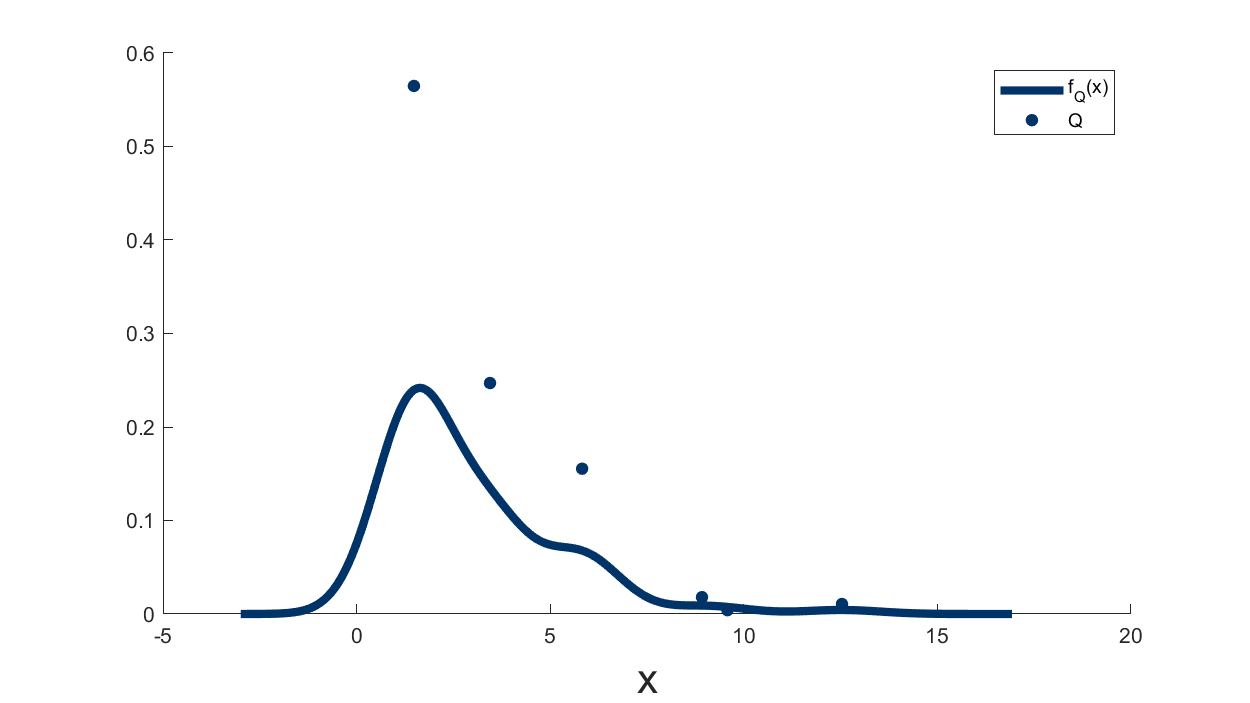
\includegraphics[width = \textwidth]{Figures/Mixtures/chi2_n500_motivation.png}
		\caption{A maximum likelihood location mixture of $n = 500$ points where the maximising mixing distribution, $Q$, has only 6 points of support.}
		\label{fig:chi2 n500 motivation}
	\end{figure}

	% While one can construct examples in which the mixing distribution that maximizes the likelihood has all $n$ points of support, in practise, 
	The size of the support of the $Q$ that maximizes \eqref{eq:loglikelihood} is the primary quantity of interest for this chapter. We define it as follows. Let $\mathcal{Q}_n$ be the set of all discrete probability distributions on $\mathbb{R}$ with no more than $n$ points of support. Let
	\begin{equation}
		\hat{Q}_{\vect{x},f} = \{Q \in \mathcal{Q}_n: l(Q;\vect{x},f) \geq l(Q';\vect{x},f), \forall Q' \in \mathcal{Q}_n\}
	\end{equation}
	be the set of all global maximizers of \eqref{eq:loglikelihood}. Then define
	\begin{equation}
		K_\vect{x} = K(\vect{x}; f) = \min\{m : \mathcal{Q}_m \cap \hat{Q}_{\vect{x},f} \neq \emptyset\}
		\label{eq:K_x definition}
	\end{equation}
	which counts the smallest number of probability masses needed to maximize the likelihood.


	There are a few considerations to be made here. The first is that there is not necessarily a unique mixing distribution that maximizes \eqref{eq:loglikelihood} and so we have defined the quantity of interest as the smallest number of points of support required for a maximizing distribution. However, in many cases, including when the component density is from the exponential family, we know that the maximizing mixing distribution is unique. This question of uniqueness was addressed by Lindsay in \cite{Lindsay1983-tf} and in \cite{Lindsay1983a-he} for continuous univariate component densities in the exponential family. A generalization of these results to discrete exponential families can be found in \cite{Lindsay1993-rj}.

	The second, is that our choice to consider only location mixtures is significant in that it guarantees that the likelihood is bounded so long as the component density is bounded. In general, this is not the case. Consider the likelihood function for a mixture of normals parametrized by both the mean and variance. We can create a mixture by placing equally weighted normals with very small variance at each $x_i$ in our sample. This corresponds to a mixing distribution $Q$ which places probability mass $1/n$ at points $(x_i, \sigma^2)$ for $i = 1, \dots, n$. As $\sigma^2$ approaches zero, the density at each $x_i$, $f_Q(x_i)$, increases without bound and so the likelihood is unbounded. There are a number of techniques that can be employed to ensure the likelihood is bounded such as restricting the parameter space appropriately or restricting the number of components to some number that grows slowly with $n$ (the sieve method \cite{Grenander1981-dy}).

	The third, is that we should be careful to make a distinction between calculating $K_\vect{x}$ and choosing an appropriate number of components for a mixture model. The former is simply a deterministic property of an optimization problem whereas the latter is an in-depth and difficult problem which involves consideration of properties such as consistency, and the use of techniques such as information criteria and likelihood ratio. This latter problem is discussed in \cite[Chapter 6]{McLachlan2004-ik}. In particular, if each $X_i$ comes from a distribution with density $g(x) = f_Q(x)$ (that is, $g(x)$ is a mixture density itself) then we may consider the `true' number of components and using certain penalised log likelihood criteria, such as the Akaike information criterion (AIC) \cite{Akaike1974-bl} or the Bayesian information criterion (BIC) \cite{Schwarz1978-ci}, does not underestimate this quantity asymptotically \cite{Leroux1992-ek}. This suggests that we should not expect $K_\vect{x}$ (which is defined from an unpenalised likelihood) to necessarily be reflective of the properties of $g(x)$.
 
	% Not necessarily unique Q
	% Location mixtures only (otherwise unbounded likelihood and use all n points)
	% Mention sieves
	% NOT about recovering the 'true' number of components - we are using mixtures as a density approximation tool and are interested in the property of this optimization.

	% A location mixture on $\mathbb{R}$ with mixing distribution $Q$ and component density $f(x)$ can be written as
	% \begin{equation}
	% 	f_Q(x) = \int_{-\infty}^\infty f(x-\theta) \intd Q(\theta).
	% \label{eq:mixtureint}
	% \end{equation}

	% Given a sample $\vect{x} = (x_1,\dots,x_n)$, we wish to find a distribution that maximizes the log likelihood	
	% \begin{equation}
	% 	L(Q;\vect{x}) = \sum_{i = 1}^n \log(f_Q(x_i)).
	% \label{eq:loglikelihood}
	% \end{equation}
	% Lindsay showed that under quite general conditions, such a maximizing distribution exists and has no more than $n$ points of support \cite{Lindsay1983-tf}. It is therefore common to use
	% \begin{equation}
	% 	f_{\vect{p},\vect{\theta}}(x) = \sum_{j = 1}^m p_j f(x - \theta_j)
	% \label{eq:mixturesum}
	% \end{equation}
	% instead of \eqref{eq:mixtureint} as our definition of a location mixture. We note that \eqref{eq:mixtureint} is equivalent to \eqref{eq:mixturesum} in the case where $Q$ is a discrete distribution which places probability masses of weight $p_j$ at locations $\theta_j$, for $j = 1,\dots,m$. The order of the $x_i$ does not matter and so we will assume without loss of generality that $x_1 \leq x_2 \leq \dots \leq x_n$ throughout.
	
	% In this paper we are primarily interested in the number of probability masses that are required in the maximizing mixture. We will call this quantity $K_{\vect{x}}$. It should be noted that there is not always a unique mixing distribution that maximizes \eqref{eq:loglikelihood}. However we can choose $K_{\vect{x}}$ to be the smallest number of probability masses that any of the maximizing distributions have.
\section{Summary of Lindsay}
\label{sec:summary of Lindsay}

	To obtain results concerning $K_\vect{x}$ we will make use of the geometric approach employed by Lindsay in \cite{Lindsay1983-tf} and \cite{Lindsay1983a-he} and summarized later in \cite[Chapter 5]{Lindsay1995-sq}. This section is dedicated to laying out the basics of this approach and summarising the results that are most relevant to our work. Here, we assume that the component densities, $f(\vect{x};\vect{\theta})$, are bounded, but we do not restrict ourselves to finite location mixtures on the real line.

	\subsection{The likelihood curve}
	The key to Lindsay's approach is to reformulate the problem from optimizing over all mixing distributions, to optimizing an appropriate objective function over a convex set in $\mathbb{R}^n$. For a component density $f$, mixing distribution $Q$, and sample $(x_1, \dots, x_n)$, define the \emph{likelihood vector}
	\begin{equation}
		\vect{\gamma}(Q;\vect{x}, f) = (\gamma_1, \dots, \gamma_n) = (f_Q(x_1), \dots, f_Q(x_n))
		\label{eq:likelihood vector}
	\end{equation}
	and the objective function
	\begin{equation}
		\mathcal{L}(\vect{\gamma}) = \sum_{i = 1}^n \ln(\gamma_i).
	\end{equation}
	For fixed $\vect{x}$ and $f$, let $\mathcal{M}$ be the set of all possible values of the likelihood vector as $Q$ varies over the set of mixing distributions.
	% Let 
	% \begin{equation}
	% 	\mathcal{M} = \{\vect{\gamma}(Q;\vect{x}, f): \text{$Q$ is a probability distribution}\}
	% \end{equation}
	% be the set of all possible values of the likelihood vector. 
	A maximizing mixing distribution may be found by first finding the $\hat{\vect{\gamma}} \in \mathcal{M}$ that maximizes $\mathcal{L}(\vect{\gamma})$ and then solving for $Q$ the $n$ equations that arise by considering each component of 
	\begin{equation}
		\vect{\gamma}(Q; \vect{x}, f) = \hat{\vect{\gamma}}.
	\end{equation}

	To show that $\mathcal{M}$ is a convex set, consider the \emph{unicomponent likelihood vector},
	\begin{equation}
		\vect{\gamma}(\vect{\theta}; \vect{x}, f) = (f_\vect{\theta}(x_1), \dots, f_\vect{\theta}(x_n)),
	\end{equation}
	where $f_\vect{\theta}$ is the mixture density corresponding to the mixing distribution that places all its mass at $\vect{\theta}$, that is, 
	\begin{equation}
		f_\vect{\theta}(x) = f(x; \vect{\theta}).
	\end{equation}
	For any probability distribution, $Q$, the likelihood vector can be represented by
	\begin{equation}
		\vect{\gamma}(Q; \vect{x}, f) = \int_\Omega \vect{\gamma}(\vect{\theta}; \vect{x}, f) \intd Q(\vect{\theta}),
	\end{equation}
	which for a finite mixture $Q$, with weights $p_j$ assigned to parameters $\vect{\theta}_j$, can be written as
	\begin{equation}
		\vect{\gamma}(Q;\vect{x},f) = \sum_{j = 1}^m p_j \vect{\gamma}(\vect{\theta}_j; \vect{x}, f).
	\end{equation}
	
	This leads to an alternative characterisation of $\mathcal{M}$. Define the \emph{unicomponent likelihood curve}
	\begin{equation}
		\Gamma_{\vect{x}, f} = \{\vect{\gamma}(\vect{\theta}; \vect{x}, f) : \vect{\theta} \in \Omega\}.
	\end{equation}
	Then
	\begin{equation}
		\mathcal{M} = \conv(\Gamma_{\vect{x}, f}),
	\end{equation}
	where we use $\conv(A)$ to denote the convex hull of $A$. We now state the following Theorem taken directly from \cite[Theorem 18]{Lindsay1995-sq} which is a consequence of the convexity of $\mathcal{M}$, and the concavity of $\mathcal{L}(\vect{\gamma})$.

	\begin{theorem}[\cite{Lindsay1995-sq}]
		Suppose that $\Gamma_{\vect{x}, f}$ is closed and bounded and that $\mathcal{M}$ contains at least one point with positive likelihood. Then there exists a unique $\hat{\vect{\gamma}} \in \partial \mathcal{M}$, the boundary of $\mathcal{M}$, such that $\hat{\vect{\gamma}}$ maximizes $\mathcal{L}(\vect{\gamma})$ over $\mathcal{M}$.
		\label{thm: lindsay maximizing likelihood vector point}
	\end{theorem}

	In addition to this, in \cite[Theorem 21]{Lindsay1995-sq} is stated the following.
	\begin{theorem}[\cite{Lindsay1995-sq}]
		The solution $\hat{\vect{\gamma}}$ can be represented as $\vect{\gamma}(\hat{Q};\vect{x}, f)$, where $\hat{Q}$ has no more than $n$ points of support.
		\label{thm: lindsay no more than n points}
	\end{theorem}
	This gives us our first bound on $K_\vect{x}$: for component densities that produce a closed and bounded likelihood curve,
	\begin{equation}
		K_\vect{x} \leq n.
	\end{equation}

	\subsection{All points separated by \texorpdfstring{$\alpha$}{a}}
		Lindsay states that for normal mixtures with fixed variance, $\sigma^2$, ``one can construct sets of data for which the bound [$K_\vect{x} = n$] is attained simply by spreading the observations widely apart,'' \cite[Section 5.2]{Lindsay1995-sq}. Here we make this intuition concrete by saying how far apart we should spread our observations to ensure that the mixing distribution has $n$ separate components.

		% Consider the situation in which $|x_i - x_j| > \alpha$ for all $i\neq j$. Intuitively, we would expect that there is some $\alpha^*$ such that if $\alpha > \alpha^*$ then $\vect{x} \in C_n$.
		
		\begin{theorem}
			Let $\vect{x} = (x_1, \dots, x_n)$ be the sample for which we are finding a maximum likelihood location mixture using $f(x)$ as our component density. Let $f(x)$ be a unimodal density on $\mathbb{R}$, symmetric about $x = 0$, and such that the conditions of Theorem \ref{thm: lindsay maximizing likelihood vector point} hold. Let $\alpha > 0$ be such that
			\begin{equation}
				\frac{f(\alpha/2)}{f(0)} < \frac{1}{n}\left(\frac{n-1}{n}\right)^{n-1}.
				\label{eq:alpha condition}
			\end{equation}
			

			Then if for all $i\neq j$, $|x_i - x_j| > \alpha$ we must have $K_\vect{x} = n$.
		\end{theorem}
		\begin{proof}
			Let $\hat{Q}_{n-1} \in \mathcal{Q}_{n-1}$ be such that $l(\hat{Q}_{n-1}; \vect{x}, f) \geq l(Q';\vect{x}, f)$ for all $Q' \in \mathcal{Q}_{n-1}$. That is, $\hat{Q}_{n-1}$ maximizes the likelihood out of all distributions with no more than $n -1$ points of support. Let $\hat{f}_{n-1}$ be the corresponding mixture density and let $L_{n-1}$ be the corresponding likelihood.
			% First consider constructing the maximum likelihood mixture density which uses no more than $n-1$ components. Let $\hat{f}_{n-1}$ be this maximum likelihood mixture density of $\vect{x}$ with no more than $n-1$ components and let $L_{n-1}$ be the corresponding likelihood. 
			Let $\vect{\theta}$ and $\vect{p}$ be the locations and weights for the $m \leq n-1$ probability masses of $\hat{Q}_{n-1}$. %$\hat{f}_{n-1}$. 
			Since all the $x_i$ are separated by at least $\alpha$, there exists an $x_{i^*}$ such that $|x_{i^*} - \theta_j|>\frac{\alpha}{2}$ for all $j = 1, \dots, m$. Since $f$ is symmetric and unimodal,
			\begin{equation}
				f(x_{i^*} - \theta_j) \leq f(\alpha/2)
			\end{equation}
			for all $j = 1, \dots, m$ and so
			\begin{equation}
				\hat{f}_{n-1}(x_{i^*})  = \sum_{j = 1}^m p_j f(x_{i^*} - \theta_j) \leq f(\alpha/2)
			\end{equation}
			which implies
			\begin{equation}
				L_{n-1} \leq f(\alpha/2) \prod_{i\neq i^*} \hat{f}_{n-1}(x_{i}).	
			\end{equation}
						
			We will now construct a mixture density that has one more component than $\hat{f}_{n-1}$. We do this by scaling all the components of $\hat{f}_{n-1}$ by a factor of $\frac{m}{m+1}$ and introducing a new component with parameters $(\theta, p) = (x_{i^*},\frac{1}{m+1})$. Call this function $f^*_n$ and the corresponding likelihood $L_n$. At each $x_i \neq x_{i^*}$ the likelihood has decreased by a factor of no less than $m/(m+1)$ and at $x_{i^*}$ the likelihood is at least $f(0)/(m+1)$. So
			\begin{align}
				L_n &\geq \frac{f(0)}{m+1} \left(\frac{m}{m+1}\right)^{m}\prod_{i\neq i^*} \hat{f}_{n-1}(x_i) \\
				&\geq \frac{f(0)}{n} \left(\frac{n-1}{n}\right)^{n-1}\prod_{i\neq i^*} \hat{f}_{n-1}(x_i),
			\end{align}
			since $m \leq n-1$.
			
			By \eqref{eq:alpha condition}, we get that $L_n > L_{n-1}$. That is, $L_n$ is greater than the maximum likelihood obtained using no more than $n-1$ components. Hence the maximum likelihood solution must have at least $n$ components. By Theorem \ref{thm: lindsay no more than n points}, the maximum likelihood solution cannot have any more than $n$ components and so $K_\vect{x} = n$.
		\end{proof}

	% \subsection{The likelihood curve}
	% 	In \cite{Lindsay1983-tf}, the problem of mixture likelihoods was looked at from a geometrical perspective. One key construction introduced by Lindsay was the \emph{likelihood curve},
	% 	\begin{equation}
	% 		\vect{\gamma}(\theta;\vect{x}) = (f(x_{1}-\theta),\dots,f(x_{n}-\theta))
	% 		\label{eq:Gamma}
	% 	\end{equation}
	% 	and it's trace,
	% 	\begin{equation}
	% 		\Gamma_{\vect{x}} = \{\vect{\gamma}(\theta;\vect{x})| \theta \in \mathbb{R}\}.
	% 	\end{equation}
	% 	A useful property of the likelihood curve is that any convex combination of elements from $\Gamma_{\vect{x}}$ can be written as
	% 	\begin{equation}
	% 		\vect{u}(\vect{p},\vect{\theta};\vect{x}) = (f_{\vect{p},\vect{\theta}}(x_{1}),\dots,f_{\vect{p},\vect{\theta}}(x_{n})) = \sum_{j = 1}^m p_j \vect{\gamma}(\theta_j;\vect{x}), \hspace{30pt} \sum_{j=1}^m p_j = 1
	% 		\label{eq:convexcombinationgamma}
	% 	\end{equation}
	% 	where $f_{\vect{p},\vect{\theta}}(x)$ is as defined in \eqref{eq:mixturesum}. The log likelihood of the corresponding distribution is simply the sum of the log of the components of $\vect{u}(\vect{p},\vect{\theta};\vect{x})$.
		
	% 	One of Lindsay's main results, which follows from this observation, was that if
	% 	\begin{equation}
	% 		\hat{\vect{u}} = \argmax_{\vect{u} \in \conv(\Gamma_{\vect{x}})} \sum_{i=1}^n \log(u_i)
	% 		\label{eq:optimalu}
	% 	\end{equation}
	% 	% where
	% 	% \begin{equation}
	% 	% 	U =  %\{\vect{u}(\vect{p},\vect{\theta};\vect{x}) |  \}
	% 	% \end{equation}
	% 	then we can write
	% 	\begin{equation}
	% 		\hat{\vect{u}} = \vect{u}(\vect{p},\vect{\theta};\vect{x})
	% 	\end{equation}
	% 	for some $\vect{p}$ and $\vect{\theta}$ whose dimension is no more than $n$. Furthermore, the corresponding distribution that places masses $p_j$ at locations $\theta_j$ maximizes \eqref{eq:loglikelihood}. There are some minor conditions on this result, but they will not cause any problems for our purposes and so will not be discussed (see \cite{Lindsay1983-tf} for details).
	\subsection{An example likelihood curve}
		\label{sec:mixturelikelihoods:example}
		In simple cases, we can plot the likelihood curve, $\Gamma_{\vect{x}, f}$, and objective function, $\mathcal{L}$, along with the maximizing point, $\hat{\vect{\gamma}}$. In particular, when $n = 2$, $\Gamma_{\vect{x}, f} \subset \mathbb{R}^2$ and if the component density is smoothly parametrized by a single parameter, then we can plot $\Gamma_{\vect{x}, f}$ by tracing out $\vect{\gamma}(\theta; \vect{x}, f)$ as we vary $\theta$.

		For example, suppose our sample is made up of two points, $\vect{x} = (x_1, x_2) = (1,2)$, and suppose our component density is normal with variance $\sigma_2 = 0.4^2$ and parametrized by $\theta$, that is,
		\begin{equation}
		f(x;\theta) = \frac{1}{0.4 \sqrt{2 \pi}} \exp\left(-\frac{(x-\theta)^2}{2\cdot 0.4^2}\right).
		\label{eq:example component density for likelihood curve}
		\end{equation}
		Then the corresponding likelihood curve can be traced out as we increase $\theta$ from $-\infty$ to $\infty$ as shown in Figure \ref{fig:TracingGamma}. 

		\begin{figure}[ht]
			\centering
			\begin{minipage}[b]{0.32\linewidth}
				\includegraphics[width=\textwidth]{GammaTrace01}
			\end{minipage}
			\begin{minipage}[b]{0.32\linewidth}
				\includegraphics[width=\textwidth]{GammaTrace02}
			\end{minipage}
			\begin{minipage}[b]{0.32\linewidth}
				\includegraphics[width=\textwidth]{GammaTrace03}
			\end{minipage}
			\begin{minipage}[b]{0.32\linewidth}
				\includegraphics[width=\textwidth]{GammaTraceDensity01}
				\subcaption{$\theta = 1$}
			\end{minipage}
			\begin{minipage}[b]{0.32\linewidth}
				\includegraphics[width=\textwidth]{GammaTraceDensity02}
				\subcaption{$\theta = 2$}
			\end{minipage}
			\begin{minipage}[b]{0.32\linewidth}
				\includegraphics[width=\textwidth]{GammaTraceDensity03}
				\subcaption{$\theta = 3$}
			\end{minipage}
			\caption[A simple example of a likelihood curve.]{A simple example of a likelihood curve. The component density, $f(x;\theta)$, as defined in \eqref{eq:example component density for likelihood curve}, is shown in blue for $\theta = 1,2,$ and $3$. Each value of $\theta$ contributes a point to $\Gamma_{\vect{x}, f}$ whose coordinates are given by $(f(1;\theta),f(2;\theta))$ (represented by the heights of the red circles). As we increase $\theta$ from $-\infty$ to $\infty$ we trace out more of $\Gamma_{\vect{x}, f}$.}\label{fig:TracingGamma}
		\end{figure}

		
		The set of possible values of the likelihood vector, $\mathcal{M}$, is given by the convex hull of $\Gamma_{\vect{x}, f}$, the boundary of which is marked along with $\Gamma_{\vect{x}, f}$ in Figure \ref{fig:GammaSol:subfig:Gamma} and overlaid on a heat map of $\mathcal{L}(\vect{\gamma})$. The maximizing point, $\hat{\vect{\gamma}}$, is marked with a yellow dot and lies on the boundary of $\conv(\Gamma_{\vect{x}, f})$ as predicted by Theorem \ref{thm: lindsay maximizing likelihood vector point}. This point may be written as the convex combination of two points in $\Gamma_{\vect{x}, f}$,
		\begin{equation}
			\hat{\vect{\gamma}} = \sum_{j = 1}^2 p_j \vect{\gamma}(\theta_j;\vect{x}, f)
		\end{equation}
		and we represent the two points, $\vect{\gamma}(\theta_1;\vect{x}, f)$ and $\vect{\gamma}(\theta_2;\vect{x}, f)$ with magenta dots.

		The mixture $\hat{Q}$ that satisfies $\hat{\vect{\gamma}} = \vect{\gamma}(\hat{Q};\vect{x}, f)$ is the one that places masses $p_1$ and $p_2$ at locations $\theta_1$ and $\theta_2$ and it is plotted in Figure \ref{fig:GammaSol:subfig:Density} by two magenta points at $(\theta_1, p_1)$ and $(\theta_2, p_2)$ along with the overall mixture density $f_{\hat{Q}}(x)$.

		% The optimal point is on the boundary of $\conv(\Gamma)$ as expected and it can be written as the  $p_1 \vect{f}(\theta_1) + p_2 \vect{f}(\theta_2)$ (where $p_1 + p_2 =1 $). These two points correspond to the two probability masses in the maximizing mixture distribution shown in Figure \ref{fig:GammaSol:subfig:Density}. These masses are located at $\theta_1$ and $\theta_2$ with weights $p_1$ and $p_2$.

		%and so we will provide a slightly more general form of Theorem \ref{thm:LindsayGamma}.
		%\begin{theorem}
		%	Write $\vect{0}$ for the zero vector in $\mathbb{R}^n$. If $\Gamma \cup \{ \vect{0} \}$ is compact then there exists a unique point on the boundary of $\conv(\Gamma)$ which maximizes the likelihood. This point corresponds to a distribution $Q$ which maximizes the likelihood and that has no more than $n$ point masses.
		%\end{theorem}
		%\begin{proof}
		%	We need to show that $\vect{0}$ does not appear in the maximizing mixture. Clearly, $\vect{0}$ is not going to be a maximizing point.
		%\end{proof}

		% We trace the boundary of $\conv(\Gamma)$ in Figure \ref{fig:GammaSol} along with a heat map of the objective function \eqref{eq:transformedlikelihood}.

		\begin{figure}[ht]
			\centering
			\begin{minipage}{0.49\textwidth}
				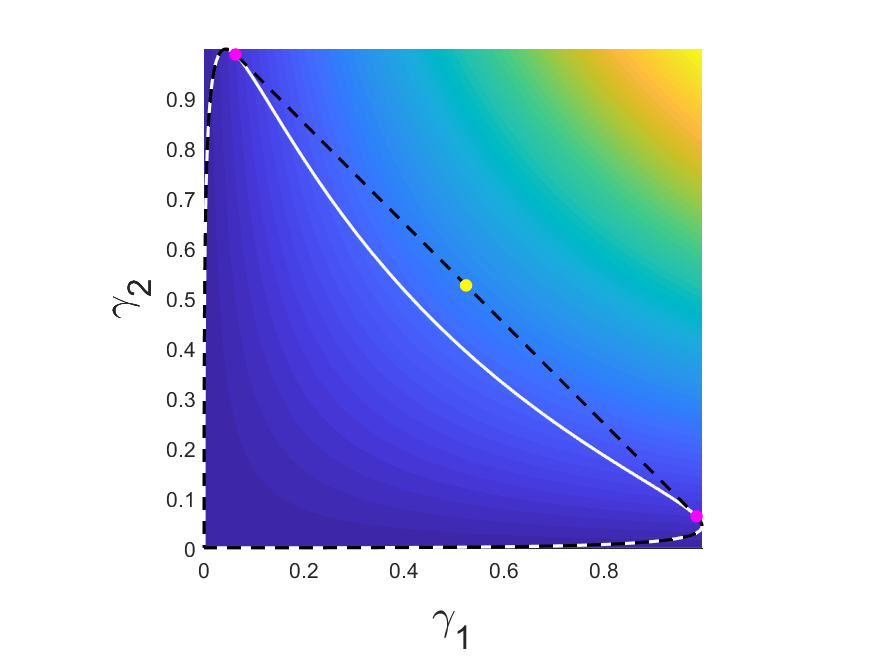
\includegraphics[width = \textwidth]{gamma_likelihood_heatmap}
				\subcaption{}\label{fig:GammaSol:subfig:Gamma}
			\end{minipage}
			\begin{minipage}{0.49\textwidth}
				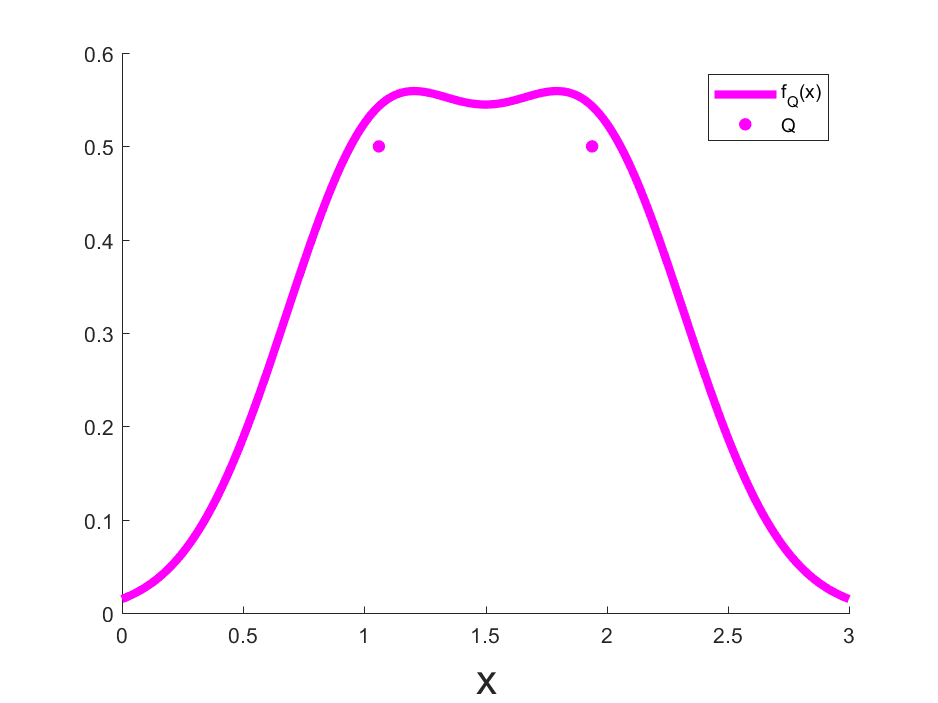
\includegraphics[width = \textwidth]{gamma_likelihood_heatmap_solution}
				\subcaption{}\label{fig:GammaSol:subfig:Density}
			\end{minipage}
			\caption[The geometric relationship between the likelihood curve (\subref{fig:GammaSol:subfig:Gamma}) and the maximizing mixture density (\subref{fig:GammaSol:subfig:Density}).]{The geometric relationship between the likelihood curve (\subref{fig:GammaSol:subfig:Gamma}) and the maximizing mixture density (\subref{fig:GammaSol:subfig:Density}). In (\subref{fig:GammaSol:subfig:Gamma}), the boundary of $\conv(\Gamma_{\vect{x}, f})$ is shown as a dashed black line, $\Gamma_{\vect{x}, f}$ is the white curve, the heat map  shows the objective function (likelihood increases from blue to yellow) and $\hat{\vect{\gamma}}$ is marked with a yellow dot. This point is a convex combination of the two magenta points. These two magenta points correspond to the two probability masses in the maximizing mixing distribution (\subref{fig:GammaSol:subfig:Density}).}
			\label{fig:GammaSol}
		\end{figure}

		\begin{remark}
			Note that in this example, while $\Gamma_{\vect{x}, f}$ is bounded, it is not closed (it does not contain the limit point $(0,0)$), counter to the requirements of Theorems \ref{thm: lindsay maximizing likelihood vector point} and \ref{thm: lindsay no more than n points}. In fact, any positive density whose support is the whole real line will not contain the limit point $\vect{0}$ (where $\vect{0}$ represents the zero vector in $\mathbb{R}^n$). However, since $\vect{0}$ is clearly not going to be a part of a maximizing mixture, we are safe to apply both theorems if $\Gamma \cup \{ \vect{0} \}$ is closed. A more detailed discussion concerning how to relax the requirement that the set $\Gamma_{\vect{x},f}$ be closed can be found in \cite[Section 5.2.2.]{Lindsay1995-sq}.
		\end{remark}

	\subsection{Gradient characterization}
	\label{sec: gradient characterization}
	Another important construction due to Lindsay is the gradient function,
	\begin{equation}
		D_Q(\vect{\theta}; \vect{x}, f) = -n + \sum_{i = 1}^n \frac{f(x_i;\vect{\theta})}{f_Q(x_i)}.
		\label{eq:def gradient function}
	\end{equation}
	For each value of $\theta \in \Omega$, this is the derivative of $l(Q;\vect{x},f)$ as we move along the path parametrized by
	\begin{equation}
		(1 - p)Q + p\Delta_\vect{\theta},
	\end{equation}
	evaluated at $p = 0$ and where $\Delta_\vect{\theta}$ is a degenerate distribution that places all of its mass at $\vect{\theta}$. In \cite[Theorem 4.1]{Lindsay1983-tf}, Lindsay showed that we can use the gradient function to characterise the maximizing mixture using three equivalent conditions. The statement of the Theorem here is taken from \cite[Theorem 19]{Lindsay1995-sq}.

	\begin{theorem}[\cite{Lindsay1995-sq}]
	\label{thm:Lindsay three statements that characterise maximizing mixture}
		The following three statements are equivalent:
		\begin{enumerate}
			\item $\hat{Q}$ maximizes $l(Q;\vect{x},f)$.
			\item $\hat{Q}$ minimizes $\sup_\vect{\theta} D_Q(\vect{\theta};\vect{x}, f)$.
			\item $\sup_\vect{\theta} D_{\hat{Q}}(\vect{\theta};\vect{x}, f) = 0$.
			\label{item:supremum of gradient is zero}
		\end{enumerate}
	\end{theorem}

	The intuition here is that $D_Q(\vect{\theta}; \vect{x}, f)$ measures the change in likelihood as we move a little bit of mass from each of the points of support of $Q$ to a point at $\vect{\theta}$. If a mixing distribution $\hat{Q}$ maximizes the likelihood, then this change in likelihood should never be positive and if we are not at the maximizing distribution $\hat{Q}$, then there should be some $\vect{\theta}$ to which we can move some mass to increase the likelihood.

	% [BLAHBLAH]

	Also contained in \cite[Theorem 4.1]{Lindsay1983-tf} was the following result concerning the locations of the support points of $\hat{Q}$. The statement here is taken from \cite[Theorem 20]{Lindsay1995-sq}.

	\begin{theorem}[\cite{Lindsay1995-sq}]
		\label{thm: Lindsay support is zeros of gradient}
		The support of any maximum likelihood estimator $\hat{Q}$ lies in the set 
		\begin{equation}
			\left\{\vect{\theta} : D_{\hat{Q}}(\vect{\theta};\vect{x},f) = 0 \right\}.
			\label{eq:set D_Q = 0}
		\end{equation}
	\end{theorem}

	Theorems \ref{thm:Lindsay three statements that characterise maximizing mixture} and \ref{thm: Lindsay support is zeros of gradient} indicate that each support point of $\hat{Q}$ is a local maximum of $D_{\hat{Q}}(\vect{\theta}; \vect{x}, f)$. So if $f$ is parametrized by a single parameter $\theta$ and $D_Q(\theta;\vect{x},f)$ is twice differentiable in $\theta$, then each support point $\theta^*$ of the maximizing mixture distribution, $\hat{Q}$, satisfies
	\begin{align}
		D_{\hat{Q}}(\theta^*;\vect{x}, f) &= 0, 
		\label{eq:Deq1}\\
		D'_{\hat{Q}}(\theta^*;\vect{x}, f) &= 0, 
		\label{eq:Deq2}\\
		D''_{\hat{Q}}(\theta^*;\vect{x}, f) &\leq 0,
		\label{eq:Deq3}
	\end{align}
	so long as $\theta^*$ is not on the boundary of the parameter space. A typical example of this is shown in Figure \ref{fig:D_Q example}. In this figure we observe that $D_Q(\theta)$ has a local maximum at every point where $Q$ places a probability mass. Since $D_Q(\theta) \leq 0$ for all $\theta \in \mathbb{R}$, we know that $Q$ is the maximum likelihood mixing distribution. In Section \ref{sec:KKT conditions} we will show how to obtain equations \eqref{eq:Deq1} and \eqref{eq:Deq2} using a different method to Lindsay that does not involve the gradient function.

	% [EXAMPLE]

	\begin{figure}[ht]
		\begin{subfigure}[t]{0.49\textwidth}
			\centering
			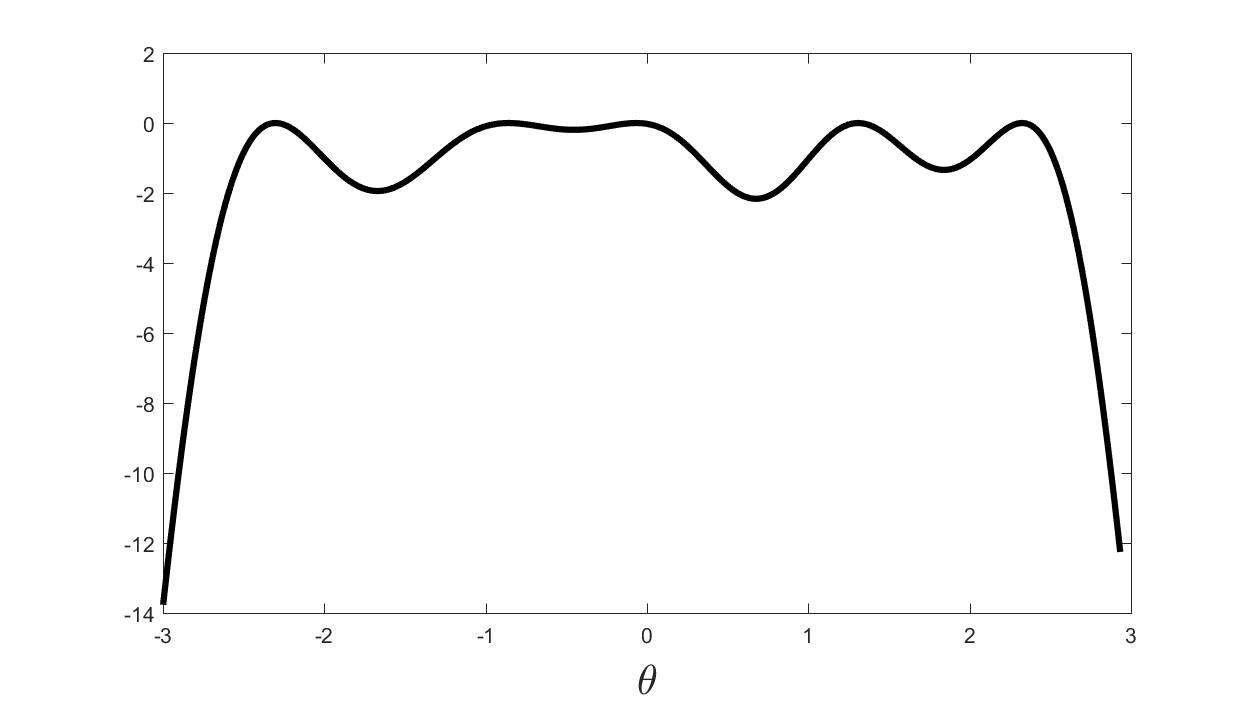
\includegraphics[width = \textwidth]{Figures/Mixtures/D_Q_example.png}
			\caption{}\label{subfig:D_Q}
		\end{subfigure}
		\begin{subfigure}[t]{0.49\textwidth}
			\centering
			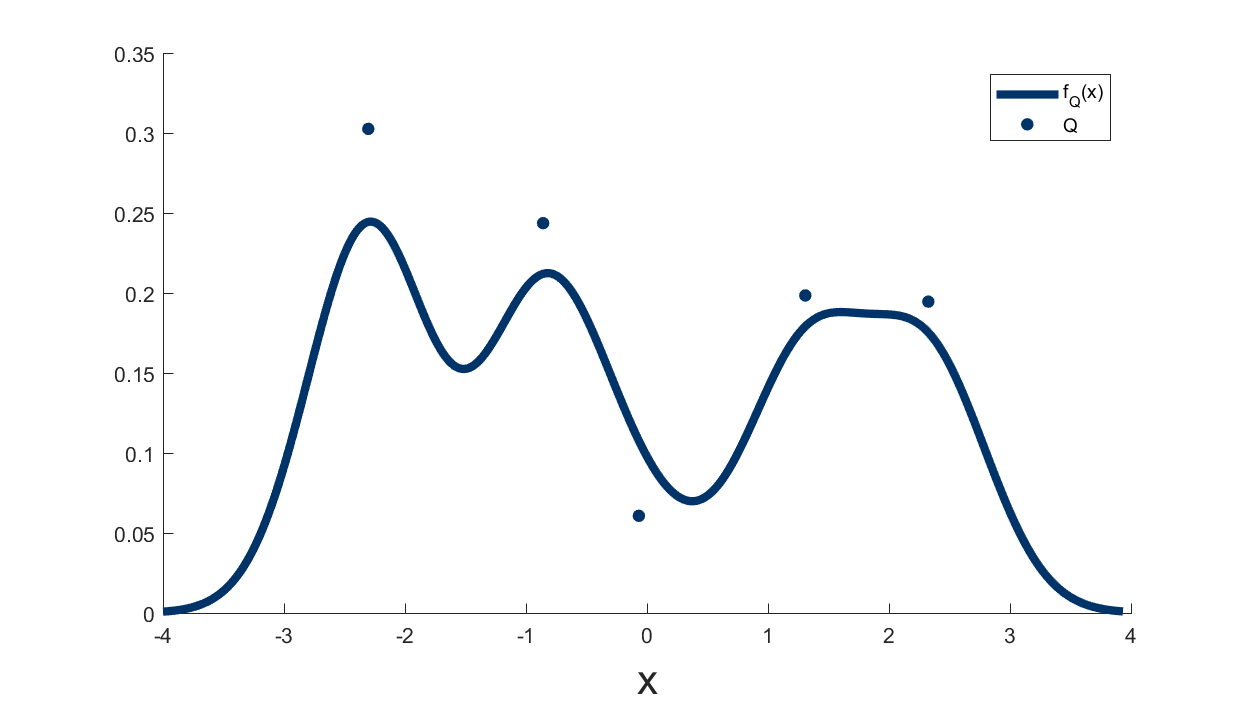
\includegraphics[width = \textwidth]{Figures/Mixtures/D_Q_example_mixture.png}
			\caption{}\label{subfig:D_Qmixture}
		\end{subfigure}
		\caption[The gradient function and its associated mixing distribution and mixture.]{The gradient function, $D_{\hat{Q}}$, (\subref{subfig:D_Q}) and its associated mixing distribution, $Q$, and mixture, $f_Q$, (\subref{subfig:D_Qmixture}). In this example $f$ is normal with variance $1/4$ and $\vect{x}$ is made up of $n = 50$ points distributed uniformly but randomly along $[-3, 3]$.}
		\label{fig:D_Q example}
	\end{figure}

	\subsubsection{Support Hyperplane}
	\label{sec: support hyperplane}
	There is a geometric interpretation to these theorems that ties in with the likelihood curve interpretation given above. For any given mixing distribution $Q$, define the \emph{inverse likelihood vector} $\vect{\lambda}(Q;\vect{x},f) = (1/f_Q(x_1),\dots, 1/f_Q(x_n))$ and the hyperplane
	\begin{equation}
		\mathcal{H}_{Q} = \{\vect{z} : \langle \vect{\lambda}(Q;\vect{x},f), \vect{z}\rangle = n\},
	\end{equation}
	which contains the usual likelihood vector, $\vect{\gamma}(Q;\vect{x}, f)$. We may write the gradient function as
	\begin{equation}
		D(Q;\vect{x},f) = \langle \vect{\lambda}(Q;\vect{x},f), \vect{\gamma}(\vect{\theta};\vect{x},f)\rangle - n.
	\end{equation}
	If $\hat{Q}$ maximizes $l(Q;\vect{x},f)$ then by statement \ref{item:supremum of gradient is zero} of Theorem \ref{thm:Lindsay three statements that characterise maximizing mixture}, 
	\begin{equation}
		\langle \vect{\lambda}(\hat{Q};\vect{x},f), \vect{\gamma}(\vect{\theta};\vect{x},f) \rangle \leq n
	\end{equation}
	for all $\vect{\theta} \in \Omega$. This means that $\mathcal{M} = \conv(\Gamma_{\vect{x},f})$ lies entirely on one side of $\mathcal{H}$ and Theorem \ref{thm: Lindsay support is zeros of gradient} tell us that if $\vect{\theta}$ is in the support of $\hat{Q}$, then 
	\begin{equation}
		\langle \vect{\lambda}(\hat{Q};\vect{x},f), \vect{\gamma}(\vect{\theta};\vect{x},f) \rangle = n
	\end{equation}
	and so $\vect{\gamma}(\vect{\theta};\vect{x},f) \in \mathcal{H}$. Thus we can gain information about the number of support points of $\hat{Q}$ by finding the number of points at which $\Gamma_{\vect{x},f}$ touches $\mathcal{H}_{\hat{Q}}$. As an example, consider Figure \ref{fig:cauchy support hyperplane}. Here we observe the likelihood curve for a Cauchy density and $n = 2$ observations. The support line containing $\hat{\vect{\gamma}}$ has two points of contact with $\Gamma_{\vect{x}, f}$ which correspond to the two points of support of the maximum likelihood mixture $\hat{Q}$. In our experience it is fairly typical for every contact point of $\Gamma_{\vect{x}, f}$ with $\mathcal{H}_{\hat{Q}}$ (or equivalently, every point in \eqref{eq:set D_Q = 0}) to correspond to a support point of $\hat{Q}$. However, this is not always the case. In Figure \ref{fig:triangle support hyperplane} we have shown the likelihood curve for a symmetric triangular density and $n =2$ observations. We observe that $\mathcal{H}_{\hat{Q}}$ touches $\Gamma_{\vect{x}, f}$ at an infinite number of points along a line segment. The interpretation is that there are an infinite number of distinct mixtures which achieve the maximum likelihood, each with support points corresponding to various locations along that line segment.

	\begin{figure}
		\centering
		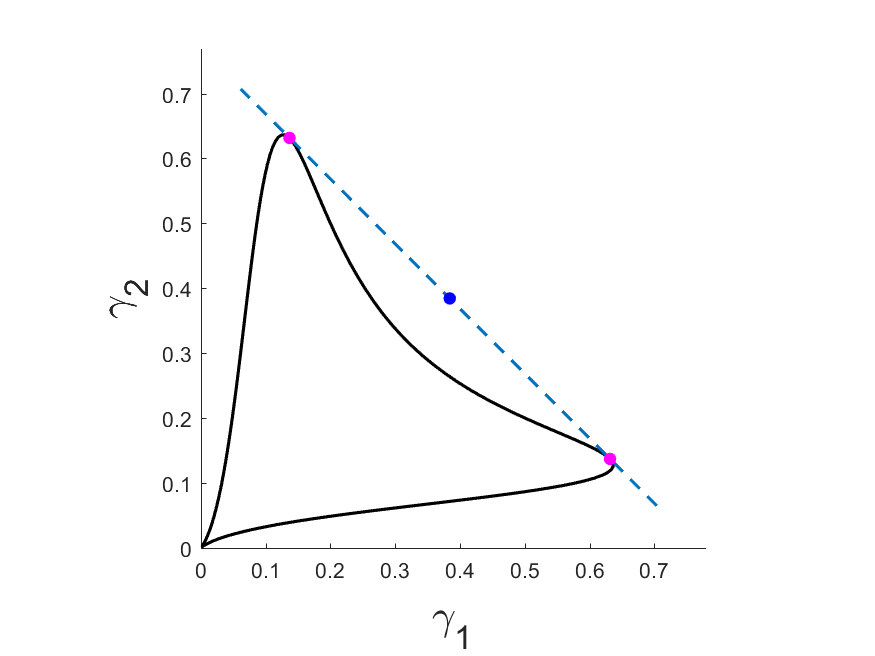
\includegraphics[width = 0.9\textwidth]{Figures/Mixtures/cauchy_support_hyperplane.png}
		\caption{The likelihood curve, $\Gamma_{\vect{x}, f}$, (solid line) along with the support hyperplane, $\mathcal{H}_{\hat{Q}}$, (dashed line) that contains $\hat{\vect{\gamma}}$ (blue point), and the points of contact with $\Gamma_{\vect{x}, f}$ (magenta points). In this example $\vect{x} = (1,2)$ and $f$ is a Cauchy density with scale parameter $1/2$.}
		\label{fig:cauchy support hyperplane}
	\end{figure}

	\begin{figure}
		\centering
		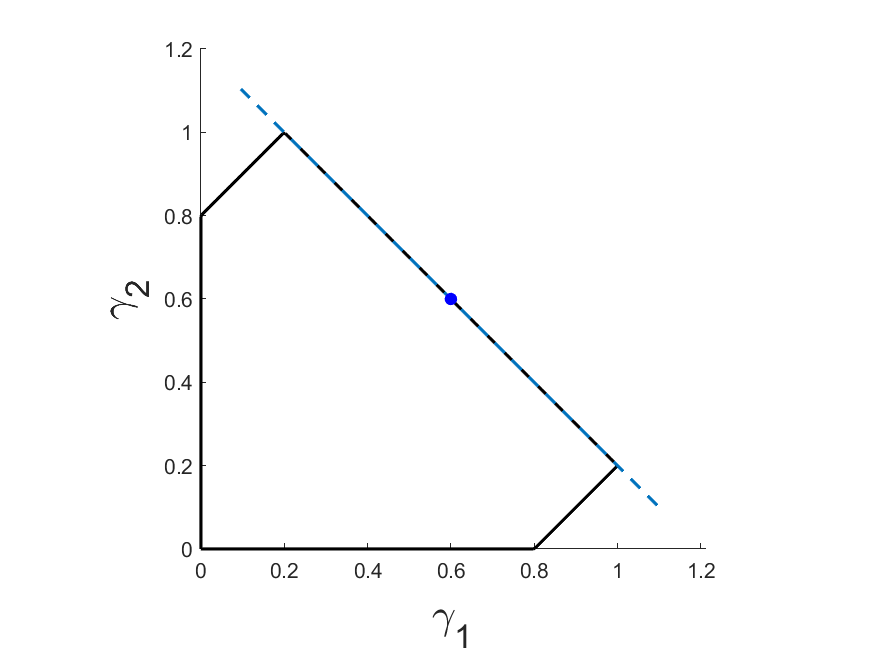
\includegraphics[width = 0.9\textwidth]{Figures/Mixtures/triangle_density_gamma.png}
		\caption{The likelihood curve, $\Gamma_{\vect{x}, f}$, (solid line) along with the support hyperplane, $\mathcal{H}_{\hat{Q}}$, (dashed line) that contains $\hat{\vect{\gamma}}$ (blue point). In this example $\vect{x} = (0,0.4)$ and $f$ is a symmetric triangular density with width $1/2$.}
		\label{fig:triangle support hyperplane}
	\end{figure}

	\subsection{KKT conditions}
	\label{sec:KKT conditions}
	We will now point out that the gradient function conditions in \eqref{eq:Deq1} and \eqref{eq:Deq2} can be obtained using the Karush-Kuhn-Tucker (KKT) conditions \cite{Kuhn1951-ih} \cite{Karush2014-vk} for the following optimisation problem. Suppose that we restrict our mixture to have no more than $m$ components. Then given a component density $f$, and data $\vect{x}$, %the problem of finding the maximum likelihood location mixture can be written as the following non-linear optimization problem.
%
	find $\vect{\theta}$ and $\vect{p}$ that maximize
	\begin{equation}
		l_m(\vect{\theta},\vect{p};\vect{x}) = \sum_{i=1}^n \log \left[\sum_{j=1}^m p_j f(x_i - \theta_j) \right]
		\label{eq:l_m}
	\end{equation}
	subject to 
	\begin{align}
		&\theta_j -\theta_{j+1} \leq 0, &&j=1,\dots,m-1
		\label{eq:constraintheta}\\
		&-p_j \leq 0, &&j=1,\dots,m
		\label{eq:constrainpj}\\
		&\sum_{j=1}^m p_j = 1.
		\label{eq:constrainpjequal}
	\end{align}

	Constraints \eqref{eq:constrainpj} and \eqref{eq:constrainpjequal} ensure that the mixture is valid. We also include \eqref{eq:constraintheta} so that any mixture which can be written with fewer than $m$ components appears on the boundary of the feasible space (we will either have some $p_j = 0$ or some $\theta_j = \theta_{j+1}$). Conversely, any point at which we have equality in any of the constraints in \eqref{eq:constraintheta} or \eqref{eq:constrainpj}, can be written with fewer than $m$ components. Hence, a necessary condition for $K_\vect{x} = m$ is that any maximizing point of \eqref{eq:l_m} must also satisfy strict inequalities in \eqref{eq:constraintheta} and \eqref{eq:constrainpj}.

	Introduce Lagrange multipliers $\lambda$, $\vect{\mu}$, $\vect{\nu}$ and form the Lagrangian
	\begin{equation}
		\mathcal{L}(\vect{\theta},\vect{p},\lambda,\vect{\mu},\vect{\nu}) = l_m(\vect{\theta},\vect{p};\vect{x}) - \lambda\left(1 - \sum_{j=1}^m p_j\right) - \sum_{j=1}^m \mu_j p_j + \sum_{j=1}^{m-1} \nu_j \left(\theta_j - \theta_{j+1}\right).
		\label{eq:kkt lagrangian}
	\end{equation}
	The KKT conditions tell us that at a local maximum the equations
	\begin{align}
		&\frac{\partial}{\partial \theta_1} l_m(\vect{\theta},\vect{p};\vect{x}) = \nu_1, \label{eq:KKTtheta1}\\ 
		&\frac{\partial}{\partial \theta_j} l_m(\vect{\theta},\vect{p};\vect{x}) = \nu_j - \nu_{j-1}, &&j=2,\dots,m-1 \label{eq:KKTtheta},\\ 
		&\frac{\partial}{\partial \theta_m} l_m(\vect{\theta},\vect{p};\vect{x}) = -\nu_{m-1} \label{eq:KKTthetam},\\ 
		&\frac{\partial}{\partial p_j} l_m(\vect{\theta},\vect{p};\vect{x}) = \lambda - \mu_j, && j = 1,\dots,m, \label{eq:KKTlambda}
	\end{align}
	must be satisfied along with the constraints in \eqref{eq:constraintheta}, \eqref{eq:constrainpj}, \eqref{eq:constrainpjequal}, and the additional constraints
	\begin{align}
		&\vect{\mu},\vect{\nu} \geq 0,\\
		&\mu_j p_j = 0, &&j=1,\dots,m, \label{eq:mujpjconstraint}\\
		&\nu_j (\theta_j - \theta_{j+1}) = 0, &&j=1,\dots,m-1.
		\label{eq:nujthetajconstraint}
	\end{align}

	Multiplying both sides of \eqref{eq:KKTlambda} by $p_j$ (recall \eqref{eq:mujpjconstraint}) and summing over $j$ we get that
	\begin{equation}
		\lambda = \sum_{j = 1}^m p_j \frac{\partial}{\partial p_j} l_m(\vect{\theta},\vect{p};\vect{x}).
	\end{equation}
	From \eqref{eq:l_m},
	\begin{align}
		\lambda &= \sum_{j = 1}^m p_j \frac{\partial}{\partial p_j} \left( \sum_{i=1}^n \log \left[\sum_{k=1}^m p_k f(x_i - \theta_k) \right] \right)\\
			&= \sum_{j = 1}^m p_j \sum_{i=1}^n \frac{f(x_i - \theta_j)}{\sum_{k=1}^m p_k f(x_i - \theta_k)}\\
			&= \sum_{i=1}^n \sum_{j=1}^m  \frac{p_j f(x_i - \theta_j)}{\sum_{k=1}^m p_k f(x_i - \theta_k)}\\
			&= n.
	\end{align}

	If we additionally require that the solution uses all $m$ components, then we must have that $p_j > 0$, and $\theta_j - \theta_{j+1} < 0$ for all $j$. Constraints \eqref{eq:mujpjconstraint} and \eqref{eq:nujthetajconstraint} then require $\mu_j = 0$ and $\nu_j = 0$ for all $j$. This gives us necessary conditions for $\hat{Q} = (\vect{\theta}, \vect{p})$ to be an $m$ point maximizing mixture,
	\begin{align}
		&-n + \frac{\partial}{\partial p_j} l_m(\vect{\theta},\vect{p};\vect{x}) = 0, && j = 1,\dots,m,\\
		&\frac{\partial}{\partial \theta_j} l_m(\vect{\theta},\vect{p};\vect{x}) = 0, && j = 1,\dots, m.
	\end{align}
	Substituting in $l_m$ from \eqref{eq:l_m} we obtain
	\begin{align}
		&-n + \sum_{i=1}^n \frac{f(x_i - \theta_j)}{f_{\hat{Q}}(x_i)} = D_{\hat{Q}}(\theta_j;\vect{x}, f) =  0, && j = 1, \dots, m, \label{eq:KKT Deq1}\\
		&\sum_{i=1}^n \frac{-p_jf'(x_i - \theta_j)}{f_{\hat{Q}}(x_i)} = p_j D_{\hat{Q}}'(\theta_j;\vect{x}, f) = 0, && j = 1, \dots, m,
		\label{eq:KKT Deq2}
	\end{align}
	which are equivalent to \eqref{eq:Deq1} and \eqref{eq:Deq2} respectively.

	% [KEEP THIS SECOND ORDER STUFF IN?]
	% [COMMENT ON LINDSAY THM 7.1]
	% [CHECK FOR MISTAKES IN MY WORK AND LINDSAY'S]
	% [IF NO MISTAKES SAY "NOT WHAT WE GOT" (if they are comparable)]

	The second order conditions are slightly more complex. In the context of our problem they state \cite[Proposition 3.3.1]{Bertsekas1995-mh} that a necessary condition for the point $(\vect{\theta}, \vect{p}, \lambda, \vect{\mu}, \vect{\nu})$ to be a local maximum is that,
	% \begin{equation}
	% 	y' 
	% 	\begin{bmatrix}
	% 		\frac{\partial^2}{\partial \theta_1^2} & \frac{\partial^2}{\partial \theta_1 \theta_2} & \dots & \frac{\partial^2}{\partial \theta_1 p_1} & \dots\\
	% 		\frac{\partial^2}{\partial \theta_2 \theta_1} & \frac{\partial^2}{\partial \theta_1^2} & \dots & \vdots  & \dots\\
	% 		\vdots & & \ddots & &\\
	% 		\vdots & & & \frac{\partial^2}{\partial p_1^2} &\\
	% 		\vdots & & \ddots & &
	% 	\end{bmatrix} y \geq 0.
	% \end{equation}
	\begin{equation}
		\vect{y}' \nabla^2_{\vect{\theta}, \vect{p}} \mathcal{L}(\vect{\theta}, \vect{p}, \lambda, \vect{\mu}, \vect{\nu}) \vect{y} \leq 0
		\label{eq:KKT second order}
	\end{equation}
	for all $\vect{y} \in \mathbb{R}^{2m}$ such that
	\begin{equation}
		\nabla h(\vect{\theta}, \vect{p})' \vect{y} = 0,
	\end{equation}
	where
	\begin{equation}
		h(\vect{\theta}, \vect{p}) = 1 - \sum_{j = 1}^m p_j.
	\end{equation}
	Since 
	\begin{equation}
		\nabla h(\vect{\theta}, \vect{p}) = (0, \dots, 0, -1, \dots, -1),
	\end{equation}
	equation \eqref{eq:KKT second order} must be satisfied in particular for $\vect{y}$ with components $y_k = 1$ for some $k \leq m$ and $y_i  = 0$ for all $i \neq k$. This gives us that necessary conditions for $\hat{Q}$ to be an $m$ point maximum are that
	\begin{align}
		\frac{\partial^2}{\partial \theta_j} \mathcal{L}(\vect{\theta}, \vect{p}, \lambda, \vect{\mu}, \vect{\nu}) &\leq 0, && j = 1, \dots, m.
	\end{align}
	Recalling \eqref{eq:kkt lagrangian} and \eqref{eq:l_m}, we get that
	\begin{align}
		\frac{\partial^2}{\partial \theta_j} \mathcal{L}(\vect{\theta}, \vect{p}, \lambda, \vect{\mu}, \vect{\nu}) &= \sum_{i = 1}^n \frac{p_j f''(x_i - \theta_j)}{\sum_{k = 1}^m p_k f(x_i - \theta_k)} - \sum_{i = 1}^n \left(\frac{p_j f'(x_i - \theta_j)}{\sum_{k = 1}^m p_k f(x_i - \theta_k)}\right)^2 \\
		&= p_j D_Q''(\theta_j;\vect{x}, f) - \sum_{i = 1}^n \left(\frac{p_j f'(x_i - \theta_j)}{\sum_{k = 1}^m p_k f(x_i - \theta_k)}\right)^2 \\
		&\leq 0.
	\end{align}
	Overall, we have that at every support point, $\theta^*$, of an $m$-point maximizing mixture, $Q$, we must have that
	\begin{equation}
		D_Q''(\theta^*;\vect{x},f) \leq p^* \sum_{i = 1}^n \left(\frac{f'(x_i - \theta_j)}{\sum_{k = 1}^m p_k f(x_i - \theta_k)}\right)^2.
		\label{eq: our second order KKT condition}
	\end{equation}
	This is a weaker condition than that in \eqref{eq:Deq3}. We were unable to obtain an equivalent condition to \eqref{eq:Deq3} using the above method. This is somewhat expected as we have restricted our mixture to have no more than $m$ components, whereas the condition in \eqref{eq:Deq3} relates to the global maximizing mixture distribution.

	We note that Lindsay presented a similar result in \cite[Theorem 7.1]{Lindsay1983-tf} and \cite[Theorem 24]{Lindsay1995-sq} which concerned maximum likelihood estimators with a fixed number of components. Below we rewrite this statement in the context of location mixtures.
	\begin{claim}[\cite{Lindsay1995-sq}, Theorem 24]
	\label{thm:Lindsay m-point conditions}
		Let $\tilde{Q}_m$ be a mixing distribution that maximizes the $m$ component location mixture likelihood, and let $\theta^*$ be a support point of $\tilde{Q}_m$. If the gradient function is twice differentiable at $\theta^*$, then:
		\begin{align}
			D_{\tilde{Q}_m}(\theta^*; \vect{x}, f) &= 0,\\
			D_{\tilde{Q}_m}'(\theta^*; \vect{x}, f) &= 0,\\
			D_{\tilde{Q}_m}''(\theta^*; \vect{x}, f) &\leq \sum_{i = 1}^n \left(\frac{f(x_i - \theta^*)}{\sum_{k = 1}^m p_k f(x_i - \theta_k)}\right)^2.
			\label{eq:Lindsay m-point Deq 3}
		\end{align}
	\end{claim}

	Equations \eqref{eq: our second order KKT condition} and \eqref{eq:Lindsay m-point Deq 3} appear similar in form but are not equivalent. Lindsay did not provide a proof for his statement but asserted that Claim \ref{thm:Lindsay m-point conditions} can be proved in a straightforward way using the likelihood equations and the formula for the gradient. We are unable to replicate his result, and instead present a counter-example to Claim \ref{thm:Lindsay m-point conditions}.

	Let our component density $f$ be normal with unit variance, and let $\vect{x} = (-2,2)$. Consider the mixing distribution, $\tilde{Q}_1$, that maximizes the 1 component location mixture likelihood. It has one support point, $\theta_1$. The gradient function for this distribution is given by
	\begin{equation}
		D_{\tilde{Q}_1}(\theta;\vect{x}, f) = -n + \sum_{i = 1}^2 \frac{f(x_i - \theta)}{f(x_i - \theta_1)},
	\end{equation}
	with derivatives
	\begin{equation}
		D_{\tilde{Q}_1}'(\theta;\vect{x}, f) = \sum_{i = 1}^2 \frac{-f'(x_i - \theta)}{f(x_i - \theta_1)} = \sum_{i = 1}^2 \frac{(x_i - \theta) f(x_i - \theta)}{f(x_i - \theta_1)}
	\end{equation}
	and
	\begin{equation}
		D_{\tilde{Q}_1}''(\theta;\vect{x}, f) = \sum_{i = 1}^2 \frac{f''(x_i - \theta)}{f(x_i - \theta_1)} = \sum_{i = 1}^2 \frac{((x_i - \theta)^2 - 1)f(x_i - \theta)}{f(x_i - \theta_1)},
	\end{equation}
	where
	\begin{equation}
		f(x) = \frac{1}{\sqrt{2 \pi}} \exp\left(-\frac{x^2}{2}\right).
	\end{equation}
	By \eqref{eq:KKT Deq2}, we must have that $D'_{\tilde{Q}_1}(\theta_1;\vect{x}, f) = (x_1 - \theta_1) + (x_2 - \theta_1) = 0$ and so $\theta_1 = 0$. Then it is simple to calculate
	\begin{equation}
		D_{\tilde{Q}_1}''(\theta_1;\vect{x}, f) = 6
	\end{equation}
	and
	\begin{equation}
		\sum_{i = 1}^n \left(\frac{f(x_i - \theta_1)}{\sum_{k = 1}^m p_k f(x_i - \theta_k)}\right)^2 = 2.
	\end{equation}
	Clearly \eqref{eq:Lindsay m-point Deq 3} does not hold. 

	By way of comparison, 
	\begin{equation}
		p_1 \sum_{i = 1}^n \left(\frac{f'(x_i - \theta_1)}{\sum_{k = 1}^m p_k f(x_i - \theta_k)}\right)^2 = \sum_{i = 1}^2 x_i^2 = 8,
	\end{equation}
	verifying that \eqref{eq: our second order KKT condition} holds for this example.


	\subsection{Additional results on \texorpdfstring{$K_\vect{x}$}{Kx}}

	Theorem \ref{thm: lindsay no more than n points} bounds $K_\vect{x}$ by $n$. To get tighter bounds on $K_\vect{x}$, we must make some assumptions about the form of the component densities, or the structure of $\vect{x}$.

	In \cite{Lindsay1983a-he}, Lindsay looked at the special case of  component densities in the exponential family. He related the behaviour of certain polynomials to the location of the support points of the maximizing mixture. A consequence of this was a sufficient condition for the maximizing mixture to have exactly one point of support. We restate part of this theorem here.

	\begin{theorem}[Theorem 4.1, \cite{Lindsay1983a-he}]
	\label{thm:exponential family k=1 bound}
		Let $f_\theta$ belong to the exponential class of densities and be parametrized by its mean value $\theta$. Let $\vect{x} = (x_1, \dots, x_n)$, $x_1 \leq \dots \leq x_n$, be the sample for which we are finding the maximum likelihood mixture of $f_\theta$. Define the function
		\begin{equation}
			M(\theta) = (x_1 - \theta)(x_n - \theta) + \var_\theta(X).
		\end{equation}
		If $M(\theta)$ is strictly positive on $[x_1, x_n]$, then the maximimum likelihood mixing distribution, $\hat{Q}$, has exactly one point of support located at $\theta = \bar{x}$.
	\end{theorem}

	The above is a sufficient condition for $K_\vect{x} = 1$. However, Linsday also showed that in the case of two observations ($n=2$), one could easily visualise the likelihood curve for a location mixture of normals and observe that the above sufficient condition also seems to be necessary for a normal density. 
	% \subsection{The likelihood curve when \texorpdfstring{$n = 2$}{n = 2}}
		% The shape of $\Gamma_\vect{x}$ can provide us with some insight into the behaviour of $K_\vect{x}$. 

	We illustrate this in Figure \ref{fig:Gammaexample} by giving some examples of $\Gamma_\vect{x}$ for $n=2$ using a normal component density with variance $\sigma^2 = 1$. 
	\begin{figure}[ht]
		\begin{subfigure}[t]{0.32\textwidth}
			\centering
			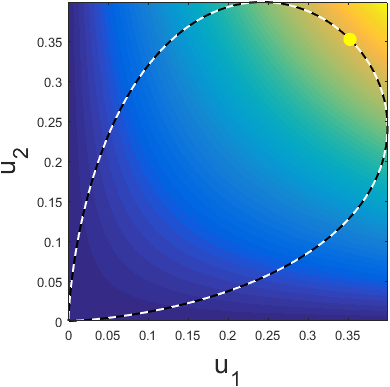
\includegraphics[width = \textwidth]{Sigma1x1_0-x2_1}
			\caption{$\vect{x} = (0,1)$} \label{subfig:gammaexamplea}
		\end{subfigure}
		\begin{subfigure}[t]{0.32\textwidth}
			\centering
			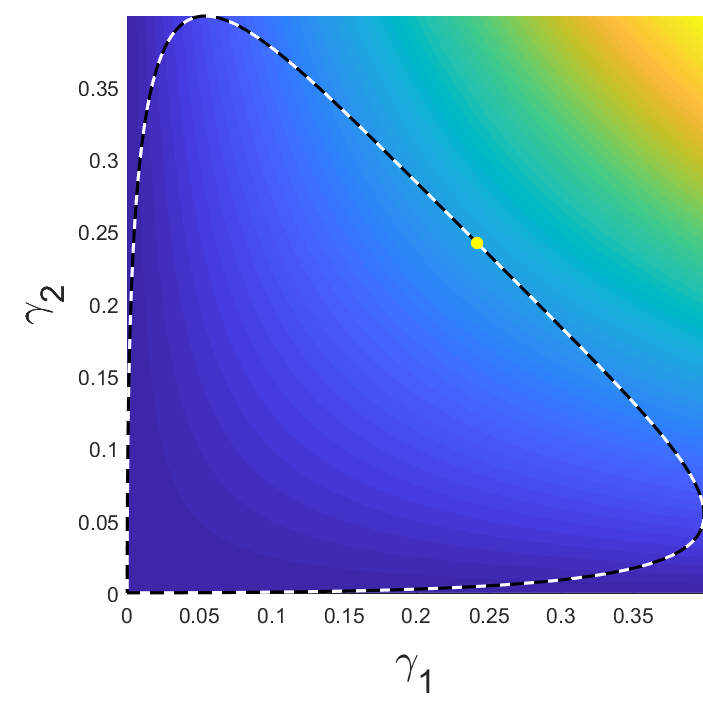
\includegraphics[width = \textwidth]{Sigma1x1_0-x2_2}
			\caption{$\vect{x} = (0,2)$} \label{subfig:gammaexampleb}
		\end{subfigure}
		\begin{subfigure}[t]{0.32\textwidth}
			\centering
			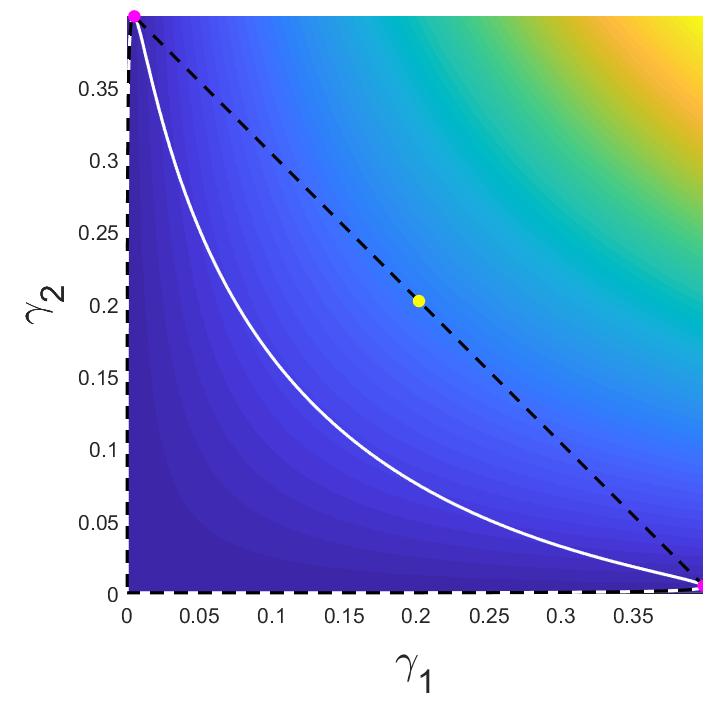
\includegraphics[width = \textwidth]{Sigma1x1_0-x2_3}
			\caption{$\vect{x} = (0,3)$} \label{subfig:gammaexamplec}
		\end{subfigure}
		\caption[The curve $\Gamma_\vect{x}$ for three different $\vect{x}$ along with the boundary of $\conv(\Gamma_\vect{x})$ for a normal component density with unit variance.]{The curve $\Gamma_\vect{x}$ for three different $\vect{x}$ along with the boundary of $\conv(\Gamma_\vect{x})$ for a normal component density with unit variance. The objective function, $\mathcal{L}(\vect{\gamma})$, is represented as a heat map. The optimal point $\hat{\vect{\gamma}}$ is shown in yellow, and where applicable, the points $\vect{\gamma}(\theta_j)$ that make up $\hat{\vect{\gamma}}$ are shown in magenta.}
		\label{fig:Gammaexample}
	\end{figure}
%
	In particular, we note that the distance between $x_1$ and $x_2$ has a strong effect on the shape of $\Gamma_\vect{x}$. In Figure \ref{subfig:gammaexamplea}, the points are distance 1 apart and $\Gamma_\vect{x}$ is the boundary of $\conv(\Gamma_\vect{x})$. In this case, it is clear that $K_\vect{x} = 1$. In Figure \ref{subfig:gammaexamplec}, the points are distance 3 apart and the optimal point no longer lies on $\Gamma_\vect{x}$. This results in the maximum likelihood mixing distribution needing two points of support and so $K_\vect{x} = 2$. The boundary case, where $\Gamma_\vect{x}$ goes from being a convex curve to having the indentation shown in Figure \ref{subfig:gammaexamplec}, is shown in Figure \ref{subfig:gammaexampleb}. This corresponds to the maximum separation the two points can have while keeping $M(\theta)$ non-negative on $[x_1, x_n]$.


	% Obtaining results about where these boundaries lie is very difficult in higher dimensions. In \cite{Lindsay1983a-he}, Lindsay used the sign of the curvature of $\vect{\gamma}(\theta;\vect{x})$ to obtain results for $n=2$ when the component density is in the exponential family.
	Lindsay stated that "these results were very difficult to obtain in higher dimensions, and hard to generalize outside the exponential family" \cite{Lindsay1995-sq}. Some generalizations to the results in \cite{Lindsay1983a-he} were presented in \cite{Lindsay1993-rj}. This paper gave improved bounds on $K_\vect{x}$ for discrete component densities.

	In Section \ref{sec:mixture results} we will present a necessary and sufficient condition for $K_\vect{x} = 1$ in the case of two observations for a certain class of densities that include the normal density, as well as other densities outside the exponential family. We will also present a necessary condition for $K_\vect{x} = m$, $m = 1, \dots, n$, for normal densities in the case of $n$ observations.

	% [WE USE UNIMODALITY TO BE ABLE TO JUST LOOK AT CURVATURE ALONG INTERVAL]

	% [FOLLOWING IS NOTES FOR MYSELF]

	% Exponential family \cite{Lindsay1983a-he}, more general results including this one and others in \cite{Lindsay1993-rj}. In particular, $n/2$ for discrete densities. May want to cite \cite{Seregin2010-xe} since it has some very limited results on the support. Read \cite{Zhang2008-wn} for more citations.
	

	% \subsection{Directional Derivative}
	% 	One of the tools introduced in \cite{Lindsay1983-tf} was the function
	% 	\begin{equation}
	% 		D(\theta;\vect{p},\vect{\theta},\vect{x}) = -n + \sum_{i=1}^n \frac{f(x_i - \theta)}{\sum_{j=1}^m p_j f(x_i - \theta_j)}.
	% 	\end{equation}

	% 	Lindsay showed that if $\hat{\vect{\theta}}$ and $\hat{\vect{p}}$ form a maximum likelihood location mixture of $f$ for $\vect{x}$ then (under appropriate differentiability assumuptions) the function $D$ satisfies the following:
	% 	% \begin{align}
	% 	% 	D(\theta_k;\hat{\vect{p}},\hat{\vect{\theta}},\vect{x}) &= 0, && k = 1,\dots,m,
	% 	% 	\label{eq:Deq1}\\
	% 	% 	D'(\theta_k;\hat{\vect{p}},\hat{\vect{\theta}},\vect{x}) &= 0, && k = 1,\dots,m,
	% 	% 	\label{eq:Deq2}\\
	% 	% 	D''(\theta_k;\hat{\vect{p}},\hat{\vect{\theta}},\vect{x}) &\leq 0, && k = 1,\dots,m.
	% 	% 	\label{eq:Deq3}
	% 	% \end{align}
	% 	These three constraints restrict what a potential maximum likelihood solution can look like.
	% 	HOW DID LINDSAY USE THEM VS US?


\section{Empirical Results}
\label{sec:empirical results}
	In this section we explore $K_\vect{x}$ through empirical results and figures. Throughout this section, and for the remainder of this chapter, we will consider only location mixtures (see \eqref{eq:location mixture}). All component densities will be unimodal, with a mode at $x = 0$. We list in Table \ref{tab:component densities} the component densities that we will use.

	\begin{table}[ht]
	\centering
		\begin{tabular}{l | c}
			Density & $f(x) = $\\
			\hline
			normal with fixed variance $\sigma^2$ & $\frac{1}{\sigma \sqrt{2 \pi}} \exp\left(-\frac{x^2}{2\sigma^2}\right) $\\
			Cauchy with fixed scale $\gamma$ & $\frac{1}{\pi \gamma + \pi x^2/\gamma}$
		\end{tabular}	
		\caption{List of component densities we consider.}
		\label{tab:component densities}
	\end{table}
	

	\subsection{Method}
	There are two parts to determining $K_\vect{x}$ empirically. The first part is to find the maximum likelihood mixture, $\hat{Q}$, or at least a good approximation $Q^*$. Given $\vect{x} \in \mathbb{R}^n$, we use a general purpose nonlinear programming solver (the MATLAB function \emph{fmincon}) to find the maximum likelihood mixture. We can test that we have indeed reached the global maximum through the use of the derivative function conditions given in Theorem \ref{thm:Lindsay three statements that characterise maximizing mixture}. If the mixture that is returned by our general solver does not satisfy these conditions then we may use another method, such as the vertex direction method (VDM) or the vertex exchange method (VEM), which is guaranteed to converge to the global maximum but converges slowly (see \cite{Bohning1995-di} for a review of different methods). We note that the actual method used is not important so long as the final result satisfies the derivative conditions. In practice, when $n$ is small, a general purpose solver is sufficient, fast, and simple to implement, and we rarely need to use a secondary method.

	The second part is to determine the number of points of support of $Q^*$. We initiate our general purpose solver with a mixture distribution that has more points of support than is needed. Under the optimization, this collapses down to the distribution $Q^*$ which may assign zero weight to some masses, and may concentrate multiple masses on the one point of support. We may simplify such a distribution by removing all masses with zero weight, and by combining all masses which share a point of support into one mass which takes the combined weight of the constituent masses (see Figure \ref{fig:collapsing distribution}). A naive approach would be to take the number of probability masses in this simplified distribution as the value for $K_\vect{x}$.

	\begin{figure}
		\centering
		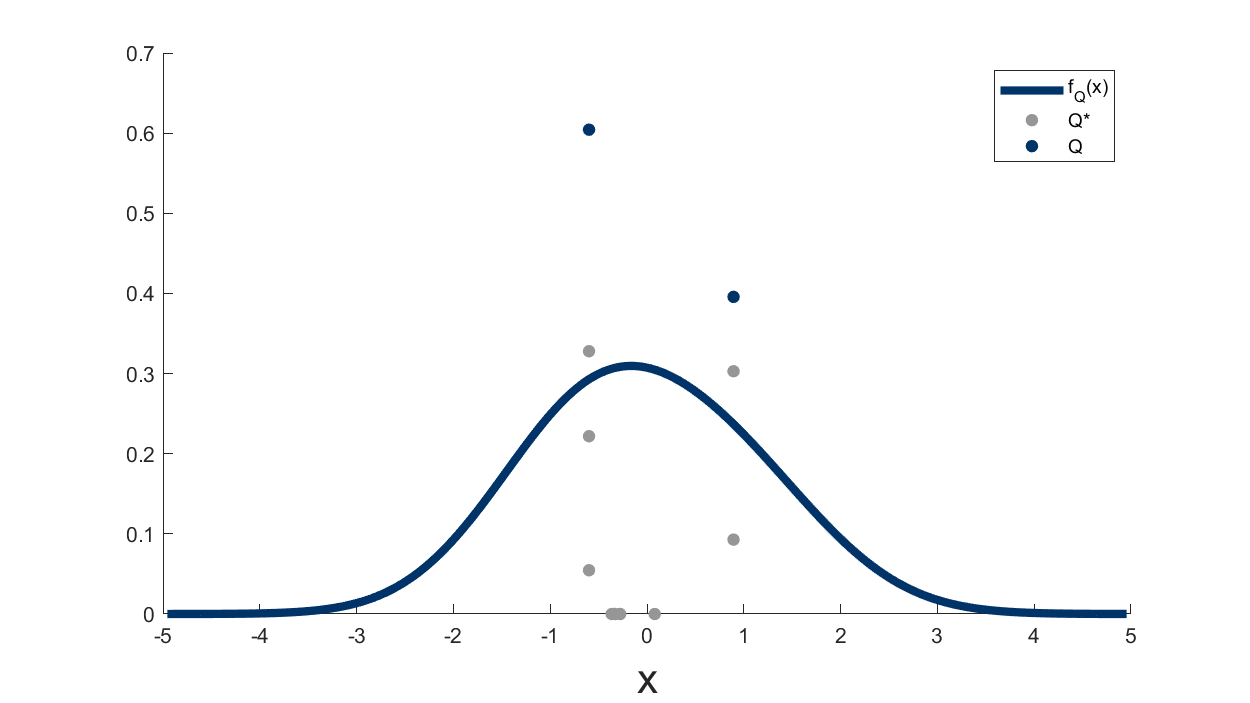
\includegraphics[width = \textwidth]{Figures/Mixtures/collapsing_distribution.png}
		\caption[The unsimplified mixing distribution $Q^*$ that results from using more points of support than required when finding our maximizing mixture, as well as the equivalent simplified distribution, $Q$, and the resulting mixture density, $f_Q(x)$.]{The unsimplified mixing distribution $Q^*$ that results from using more points of support than required when finding our maximizing mixture, as well as the equivalent simplified distribution, $Q$, and the resulting mixture density, $f_Q(x)$. Each probability mass with support $\theta$ and weight $p$ is represented by a point at $(\theta, p)$. In this example $\vect{x}$ is made up of $n = 50$ independent points distributed uniformly but randomly on the interval $[-2,-2]$, and $f$ is normal with unit variance.}
		\label{fig:collapsing distribution}
	\end{figure}

	However, there are some problems with this approach. In practice, we do not remove masses with exactly zero weight, but rather remove masses with weight $p_j < \epsilon$ for some small $\epsilon > 0$. Similarly, we merge masses $i$ and $j$ with support $|\theta_j - \theta_i| < \delta$ for some small $\delta > 0$. It may be that the true maximum likelihood mixture does contain components that have either very small weight, or are located very close to other masses. In this scenario, we would produce a value for $K_\vect{x}$ that is too small.

	Instead, we propose the following. From Theorem \ref{thm: Lindsay support is zeros of gradient}, each point of support, $\hat{\theta}_j$ of the maximizing mixture distribution $\hat{Q}$ is a local maximum of $D_{\hat{Q}}(\theta;\vect{x}, f)$ with $D_{\hat{Q}}(\theta_j;\vect{x},f) = 0$. So, given the mixing distribution $Q^*$ that results from our optimization, we take $K_\vect{x}$ to be the number of local maxima in $D_{Q^*}(\theta;\vect{x}, f)$ that take maximum value close to $0$. Note that $D_{\hat{Q}}(\theta_j; \vect{x}, f) = 0$ does not guarantee that $\theta_j$ is a support point of $\hat{Q}$ and so it is possible that this method produces a value for $K_\vect{x}$ that is too large. However, apart from some deliberately constructed scenarios, in our experience $D_{\hat{Q}}(\theta;\vect{x}, f)$ is typically zero only at the support points of $\hat{Q}$.

	% [WHEN IS SUPPORT ALWAYS EQUAL TO SET OF D(THETA) = 0?]

	% [EXTEND AS REQUIRED]
	% \subsection{Motivating Example?}

	\subsection{Flag graphs}
	\label{sec: flag graphs}
	When is $n$ is very small, we can plot $K_\vect{x}$ as a function of $\vect{x}$. For example, we may take $\vect{x} = (x_1, x_2)$ across a grid of values and colour each point $\vect{x}$ according to the value of $K_\vect{x}$. We have done this in Figure \ref{fig:normal_flag_graph_n2} for a normal component density with fixed variance $\sigma^2 = 1$. We observe a band in which $K_\vect{x} = 1$ and outside of which $K_\vect{x} = 2$.

	\begin{figure}
		\centering
		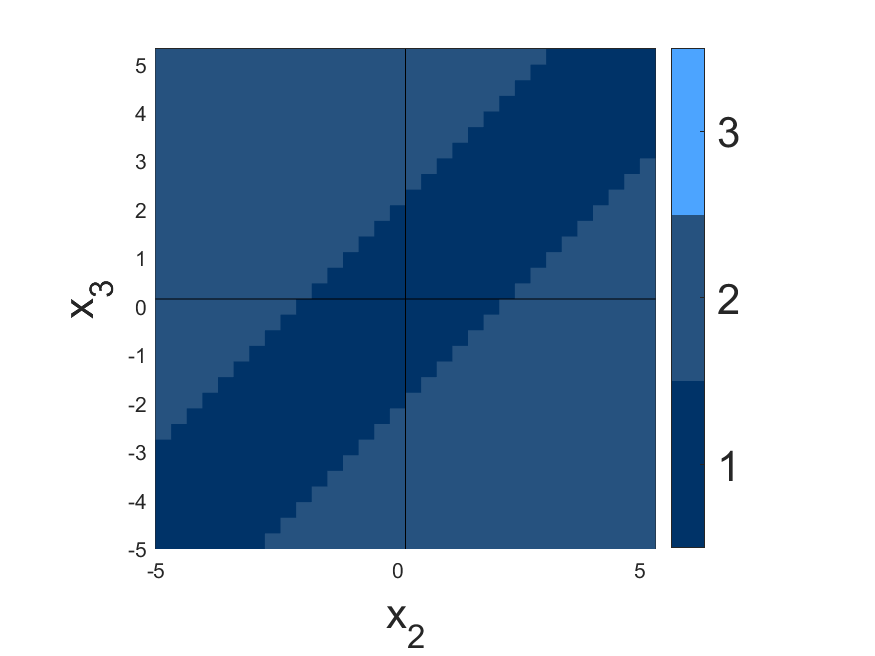
\includegraphics[width = 0.9\textwidth]{Figures/Mixtures/normal_flag_graph_n2.png}
		\caption{$K_\vect{x}$ as a function of $\vect{x} = (x_1, x_2)$, for a normal component density with fixed variance $\sigma^2 = 1$.}
		\label{fig:normal_flag_graph_n2}
	\end{figure}

	However, there is some redundancy in this plot which arises because we are using location mixtures. When using a location mixture, if the maximizing mixing distribution for $\vect{x}$ places weights $p_j$ at locations $\theta_j$, then a maximizing mixing distribution for $\vect{x} + (c, \dots, c)$ for some constant $c \in \mathbb{R}$ is simply the distribution that places weights $p_j$ at locations $\theta_j + c$. That is, shifting $\vect{x}$ by $c$ results in the maximizing mixture also shifting by $c$. A consequence of this fact is that $K_\vect{x}$ is invariant under translations of the form $\vect{x} \mapsto \vect{x} + (c, \dots, c)$.

	This suggests increasing $n$ to $3$, and fixing one of the $x_i$ while letting the other two vary. We do this by taking $\vect{x} = (0, x_2, x_3)$ with $x_2$ and $x_3$ varying across an evenly spaced grid. We do this for both a normal component density with variance $\sigma^2 = 1$ (Figure \ref{fig:normal_flag_graph}) and a Cauchy density with scale $\gamma = \sqrt{3}$ (Figure \ref{fig:cauchy_flag_graph}). We have chosen the scale of the Cauchy distribution so that it has inflection points in the same places as the normal density, namely at $x = \pm 1$. This decision is made in light of Theorem \ref{thm:n=2 inflection result} which says that for $n = 2$ and for certain component densities $f$, $K_\vect{x}$ can be determined by comparing $|x_1 - x_2|$ and the distance between the inflection points of $f$. It seems reasonable to expect that the choice of scale that makes the $n = 2$ figures identical is a good choice for comparing the effects of choosing different component densities in the $n = 3$ case.

	% One point that we wish to emphasize is that, given a component density $f$, $K$ is a function of $\vect{x}$ only. We can visualise this for small values of $n$. In Figure \ref{fig:normal_flag_graph}, we empirically found the MLE for $\vect{x} = (0,x_2,x_3)$ and recorded the number of probability masses in the maximizing mixture. We took values for $x_2$ and $x_3$ from an evenly spaced grid with $-6\leq x_2,x_3\leq 6$. We fixed $x_1 = 0$ since the shape of the maximum likelihood mixture (and therefore $K_{\vect{x}}$) depends only on the relative location of the $x_i$, not their absolute location.
	
	% \begin{figure}
	% 	\centering
	% 	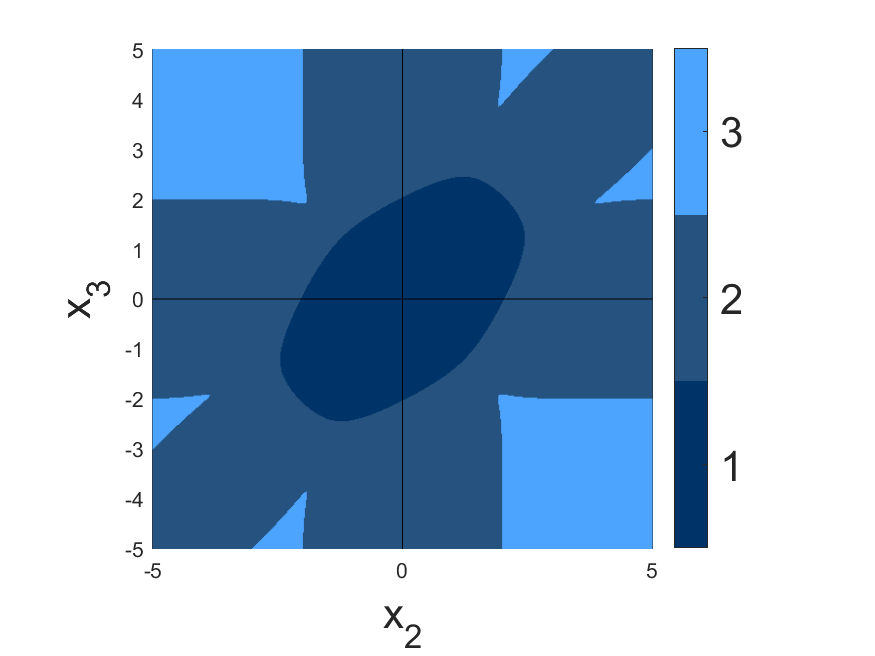
\includegraphics[width=0.9\textwidth]{normal_flag_graph.png}
	% 	\caption{$K_\vect{x}$ as a function of $\vect{x} = (0, x_2, x_3)$ for a normal component density with fixed variance $\sigma^2 = 1$.}\label{fig:normal_flag_graph}
	% \end{figure}

	% \begin{figure}
	% 	\centering
	% 	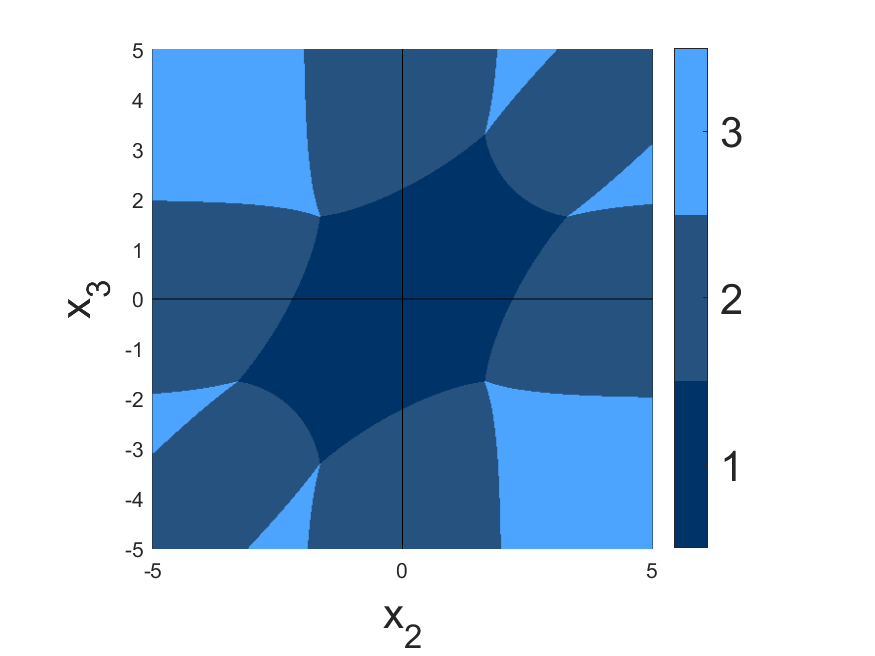
\includegraphics[width=0.9\textwidth]{cauchy_flag_graph.png}
	% 	\caption{$K_\vect{x}$ as a function of $\vect{x} = (0, x_2, x_3)$ for a Cauchy component density with fixed scale $\gamma = \sqrt{3}$.}
	% 	\label{fig:cauchy_flag_graph}
	% \end{figure}

	\begin{figure}[ht]
	\centering
		\begin{subfigure}[t]{0.49\textwidth}
			\centering
			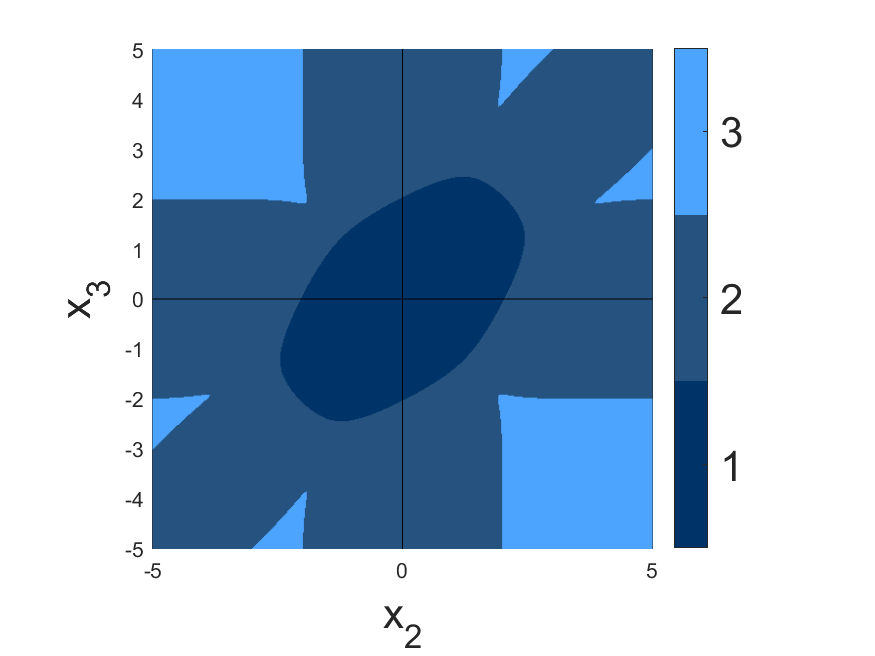
\includegraphics[width=\textwidth]{normal_flag_graph.png}
			\caption{Normal component density with fixed variance $\sigma^2 = 1$.}
			\label{fig:normal_flag_graph}
		\end{subfigure}
		\begin{subfigure}[t]{0.49\textwidth}
			\centering
			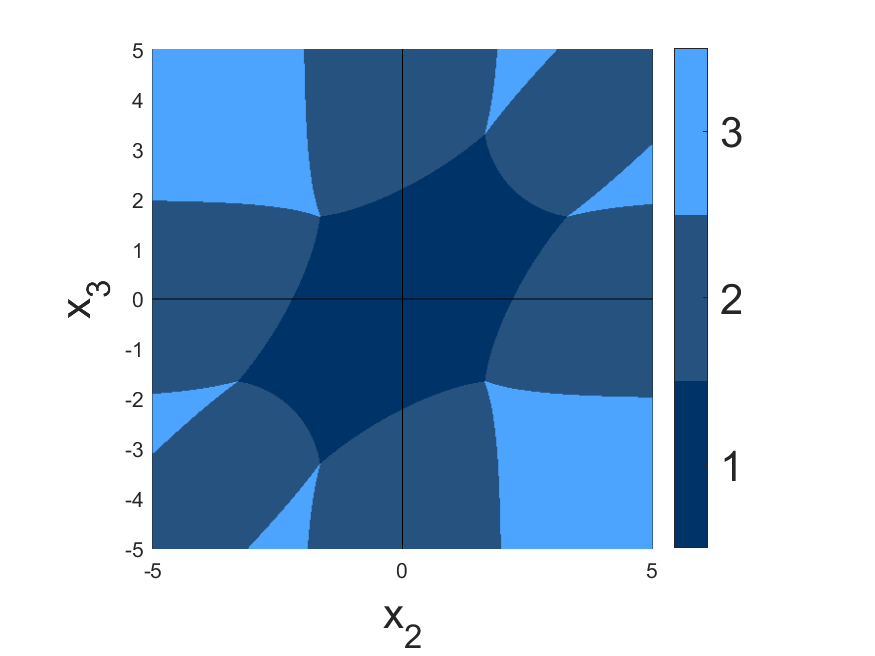
\includegraphics[width=\textwidth]{cauchy_flag_graph.png}
			\caption{Cauchy component density with fixed scale $\gamma = \sqrt{3}$.}
			\label{fig:cauchy_flag_graph}
		\end{subfigure}
		\caption{$K_\vect{x}$ as a function of $\vect{x} = (0, x_2, x_3)$ for two different component densities.}
	\end{figure}
	
	While $n = 2,3$ is not a very realistic scenario when it comes to real data to which we may wish to fit a mixture model, it does help demonstrate a particular way of thinking about the problem of determining $K_\vect{x}$. That is, that $K_\vect{x}$ is simply a function of where $\vect{x}$ lies in $\mathbb{R}^n$. For a particular choice of component density, we can partition $\mathbb{R}^n$ into sets 
	\begin{equation}
		C_k = \{ \vect{x} \in \mathbb{R}^n | K_{\vect{x}} = k \}, \hspace{40pt} k = 1,\dots,n.
		\label{eq: C_k partition sets}
	\end{equation}
	The problem of determining $K_{\vect{x}}$ is then the same as determining in which of the sets $C_k$ $\vect{x}$ lies. If $\vect{x} = \vect{X}$ is randomly chosen, then the probability that $K_\vect{X} = k$ is simply the probability that $\vect{X} \in C_k$. In Section \ref{sec:mixture results}, we present various results which bound the regions $C_k$ in various settings.

	We have attempted to compare the sizes of shapes of the sets $C_k$ for $n = 2$ for the normal and Cauchy densities in Figure \ref{fig:compare cauchy norm flag graph}. In this figure we have plotted $(K_\vect{x}^\mathrm{norm} + K_\vect{x}^\mathrm{Cauchy}) / 2$ to create the effect of overlaying Figures \ref{fig:normal_flag_graph} and \ref{fig:cauchy_flag_graph} (we suggest using these figures as reference to aid readability). We observe in this example that although $C_1^\mathrm{norm} \subset C_1^\mathrm{Cauchy}$, $C_2^\mathrm{norm}$ contains points outside of $C_2^\mathrm{Cauchy}$.


	% \subsection{Other interesting things}
	% We end our empirical results section with 

	% [PUT MORE RESULTS IN HERE]

	\begin{figure}
		\centering
		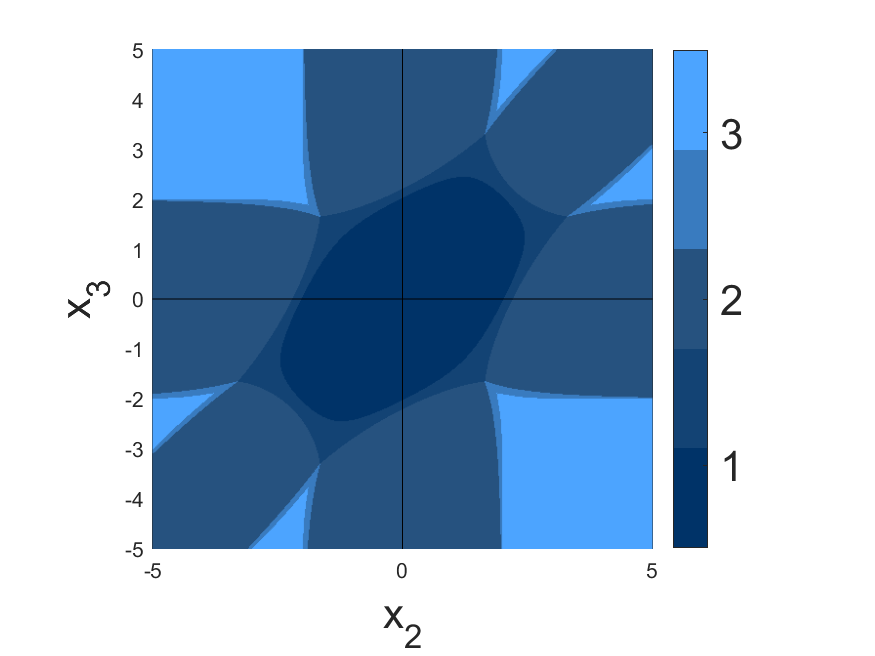
\includegraphics[width = \textwidth]{Figures/Mixtures/norm_cauchy_compare_flag_graph.png}
		\caption{$(K_\vect{x}^\mathrm{norm} + K_\vect{x}^\mathrm{Cauchy}) / 2$}
		\label{fig:compare cauchy norm flag graph}
	\end{figure}

	\section{Results}
		\label{sec:mixture results}
		The figures obtained in Section \ref{sec:empirical results}, as well as the examples in Figures \ref{fig:chi2 n500 motivation} and \ref{fig:collapsing distribution}, suggest that the bounds on $K_\vect{x}$ from Section \ref{sec:summary of Lindsay} could be significantly tightened for location mixtures. The main bounds that we have discussed so far are Theorem \ref{thm: lindsay no more than n points} which states that under mild conditions, $K_\vect{x} \leq n$; and Theorem \ref{thm:exponential family k=1 bound} which provides a sufficient condition for $K_\vect{x} = 1$ for component densities in the exponential class of densities. In this section we will present new bounds on $K_\vect{x}$ that either tighten these bounds, or extend them to different classes of component densities.

		\subsection{Results for \texorpdfstring{$n = 2$}{n = 2}}
		\label{sec:results for n = 2}
		The first bound we present is Theorem \ref{thm:n=2 inflection result} which extends Theorem \ref{thm:exponential family k=1 bound} to a different class of component densities in the case that $n=2$, and which tightens the result to be both sufficient and necessary on this class. The theorem concerns component densities, $f(x)$, which satisfy the assumptions,

		\begin{assumption}[Continuity]
		\label{assump:reallinesupport}
			The density $f(x)$ is continuous and is supported on the whole real line.
		\end{assumption}

		\begin{assumption}[Differentiability]
		\label{assump:twicediff}
			The first and second derivatives of $f(x)$ exist and are continuous.
		\end{assumption}
		
		\begin{assumption}[Unimodality]
			The density $f(x)$ has a single mode at $x=0$. That is, $f'(x) > 0$ for $x <0$, $f'(0) = 0$, and $f'(x) < 0$ for $x>0$.
			\label{assump:singlemode}
		\end{assumption}
		
		\begin{assumption}[Symmetry]
			The density $f(x)$ is symmetric about $x = 0$.
			\label{assump:symmetric}
		\end{assumption}
		
		\begin{assumption}
			The density $f(x)$ has only two points of inflection, located at $x = \pm a$.
			% For some $a > 0$, $f''(-a) = f''(a) = 0$ and these are the only zeros of $f''$.
			\label{assump:twoinflectionpoints}
		\end{assumption}

		% \begin{assumption}		
		% \label{assump:non-zero derivatives}
		% 	The derivative $f'(x)$ is non-zero for all $x \in \mathbb{R}$.
		% \end{assumption}

			
			% \begin{definition}
			% 	If $f$ satisfies assumptions \ref{assump:reallinesupport} through to \ref{assump:singlemode}, then define $[i^-,i^+]$ to be the largest interval that contains 0 and on which $f''(x) \leq 0$.
			% 	\label{def:i-i+}
			% \end{definition}
			% That is, $i^-$ and $i^+$ are inflection points of $f$. Note that for any $f$ satisfying \ref{assump:symmetric}, $i^- = -i^+$. In this case we will write $i = i^+ = -i^-$.
		
		\begin{assumption}
			The density $f(x)$ satisfies $f'(x) < -f'(x - 2a)$ for $x \in (a,\infty)$.
			\label{assump:magnitudegradients}
		\end{assumption}

		\begin{theorem}
			\label{thm:n=2 inflection result}
			Let $f(x)$ satisfy assumptions \ref{assump:reallinesupport} through to \ref{assump:magnitudegradients}. Let $\vect{x} = (x_1,x_2)$ be the sample for which we a finding a maximum likelihood location mixture using $f$ as the component density. Then 
			\begin{equation}
				K_\vect{x} = K(\vect{x};f) = 
					\begin{cases}
						1, &|x_2 - x_1| \leq 2a,\\
						2, &\text{otherwise.}
					\end{cases}
			\end{equation}
		\end{theorem}

		The proof of Theorem \ref{thm:n=2 inflection result} will be given in Section \ref{sec:proof of n=2 inflection result} after some discussion concerning how the likelihood curve behaves when $n = 2$.

		
		It is worth verifying that Assumptions \ref{assump:reallinesupport} through to \ref{assump:magnitudegradients} are satisfied by some common densities. In particular they are satisfied by the common unimodal densities in Table \ref{tab:component densities},
		% We remark here on the following common unimodal densities:
		\begin{align}
			% &\text{Normal with variance $\sigma^2$} && 
			f_\mathrm{norm}(x) &= \frac{1}{\sigma\sqrt{2\pi}} \euler^{-x^2/(2\sigma^2)},\\
			% &\text{Cauchy with scale $\gamma$} && 
			f_\mathrm{Cauchy}(x) &= \frac{1}{\pi (\gamma + x^2/\gamma)}.
			% &\text{Student's t-distribution with $\nu$ degrees of freedom} && f(x) = (1 + x^2/\nu)^{-\frac{\nu + 1}{2}}
		\end{align}
		Clearly, Assumptions \ref{assump:reallinesupport} through to \ref{assump:symmetric} are satisfied for both $f_\mathrm{norm}(x)$ and $f_\mathrm{Cauchy}(x)$.
		The inflection points of $f_\mathrm{norm}(x)$ are located at $x = \pm \sigma$ and the inflection points of $f_\mathrm{Cauchy}(x)$ are located at $x = \pm \gamma/\sqrt{3}$, satisfying Assumption \ref{assump:twoinflectionpoints}. A plot of $f_\mathrm{norm}'(x)$ against $-f_\mathrm{norm}'(x - 2\sigma)$ and of $f_\mathrm{Cauchy}'(x)$ against $-f_\mathrm{Cauchy}'(x - 2\gamma/\sqrt{3})$ in Figure \ref{fig:assumption6} makes it clear that Assumption \ref{assump:magnitudegradients} is satisfied too. Of course, one could make this rigourous if desired.

		\begin{figure}
			\centering
			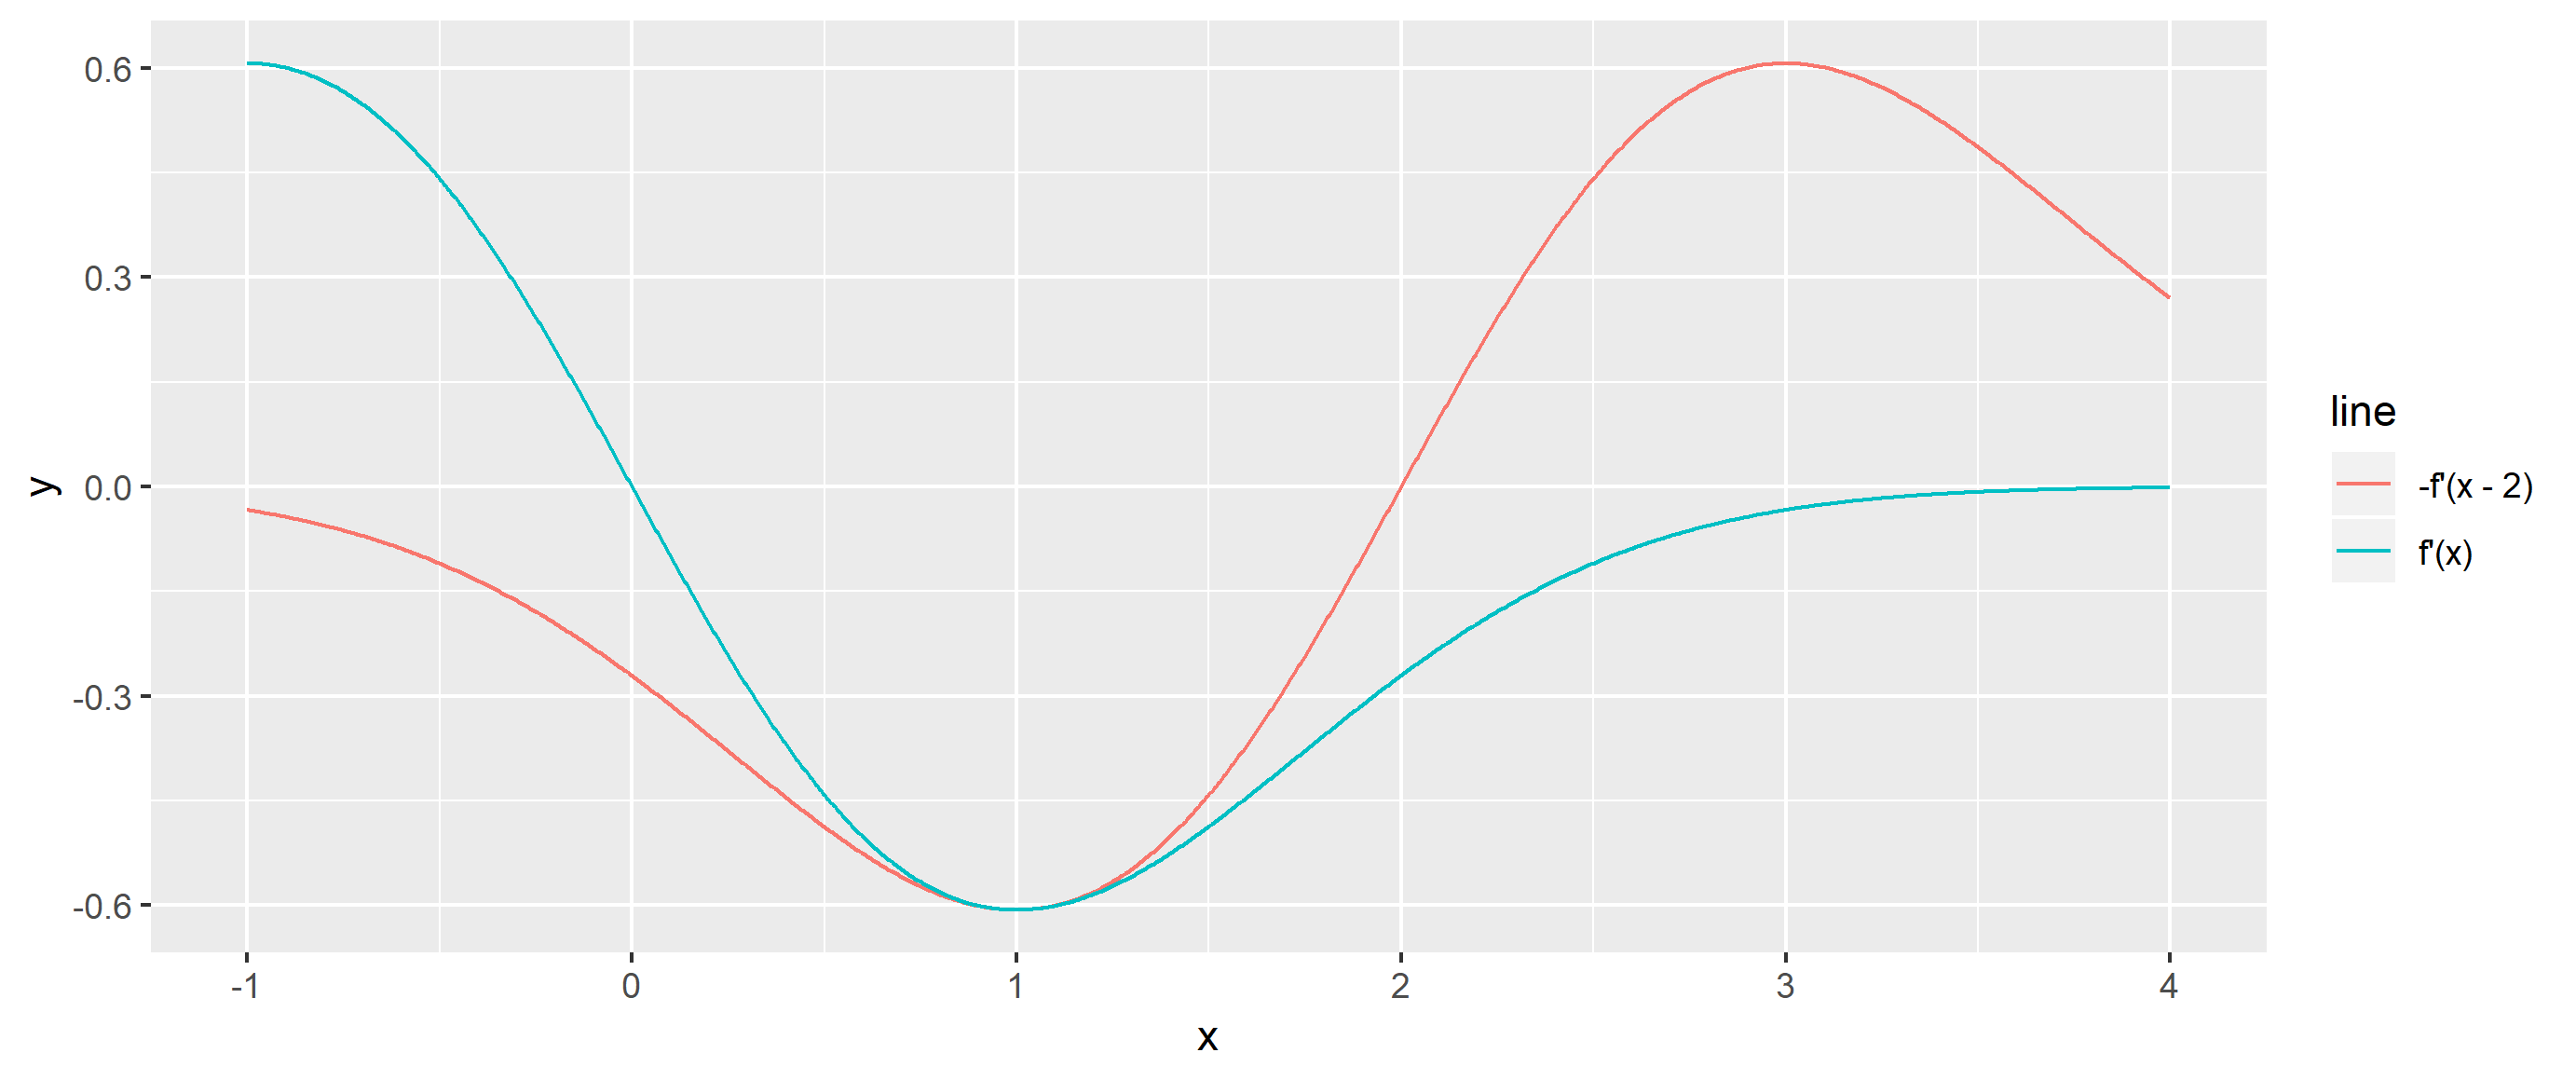
\includegraphics[width = \textwidth]{Figures/Mixtures/assumption6_normal.png}
			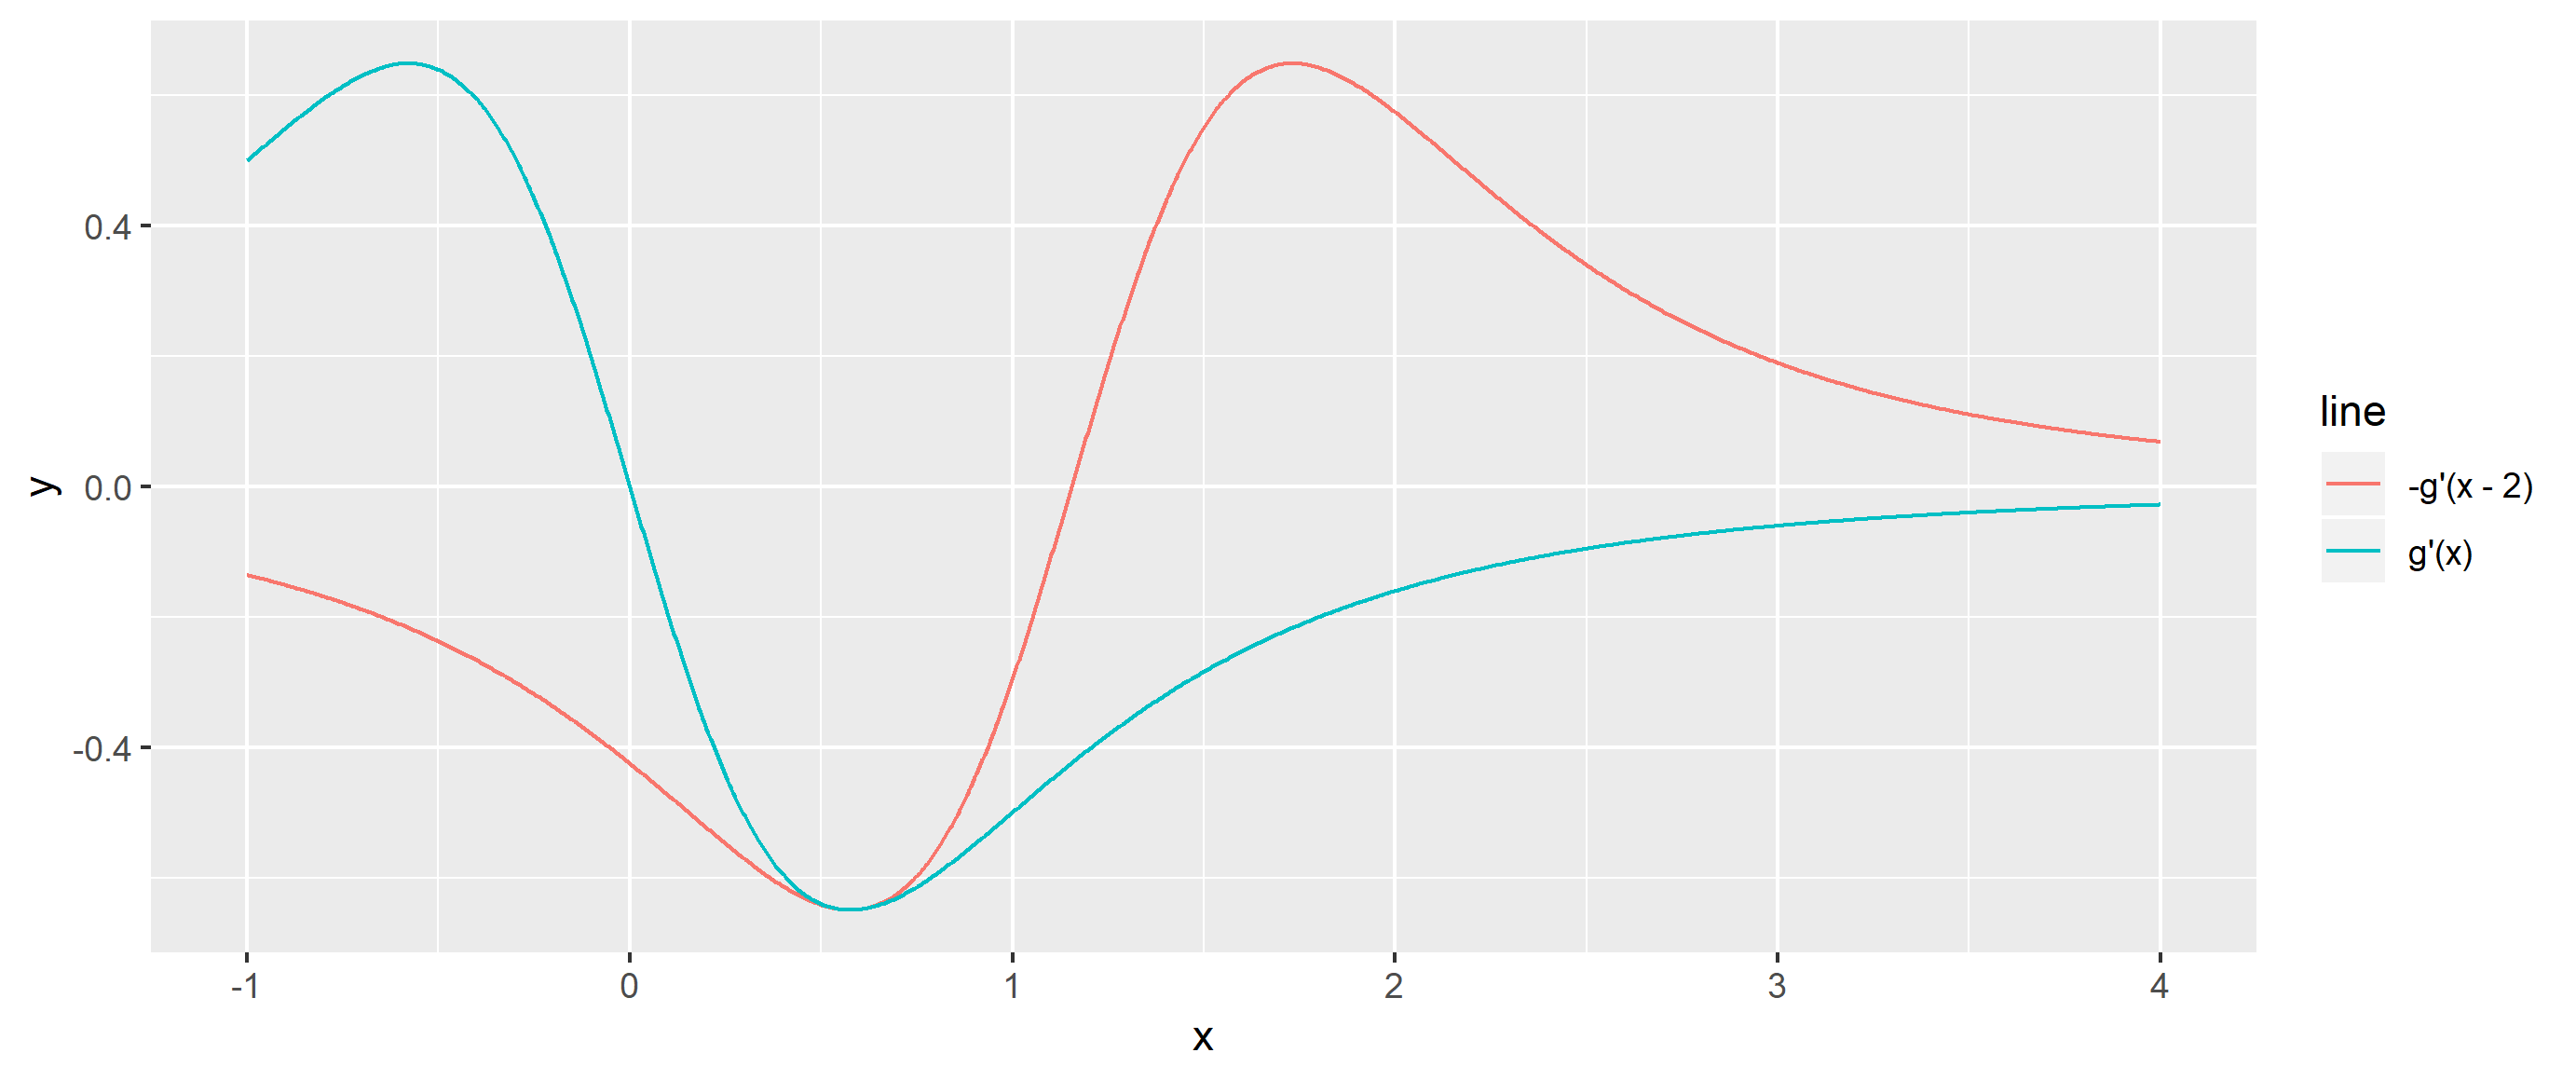
\includegraphics[width = \textwidth]{Figures/Mixtures/assumption6_cauchy.png}
			\caption{Plots of $f_\mathrm{norm}'(x)$ against $-f_\mathrm{norm}'(x - 2\sigma)$ and $f_\mathrm{Cauchy}'(x)$ against $-f_\mathrm{Cauchy}'(x - 2\gamma/\sqrt{3})$ for $\sigma = 1$ and $\gamma = 1$.}
			\label{fig:assumption6}
		\end{figure}
		% We do this in the following Lemma.

		% \begin{lemma}
		% 	The following densities satisfy Assumptions \ref{assump:reallinesupport} through to \ref{assump:magnitudegradients}:
		% 	\begin{align}
		% 		&\text{Normal with variance $\sigma^2$} && f(x) = \frac{1}{\sigma\sqrt{2\pi}} \euler^{-x^2/(2\sigma^2)}\\
		% 		&\text{Cauchy with scale $\gamma$} && g(x) = \frac{1}{\pi (\gamma + x^2/\gamma)}
		% 		% &\text{Student's t-distribution with $\nu$ degrees of freedom} && f(x) = (1 + x^2/\nu)^{-\frac{\nu + 1}{2}}
		% 	\end{align}
		% \end{lemma}
		% \begin{proof}
		% 	Clearly, Assumptions \ref{assump:reallinesupport} through to \ref{assump:symmetric} are satisfied for both $f(x)$ and $g(x)$.

		% 	The inflection points of $f(x)$ are located at $x = \pm \sigma$ and the inflection points of $g(x)$ are located at $x = \pm \gamma/\sqrt{3}$. A plot of $f'(x)$ against $-f'(x - 2\sigma)$ and of $g'(x)$ against $-g'(x - 2\sigma)$ makes it clear that Assumption \ref{assump:magnitudegradients} is satisfied too. 
		% \end{proof}

		% [DISCUSSION RELATING THEOREM TO THE LINDSAY EXPONENTIAL FAMILY ONE]

	
	
		% \begin{assumption}[Continuity]
		% 	$f(x)$ is a continuous density and has the whole real line as its support.
		% 	\label{assump:reallinesupport}
		% \end{assumption}
		
		% \begin{assumption}[Differentiability]
		% 	$f(x)$ is twice differentiable.
		% 	\label{assump:twicediff}
		% \end{assumption}
		
		% \begin{assumption}[Unimodality]
		% 	$f(x)$ has a single mode at $x=0$. I.e. $f'(x) > 0$ for $x <0$, $f'(0) = 0$, and $f'(x) < 0$ for $x>0$.
		% 	\label{assump:singlemode}
		% \end{assumption}
		
		% \begin{assumption}[Symmetry]
		% 	The density $f(x)$ is symmetric about $x = 0$.
		% 	\label{assump:symmetric}
		% \end{assumption}
		
		% \begin{assumption}
		% 	$f$ has only two points of inflection
		% 	\label{assump:twoinflectionpoints}
		% \end{assumption}
		
		% \begin{definition}
		% 	If $f$ satisfies assumptions \ref{assump:reallinesupport} through to \ref{assump:singlemode}, then define $[i^-,i^+]$ to be the largest interval that contains 0 and on which $f''(x) \leq 0$.
		% 	\label{def:i-i+}
		% \end{definition}
		% That is, $i^-$ and $i^+$ are inflection points of $f$. Note that for any $f$ satisfying \ref{assump:symmetric}, $i^- = -i^+$. In this case we will write $i = i^+ = -i^-$.
		
		% \begin{assumption}
		% 	$f'(x) > -f'(x - 2i)$ for $\theta \in (i,\infty)$
		% 	\label{assump:magnitudegradients}
		% \end{assumption}
		
		% Some common densities that satisfy these assumptions include the normal density and the Cauchy density.

		% [WHAT ABOUT IF $N>2$ AND ALL POINTS WITHIN DISTANCE 2I?]

		\subsection{Proof of Theorem \ref{thm:n=2 inflection result}}
		The proof of Theorem \ref{thm:n=2 inflection result} is based on the discussion contained in \cite[Section 4]{Lindsay1983a-he}, in which Lindsay discussed how the curvature of $\Gamma$ relates to the support points of $\hat{Q}$. The important realisation we use here is that points of support must correspond to regions of non-negative curvature of $\Gamma$.

		\label{sec:proof of n=2 inflection result}
		\begin{proof}
			% Since $f(x)$ has a single mode at $x = 0$, the points of support of the maximizing mixing distribution must lie between $x_{1}$ and $x_{2}$. Hence we are
			If $x_1 = x_2$ then clearly $K_\vect{x} = 1$. Otherwise, without loss of generality, assume $x_1 < x_2$. By the unimodality of $f$ (\ref{assump:singlemode}), the points of support of any maximizing mixing distribution, $\hat{Q}$, must lie between $x_1$ and $x_2$ \cite[Proposition 25]{Lindsay1995-sq}. Hence $\hat{\vect{\gamma}} = \vect{\gamma}(\hat{Q}, \vect{x}, f)$ must lie in the convex hull of $\Gamma^*_{\vect{x}, f} = \{\vect{\gamma}(\theta; \vect{x}, f) : \theta \in [x_1, x_2]\}$. 

			Consider the behaviour of $\vect{\gamma}(\theta; \vect{x}, f) = (f(x_1 - \theta), f(x_2 - \theta))$ as we increase $\theta$ from $x_1$ to $x_2$. Since $f(x)$ has a single mode at $x = 0$, $f(x_1 - \theta)$ is non-increasing and $f(x_2 - \theta)$ is non-decreasing along this interval. So $\vect{\gamma}(\theta;\vect{x}, f)$ crosses the line $\gamma_1 = \gamma_2$ once only and by the symmetry of $f(x)$, this occurs at $\theta = (x_1 + x_2)/2$. By Lemma \ref{lemma: maximizing point on line u = v}, we also know that $\hat{\vect{\gamma}}$ must lie on the line $\gamma_1 = \gamma_2$.

			Since $f$ is continuous and twice differentiable, $\vect{\gamma}$ traces out a continuous, smooth curve. The signed curvature
			\begin{align}
				k(\theta) = \frac{-f'(x_1 - \theta)f''(x_2 - \theta) + f'(x_2 - \theta)f''(x_1 - \theta)}{(f'(x_1 - \theta)^2 + f'(x_2 - \theta)^2)^{\frac{3}{2}}}
			\end{align}
			is defined everywhere since $f'(x)$ is zero only at $x = 0$ and so for $x_1 \neq x_2$, the denominator is non-zero everywhere. The sign of $k(\theta)$ matches the sign of
			\begin{equation}
				S(\theta) = 
				\begin{vmatrix}
					\gamma_1'(\theta;\vect{x})&\gamma_1''(\theta;\vect{x})\\
					\gamma_2'(\theta;\vect{x})&\gamma_2''(\theta;\vect{x})
				\end{vmatrix} = 
				\begin{vmatrix}
					-f'(x_1 - \theta) & f''(x_1 - \theta)\\
					-f'(x_2 - \theta) & f''(x_2 - \theta)
				\end{vmatrix}.
			\end{equation}

			Recall from Section \ref{sec: support hyperplane}, that each point of support of a maximizing mixture $\hat{Q}$, corresponds with a contact point of $\Gamma_{\vect{x}, f}$ with the support hyperplane of $\conv(\Gamma_{\vect{x}, f})$ that contains $\hat{\vect{\gamma}}$. Note that any point $\vect{\gamma}(\theta_j;\vect{x},f)$ that is in contact with a support hyperplane of $\conv(\Gamma_{\vect{x}, f})$ must have non-negative curvature.

			First, let us assume that $x_2 - x_1 > 2a$. By the symmetry of $f$, $\vect{\gamma}(\theta;\vect{x})$ crosses the $u_1 = u_2$ line at $\theta = (x_1 + x_2)/2$. At this point, the curvature of $\vect{\gamma}$ has the same sign as
			\begin{equation}
				S\left(\frac{x_1+x_2}{2}\right) = 
				\begin{vmatrix}
					-f'(\frac{x_1 - x_2}{2}) & f''(\frac{x_1 - x_2}{2})\\
					-f'(\frac{x_2 - x_1}{2}) & f''(\frac{x_2 - x_1}{2})
				\end{vmatrix}.
			\end{equation}
			Since $x_2 - x_1 > 2a$, by \ref{assump:twoinflectionpoints},  $f''((x_2 - x_1)/2)>0$. Similarly, $f''((x_1 - x_2)/2) > 0$. We also have that $-f'((x_1 - x_2)/2) < 0$ and $-f'((x_2 - x_1)/2) > 0$. Hence $S((x_1 + x_2)/2)<0$ and so $\vect{\gamma}((x_1 + x_2)/2;\vect{x})$ has negative curvature. Since $\vect{\gamma}$ has negative curvature when it crosses the line $\gamma_1 = \gamma_2$, and since $\hat{\gamma}$ lies on that line, the maximizing point $\hat{\gamma}$ must be the convex combination of at least two separate points in $\Gamma_{\vect{x},f}$ and so $K_\vect{x} = 2$.

			% By Lemma \ref{lemma: gamma has non-negative curvature at points of support} the curve $\Gamma$ cannot have negative curvature at the points of support and so we cannot have that $K_\vect{x} = 1$.
			
			Now assume that $x_2 - x_1 \leq 2a$. By Lemma \ref{lem:magnitudegradients}, there is only one point at which $\vect{\gamma}$ is pointing along the direction $(1,-1)$. Now, by the symmetry of $f$, $\Gamma_{\vect{x}, f}$ must have a line of symmetry along $\gamma_1 = \gamma_2$. Since $\hat{\vect{\gamma}}$ lies on the line $\gamma_1 = \gamma_2$ by Lemma \ref{lemma: maximizing point on line u = v}, the support line of $\Gamma_{\vect{x},f}$ that contains $\hat{\vect{\gamma}}$ must point along the direction $(1, -1)$. Each contact point of $\Gamma_{\vect{x}, f}$ with one of its support lines must be tangent to that support line. Hence, there is only one possible point of contact with the support line that contains $\hat{\vect{\gamma}}$ and so $K_\vect{x} = 1$.

			% [JUST USE SUPORT HYPERPLANE WHICH MUST BE PARALLEL TO u1 = -u2]

			% By the symmetry of $f$ this occurs when $\gamma(\theta;\vect{x})$ is crossing the line $u_1 = u_2$. Since $f$ is continuous, the direction that $\gamma(\theta;\vect{x})$ is moving is also continuous. At $\theta = x_1$, $\gamma(\theta;\vect{x})$ is pointing straight up and so we have that for $\theta \in [x_1,(x_1 + x_2)/2]$, $\gamma(\theta;\vect{x})$ is travelling in a direction pointing above the line perpendicular to $u_1 = u_2$. For $\theta \in [(x_1 + x_2)/2,x_2]$, $\gamma(\theta;\vect{x})$ points below the line. It is now obvious that $\gamma((x_1 + x_2)/2;\vect{x})$ is the furthest point from the origin that lies on $u_1 = u_2$ and is in the convex hull of $\Gamma_\vect{x}$. Since the likelihood increases as we move away from the origin along the line $u_1 = u_2$ in the positive quadrant, we must have
			% $$\hat{\vect{u}} = \gamma((x_1 + x_2)/2;\vect{x})$$
			% and so $K_\vect{x} = 1$.
			
			% Basic idea just here - 		
			% Now either made up of two points or lies on $\Gamma_\vect{x}$. If made up of two points then these two points are symmetrical about $u_1 = u_2$ and the part of $\Gamma_\vect{x}$ that crosses $u_1 = u_2$ is closer to origin. However, if angle of $\gamma$ is always above angle that is perpendicular to $u_1 = u_2$ before crossing $u_1 = u_2$ then impossible for point where it crosses to be closer to origin than that of line between any two symmetrical points.
		\end{proof}

		\begin{lemma}
		\label{lemma: maximizing point on line u = v}
			Let $f(x)$ be a component density symmetric around $x = 0$, and $\vect{x} = (x_1, x_2) \in \mathbb{R}^2$ such that the conditions of Theorem \ref{thm: lindsay maximizing likelihood vector point} are met. Let $\hat{Q}$ maximise the likelihood, $l(Q; \vect{x}, f)$. Then $f_{\hat{Q}}(x_1) = f_{\hat{Q}}(x_2)$.
		\end{lemma}
		\begin{proof}
			Let $(u, v)$ denote the coordinates of $\hat{\vect{\gamma}}  = (f_{\hat{Q}}(x_1), f_{\hat{Q}}(x_2))$. By Theorem \ref{thm: lindsay no more than n points} we have
			\begin{align}
				(u, v) &= p \vect{\gamma}(\theta_1; \vect{x}, f) + (1 - p) \vect{\gamma}(\theta_2;\vect{x}, f)\\
					&= p (f(x_1 - \theta_1), f(x_2 - \theta_1)) + (1 -p) (f(x_1 - \theta_2), f(x_2 - \theta_2))
			\end{align}
			for some choice of $p \in (0, 1]$, and $\theta_1, \theta_2 \in \mathbb{R}$. By the symmetry of $f(x)$, $f(x) = f(-x)$ and so
			\begin{align}
				u &= p f(x_1 - \theta_1) + (1 - p)f(x_1 - \theta_2)\\
					&= p f(\theta_1 - x_1) + (1 - p)f(\theta_2 - x_1)\\
					&= p f(x_2 - [x_1 + x_2 - \theta_1]) + (1 - p) (f(x_2 - [x_1 + x_2 - \theta_2])
			\end{align}
			and likewise
			\begin{align}
				v &= p f(x_1 - [x_1+x_2 - \theta_1]) + (1 - p) f(x_1 - [x_1 + x_2 - \theta_2]).
			\end{align}
			Hence the point $(v, u)$ can be written as
			\begin{align}
				(v, u) = p \vect{\gamma}(x_1 + x_2 - \theta_1;\vect{x}, f) + (1 - p) \vect{\gamma}(x_1 + x_2 - \theta_2;\vect{x}, f),
			\end{align}
			and so $(v, u) \in \conv(\Gamma_{\vect{x}, f})$.
			Since both $(u, v), (v, u) \in \conv(\Gamma_{\vect{x}, f})$, we must have that $\frac{1}{2}(u+v, u + v) \in \conv(\Gamma_{\vect{x}, f})$. Now
			\begin{align}
				\mathcal{L}\left(\frac{1}{2}(u+v, u + v)\right) &= 2\ln((u+v)/2)\\
					&= \ln\left(\left(\frac{u+v}{2}\right)^2\right)\\
					&\geq \ln(uv)\\
					&= \mathcal{L}(u,v).
			\end{align}
			However, $(u, v) = \hat{\vect{\gamma}}$, which by Theorem \ref{thm: lindsay maximizing likelihood vector point} is the unique maximizing point of $\mathcal{L}$ in $\conv(\Gamma_{\vect{x}, f})$. Hence $(u, v) = \frac{1}{2}(u+v, u+v)$ and so $u = v$.
		\end{proof}

		% \begin{lemma}
		% \label{lemma: gamma has non-negative curvature at points of support}
		% 	If $f(x)$ satisfies some stuff then the points of support can only be where the curvature is non-negative.
		% \end{lemma}
		% \begin{proof}
		% 	[DO PROOF]
		% \end{proof}

		\begin{lemma}
			\label{lem:magnitudegradients}
			% Prove stuff about magnitude of gradients (i.e. $\gamma_x < \gamma_y$)
			Let $f(x)$ be a density which satisfies assumptions \ref{assump:reallinesupport} through to \ref{assump:magnitudegradients} and whose inflection points are at $x=a$ and $x=-a$. If 
			$x_2 - x_1 < 2a$ ($x_2 > x_1$) then the equation
			\begin{equation}
				-f'(x_1 - \theta) = f'(x_2 - \theta)
				\label{eq:gradientsequal}
			\end{equation}
			has only one solution.
		\end{lemma}
		\begin{proof}
			We first consider the shape of $f'(x)$. Assumption \ref{assump:singlemode} tells us that $f'(x)$ is positive for $x<0$ and negative for $x>0$. 
			From Assumption \ref{assump:twoinflectionpoints}, the function $f'(x)$ will have turning points at $\pm a$ and these will be the only turning points.
			% From Assumption \ref{assump:twoinflectionpoints}, its derivative, $f''(x)$, satisfies $f''(-a) = f''(a) = 0$ and these are the only zeros of $f''$.
			Hence we have the following picture of $f'(x)$:
			\begin{equation}
				f'(x) \text{ is } 
				\begin{cases}
					\text{positive and increasing,} &x \in (-\infty,-a)\\
					\text{positive and decreasing,} &x \in (-a,0)\\
					\text{negative and decreasing,} &x \in (0,a)\\
					\text{negative and increasing,} &x \in (a,\infty).
				\end{cases}
			\end{equation}
			We also note, from \ref{assump:symmetric}, that $f'(x)$ is an odd function. Using this and rearranging \eqref{eq:gradientsequal} we obtain the equivalent equation
			\begin{equation}
				g(\theta) = h(\theta)
				\label{eq:gradientsequalequivalent}
			\end{equation}
			where we have put $g(\theta) = f'(\theta)$ and $h(\theta) = -f'(\theta - (x_2 - x_1))$ for ease of notation.
			% We now make the assumption that $0<x_2 - x_1<2i$
			% Since $x_2 > x_1$, the right hand side of \eqref{eq:gradientsequalequivalent} is $-f'(x)$ translated to the right by $x_2 - x_1$. Since $x_2 - x_1 < 2i$, the positive turning point of $-f'(\theta - (x_2 - x_1))$ satisfies
			% \begin{equation}
			% -i + x_2 - x_1 < i,
			% \end{equation}
			% that is, it comes before the positive turning point of $f'(\theta)$.
			
			If we assume that $0< x_2 - x_1 < 2a$ then we can consider possible solutions to \eqref{eq:gradientsequalequivalent} on each of the following intervals. 
			
			For $\theta \in (-\infty, 0]$, $g(\theta)\geq 0$ and $h(\theta) < 0$ and so there are no possible solutions.
			
			Likewise, for $\theta \in [x_2 - x_1,\infty)$, $g(\theta)<0$ and $h(\theta) \geq 0$ and so there are no possible solutions.
			
			For $\theta \in [-a + x_2 - x_1, a]$, $g(\theta)$ is decreasing and $h(\theta)$ is increasing and $h(-a +x_2 -x_1) = g(a)$ (since $f'$ is odd). Therefore there must be exactly one solution in this interval.
			
			We note that if $x_2 - x_1 \leq a$ then the above intervals cover the real line. In the case that $a <x_2 - x_1 < 2a$ we need to consider additional intervals.

			For $\theta \in (a,x_2 - x_1)$, from assumption \ref{assump:magnitudegradients}, $f'(\theta) < -f'(\theta - 2a) < -f'(\theta - (x_2 - x_1))$ since both $-f'(\theta - 2a)$ and $-f'(\theta - (x_2 - x_1))$ are increasing on this interval. Hence there can be no solutions to \eqref{eq:gradientsequalequivalent} on this interval.
			
			For $\theta \in (0, -a+x_2 - x_1)$ we can again use assumption \ref{assump:magnitudegradients} by observing that since 
			\begin{equation}
				f'(\theta) < -f'(\theta - 2a)
			\end{equation}
			for $\theta \in (a, \infty)$, we also have that for $\theta \in (-\infty, -a)$
			\begin{equation}
				f'(-\theta) < -f'(-\theta - 2a)
			\end{equation}
			and so for $\theta \in (-\infty, a)$,
			\begin{equation}
				f'(-\theta + 2a) < -f'(-\theta)
			\end{equation}
			which, since $f'$ is odd, is equivalent to 
			\begin{equation}
				-f'(\theta - 2a) < f'(\theta).
			\end{equation}

			So for $\theta \in (0,-a+x_2-x_1)$,  $f'(\theta)>-f'(\theta - 2a) > -f'(\theta - x_2 - x_1)$ and there are no solutions to \eqref{eq:gradientsequalequivalent} on this interval either.
			
			Since the above intervals cover the real line and since we have shown that there is only one solution in one of these intervals, \eqref{eq:gradientsequal} must have only one solution.
		\end{proof}

	\subsection{Results for general \texorpdfstring{$n$}{n}}
	\label{sec: results for general n}
	To obtain results for $n \geq 2$ we now restrict our component density to be normal with fixed variance $\sigma^2$. In this case, we can make use of the gradient function defined in Section \ref{sec: gradient characterization} and equations, \eqref{eq:Deq1} to \eqref{eq:Deq3}, which must be satisfied at a maximizing mixture.

	When our component density is normal with variance $\sigma^2$, that is
	\begin{equation}
		f_\sigma(x) = \frac{1}{\sigma \sqrt{2\pi}} \euler^{-x^2/2\sigma^2},
	\end{equation}
	the gradient function defined in \eqref{eq:def gradient function}, evaluated at a mixture $Q$ which places masses $\vect{p}$ at locations $\vect{\theta}$, becomes
	\begin{equation}
		D_Q(\theta; \vect{x}, f_\sigma) = - n + \sum_{i = 1}^n \frac{\exp({-(x_i - \theta)^2/2\sigma^2})}{\sum_{j=1}^m p_j \exp({-(x_i - \theta_j)^2/2\sigma^2})}.
	\end{equation}
	% where we have written
	% \begin{equation}{}
	% 	\Gamma_k(x;\vect{\theta},\vect{p}) = \frac{f(x - \theta_k;\sigma)}{\sum_{j=1}^m p_j f(x - \theta_j;\sigma)}.
	% \end{equation}
	% for ease of notation. Using this notation, equations \eqref{eq:Deq1} to \eqref{eq:Deq3} become
	Equations \eqref{eq:Deq1} to \eqref{eq:Deq3} state that at a maximizing mixture $\hat{Q}$, 
	\begin{align}
		&\frac{1}{n} \sum_{i=1}^n \Psi_k(x_i;\hat{\vect{\theta}},\hat{\vect{p}}) = 1, &&k = 1,\dots, m, \label{eq:PsiEq1}\\
		&\frac{1}{n} \sum_{i=1}^n x_i \Psi_k(x_i;\hat{\vect{\theta}},\hat{\vect{p}}) = \theta_k, &&k = 1,\dots, m,\label{eq:PsiEq2}\\
		&\frac{1}{n} \sum_{i=1}^n (x_i - \theta_k)^2 \Psi_k(x_i;\hat{\vect{\theta}},\hat{\vect{p}}) \leq \sigma^2, &&k = 1,\dots, m,
		\label{eq:PsiEq3}
	\end{align}
	where $\hat{\vect{\theta}}$ and $\hat{\vect{p}}$ are the locations and masses of $\hat{Q}$ and we have written
	\begin{equation}{}
		\Psi_k(x;\vect{\theta},\vect{p}) = \Psi_k(x;\vect{\theta},\vect{p}, f_\sigma) = \frac{f_\sigma(x - \theta_k)}{\sum_{j=1}^m p_j f_\sigma(x - \theta_j)}
	\end{equation}
	for ease of notation. 

	We will show that these three equations constrain the regions $C_1, \dots, C_n$ as defined in \eqref{eq: C_k partition sets}. This will be done in Theorem \ref{thm:general n constraints result}. However, as a gentle introduction, we will start with the much simpler problem of just bounding $C_1$.

	\begin{theorem}
		\label{thm:general n C1 bound}
		If $\vect{x} \in C_1$ then 
		\begin{equation}
			\frac{1}{n} \sum_{i=1}^n (x_i - \bar{\vect{x}})^2 \leq \sigma^2,
		\end{equation}
		where 
		\begin{equation}
			\bar{\vect{x}} = \frac{1}{n}\sum_{i = 1}^n x_i.
		\end{equation}
	\end{theorem}
	\begin{proof}
		If $\vect{x} \in C_1$ then the maximizing mixture has one component and so $\Psi_1(x; \vect{\theta}, \vect{p}) = 1$. Then \eqref{eq:PsiEq2} gives us that $\theta_1 = \bar{\vect{x}}$ and combining this with \eqref{eq:PsiEq3} completes the proof.
	\end{proof}
	In Figure \ref{fig:flag graph m1 bound} we compare the bound above to the `flag graphs' we produced in section \ref{sec: flag graphs}.

	\begin{figure}
		\centering
		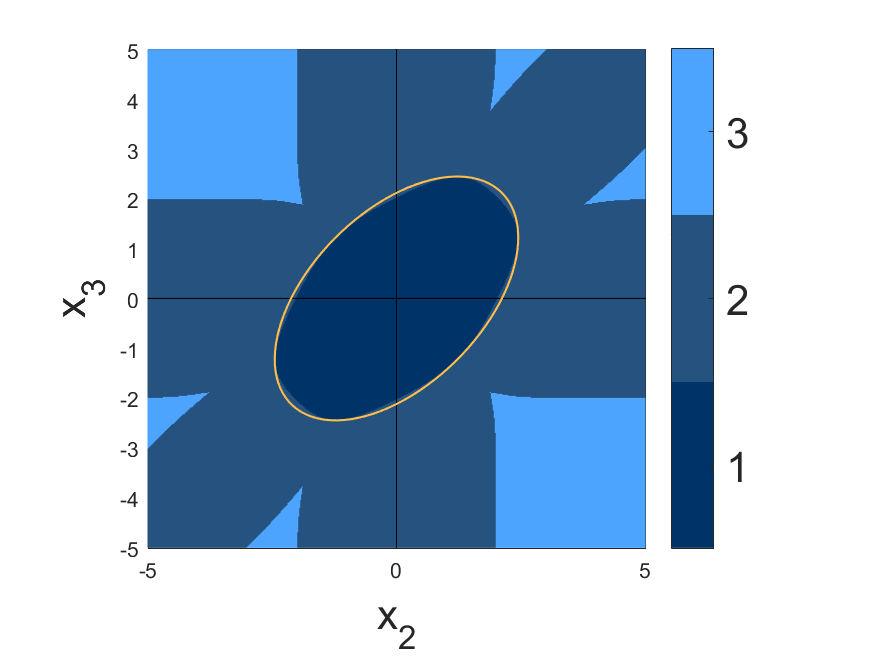
\includegraphics[width = \textwidth]{Figures/Mixtures/normal_flag_graph_m1_bound.png}
		\caption{The bound obtained in Theorem \ref{thm:general n C1 bound} tells us that $C_1$ must lie within the orange ellipse. The true shape of $C_1$ is given by the dark blue region.}
		\label{fig:flag graph m1 bound}
	\end{figure}

		% From Theorem \ref{thm:shapeofC1normalb}, an lower bound to $\prob(\vect{x} \in C_1)$ is
		% \begin{align*}
		% p_l &= \prob(x_{(n)} - x_{(1)} < 2\sigma)\\
		% 	&\geq \prob(\mu - \sigma < x_{(1)} < x_{(n)} < \mu + \sigma )\\
		% 	&=  \left(\int_{\mu - \sigma}^{\mu + \sigma} f(x) \intd x \right)^n\\
		% 	&= \left( \erf\left(\frac{\sigma_2}{\sqrt{2}\sigma_1}\right)\right)^n
		% \end{align*}

	
	% \subsection{Bounding \texorpdfstring{$C_m$}{Cm}}
	We now state a generalisation of Theorem \ref{thm:general n C1 bound} that bounds the regions $C_1, \dots, C_n$.

	\label{sec:bounding Cm}
		\begin{theorem}
			If $\vect{x} \in C_m$ for some $m \leq n$, then there exists a subset of the $x_i$, $A$, such that $A$ contains at least $n/m$ elements and
			\begin{equation}
				\frac{1}{n} \sum_{i \in A} \left(x_i - \bar{x}_A\right)^2 \leq \sigma^2,
			\end{equation}
			where
			\begin{equation}
				\bar{x}_A = \frac{1}{|A|}\sum_{i \in A} x_i.
			\end{equation}
			\label{thm:general n constraints result}
		\end{theorem}
		\begin{proof}
			Let $\hat{\vect{\theta}}$ and $\hat{\vect{p}}$ represent an $m$ point maximizing mixture of $\vect{x} \in C_m$. By Lemma \ref{lem:maxkGamma} below, for every $i \in \{1, \dots, n\}$ there exists a $k \in \{1, \dots, m\}$ such that $\Psi_{k}(x_i;\hat{\vect{p}},\hat{\vect{\theta}}) \geq 1$. Therefore by the pigeonhole principle there must exists some $k^*$ such that $\Psi_{k^*}(x_i;\hat{\vect{p}},\hat{\vect{\theta}}) \geq 1$ for at least $n / m$ different $i$. Define the set
			\begin{equation}
			 	A_{k^*} = \{i : \Psi_{k^*}(x_i;\hat{\vect{p}},\hat{\vect{\theta}}) \geq 1 \},
			\end{equation}
			which we know must have size $|A_{k^*}| \geq n/m$.
			% Let $\vect{x} = (x_1,\dots,x_n)$ and assume that the maximum likelihood mixture for $\vect{x}$ has no more than $m$ components. Let $\hat{\vect{\theta}}$ and $\hat{\vect{p}}$ denote this maximizing mixture. %Let $\hat{\vect{\theta}} = (\hat{\theta}_1,\dots,\hat{\theta}_m)$ and $\hat{\vect{p}} = (\hat{p}_1,\dots,\hat{p}_m)$ be a maximizing mixture for $\vect{x}$
			% Then by Lemma \ref{lem:maxkGamma}, there exists a $k^*$ such that $\Psi_{k^*}(x_i;\hat{\vect{p}},\hat{\vect{\theta}}) \geq 1$ for at least $\lceil \frac{n}{m} \rceil$ different $x_i$. Let $A_{k^*}$ be the set of all these $x_i$. 

			% Let $A_{\theta_{k^*}}$ be the set of the $|A_{k^*}|$ closest $x_i$ to $\theta_{k^*}$. 

			From \eqref{eq:PsiEq3},
			\begin{align}
				\sigma^2 &\geq \frac{1}{n} \sum_{i=1}^n (x_i - \theta_{k^*})^2 \Psi_{k^*}(x_i; \hat{\vect{\theta}}, \hat{\vect{p}})\\ 
					&\geq \frac{1}{n} \sum_{i \in A_{k^*}} (x_i - \theta_{k^*})^2 \Psi_{k^*}(x_i; \hat{\vect{\theta}}, \hat{\vect{p}})\\
					&\geq \frac{1}{n} \sum_{i \in A_{k^*}} (x_i - \theta_{k^*})^2,
					\label{eq:sum A_k^star x_i - theta}
					% &\geq \frac{1}{n} \sum_{i \in A_{\theta_{k^*}}} (x_i - \theta_{k^*})^2 \\
					% &\geq \frac{1}{n} \sum_{i \in A_{k^*}} \left(x_i - \bar{x}_{A_{k^*}}\right)^2.
			\end{align}
			since $\Psi_{k^*}(x_i;\hat{\vect{p}},\hat{\vect{\theta}}) \geq 1$ for all $i \in A_{k^*}$. Finally, we can reduce \eqref{eq:sum A_k^star x_i - theta} by replacing $\theta_{k^*}$ with $\bar{x}_{A_{k^*}}$ to get that
			\begin{equation}
				\sigma^2 \geq \frac{1}{n} \sum_{i \in A_{k^*}} \left(x_i - \bar{x}_{A_{k^*}}\right)^2.
			\end{equation}
			% From \eqref{eq:PsiEq3},
			% \begin{equation}
			% 	\frac{1}{n} \sum_{i \in A_{\theta_{k^*}}} \left(x_i - \bar{x}_{A_{\theta_{k^*}}}\right)^2 \leq \sigma^2.
			% \end{equation}
		\end{proof}

		% This means that if we cannot find a subset of the $x_i$ that has at least $\frac{n}{m}$ elements and has (biased) variance less than $\frac{n\sigma^2}{\left\lceil \frac{n}{m} \right\rceil}$ then we need more than $m$ components in our maximum likelihood mixture.
	% \subsection{Properties of \texorpdfstring{$\Psi$}{Psi}}
	% 	% In order to obtains bounds on the regions $C_2, \dots, C_n$, we will need to get a handle on the behaviour of $\Psi_k(x;\vect{\theta}, \vect{p})$. 
	% 	This section contains statements and proofs of Lemmas concerning the properties of $\Psi$ that are used in the proof of Theorem \ref{thm:general n constraints result}.

		The bound for the $C_2$ region given by Theorem \ref{thm:general n constraints result} is compared to the `flag graphs' from Section \ref{sec: flag graphs} in Figure \ref{fig:flag graph m2 bound}. We observe that the bound does not appear as tight as the one bounding $C_1$.

		\begin{figure}
			\centering
			\includegraphics{Figures/Mixtures/normal_flag_graph_m2_bound.png}
			\caption{The bound obtanied in Theorem \ref{thm:general n constraints result} tells us that $C_2$ must lie between the pairs of parallel orange lines. The true shape of $C_2$ is given by the middle blue shaded region.}
			\label{fig:flag graph m2 bound}
		\end{figure}

		\begin{lemma}
		\label{lem:maxkGamma}
		Let $f$ be a density supported on all of $\mathbb{R}$. For all $x \in \mathbb{R}$, and all discrete probability distributions with masses $\vect{p}$ at locations $\vect{\theta}$,
			\begin{equation}
				\max_k \left[ \Psi_k(x;\vect{p},\vect{\theta},f) \right] \geq 1.
			\end{equation}
		\end{lemma}	
		\begin{proof}
			Let $x \in \mathbb{R}$, and $\vect{\theta},\vect{p}$ be the locations and weights respectively of an $m$ point discrete probability distribution. Choose $\theta_{k^*}$ to be the smallest $\theta_j$ that satisfies
			\begin{align}
				f(x - \theta_{k^*}) &\geq f(x - \theta_j) && j = 1, \dots, m.
			\end{align}
			(We choose the smallest in case there is more than one $\theta_j$ which satisfies the above). Then
			\begin{equation}
				\Psi_{k^*}(x;\vect{p},\vect{\theta},f) = \frac{f(x - \theta_{k^*})}{\sum_{j=1}^m p_j f(x - \theta_j)} \geq \frac{f(x - \theta_{k^*})}{\sum_{j=1}^m p_j f(x - \theta_{k^*})} = 1.
			\end{equation}
		\end{proof}

		% \begin{lemma}
		% 	\begin{equation}
		% 	\Psi_k(x;\vect{p},\vect{\theta}) \leq \frac{1}{p_k}
		% 	\end{equation}
		% \end{lemma}
		% \begin{proof}
		% 	Since $f(x) > 0$,
		% 	\begin{equation}
		% 		\Psi_k(x;\vect{p},\vect{\theta}) = \frac{f(x - \theta_k;\sigma)}{\sum_{j=1}^m p_j f(x - \theta_j;\sigma)} \leq \frac{f(x - \theta_k;\sigma)}{p_k f(x - \theta_k;\sigma)} = \frac{1}{p_k}.
		% 	\end{equation}
		% \end{proof}

		% \begin{lemma}
		% 	Let $\gamma(x)$ be a non-negative function that satisfies
		% 	\begin{equation}
		% 		\frac{1}{n} \sum_{i=1}^n \gamma(x_i) = 1.
		% 	\end{equation}

		% 	Then the $\theta$ that minimizes 
		% 	\begin{equation}
		% 		\frac{1}{n} \sum_{i=1}^n (x_i - \theta)^2 \gamma(x_i)
		% 	\end{equation}
		% 	is
		% 	\begin{equation}
		% 		\theta = \frac{1}{n} \sum_{i=1}^n x_i \gamma(x_i).
		% 	\end{equation}
		% \end{lemma}
		% \begin{proof}
		% 	CURRENTLY UNUSED. PROOF IN TIM'S NOTEBOOK.
		% \end{proof}

	\subsection{Treating \texorpdfstring{$\vect{x}$}{x} as random}

		Up until now, we have treated $\vect{x}$ as fixed, not random, and treated the maximum likelihood problem purely as an optimization one, rather than a statistical one. However, for this section we consider a random sample
		\begin{equation}
			\vect{X} = (X_1, \dots, X_n)
		\end{equation}
		where the $X_i$ are i.i.d. with normal distribution 
		\begin{equation}
			X_i \sim N(\mu, \sigma_1^2).
		\end{equation}
		Given a component density, we may consider the probabilities
		\begin{align}
			&\prob[\vect{X} \in C_m],	&&m = 1,\dots,n.
		\end{align}
		
		\begin{theorem}
		\label{thm:probability in C1}
			Let the component density with which we are finding a maximum likelihood location mixture be normal with variance $\sigma_2^2$. Then 
			\begin{equation}
				\prob[\vect{X} \in C_1] \leq \prob\left(\chi_{n-1}^2 \leq \frac{n \sigma_2^2}{\sigma_1^2}\right)
			\end{equation}
			where $\chi_{n-1}^2$ is chi-squared with $n-1$ degrees of freedom.
		\end{theorem}
		\begin{proof}
			From Theorem \ref{thm:general n C1 bound},
			\begin{align}
			\prob\left(\vect{X} \in C_1 \right) &\leq \prob \left( \sum_{i=1}^n (X_i - \bar{\vect{X}})^2 \leq n \sigma_2^2  \right) \\
				&= \prob\left( \frac{1}{\sigma_1^2}\sum_{i=1}^n (X_i - \bar{\vect{X}})^2 \leq \frac{n \sigma_2^2}{\sigma_1^2}\right)\\
				% &= \prob\left( \frac{s^2}{\sigma_1^2} \leq \frac{n \sigma_2^2}{\sigma_1^2}\right)\\
				&= \prob\left(\chi_{n-1}^2  \leq \frac{n \sigma_2^2}{\sigma_1^2} \right).
			\end{align}
		\end{proof}

		Theorem \ref{thm:probability in C1} is of particular interest when the $\sigma_1 = \sigma_2$. In this case, our mixture can select the `true' number of components, which will happen if $\vect{X} \in C_1$. The probability of this occurring satisfies
		\begin{align}
			\prob\left(\vect{X} \in C_1\right) &\leq \prob\left(\chi_{n-1}^2 \leq n\right)
		\end{align}
		which converges to $1/2$ as $n \rightarrow \infty$. This is a simple proof that the number of components chosen by a normal location mixture is not a consistent estimator for the true number of components.

		Similar results to this have already been discovered. In \cite{Hartigan1985-wn}, Hartigan considered the mixture 
		\begin{equation}
			(1 - p)N(0,1) + pN(\theta, 1)
		\end{equation}
		and showed that the likelihood ratio between $\theta = 0$ and $\theta \neq 0$ converges to $\infty$ as $n \rightarrow \infty$. Also related is the result \cite{Leroux1992-ek} that certain penalised likelihoods do not underestimate the true number of components (and so it is reasonable to expect that the unpenalised likelihood might overestimate the true number of components).

		% [SOMETHING RELATED TO RESULT FOR N = 2?]
		%I.E. we can calculate the exact probability for $x \in C_1$ when n = 2... could compare this

		In this section, we have taken advantage of the simple form that the gradient function and its derivatives take when the component density is normal. One might consider using equations \eqref{eq:Deq1} through \eqref{eq:Deq3} to find analogous results for the Cauchy density (which we considered in Section \ref{sec:results for n = 2}) or other densities outside of the normal family. However, we found that the derivatives of the gradient function were too complex to be able generalise these results to other component densities.

	% \subsection{Derive Constraints again}
	% WE SHOULD BE ABLE TO DERIVE \eqref{eq:PsiEq1} THROUGH \eqref{eq:PsiEq3} AGAIN USING THEOREM \ref{thm:solution in interior}.

% \section{Other Results}


	% \subsection{Discussion about what we hope to acheive}
	% 	The few original results above (Theorems \ref{thm:n=2 inflection result} and \ref{thm:general n constraints result}) seem to be special cases of what looks to be a much more general rule. Theorem \ref{thm:general n constraints result} seems to be too large by a factor of $m$ when you compare to numerics, and the distance between inflection points in Theorem \ref{thm:n=2 inflection result} seems to come up again when when you look at images like Figure \ref{fig:normal_flag_graph} (eg the thickness of the `bands' is this distance). It is therefore our hope that we can either generalize or add significantly to the Theorems stated so far.

	% \subsection{Final Observation}
	% [EXTRA STUFF]

	% ``The result follows from this general theorem which seems obvious.''

	% \begin{theorem}
	% 	\label{thm:solution in interior}
	% 	Let $(E_m)_{m=1}^\infty$ be a sequence of subsets of topological spaces and let $(g_m)_{m=1}^\infty, g_m: E_m \mapsto \mathbb{R}$ be a sequence of	functions that satisfy the following properties
	% 	\begin{enumerate}
	% 		\item $\forall \vect{x} \in \partial E_m, \exists n < m, \vect{y} \in E_n$ such that $g_m(\vect{x}) \leq g_n(\vect{y})$.
	% 		\label{prop:one}
	% 		\item $\exists m_0, \vect{x}_0 \in E_{m_0}$ such that $\forall m, \vect{x} \in E_m$, $g_m(\vect{x}) \leq g_{m_0}(\vect{x}_0)$.
	% 	\end{enumerate}
	% 	Then $\exists m_*, \vect{x}_* \in E_{m_*} \setminus \partial E_{m_*}$ such that $\forall m, \vect{x} \in E_m$, $g_m(\vect{x}) \leq g_{m_*}(\vect{x}_*)$.
	% \end{theorem}
	% \begin{proof}
	% 	The proof is simple. If $\vect{x}_0 \notin \partial E_{m_0}$ then we are done. Otherwise, by property \ref{prop:one} we can find a $n$ and $\vect{y} \in E_n$ such that $g_n(y) = g_{m_0}(\vect{x}_0)$. If $\vect{y} \notin \partial E_n$ then we are done, otherwise we repeat the process until we find a $m, \vect{x}$ pair with $\vect{x} \notin \partial E_m$. %Note that property \ref{prop:one} implies that $\partial E_1 = \emptyset$ and so this process must end.
	% \end{proof}

	% The application to the maximum likelihood mixture problem is simple. 

\section{Conclusion}

In this chapter we have analysed the behaviour of the mixing distribution of certain maximum likelihood location mixtures. We were concerned mainly with $K_\vect{x}$ - the number of components in these mixtures, or equivalently, the number of points of support in the corresponding mixing distribution. While bounds on $K_\vect{x}$ existed in the literature, mainly thanks to Lindsay's seminal papers on the geometry of mixture likelihoods, empirical results suggested that in many cases these bounds could be significantly tightened. In exploring these empirical results, we demonstrated that given a component density, we could partition $\mathbb{R}^n$ into sets, $C_m$, based on the number of components that each point $\vect{x} \in \mathbb{R}^n$ required. For small $n$ these could be easily visualized and these plots provided a reference against which to compare any bounds on $K_\vect{x}$.

We proved a number of results providing bounds on $K_\vect{x}$ that to the best of our knowledge are new. For $n = 2$, we found an explicit formula for $K_\vect{x}$ for a certain class of symmetric, unimodal component densities. For $n \geq 2$, we restricted our attention to normal component densities and, for each $m \leq n$, provided a necessary condition for $\vect{x} \in C_m$. We used these bounds to show that the number of components chosen by a normal location mixture is not a consistent estimator for the true number of components. 

Overall, this chapter provided new insights into maximum likelihood location mixtures by treating the problem as an optimization problem, rather than a statistical problem.
% [EXTEND?]
In the next chapter we will examine another optimization problem in statistics which exhibits a similar phenomenon. In it we find a probability mass function as the solution to an optimization problem, and discover that in a large number of cases it is supported on only a few points.

%--- Deconvolution chapter?---
% Don't forget deconvolution r package?
% \chapter{Characteristic Functions}
\label{Ch:CharacteristicFunctions}

\lhead{Chapter \ref{Ch:CharacteristicFunctions}. \emph{Characteristic Functions}} % This is for the header on each page

%----------------------------------------------------------------------------------------
%	Chapter Text
%----------------------------------------------------------------------------------------
%Contains some unpolished notes on non-negative stuff

Given a real-valued random variable $X$ with probability distribution $\sigma(x)$, we define its characteristic function to be
\begin{equation}
	\phi_X(t) =  \expect\left[e^{iXt}\right] = \int e^{ixt} \intd \sigma(x).
\end{equation}

The following theorems are fundamental and are stated without proof (see \cite{Lukacs1970-qm} for proofs).
\begin{theorem}[Uniqueness]
	Two distributions are identical if, and only if, their characteristic functions are identical.
\end{theorem}
\begin{theorem}[Convolution]
	The convolution of two distribution functions $\sigma_1$ and $\sigma_2$ (with characteristic functions $\phi_1$ and $\phi_2$ respectively),
	$$\sigma(t) = \int_{-\infty}^{\infty} \sigma_1(t - s) \intd \sigma_2(s)$$
	has characteristic function $\phi(t) = \phi_1(t)\phi_2(t)$.
	\label{thm:convolution}
\end{theorem}
Note that the distribution of $X + Y$ where $X$ and $Y$ are independent is given by the convolution of $\sigma_X$ and $\sigma_Y$.


\section{Symmetric Distributions}
We say a distribution $\sigma$ is \emph{symmetric} if
BLAHBLAHBLAH
\begin{theorem}
	A characteristic function is both real-valued and even if, and only if, its corresponding distribution is symmetric.
	\label{thm:symmetricdistrealcf}
\end{theorem}
\section{Real-valued and Non-negative Characteristic Functions}

\subsection{Infinitely Divisible}
A characteristic function, $\phi(t)$ is \emph{infinitely divisible} if $\forall n \in \mathbb{N}$, $\exists \phi_n$ such that
$$\phi(t) = \phi_n(t)^n$$
and $\phi_n(t)$ is also a characteristic function. All stable distributions are infinitely divisible.
We state the following theorem from \cite{Lukacs1970-qm}.
\begin{theorem}
	An infinitely divisible characteristic function has no real zeros.
	\label{thm:infinitelydivisible}
\end{theorem}
Combining Theorems \ref{thm:symmetricdistrealcf} and \ref{thm:infinitelydivisible} we get the following corollary.
\begin{corollary}
	An infinitely divisible characteristic function of a symmetric random variable is real-valued and positive.
\end{corollary}
Examples of symmetric and infinitely divisible distributions include the normal distribution, the Cauchy distribution and the degenerate distribution.

\subsection{Discrete Distributions}
Let us consider a discrete probability distribution $F$ with a finite number of point masses $\rho_j > 0$ at locations $x_j \in \mathbb{R}$ for $j = 0,1,\dots,m$. Without loss of generality, let $x_0 = 0$ (we allow for the possibility that $\rho_0 = 0$). Then
\begin{align*}
\Re\left\lbrace\phi_F(t)\right\rbrace  &= \int_{-\infty}^\infty \cos(tx) \intd F(x)\\
&= \sum_{j = 0}^m \rho_j \cos(tx_j)\\
&= \rho_0 + \sum_{j = 1}^m \rho_j \cos(tx_j).\\
\end{align*}
Clearly, a sufficient condition for $\Re\left\lbrace \phi_F(t)\right\rbrace $ to be positive is that $\rho_0 > \frac{1}{2}$. We also have that a necessary condition for $\Re\left\lbrace \phi_F(t)\right\rbrace $ to be positive is that $\rho_0 > 0$\footnote{I can't figure out how to prove it but it's definitely true.}. It is easy to show that the first of these bounds is sharp (for example, $f(x) = \frac{1}{2} + \frac{1}{2} \cos(x)$ has zeros at $x = (2n+1)\pi$, $n \in \mathbb{Z}$). We will now show that the latter bound is also sharp.

%	Let $F$ be a discrete distribution with $\rho_0 = \epsilon > 0$ and choose $m > \frac{1}{\epsilon}$.
Consider the Fejer kernel,
$$K_M(x) = 1 + 2\sum_{k=1}^M \left(1 - \frac{k}{M + 1} \right) \cos(kx)$$
which is non-negative for all $x \in \mathbb{R}$. At $x = 0$ we have
\begin{align*}
K_M(0) &= 1 + 2\sum_{k=1}^M \left(1 - \frac{k}{M + 1} \right)\\
&=1 + 2 M - 2\sum_{k=1}^M \frac{k}{M + 1}\\
&= 1 + 2M - M\\
&= M+1.
\end{align*}

So $\phi_M(t) = \frac{1}{M+1} K_M(t)$ is the characteristic function of the discrete distribution with masses at $x_j = 0, \pm 1, \pm 2, \dots, \pm M$ and masses of size $\rho_j = \frac{1}{M+1}\left(1 - \frac{|x_j|}{M+1} \right)$. In particular, $\rho_0 = \frac{1}{M+1}$. Since the Fejer kernel is non-negative, $\phi_M(t)$ is also non-negative and since $M$ can be arbitrarily large, our bound is sharp.

\subsection{Conjecture}
\begin{conjecture}
	Let $f(x)$ be a symmetric continuous probability density function. Then if $\phi_F(t) > 0$ for all $t$, $f(x)$ must have a unique mode at $x = 0$.
	i.e.
	$f(x)$ must be increasing for $x < 0$ and decreasing for $x > 0$.
\end{conjecture}
\begin{proof}
	No idea... Very possibly not true. However, numerical tests have supported this so far.
\end{proof}

Here are some related theorems from \cite{Ushakov1999-rn}.

\begin{theorem}
	If $\phi(t)$ is the characteristic function of a unimodal distribution then $|\phi(t)|^2$ is also the characteristic function of a unimodal distribution.
\end{theorem}

This one's actually from \cite{Askey1975-ft}.
\begin{theorem}
	If $\phi(t)$ is a real-valued, continuous function, differentiable for $t>0$ and $\phi$ satisfies
	\begin{enumerate}
		\item $\phi(0) = 1$
		\item $\phi(t) = \phi(-t)$
		\item $\lim_{t\rightarrow \infty} \phi(t) = 0$
		\item $-\phi'(t)$ is convex for $t>0$
	\end{enumerate}
	then $\phi(t)$ is the characteristic function of a unimodal distribution.
	\label{thm:sufficientforunimodal}
\end{theorem}

Question: Do the above conditions also imply $\phi(t) > 0$? (I think so) OR Does $\phi(t) > 0$ and $\phi(t)$ an even characteristic function of density imply the above conditions. (NO)


	

\section{Phase Functions}
The \emph{phase function} of a random variable $X$ is defined as 
\begin{equation}
	\rho_X(t) = \frac{\phi_X(t)}{|\phi_X(t)|}
	\label{eq:phasefunctiondef}
\end{equation}
where $\phi_X(t)$ is the characteristic function of $X$. If $X$ has distribution $f$ then we can also write $\phi_f(t)$ for its characteristic function and say that $f$ has characteristic function $\phi_f(t)$.

\begin{theorem}
	If $X$ and $U$ are independent random variables with $U$ symmetric and $\phi_U(t) \geq 0$ then
	\begin{equation}
		\rho_{X+U}(t) = \rho_X(t).
	\end{equation}
	\label{thm:phasefunctionaddsymmetric}
\end{theorem}
\begin{proof}
	From Theorem \ref{thm:convolution} we have
	$$\phi_{X+U}(t) = \phi_X(t)\phi_U(t)$$
	and so from \eqref{eq:phasefunctiondef},
	\begin{align*}
		\rho_{X+U}(t) &= \frac{\phi_X(t)\phi_U(t)}{|\phi_X(t)\phi_U(t)|}\\
							&= \frac{\phi_X(t)}{|\phi_X(t)|}\\
							&= \rho_X(t)
	\end{align*}
	as $\phi_U(t) = |\phi_U(t)|$.
\end{proof}

\begin{corollary}
%	Given a random variable, there are infinitely other random variables that share the same phase function.
	Given a distribution, there are infinitely other distributions that share the same phase function.
\end{corollary}

%This follows immediately from Theorem \ref{thm:phasefunctionaddsymmetric}.


%\subsection{Relation to the Cumulants of a Distribution}
%Do we need this section... probably don't know yet

%\subsection{Convexity}

\begin{theorem}
	The set of all distributions with a given phase function is convex.
\end{theorem}
%Lemma about convex combination for characteristic functions
\begin{proof}
	Let $f$ and $g$ be probability distributions such that $\rho_f = \rho_g$. We write their characteristic functions as $\phi_f(t) = r_f(t) e^{i \theta_f(t)}$ and $\phi_g = r_g(t) e^{i \theta_g(t)}$ where $r_f,r_g,\theta_f,\theta_g$ are real valued. Clearly $\rho_f = e^{i\theta_f(t)} = \rho_g = e^{i\theta_g(t)}$.
	
	Now, for $0 \leq \lambda \leq 1$, $h = \lambda f + (1-\lambda) g$ is a convex combination of $f$ and $g$. We have
	\begin{align*}
	\phi_h &= \lambda \phi_f + (1-\lambda) \phi_g\\
		&= (\lambda r_f(t) + (1-\lambda) r_g(t)) e^{i \theta_f(t)}
	\end{align*}
	and since $r_f$ and $r_g$ are real,
	$$\rho_h = e^{i \theta_f(t)} = \rho_f = \rho_g.$$
\end{proof}

%Convex combination of distribuitons with greater than given distribution
%\begin{theorem}
%	The set of all distributions whose variance is at least some value $v$ is convex.
%\end{theorem}
%\begin{proof}
%	Let $f$ and $g$ be probability distributions such that $\var(f),\var(g) \geq v$. For $0 \leq \lambda \leq 1$, $h = \lambda f + (1-\lambda) g$ is a convex combination of $f$ and $g$. Writing $\mu_h$ for the mean of $h$ we have
%	\begin{align*}
%	\var(h) &= \int (x - \mu_h)^2 \intd h(x)\\
%	&= \lambda \int (x - \mu_h)^2 \intd f(x) + (1-\lambda) \int (x - \mu_h)^2 \intd g(x)\\
%	&\geq \lambda \var(f) + (1-\lambda) \var(g)\\
%	&\geq v.
%	\end{align*}
%\end{proof}
%\begin{corollary}
%	$-\var$ is a convex function
%\end{corollary}
%
%OR

\begin{theorem}
	$-\var$ is a convex function
\end{theorem}
\begin{proof}
	Let $f$ and $g$ be probability distributions. For $0 \leq \lambda \leq 1$, $h = \lambda f + (1-\lambda) g$ is a convex combination of $f$ and $g$. Writing $\mu_h$ for the mean of $h$ we have
	\begin{align*}
	\var(h) &= \int (x - \mu_h)^2 \intd h(x)\\
	&= \lambda \int (x - \mu_h)^2 \intd f(x) + (1-\lambda) \int (x - \mu_h)^2 \intd g(x)\\
	&\geq \lambda \var(f) + (1-\lambda) \var(g)\\
	\end{align*}
	and so $-\var(h) \leq \lambda \var(f) + (1-\lambda) \var(g)$.
\end{proof}
We are finding the maximum of a convex function over a convex set. If minimum is obtained then it must be on the boundary.

Max of -var is bounded...

Boundary of set of functions with given phase function

However... might have no interior...
	

% \chapter{Non-parametric Deconvolution blah}
\label{Ch:NonparametricDeconvolution}

\lhead{Chapter \ref{Ch:NonparametricDeconvolution}. \emph{Non-parametric Deconvolution}} % This is for the header on each page

%----------------------------------------------------------------------------------------
%	Chapter Text
%----------------------------------------------------------------------------------------
% I'm guessing we'll need to put a summary of their stuff in here

\section{Introduction}
From here to the end of Section \ref{ssec:KernelSmoothing} is a summary of \cite{Delaigle2016-la}.
We want to find the distribution of a random variable $X$ but only measure 
$$W = X + U$$
where $U$ is symmetric (and hence $\phi_U(t)$ is real-valued and even). We also additionally require that $\phi_U(t) \geq 0$. We write
$$\rho_X = \frac{\phi_X}{|\phi_X|}$$
for the phase function of $X$. Then 
\begin{align*}
\phi_W &= \phi_X \phi_U	&&\text{as $X$ and $U$ are independent,}\\
\frac{\phi_W}{|\phi_W|} &= \frac{\phi_X}{|\phi_X|}\frac{\phi_U}{|\phi_U|},\\
\rho_W &= \rho_X	&&\text{as $\phi_U$ is real and non-negative.}
\end{align*}

Given a probability distribution, there are an infinite number of other distributions that have the same phase function. We make the choice that out of all the distributions with phase function $\rho_W$, we choose the one that has smallest variance. Hence, we want to find a distribution $F_Y$ that minimizes $\var(Y)$ such that
$$\rho_Y = \rho_W.$$

\subsection{Optimization problem}
\label{ssec:optimizationproblem}
Ideally, we would like to minimize the variance of $Y$ under the constraint that $\rho_Y = \rho_W$. However, we can't do this since we only estimate $\rho_W(t)$ from a random sample of size $n$ and this estimate is bad for large $|t|$. So we instead choose a $Y_0$ to minimize 
\begin{equation}
T(Y) = \int_{-\infty}^{\infty} \Big| \hat{\phi}_W(t) - |\hat{\phi}_W(t)| \rho_Y(t) \Big|^2 w(t) \intd t
\end{equation}\label{eq:T(Y)}
where $w(t)$ is some suitably chosen weight function and $\hat{\phi}_W(t)$ is our empirical estimate for $\phi_W(t)$. We then search for $Y$ which minimizes $\var(Y)$ subject to $T(Y) \leq T(Y_0)$.

We restrict our search to $Y$ discrete with point masses $p_j$ at locations $x_j$ for $j = 1,2,\dots,m$. We place our $x_j$ uniformly at random along the interval $[\min W, \max W]$ and choose the $p_j$ to solve the optimization problem described above. Numerical investigations indicate that $m = 5 \sqrt{n}$ is a reasonable choice.

\subsection{Kernel Smoothing}
\label{ssec:KernelSmoothing}
Once we have our discrete distribution $Y$ we can create a continuous density approximation using
\begin{equation}
\hat{f}_Y(x) = \frac{1}{2\pi} \int e^{-itx} \phi_Y(t) \phi_K(ht)  \intd t
\label{eq:f_Y(x)integral}
\end{equation}
where $K$ is some kernel with bandwidth $h$. This is exactly equivalent to
\begin{equation}
\hat{f}_Y(x) = \sum_{j=1}^m p_j K_h(x - x_j).
\label{eq:f_Y(x)sum}
\end{equation}

However, we can get a better result by using \eqref{eq:f_Y(x)integral} and replacing $\phi_Y(t)$ with an appropriate ridge function for $t \geq t^*$.
%Ridging stuff
%Choice of bandwidth
%Integral considerations (stuff I did about how to integrate this thing)



%!TEX root = ..\..\main.tex
\chapter{Deconvolution}
\label{Ch:Deconvolution}

\lhead{Chapter \ref{Ch:Deconvolution}. \emph{Deconvolution}}

%-------------------------------------------------------------------------------
%	Chapter Text
%-------------------------------------------------------------------------------

% Quick summary of what Aurore said she expected the chapter to contain
% Explain basic deconvolution, phiU known
% PhiU est from replicates
% With no replicates brief summary of lit
% Delaigle Hall 2016
% Say authors noted few points of support
% Hard to come up with theoretical justification for why
% Here's empirical examples
% Looks like often need a lot less
% Motivates code with fewer parameters. This is faster.
% We do this in R-package.

\section{Introduction}
	In this final chapter, we look at another statistical problem in which we perform an optimization over discrete probability distributions and find that the number of points of support of the optimal distribution is much smaller than expected. In contrast to Chapter \ref{Ch:Mixtures}, we will take a descriptive and practically minded point of view, rather than the more theory driven previous chapter. This is partly due to the additional complexity of the problem, which prevents many of the tools used on maximum likelihood mixtures from working here. However, this does not stop us from pointing out many similarities between the two problems, and an empirical exploration allows us to benefit from the similar phenomenon that occurs in a variety of scenarios.

	The problem is one of \emph{deconvolution}, the recovery of the distribution, $F_X$, or density, $f_X$, of some random variable $X$, from measurements of
	\begin{equation}
		W = X + U
	\end{equation}
	where the measurement error $U$ is independent of $X$. 

	In the case that we know the distribution of $U$, Carroll and Hall \cite{Carroll1988-aj} and Carroll and Stefanski \cite{Stefanski1990-uo} proposed a deconvolution kernel density estimator of $f_X$. If the distribution of $U$ is unknown, then we may hope to estimate it from replicate measurements, $W_{jk} = X_j + U_{jk}$, for $1 \leq k \leq N_j$ and $1 \leq j \leq n$. Delaigle, Hall, and Meister provide an estimator for $f_X$ in this scenario. However, up until Delaigle's and Hall's 2016 paper, ``Methodology for nonparametric deconvolution when the error distribution is unknown,'' \cite{Delaigle2016-la}, there had been no nonparametric method to estimate the distribution of $X$ when we had no data on the distribution of $U$ (see the discussion in Section 1 of \cite{Delaigle2016-la}).

	% [BRIEF SUMMARY OF LITERATURE]

	In this chapter, we focus on the methods introduced in this paper. We will start in Section \ref{sec:summary of basic deconvolution} by summarizing deconvolution methods for when the error distribution is known, or estimated from replicates. This will serve as a basis for a discussion on Delaigle's and Hall's ``Methodology for nonparametric deconvolution when the error distribution is unknown,'' in Section \ref{sec:summary of delaigle hall}. In Section \ref{sec:deconvolution empirical results}, we will empirically demonstrate that these methods produce a similar phenomenon to the one encountered when using maximum likelihood location mixtures, and we will explore how this phenomenon manifests under various conditions. Finally, we point out how we can take advantage of this phenomenon in Section \ref{sec:deconvolution observations and results}.

\subsection{Prior deconvolution methods}
\label{sec:summary of basic deconvolution}
% \subsection{PhiU known}
	We start with the estimator of Stefanski and Carroll in \cite{Stefanski1990-uo}. In this scenario, we let $X$ and $U$ be independent random variables with probability density functions $f_X$ and $f_U$ respectively. We observe a set of n independent observations, $\{W_j\}_{j = 1}^n$, where each $W_j$ is an observation of 
	\begin{equation}
		W = X + U.
	\end{equation}
	Furthermore, we assume that $f_U$ is known. Given this information, the goal is to estimate $f_X$.

	The estimator makes use of characteristic functions. A random variable $X$ with density $f_X$ has characteristic function
	\begin{equation}
		\phi_X(t) = \int \euler^{i t x} f_X(x) \intd x
	\end{equation}
	which can be inverted via
	\begin{equation}
		f_X(x) = \frac{1}{2\pi} \int \euler^{-itx} \phi_X(t) \intd t
	\end{equation}
	if $\phi_X$ is integrable. One property of characteristic functions that is convenient for this deconvolution problem is that since $X$ and $U$ are independent, we know that the characteristic function of $W = X+ U$ is
	\begin{equation}
		\phi_W = \phi_X \phi_U,
	\end{equation}
	or equivalently,
	\begin{equation}
		\phi_X = \frac{\phi_W}{\phi_U}
		\label{eq: phi_X is fraction phi_W phi_U}
	\end{equation}
	if $|\phi_U(t)| > 0$ for all real $t$. We assume this in the following estimator.

	Let $f_K$ be a bounded, even, probability density function whose characteristic function, $\phi_K$, satisfies
	\begin{align}
		\sup_t |\phi_K(t) / \phi_U(t / h) | < \infty, &&\int|\phi_K(t) / \phi_U(t / h)| \intd t < \infty,
	\end{align}
	for any fixed $h > 0$ (we impose these conditions make various functions integrable). We may estimate the density of $W$ via the usual kernel density estimator
	\begin{equation}
		\hat{f}_W(t) = \frac{1}{n h} \sum_{j = 1}^n K((W_j - x)/h),
	\end{equation}
	which has characteristic function
	\begin{equation}
		\hat{\phi}_W(t) = \phi_{W_\mathrm{EMP}}(t) \phi_K(h t)
	\end{equation}
	where $\phi_{W_\mathrm{EMP}}(t)$ denotes the empirical characteristic function of $\{W_j\}_{j = 1}^n$,
	\begin{equation}
		\phi_{W_\mathrm{EMP}}(t) = \frac{1}{n}\sum_{j = 1}^n \euler^{itW_j}.
	\end{equation}

	Motivated by \eqref{eq: phi_X is fraction phi_W phi_U}, we may estimate the characteristic function of $X$ by 
	\begin{equation}
		\hat{\phi}_X = \hat{\phi}_W / \phi_U
	\end{equation}
	and the density of $X$ by inverting $\hat{\phi}_X$. Overall, the estimator for $f_X$ is given by
	\begin{equation}
	\label{eq:standard deconvolution estimator}
		\hat{f}_X(x) = \frac{1}{2\pi} \int \euler^{-itx} \phi_K(ht) \phi_{W_\mathrm{EMP}}(t)  / \phi_U(t) \intd t.
	\end{equation}

% \subsection{PhiU est from replicates}
	If the distribution of $U$ is unknown, we may still be able to estimate it if replicate measurements are present. Methods for deconvolution with the presence of replicates are presented in \cite{Li1998-mj}, \cite{Lin2006-mm}, \cite{Delaigle2008-hl}, and also \cite{McIntyre2011-fg} in the case of heteroscedastic errors. Here we look at the estimator of Delaigle, Hall, and Meister \cite{Delaigle2008-hl} as it has the most similarities with the estimator of interest in this chapter.

	In this setting, we measure
	\begin{align}
		W_{jk} = X_j + U_j && j = 1, \dots, n \text{ and } k = 1, \dots, N_j
	\end{align}
	where the $X_j$ and $U_{jk}$ are independent and are identically distributed as $X$ and $U$ respectively. A consistent estimator of $\phi_U$ is
	\begin{equation}
		\hat{\phi}_U(t) = \left|\frac{1}{N} \sum_{j = 1}^n \sum_{(k1, k2) \in \mathscr{S}_j} \cos \left(t (W_{jk_1} - W_{jk_2}\right)\right|^{1/2}.
	\end{equation}
	In light of \eqref{eq:standard deconvolution estimator}, this suggests an estimator of $f_X$ given by 
	\begin{equation}
	\label{eq:replicates estimator}
		\hat{f}_X(x) = \frac{1}{2\pi} \int \euler^{-itx} \phi_K(ht) \phi_{W_\mathrm{EMP}}(t)  / (\hat{\phi}_U(t) + \rho )\intd t
	\end{equation}
	with
	\begin{equation}
		\phi_{W_\mathrm{EMP}}(t) = \frac{1}{M} \sum_{j = 1}^n \sum_{k= 1}^{N_j} \euler^{i t W_{jk}}
	\end{equation}
	where
	% \begin{equation}
	% 	\hat{f}_X(x) = \frac{1}{Mh} \sum_{j = 1}^n \sum_{k = 1}^{N_j} \hat{L}\left(\frac{x - W_{jk}}{h}\right)
	% \end{equation}
	% where
	% \begin{equation}
	% 	\hat{L}\left(u\right) = \frac{1}{2\pi} \int \euler^{-itu} \phi_K(t) / (\hat{\phi}_U(t/h) + \rho) \intd t,
	% \end{equation}
	$h > 0$ is a bandwidth, $\rho \geq 0$ is a ridge parameter, and $K$ is a symmetric kernel density with compact support, whose characteristic function, $\phi_K$, has compact support.

	[WHY COMPACT SUPPORT?]

	The presence of the ridge parameter is to account for potential fluctuations in $\hat{\phi}_U$ that could cause the denominator in \eqref{eq:replicates estimator} to be zero, or too close to zero. We may alternatively use another method to prevent $\hat{\phi}_U$ from getting too close to zero such as replacing $\hat{\phi}_U(t)$ with some other function for $|t|$ larger than some threshold $t^*$.

	A similar approach could be used in scenarios where we are able to sample directly from the distribution of $U$. See also \cite{Diggle1993-jy} and \cite{Neumann1997-cr} for further discussion of cases where samples of the errors are available.

	% \subsection{U unknown}
	In the case where we do not know the distribution of $U$, nor have access to replicate measurements or direct measurements from $U$, methods for deconvolution generally require $F_U$ to have a parameteric or semi-parametric form. Such methods can be found in \cite{Butucea2005-be}, \cite{Meister2006-nu}, \cite{Butucea2008-wm}, and \cite{Kneip2012-aa}.
 
\section{Method for deconvolution when the error is unknown}
\label{sec:summary of delaigle hall}
	Delaigle's and Hall's 2016 paper, ``Methodology for nonparametric deconvolution when the error distribution is unknown,'' \cite{Delaigle2016-la}, presents a non-parametric deconvolution estimator for when the error distribution is unknown, and we do not have access to replicates or samples from the error distribution. This is unusual in deconvolution problems. As in the methods described above, deconvolution methods usually require assumptions about the shape or scale of the error distribution, or rely on additional samples to estimate it. 

	In this section we summarise the estimator of \cite{Delaigle2016-la}, and discuss some practicalities that arise in the implementation. 

	\subsection{Problem Setup}
	Suppose that we have $n$ observations of
	\begin{align}
		W_j &= X_j + U_j &&j = 1, \dots, n
	\end{align}
	where $X_j$ and $U_j$ are independent and identically distributed as $X$ and $U$ respectively, and $X$ and $U$ are independent. We use $\phi_X$ and $\phi_U$ to denote the characteristics functions of $X$ and $U$, and $F_X$ and $F_U$ for the distributions. We use $f_X$ and $f_U$ for the densities if they exist.

	% Suppose also that we do not know any information concerning the distribution of $U$. This is unusual in deconvolution problems; we usually assume that we either know the distribution of $U$, at least up to a scaling factor, or that replicate measurements of the $W_j$s are available for the same $X_j$. 

	We still make some assumptions about $U$ and its characteristic function, $\phi_U$. These are 
	\begin{assumption}
	\label{assump:phiU real}
		$\phi_U$ is real-valued.
	\end{assumption}
	\begin{assumption}
	\label{assump:phiU non zero}
		For $U$ discrete, $\phi_U$ is non-negative and is zero at at most a countable number of points, and for $U$ continuous, $\phi_U$ is strictly positive on the whole real line.
	\end{assumption}

	Assumption \ref{assump:phiU real} is equivalent to assuming that $F_U$ is symmetric. Assumption \ref{assump:phiU non zero} is a standard assumption in deconvolution problems.

	[WHAT DOES $\phi_U \geq 0$ MEAN FOR $f_U$]

	We also make assumptions on the distribution of $X$. 
	% We write the convolution of distributions $F$ and $G$ as
	% \begin{equation}
	% 	(F \circ G)(x) = \int F(x - u) \intd G(u).
	% \end{equation}
	\begin{assumption}
	\label{assumpt: X not symmetric}
		$F_X$ is not symmetric.
	\end{assumption}
	\begin{assumption}
		\label{assump: X indecomposable}
		It is not possible to decompose $X$ as
		\begin{equation}
			X = Y + Z
		\end{equation}
		for nondegenerate and independent random variables $Y$ and $Z$ with $F_Z$ symmetric.
	\end{assumption}

	We require these assumptions because all we know about $F_U$ is that it is symmetric. So if $F_X$ was also symmetric, we could not distinguish it from $F_U$, and if $X$ is itself made up of a symmetric part $Z$, we could not distinguish $U$ from $Z+U$.


	To form the estimator for $F_X$, we will make use of the \emph{phase function}, which for a random variable $V$, is defined by
	\begin{equation}
		\rho_V = \frac{\phi_V}{|\phi_V|}
	\end{equation}
	on all points where $\phi_V \neq 0$.
	Note that from Assumption \ref{assump:phiU real}, we have that 
	\begin{equation}
	\label{eq: phiU equal mod phiU}
		\phi_U = |\phi_U|
	\end{equation}
	and so $\rho_U = 1$.
	Since $W = X+U$, with $X$ and $U$ independent, we have that
	\begin{align}
		\phi_W = \phi_X \phi_U
	\end{align}
	and so from \eqref{eq: phiU equal mod phiU}, on all points where $\phi_U \neq 0$,
	\begin{align}
		\rho_W = \rho_X.
	\end{align}
	In fact, all random variables of the form $V = X + Z$, where $Z$ is symmetric and independent of $X$, will have phase function $\rho_W$, and the variance of these will satisfy $\var(V) \geq \var(X)$. This motivates the final assumption we make for $X$.

	\begin{assumption}
	\label{assump:X has smallest variance}
		$F_X$ has the uniquely smallest variance out of all distributions with phase function $\rho_X$.
	\end{assumption}

	\subsection{Estimator}
	\label{sec:deconvolution estimator}
	From the discussion above, we might think to take our estimator for $F_X$ to be the distribution that has smallest variance out of all distributions with phase function equal to some estimator of $\rho_W$ constructed from $W_1, \dots, W_n$.

	% The discussion above suggests the following estimator for $F_X$. 
	% we might think to take our estimator of $F_X$ to be the distribution with minimum variance that has phase function equal to an estimator of $\rho_W$ constructed from $W_1, \dots, W_n$. However, there are a few considerations to be made.
	% Firstly, 

	We can estimate $\rho_W$ by
	\begin{equation}
		\hat{\rho}_W = \frac{\hat{\phi}_W}{\left|\hat{\psi}_W\right|^{1/2}}
	\end{equation}
	where
	\begin{equation}
	\label{eq:define hat phi W}
		\hat{\phi}_W(t) = \frac{1}{n}\sum_{j = 1}^n \exp(it W_j)
	\end{equation}
	and 
	\begin{equation}
	\label{eq:define hat psi W}
		\hat{\psi}_W(t) = \frac{1}{n(n-1)} \sum_{k=1}^n \sum_{j \neq k} \exp(it (W_j - W_k))
	\end{equation}
	are consistent estimators of $\phi_W$ and $\psi_W = |\phi_W|^2$ respectively.

	Ideally, we would like to choose our estimate for $F_X$ to have phase function $\hat{\rho}_X = \hat{\rho}_W$, or equivalently, $\hat{\phi}_W(t) |\hat{\phi}_X(t)| - |\hat{\phi}_W(t)| \hat{\phi}_X(t) = 0$ for all $t$. 
	% However, unless we take $F_X$ to be the empirical distribution function of $\{W_j\}_j$, it is not clear that it is even possible to choose it to have phase function exactly equal to $\hat{\rho}_W$. 
	However, $\hat{\rho}_W(t)$ grows less reliable for large values of $|t|$, and we should preference matching $\hat{\rho}_X$ and $\hat{\rho}_W$ around $t = 0$ over large values of $|t|$. Taking this into consideration, our goal is to instead choose an $F$ that makes small
	\begin{equation}
		T(F) = \int_{-\infty}^\infty \left| \hat{\phi}_W(t) |\phi_F(t)| - \left|\hat{\psi}_W(t)\right|^{1/2} \phi_F(t) \right|^2 w_1(t) \intd t,
	\end{equation}
	where $w_1(t)$ is some non-negative weight function that assigns greater weight when $|t|$ is small. We also expect that $\hat{\phi}_U = \hat{\phi}_W / \phi_F$ should be symmetric, and have magnitude less than or equal to 1. We try to satisfy this by constructing penalties which we desire to be small,
	\begin{align}
		P1(F) = \int \Im \left(\hat{\phi}_W \bar{\phi}_F\right) w_2(t)\intd t
		\label{eq:penalty1}
	\end{align}
	and
	\begin{align}
		P2(F) = \int \left(\hat{\phi}_U(t) - 1\right) \indicator_{\hat{\phi}_U(t) > 1}  w_2(t) \intd t
		\label{eq:penalty2}
	\end{align} 
	where $\bar{a}$ represents the complex conjugate of $a$ and $w_2(t)$ is some non-negative weight function with bounded support.

	Overall, the method is as follows. Let $\mathscr{F}$ be the set of distributions over which we search for our estimator (for example, discrete distributions with no more than $m$ points of support). Find
	\begin{equation}
		F_0 = \argmin_{F \in \mathscr{F}} \left[T(F) + \lambda_1 P1(F) + \lambda_2 P2(F)\right],
		\label{eq:objective 1}
	\end{equation}
	for some choice of scaling factors $\lambda_1$ and $\lambda_2$, and set
	\begin{align}
		T_\mathrm{min} &= T(F_0)\\
		P1_\mathrm{min} &= P1(F_0)\\
		P2_\mathrm{min} &= P2(F_0).
	\end{align}
	Then our estimator for $F_X$ is
	\begin{equation}
		\hat{F}_X = \argmin_{F \in \mathscr{F}} \var{F}
	\end{equation}
	subject to the constraints $T(F) \leq T_\mathrm{min}$, $P1(F) \leq P1_\mathrm{min}$, and $P2(F) \leq P2_\mathrm{min}$.
	
	
	% [UP TO HERE ]

	% In practise, we perform this minimization over some set of distributions $F$ (for example, discrete distributions with no more than $m$ points of support). Call this set $\mathscr{F}$. Having found
	
	% we then choose our estimator to be the distribution $F \in \mathscr{F}$ that has smallest variance, under the constraint that $T(F) = T_\mathrm{min}$.

	\subsection{Numerical Implementation}

	Delaigle and Hall suggest performing this optimization problem by approximating $F_X$ with a discrete distribution on $m$ points. They suggest choosing the location of the probability masses, $\vect{\theta} = (\theta_1, \dots, \theta_m)$, to be fixed and distributed uniformly but randomly along $[\min(W_i), \max(W_i)]$ and letting the probability weights $\vect{p} = (p_1, \dots p_m)$ be the variables over which we find the solution. We will denote by $F_{\vect{\theta}, \vect{p}}$ the distribution that places mass $p_j$ at $\theta_j$ for $j = 1,\dots, m$. Its characteristic function is given by
	\begin{equation}
		\phi_{\vect{\theta}, \vect{p}} = \sum_{j = 1}^m p_j \exp(it\theta_j)
	\end{equation}
	and its phase function by
	\begin{equation}
		\rho_{\vect{\theta}, \vect{p}} = \frac{ \sum_{j = 1}^m p_j \exp(it\theta_j)}{\left| \sum_{j = 1}^m p_j \exp(it\theta_j)\right|}.
	\end{equation}
	It has variance
	\begin{equation}
		\var(F_{\vect{\theta}, \vect{p}}) = \sum_{j = 1}^m p_j \theta_j^2 - \left( \sum_{j=1}^m p_j \theta_j \right)^2.
	\end{equation}

	For the weight function, $w_1(t)$, Delaigle and Hall use the Epanechnikov kernel, rescaled to an interval $[-t^*, t^*]$ where $t^*$ is the smallest $t > 0$ such that 
	\begin{equation}
	\label{eq:define t star}
		\left|\hat{\phi}_W(t)\right| \leq n^{-1/4}.
	\end{equation}
	For the weight function in the penalty terms, they use $w_2(t) = \indicator_{|t| \leq t^*} (\delta)^{-1}$, where $\delta$ is the distance between consecutive points in their discretization of the integrals in \eqref{eq:penalty1} and \eqref{eq:penalty2}. They use $\lambda_1 = \lambda_2 = 500$ for the scaling factors in \eqref{eq:objective 1}.
	There is some freedom of choice in the number of points in the approximating discrete distribution but the authors suggest that in their experience, $m = 5\sqrt{n}$ is a reasonable choice.

	% Delaigle and Hall also impose some additional constraints. We desire that 
	% \begin{equation}
	% 	\hat{\phi}_U = \frac{\hat{\phi}_W}{\phi_{\vect{\theta}, \hat{\vect{p}}}}
	% \end{equation}
	% is both symmetric (to be consistent with Assumption \ref{assump:phiU real}) and satisfies $\hat{\phi}_U(t) \leq 1$ (as all characteristic functions must satisfy this). In \cite{Delaigle2016-la}, these are stated as hard constraints, however in practise [CITE CODE OR CORREPONDENCE], these are added via penalty terms to $T(F)$.

	% Overall, the final method is as follows.

	% \begin{enumerate}
	% 	\item Set $m = 5\sqrt{n}$ and fix $\vect{\theta} = (\theta_1, \dots, \theta_m)$ to be distributed uniformly at random along $[\min(W_i), \max(W_i)]$.
	% 	% \item 
	% 	\item Define $\hat{\phi}_W$ and $\hat{\psi}_W$ as in \eqref{eq:define hat phi W} and \eqref{eq:define hat psi W}.
	% 	\item Define $t^*$ as in \eqref{eq:define t star}.
	% 	\item Define
	% 	\begin{equation}
	% 		T(F_{\vect{\theta}, \vect{p}}) = \int_{-t^*}^{t^*} \left| \hat{\phi}_W(t) - \left|\hat{\psi}_W(t)\right|^{1/2} \frac{ \sum_{j = 1}^m p_j \exp(it\theta_j)}{\left| \sum_{j = 1}^m p_j \exp(it\theta_j)\right|} \right|^2 w(t) \intd t.
	% 	\end{equation}
	% 	where $w(t)$ is the Epanechnikov kernel rescaled to $[-t^*, t^*]$.
	% 	\item
	% 	Calculate
	% 	\begin{equation}
	% 		 \vect{p}' = \argmin_{\vect{p}} \left\{T(F_{\vect{\theta}, \vect{p}}) + \mathrm{penalties}(\vect{p})\right\}
	% 	\end{equation}
	% 	and set
	% 	\begin{align}
	% 		T_\mathrm{min} &= T(F_{\vect{\theta}, \vect{p}'})\\
	% 		\mathrm{penalties}_\mathrm{min} &= \mathrm{penalties}(\vect{p}')
	% 	\end{align}
	% 	\item Calculate
	% 	\begin{equation}
	% 		\hat{\vect{p}} = \argmin \left\{ \sum_{j = 1}^m p_j \theta_j^2 - \left( \sum_{j=1}^m p_j \theta_j \right)^2 \right\}
	% 	\end{equation}
	% 	subject to
	% 	\begin{equation}
	% 		T(F_{\vect{\theta}, \vect{p}}) \leq T_\mathrm{min}
	% 	\end{equation}
	% 	and 
	% 	\begin{equation}
	% 		\mathrm{penalties} \leq \mathrm{penalties}_\mathrm{min}
	% 	\end{equation}
	% 	\item The final estimator for $F_X$ is $\hat{F}_X = F_{\vect{\theta}, \hat{\vect{p}}}$.
	% \end{enumerate}
	% [BE MORE PRECISE ABOUT PENALTIES?]


	% [DIFFERENT DEFINITION FOR T(P) THAT AURORE USES (AND NOW ME TOO)]

	\subsection{Converting to continuous distribution}

	If $X$ is continuous, then we will often want to use $\hat{F}_X = F_{\vect{\theta}, \vect{p}}$ to create an estimate of the density, $f_X$. Perhaps the most obvious solution is to use
	\begin{equation}
		\hat{f}_X(x) = \sum_{j=1}^m p_j K_h(x - \theta_j)
	\end{equation}
	where $K_h(x)$ is a kernel with some bandwidth $h > 0$. This is exactly equivalent to 
	\begin{equation}
		\hat{f}_X(x) = \frac{1}{2\pi}\int_{-\infty}^{\infty} \euler^{-itx} \phi_{\vect{\theta}, \vect{p}} \phi_K(ht) \intd t
	\end{equation}
	where $\phi_K$ is the Fourier transform of $K_1(x)$. However, since we only used $t \in [-t^*, t^*]$ when constructing $\phi_{\vect{\theta}, \vect{p}}$, it is reasonable to assume that $\phi_{\vect{\theta}, \vect{p}}$ is less reliable for $t$ outside this range. This motivates replacing $\phi_{\vect{\theta}, \vect{p}}$ with
	\begin{equation}
		\tilde{\phi} = 
		\begin{cases}
			\phi_{\vect{\theta}, \vect{p}}, & t \in [-t^*, t^*],\\
			r(t), & \text{otherwise},
		\end{cases}
	\end{equation}
	where $r(t)$ is some ridge function. Delaigle and Hall suggest following \cite{Delaigle2008-hl} and using
	\begin{equation}
		r = \hat{\phi}_W / \hat{\phi}_{U,P}
	\end{equation}
	where $\hat{\phi}_{U,P}$ is the characteristic function of a Laplace distribution with variance equal to an estimator of the variance of $U$. They also suggest choosing the bandwidth, $h$, using the two-stage plug-in bandwidth of Delaigle and Gijbels \cite{Delaigle2002-pa} \cite{Delaigle2004-fy}.

	We wish to remark here that the conversion from the discrete $F_{\vect{\theta}, \vect{p}}$ to the continuous $\hat{f}_X(x)$ has no effect on the phenomenon of interest in this chapter. We are interested only in the discrete distribution $F_{\vect{\theta}, \vect{p}}$. However, we have included this section for completeness.



	% From here to the end of Section \ref{ssec:KernelSmoothing} is a summary of \cite{Delaigle2016-la}.
	% We want to find the distribution of a random variable $X$ but only measure 
	% $$W = X + U$$
	% where $U$ is symmetric (and hence $\phi_U(t)$ is real-valued and even). We also additionally require that $\phi_U(t) \geq 0$. We write
	% $$\rho_X = \frac{\phi_X}{|\phi_X|}$$
	% for the phase function of $X$. Then 
	% \begin{align*}
	% \phi_W &= \phi_X \phi_U	&&\text{as $X$ and $U$ are independent,}\\
	% \frac{\phi_W}{|\phi_W|} &= \frac{\phi_X}{|\phi_X|}\frac{\phi_U}{|\phi_U|},\\
	% \rho_W &= \rho_X	&&\text{as $\phi_U$ is real and non-negative.}
	% \end{align*}

	% Given a probability distribution, there are an infinite number of other distributions that have the same phase function. We make the choice that out of all the distributions with phase function $\rho_W$, we choose the one that has smallest variance. Hence, we want to find a distribution $F_Y$ that minimizes $\var(Y)$ such that
	% $$\rho_Y = \rho_W.$$

	% \subsection{Optimization problem}
	% 	\label{ssec:optimizationproblem}
	% 	Ideally, we would like to minimize the variance of $Y$ under the constraint that $\rho_Y = \rho_W$. However, we can't do this since we only estimate $\rho_W(t)$ from a random sample of size $n$ and this estimate is bad for large $|t|$. So we instead choose a $Y_0$ to minimize 
	% 	\begin{equation}
	% 	T(Y) = \int_{-\infty}^{\infty} \Big| \hat{\phi}_W(t) - |\hat{\phi}_W(t)| \rho_Y(t) \Big|^2 w(t) \intd t
	% 	\end{equation}\label{eq:T(Y)}
	% 	where $w(t)$ is some suitably chosen weight function and $\hat{\phi}_W(t)$ is our empirical estimate for $\phi_W(t)$. We then search for $Y$ which minimizes $\var(Y)$ subject to $T(Y) \leq T(Y_0)$.

	% 	We restrict our search to $Y$ discrete with point masses $p_j$ at locations $x_j$ for $j = 1,2,\dots,m$. We place our $x_j$ uniformly at random along the interval $[\min W, \max W]$ and choose the $p_j$ to solve the optimization problem described above. Numerical investigations indicate that $m = 5 \sqrt{n}$ is a reasonable choice.

	% \subsection{Kernel Smoothing}
	% 	\label{ssec:KernelSmoothing}
	% 	Once we have our discrete distribution $Y$ we can create a continuous density approximation using
	% 	\begin{equation}
	% 	\hat{f}_Y(x) = \frac{1}{2\pi} \int e^{-itx} \phi_Y(t) \phi_K(ht)  \intd t
	% 	\label{eq:f_Y(x)integral}
	% 	\end{equation}
	% 	where $K$ is some kernel with bandwidth $h$. This is exactly equivalent to
	% 	\begin{equation}
	% 	\hat{f}_Y(x) = \sum_{j=1}^m p_j K_h(x - x_j).
	% 	\label{eq:f_Y(x)sum}
	% 	\end{equation}

	% 	However, we can get a better result by using \eqref{eq:f_Y(x)integral} and replacing $\phi_Y(t)$ with an appropriate ridge function for $t \geq t^*$.
		%Ridging stuff
		%Choice of bandwidth
		%Integral considerations (stuff I did about how to integrate this thing)

% \FloatBarrier
\section{Empirical Results}
\label{sec:deconvolution empirical results}
% \section{Examples and Relation to Mixture Phenomenon}
	Following the methods outlined above, the authors noted that $F_{\vect{\theta}, \vect{p}}$ was usually supported on a small number of points. That is, only a few of the $p_j$ were non-zero. A typical example of this is given in Figure \ref{fig:fixed masses example alone}.

	\begin{figure}
		\centering
		\includegraphics[width = \textwidth]{Figures/Deconvolution/fixed_masses_example.png}
		\caption[A typical example of $F_{\vect{\theta}, \vect{p}}$ being supported on only a few points]{A typical example of $F_{\vect{\theta}, \vect{p}}$ being supported on only a few points. The probability masses $(\theta_j, p_j)$ are represented by grey points, and the resulting estimating density is in dark blue. The true density is a chi-squared density with 3 degrees of freedom, and the errors were normal with variance $\sigma_U^2 = \sigma_X^2 / 5$. There were $n = 500$ samples taken from $W$. The naive density is a kernel density estimator of the $W_j$.}
		\label{fig:fixed masses example alone}
	\end{figure}

	A theoretical justification for this behaviour is hard to obtain. We have made some observations which could be thought of as being in favour of this phenomenon, but mostly we are just pointing out similarities between this problem, and the maximum likelihood mixtures problem of the last chapter. These observations are left until Section \ref{sec:deconvolution observations and results}.

	In this section, we instead explore the phenomenon empirically, and suggest that we might benefit by allowing both the $\theta_j$ and $p_j$ to be the variables of our optimization, rather than fixing the $\theta_j$ as suggested in \cite{Delaigle2016-la}.

	We start by demonstrating the phenomenon using a variety of parameters and distributions. The base example (Figure \ref{fig:fixed masses example alone}) has the following setup:

	\begin{itemize}
		\item The true distribution, $F_X$, is chi-squared with 3 degrees of freedom, rescaled to have variance $\sigma_X = 1$.
		\item The error distribution, $F_U$, is normal.
		\item The noise to signal ratio (NSR) is 1/5. That is, $\sigma_U^2 = \sigma_X^2 / 5$.
		\item We sample $n = 500$ points of $W = X+U$.
	\end{itemize}

	As recommended in the paper, we use $m = 5\sqrt{n}$ point masses in our approximating distribution $\hat{F}_X$. In each of Figures \ref{fig:fixed masses example NSR1}, \ref{fig:fixed masses example Ucauchy}, \ref{fig:fixed masses example n10000}, and \ref{fig:fixed masses example Xgamma}, we change one of these properties and plot the result. Of particular interest is $\hat{F}_X$ which we represent by placing a grey point at each probability mass. In each of these figures, as well as in the base example in Figure \ref{fig:fixed masses example alone}, we observe that the majority of the probability masses of $\hat{F}_X$ take values very close to, or equal to zero.

	% \begin{figure}
	% 	\centering
	% 	\includegraphics[width = \textwidth]{Figures/Deconvolution/fixed_masses_example_NSR1.png}
	% 	\caption{Blah}
	% 	\label{fig:fixed masses example NSR1}
	% \end{figure}

[REGENERATE THESE FIGURE USING DESKTOP]
\begin{figure}
	\begin{subfigure}[b]{0.49\textwidth}
		\centering
		\includegraphics[width = \textwidth]{Figures/Deconvolution/fixed_masses_example_NSR1.png}
		\caption{Using a NSR of 1}
		\label{fig:fixed masses example NSR1}
	\end{subfigure}
	\hfill
	\begin{subfigure}[b]{0.49\textwidth}
		\centering
		\includegraphics[width = \textwidth]{Figures/Deconvolution/fixed_masses_example_Ucauchy.png}
		\caption{Using a cauchy error distribution}
		\label{fig:fixed masses example Ucauchy}
	\end{subfigure}
	\begin{subfigure}[b]{0.49\textwidth}
		\centering
		\includegraphics[width = \textwidth]{Figures/Deconvolution/fixed_masses_example_n10000.png}
		\caption{Using $n = 10000$ points}
		\label{fig:fixed masses example n10000}
	\end{subfigure}
	\hfill
	\begin{subfigure}[b]{0.49\textwidth}
		\centering
		\includegraphics[width = \textwidth]{Figures/Deconvolution/fixed_masses_example_Xgamma.png}
		\caption{Using a gamma(5,2) true distribution}
		\label{fig:fixed masses example Xgamma}
	\end{subfigure}
	\caption{Four variations on the base example in Figure \ref{fig:fixed masses example alone}.}
	\label{fig:comparison different fixed masses examples}
\end{figure}

Given that most of the probability masses of $\hat{F}_X$ do not contribute to the final density, we might hope to reduce the complexity of our optimization problem by using a more appropriate number of masses. Of course, we do not know a priori where these masses should be located along the x axis, and so should make their locations variables in our optimization. This essentially doubles the dimension of our optimization and so to achieve any computational speed up we should aim to use fewer than half the original number of points. In the figures above, we observe that roughly 10 to 20 points out of $m = 112$ or $m = 500$ masses have weights that are visibly greater than 0. Furthermore, it is feasible that two points located close to each other might coalesce into a single point in such a way as to improve the objective if their locations are allowed to vary. This encourages us to proceed using roughly 10 to 20 probability masses with variable weights and locations for $\hat{F}_X$.

\begin{figure}
	\centering
	\begin{subfigure}[b]{0.49\textwidth}
		\centering
		\includegraphics[width = \textwidth]{Figures/Deconvolution/fixed_masses_example.png}
		\begin{tabular}{r l}
			$OBJ_1$ & 0.2284\\
			$\var \hat{F}_X$ & 0.8613\\
			$T(\hat{F}_X)$ & 3.8697e-07\\
			$P1$ & 4.5679e-04\\
			$P2$ & 0\\
			$t$ & 195s
		\end{tabular}
		\caption{112 fixed masses}
		\label{fig:fixed masses example}
	\end{subfigure}
	\hfill
	\begin{subfigure}[b]{0.49\textwidth}
		\centering
		\includegraphics[width = \textwidth]{Figures/Deconvolution/moving_masses_m40_example.png}
		\begin{tabular}{r l}
			$OBJ_1$ & 54.3622\\
			$\var \hat{F}_X$ & 0.6554\\
			$T(\hat{F}_X)$ & 1.7882e-06\\
			$P1$ & 0.1087\\
			$P2$ & 0\\
			$t$ & 76s
		\end{tabular}
		\caption{40 moving masses}
		\label{fig:moving masses m40 example}
	\end{subfigure}
	\begin{subfigure}[b]{0.49\textwidth}
		\centering
		\includegraphics[width = \textwidth]{Figures/Deconvolution/moving_masses_m20_example.png}
		\begin{tabular}{r l}
			$OBJ_1$ & 0.0396\\
			$\var \hat{F}_X$ & 0.8042\\
			$T(\hat{F}_X)$ & 4.4981e-07\\
			$P1$ & 7.9209e-05\\
			$P2$ & 0\\
			$t$ & 37s
		\end{tabular}
		\caption{20 moving masses}
		\label{fig:moving masses m20 example}
	\end{subfigure}
	\hfill
	\begin{subfigure}[b]{0.49\textwidth}
		\centering
		\includegraphics[width = \textwidth]{Figures/Deconvolution/moving_masses_m10_example.png}
		\begin{tabular}{r l}
			$OBJ_1$ & 0.1374\\
			$\var \hat{F}_X$ & 0.8269\\
			$T(\hat{F}_X)$ & 4.2464e-07\\
			$P1$ & 2.7478e-04\\
			$P2$ & 0\\
			$t$ & 15s
		\end{tabular}
		\caption{10 moving masses}
		\label{fig:moving masses m10 example}
	\end{subfigure}
	\begin{subfigure}[b]{0.49\textwidth}
		\centering
		\includegraphics[width = \textwidth]{Figures/Deconvolution/moving_masses_m5_example.png}
		\begin{tabular}{r l}
			$OBJ_1$ & 0.3905\\
			$\var \hat{F}_X$ & 0.8888\\
			$T(\hat{F}_X)$ & 3.6213e-07\\
			$P1$ & 7.8093e-04\\
			$P2$ & 0\\
			$t$ & 4s
		\end{tabular}
		\caption{5 moving masses}
		\label{fig:moving masses m5 example}
	\end{subfigure}
	\hfill
	\begin{subfigure}[b]{0.49\textwidth}
		\centering
		\includegraphics[width = \textwidth]{Figures/Deconvolution/emp_masses_example.png}
		\begin{tabular}{r l}
			$OBJ_1$ & 2.7811e-07\\
			$\var \hat{F}_X$ & 1.0350\\
			$T(\hat{F}_X)$ & 2.7810e-07\\
			$P1$ & 1.0079e-14\\
			$P2$ & 1.7097e-14\\
			$t$ & NA
		\end{tabular}
		\caption{The empirical distribution of W}
		\label{fig:emp masses example}
	\end{subfigure}
	
	\caption{Comparison of results between fixed and variable probability mass locations.}
	\label{fig:compare fixed moving masses}
\end{figure}

We start with Figure \ref{fig:compare fixed moving masses} in which we compare the result we obtain using the fixed masses method of Delaigle and Hall, and the results we obtain when we allow the location of the probability masses in $F_{\vect{\theta}, \vect{p}}$ to vary. As well as plotting $\hat{F}_X$ and $\hat{f}_X$, we also provide a table with the various objective values attained in the final result, as well as the time taken to run the code on a i5-4670K CPU running at 4.3 GHz, running MATLAB R2018a. For comparison, we also give the various objective values obtained by using the empirical distribution of $W$ as $\hat{F}_X$. The values $T$, $P1$, $P2$ are as defined in Section \ref{sec:deconvolution estimator}, we use $OBJ1$ to denote the objective of our first minimization, $T(F) + \lambda_1 P1(F) + \lambda_2 P2(F)$, and $\var$ to denote the variance of $\hat{F}_X$ (our second objective).

For this particular example, we note that we need only 10 masses to obtain smaller values for both of our objectives when compared to the original fixed masses, and that this results in a significant speed up, as expected. We get even further improvement going from 10 to 20 masses. However, when we use 40 masses, we note that $OBJ_1$ is significantly larger than in any of the cases where we use fewer masses, and that $\var\hat{F}_X$ is smaller than in any other case. One potential explanation here is that the parameter space becomes too complex for our optimization routine to find good solutions if we allow too many moving masses and so $OBJ_1$ is much larger than the global minimum. This means that when we come to our second objective of minimizing $\var \hat{F}_X$, the constraints $T(F) \leq T_\mathrm{min}$, $P1(F) \leq P1_\mathrm{min}$, and $P2(F) \leq P2_\mathrm{min}$ are lax, and so we have more room to search for feasible distributions with small variance.

[UP TO HERE]

% \begin{figure}
% 	\centering
% 	\includegraphics[width = \textwidth]{Figures/Deconvolution/moving_masses_m10_example.png}
% 	\begin{tabular}{r l}
% 		$\var \hat{F}_X$ & 0.9011\\
% 		$T(\hat{F}_X)$ & 3.5540e-07\\
% 		$P1$ & 7.0136e-05\\
% 		$P2$ & 0\\
% 		$t$ & 492
% 	\end{tabular}
% 	\caption{blah}
% 	\label{fig:moving masses m10 example}
% \end{figure}



\subsection{No penalties seems to make behaviour stronger}
\subsection{Discrete X?}
	

\section{General Observations and Results}
\label{sec:deconvolution observations and results}
	
	\subsection{Results concerning phase functions}
	\begin{theorem}
		Let $F_X$ and $F_Y$ be two distributions, and let
		\begin{align}
			F_Z &= (1 - \lambda) F_X + \lambda F_Y && \lambda \in [0,1]
		\end{align}
		be a convex combination of these distributions. If $\rho_X = \rho_Y$, then 
		\begin{equation}
			\rho_Z = \rho_X = \rho_Y.
		\end{equation}
	\end{theorem}
	\begin{proof}
		Write $\phi_X$ and $\phi_Y$ for the characteristic functions of $X$ and $Y$. These are complex valued functions which we can write in the form
		\begin{align}
			\phi_X &= r_X(t) \euler^{i\theta_X(t)},\\
			\phi_Y &= r_Y(t) \euler^{i\theta_Y(t)},
		\end{align}
		where $r_X(t), r_Y(t)$ take values on $[0, 1]$ and where
		\begin{align}
			\rho_X &= \euler^{i\theta_X(t)},\\
			\rho_Y &= \euler^{i\theta_Y(t)}.
		\end{align}
		The characteristic function of $F_Z$ is 
		\begin{align}
			\phi_Z &= \int \euler^{itx} \intd \left[(1 - \lambda)F_X(x) + \lambda F_Y(x)\right]\\
			&= (1 - \lambda)\phi_X + \lambda \phi_Y\\
			&= (1 - \lambda) r_X(t) \rho_X + \lambda r_Y(t) \rho_Y.
		\end{align}

		If $\rho_X = \rho_Y$ then
		\begin{equation}
			\phi_Z = \left((1 - \lambda)r_X(t) + \lambda r_Y(t)\right) \rho_X
		\end{equation}
		and so 
		\begin{equation}
			\rho_Z = \rho_X = \rho_Y.
		\end{equation}
	\end{proof}


	% TESTING
	% \begin{proof}
	% 	\begin{align}
	% 		|\rho_Z - \rho_W| &= \left| \frac{(1 - \lambda)\phi_X + \lambda \phi_Y}{|(1 - \lambda)\phi_X + \lambda \phi_Y|} - \rho_W \right|\\
	% 		&= \left| \frac{(1 - \lambda)\phi_X + \lambda \phi_Y - |(1 - \lambda)\phi_X + \lambda \phi_Y| \rho_W}{|(1 - \lambda)\phi_X + \lambda \phi_Y|}\right|
	% 	\end{align}

	% 	\begin{align}
	% 		\phi_Z &= (1 - \lambda) r_X \rho_X + \lambda r_Y \rho_Y\\
	% 		|\phi_Z| &\leq (1 - \lambda) r_X + \lambda r_Y\\
	% 		\phi_Z &= (1 - \lambda) r_X \rho_X + \lambda r_Y \rho_X + \lambda r_Y (\rho_Y - \rho_X)\\
	% 	\end{align}
	% \end{proof}

\subsection{A particular class of optimization problem}
		"The results follow from this general theorem which seems obvious."

		\begin{theorem}
			\label{thm:solution in interior}
			Let $(E_m)_{m=1}^\infty$ be a sequence of appropriately defined sets and let
			$(g_m)_{m=1}^\infty, g_m: E_m \mapsto \mathbb{R}$ be a sequence of
			functions that satisfy the following properties
			\begin{enumerate}
				\item $\forall \vect{x} \in \partial E_m, \exists n < m, \vect{y} \in E_n$ such that
				$g_m(\vect{x}) \leq g_n(\vect{y})$.
				\label{prop:one}
				\item $\exists m_0, \vect{x}_0 \in E_{m_0}$ such that $\forall m, \vect{x} \in 
				E_m$, $g_m(\vect{x}) \leq g_{m_0}(\vect{x}_0)$.
			\end{enumerate}
			Then $\exists m_*, \vect{x}_* \in E_{m_*} \setminus \partial E_{m_*}$ such
			that $\forall m, \vect{x} \in E_m$, $g_m(\vect{x}) \leq g_{m_*}(\vect{x}_*)$.
		\end{theorem}
		\begin{proof}
			The proof is simple. If $\vect{x}_0 \notin \partial E_{m_0}$ then we are done.
			Otherwise, by property \ref{prop:one} we can find a $n$ and $\vect{y} \in 
			E_n$ such that $g_n(y) = g_{m_0}(\vect{x}_0)$. If $\vect{y} \notin \partial 
			E_n$ then we are done, otherwise we repeat the process until we find a $m, 
			\vect{x}$ pair with $\vect{x} \notin \partial E_m$. %Note that property 
			% \ref{prop:one} implies that $\partial E_1 = \emptyset$ and so this process
			% must end.
		\end{proof}

\section{R Package}

%------------------------------------------------------------------------------
%	THESIS CONTENT - APPENDICES
%------------------------------------------------------------------------------
\addtocontents{toc}{\vspace{2em}}
\appendix

% % Appendix A

\chapter{Appendix Title Here} % Main appendix title

\label{AppendixA} % For referencing this appendix elsewhere, use \ref{AppendixA}

\lhead{Appendix A. \emph{Appendix Title Here}} % This is for the header on each page - perhaps a shortened title

Write your Appendix content here.

\addtocontents{toc}{\vspace{2em}}
\backmatter

%------------------------------------------------------------------------------
%	BIBLIOGRAPHY
%------------------------------------------------------------------------------

\label{Bibliography}
\lhead{\emph{Bibliography}} % Change the page header to say "Bibliography"
\bibliographystyle{unsrtnat}
\bibliography{Paperpile-PhD-Jul09}


\end{document}